\documentclass{article}

\usepackage[OT1]{fontenc}
\usepackage{mathpazo}
\usepackage[italian]{babel}

%math
\usepackage{amsmath}
\usepackage{amssymb}
\usepackage{amsfonts}
\usepackage[utf8]{inputenc}
\usepackage{cancel}
\usepackage{listing}
\usepackage{listingsutf8}
\usepackage{listings}
%table
\usepackage{booktabs} % for better looking tables
\usepackage{siunitx}  % for units of measure and data in tables
    \usepackage{array}
    \usepackage{multirow}
    \usepackage{hhline,booktabs,amsmath}
    \usepackage{makecell}

%Graphics&Float
\usepackage{graphicx}
\usepackage{float}
\usepackage{chngcntr}
\counterwithin{figure}{section}
%
%Hypelinks
\usepackage{hyperref}
\hypersetup{
    colorlinks,
    citecolor=black,
    filecolor=black,
    linkcolor=black,
    urlcolor=black
}

% TIKZ
\usepackage{tikz}
\usetikzlibrary{shapes.geometric, arrows}
\tikzstyle{arrow} = [thick,->,>=stealth]
\tikzstyle{startstop} = [rectangle, rounded corners, minimum width=3cm, minimum height=1cm,text centered, draw=black, fill=red!30]
\tikzstyle{io} = [trapezium, trapezium left angle=70, trapezium right angle=110, minimum width=3cm, minimum height=1cm, text centered, draw=black, fill=blue!30]
\tikzstyle{process} = [rectangle, minimum width=3cm, minimum height=1cm, text centered, draw=black, fill=orange!30]
\tikzstyle{decision} = [diamond, minimum width=3cm, minimum height=1cm, text centered, draw=black, fill=green!30]

%Algorithm
\usepackage[]{algorithm2e}
\RestyleAlgo{ruled}
%% This is needed if you want to add comments in
%% your algorithm with \Comment
\SetKwComment{Comment}{/* }{ */}
\SetKwRepeat{Do}{do}{while}

\title{%
  \textbf{Informatica Teorica}\\
  \large Prof. Mereghetti Carlo\\
    Università degli Studi di Milano\\
    Laurea Magistrale in Informatica, A.A. 2020/2021}


    \author{Appunti di Manuel Pagliuca}

\begin{document}
\maketitle
\pagebreak
\tableofcontents
\pagebreak
\newpage
\section{Introduzione}
Nei corsi di informatica applicata come quelli di: Sistemi Operativi, Basi di dati, ecc... l'oggetto di studio è definito dal corso, e l'informatica è lo strumento per studiare questo oggetto.

Nel corso di informatica teorica l'oggetto di studio è l'informatica stessa, si studiano i fondamenti dell'informatica (come un corso di sistemi operativi effettua uno studio sui fondamenti dei sistemi operativi).

Per eseguire lo studio di questa disciplina ci si pone le due domande fondamentali nei confronti dell'informatica \textit{cosa} e \textit{come}.
\subsection{Cosa studia l'informatica?}
L'informatica è una disciplina che studia l'informazione e l'elaborazione automatica mediante sistemi di calcolo che eseguono programmi.

Ma sappiamo che tutti i problemi sono risolubili per via automatica, e questo porta proprio alla nostra domanda, quali problemi sono in grado di risolvere \textit{automaticamente}?

Ciò che studia il \textit{cosa} dell'informatica si chiama \textbf{teoria della calcolabilità}, mostreremo nelle successive lezioni che non è una domanda cosi facile da rispondere, poichè esistono delle cose che non sono calcolabili. Quindi dato che non ci sono cose calcolabili, la teoria della calcolabilità si domanda \textit{che cosa è calcolabile?}.
\newline
Nella teoria della calcolabilità vogliamo una risposta generale, non cerchiamo dei casi particolari per dire questo è calcolabile o meno, esistono delle proprietà che accomunano tutto ciò che è calcolabile ? La risposta è si, la nozione di calcolabilità è denotabile attraverso la matematica e quindi posso affrontare l'insieme di cose fattibili dell'informatica con gli strumenti della matematica.
\subsection{Come l'informatica risolve i problemi?}
La branca dell'informatica che si chiama \textbf{teoria della complessità} risponde alla domanda \textit{come è risolubile questo problema ?}. Essa studia la quantità di risorse computazionali richieste dalla \textit{soluzione automatica} dei problemi. Una \textit{risorsa computazionale} è qualsiasi cosa venga sprecata per l'esecuzione dei programmi:

Le principali risorse su cui ci concentreremo sono il \textbf{tempo} e \textbf{spazio di memoria}, dovremo quindi dare una definizione rigorosa di queste risorse computazionali. Successivamente si potrà porre delle domande ovvie : \textit{quale è la classe di problemi che vengono risolti efficientemente in termini di tempo e di memoria ?}. Notare che nella teoria della complessità non si parla solo di \textbf{risolubilità} (come nella teoria della calcolabilità) ma anche dell'\textbf{efficienza} con cui risolvo questo problema.
\newline
Esistono problemi che si trovano in una zona grigia, che non sappiamo se hanno una risoluzione efficiente, ma sono problemi molto importanti, nessuno è riuscito a dimostrare se avranno soluzioni efficienti ma nemmeno il contrario, ovvero nessuno è riuscito a dimostrare che saranno risolubili efficientemente. Questa classe di problemi è la classe di problemi NP, vedremo poi di cosa si tratta.
\section{Syllabus}
\begin{itemize}
    \item Teoria della calcolabilità: individuare la qualità della calcolabilità dei problemi, quali sono le categorie di problemi calcolabili e distinguerla da quella dei problemi non calcolabili.
    \item Teoria della complessità: studio quantitativo dei problemi, dopo aver delimitato il confini di ciò che è calcolabile cercare un sotto insieme di problemi \textbf{efficientemente calcolabili}.
\end{itemize}

\pagebreak
\section{Il nostro linguaggio: la matematica}
\subsection{Funzione}
Una funzione dall'insieme $A$ all'insieme $B$ è una \textbf{legge}, che chiamiamo solitamente $f$, che spiega come associare ad ogni elemento di $A$ un elemento di $B$.
\newline

Dal punto di vista formale l'espressione della funzione viene definita \textbf{globalmente}:
$$f:A\rightarrow B$$
Dove solitamente $A$ viene chiamato \textbf{dominio} e $B$ \textbf{codominio}, questa notazione dice che ogni elemento del dominio è associato attraverso una legge $f$ ad un elemento del codominio. Esiste anche uan notazione che permette di stabilire localmente l'operato della funzione, essa rappresenta l'operato della legge $f$ sull'elemento $a$ che porta all'elemento $b$.
$$a \xrightarrow[\text{}]{\text{f}} b$$
\newline
La notazione comunemente più utilizzata (in particolare nei libri di testo, ma anche nei corsi di matematica), è la seguente:
$$f(a)=b$$
Solitamente $b$ è l'\textbf{immagine} di $a$ secondo $f$, e meno usualmente si dice che $a$ è la \textbf{controimmagine} di $b$ (sempre secondo $f$).
\newline
\newline
Per esempio:
$$f:\mathbb{N} \rightarrow \mathbb{N}$$
Dove $\mathbb{N}$ è l'insieme dei numberi naturali ${0,1,2,3,...}$, e per utilizzi futuri denotiamo con $\mathbb{N}^+$ l'insieme dei numeri naturali positivi (zero escluso) ${1,2,3,4,...}$.
\newline
Ora vediamo la specifica della funzione $f$
$$f(n)=\lfloor \sqrtsign{n}\rfloor$$
Considerando $n=5$ l'immagine di quest'ultima sarà $f(5)=\lfloor\sqrt{5}\rfloor=2$.
\newline
Quindi possiamo dedurre che per più elementi del dominio una \textbf{funzione} effettua un mapping ad uno ed un solo valore del codominio (nel caso in cui un valore del dominio venga mappato a più valori del codominio allora si parla di relazione, ma non più di funzione).
\subsection{Classi di funzioni}
\subsubsection{Funzioni iniettive}

Una funzione è \textbf{iniettiva} se e solo se elementi diversi del dominio vengono mappati in elementi diversi del codominio.
$$f:A\rightarrow B\text{ è iniettiva sse } \forall a_1,a_2\in A \text{ dove } a_1\neq a_2 \implies f(a_1)\neq f(a_2)$$
\newline
\textit{Esempio 1}
$$f(n)=\left\lfloor\sqrt(n)\right\rfloor$$
Abbiamo visto precedentemente che questa funzione non è iniettiva, perché avviene un mapping per più elementi del dominio ad un unico elemento del codominio.
\newline
\newline
\textit{Esempio 2}
$$f(n)=[n]_2$$
Questa funzione è fortemente non iniettiva, le due metà dell'insieme dei numeri naturali vengono mappate solamente su due numeri $f(2k)=0$ e $f(2k+1)=1$.
\newline
\newline
\textit{Esempio 3}
$$f(n)=n^2$$
Questa è una funzione iniettiva, poiché ad ogni controimmagine corrisponde una immagine distinta.

\subsubsection{Funzioni suriettive}
Una funzione è suriettiva quando tutti gli elementi del codominio hanno una corrispondenza con un elemento del dominio.
$$f:A\implies B\text{ sse } \forall b\in B, \exists a \in A : f(a)=b$$
\noindent
\textit{Esempio 1}
\newline
$f(n)=\lfloor\sqrt{n}\rfloor$ è suriettiva, questo perchè $\forall m\in \mathbb{N}, m=\lfloor\sqrt{m^2}\rfloor=f(m^2)$. Sostanzialmente, posso tornare con facilità al dominio perchè mi basta elevare al quadrato l'immagine, e questo è fattibile per tutto l'insieme dei numeri naturali.
\noindent
\newline
\linebreak
\textit{Esempio 2}
\newline
$f(n)=[n]_2$ non è una funzione suriettiva, questo perchè per esempio $3$ non è immagine di niente rispetto a $f$ (il codominio è tutto $\mathbb{n}$).

\subsection{Insieme immagine di una funzione}
$$Im_f={b\in B:\exists a,f(a)=b}:a\in A$$

Data $f$ definitiamo l'\textbf{insieme immagine di $f$} come gli elementi del codominio $\in B$ che sono immagine di un elemento del dominio $A$.
\newline
La relazione tra questo insieme $Im_f$ ed il codominio stesso di $f$ quale è $B$, consiste in:
$$Im_f\subseteq B$$
Allora possiamo dire che una funzione è suriettiva quando:
$$Im_f=B$$
\newline
\textit{Esempi}
$$Im_{\lfloor\sqrt{n}\rfloor}=\mathbb{N}\implies f(n)=\lfloor\sqrt{n}\rfloor \text{ è suriettiva}$$
$$Im_{[n]_2}={0,1}\subseteq \mathbb{N} \implies f(n)=[n]_2 \text{ non è suriettiva}$$

\subsection{Funzioni biettive}
Una funzione si dice biettiva quando è sia suriettiva che iniettiva, devono valere entrambe le due condizioni (questo due condizioni è possibile fonderle in un unica condizione).
$$f:A\rightarrow B \textbf{ sse }$$
$$\forall a_1,a_2 \in A, a_1\neq a_2 \implies f(a_1)\neq f(a_2) \land \forall b\in B, \exists a\in A:f(a)=b$$
Che converge in un unica definizione:
$$\forall b \in B,\exists !a\in A : f(a)=b$$
Per esempio: $f(n)=n$, oppure considerando gli insiemi dei numeri reali $f(x)=x^3$. Solo per questa tipologia di funzioni esiste il concetto di \textbf{funzione inversa}.

\subsection{Inversa di una funzione}
Data una funzione $f$ biettiva si definisce l'inversa come $f^{-1}$ la funzione tale che crei un mapping tra l'immagine del codominio rispetto alla controimmagine del dominio.
$$f:A\rightarrow B$$
$$f^{-1}:B\rightarrow A \text{ tale che } f^{-1}(b)=a \Longleftrightarrow (a)=b$$

Per esempio l'inversa di $f(n)$ è $f^{-1}=n$, oppure l'inversa di $f(x)=x^3$ è $f^{-1}=\sqrt[3]{x}$ (considerando l'insieme dei numeri reali).

\subsection{Composizione di funzioni}
Date due funzioni $f:A\rightarrow B$ e $g:B\rightarrow C$, notiamo che queste funzioni hanno una caratteristica in comune, ovvero che il codominio di una è il dominio dell'altra.
Definiamo la composizione di funzione $g\circ f:A\rightarrow C$ come la funzione che va da dal dominio di $f$ al codominio di $g$, definita come $g(f(a))$.
$$g\circ f=g(f(a))$$

Per esempio $f(n)=n+1 \text{ e } g(n)=n^2$:
\begin{itemize}
    \item $f \text{ composto } g: g\circ f(n)=(n+1)^2$
    \item $g \text{ composto } f: f\circ g(n)=n^2+1$
\end{itemize}

N.B. L'operazione di composizione restituisce una funzione, e l'operatore $\circ$ non è commutativo, però quando dominio e codominio lo permettono è \textbf{associativo}: $(f\circ g)\circ h=f\circ (g \circ h)$.

\subsubsection{Funzione identità}
La funzione identità sull'insieme $A$ è una funzione che effettua un mappaggio ricorsivo sullo stesso elemento.
$$i_A:A\rightarrow A : i_A(a)=a,\text{ }\forall a\in A$$
Per esempio la funzione identità sull'insieme $\mathbb{N}$ è $i_\mathbb{N}(n)=n$.

\subsubsection{Definizione alternativa di funzione inversa}
Data una funzione $f:A\rightarrow B$ biettiva, la sua inversa è l'unica funzione $f^{-1}:B\rightarrow A$ che soddisfa:
$$f^{-1}(b)=a \longleftrightarrow f(a)=b$$
$$oppure$$
$$f^{-1}\circ f=i_A \land f\circ f^{-1}=i_B$$

Infatti considerando $f^{-1}\circ f(x) = \sqrt[3]{x^3}=x=i_\mathbb{N}(x)$ e $f\circ f^{-1}(x)=(\sqrt[3]{x})^3=x=i_\mathbb{N}(x)$

\subsubsection{Funzioni totali e parziali}
Considerando una funzione $f:A\rightarrow B$ essa è una legge che ad \textbf{ogni} elemento di $A$ si associa
un elemento di $B$, questo significa che ogni immagine $f(a)$ è definita per ogni elemento $a\in A$. Esiste
un apposita notazione:
$$f(a)\downarrow \forall a\in A$$

Una funzione di questo tipo viene chiamata \textbf{totale} poiché risulta definita sulla totalità del suo dominio.

Certe funzioni potrebbero \textit{non essere definita} per quale che elemento di $a\in A$, e quindi non avere delle immagini corrispondenti, la notazione:
$$f(a)\uparrow$$
Ovvero, che per un elemento $a$ non esiste immagine nell'insieme $B$ tramite la funzione $f$.

Consideriamo il seguente esempio:
$$f:\mathbb{N}\rightarrow\mathbb{N}$$
$$f(n)=\left\lfloor\frac{1}{n}\right\rfloor \text{ non è definita su } n=0\implies f(0)\uparrow \forall n\in\mathbb{N}\setminus{0}, f(n)\downarrow$$

Una funzione viene definita \textbf{parziale} se a \textit{qualche} elemento di $A$ si associa un elemento di $B$. Si amplia un nuovo concetto che è quello del \textbf{dominio} (o campo di esistenza) della funzione,
ovvero quell'insieme costituito da tutti gli elementi di $A$ tali per cui è definita una immagine appartenente a $B$.
$$Dom_f=\left\{\forall a\in A : f(a)\downarrow \right\}\subseteq A$$

Allora vale precisare le due seguenti regole:
$$Dom_f\subsetneq A\implies f\text{ parziale}$$
$$Dom_f\equiv A\implies f \text{ totale}$$

Alcuni esempi:
$$f(n)=\left\{\frac{1}{n}+\frac{1}{(n-1)(n-2)}\implies Dom_f=\mathbb{N}\setminus\{0,1,2\}\right\}$$
$$f(n)=\lfloor\log{n}\rfloor\implies Dom_f=\mathbb{N}\setminus\{0\}$$
$$f(n)=\lfloor\sqrt{-n}\rfloor \implies Dom_f=\{0\}$$
\subsubsection{Totalizzazione di una funzione parziale}
Teniamo conto di una cosa, possiamo convenzionalmente rendere totale una funzione parziale, basta estendere
il codominio con un \textbf{simbolo convenzionale} $\bot$ che utilizziamo
tutte le volte che la funzione non è definita.
$$f:A\rightarrow B\text{ parziale } \implies \widetilde{f}:A\rightarrow B\cap\{\bot\}$$
La totalizzazione di $f$ viene raggiunta con l'aggiunta di questo simbolo.
\[
    \widetilde{f}(a) =
    \begin{cases}
        f(a) & \quad\text{se }a\in Dom_f \\
        \bot & \quad\text{altrimenti}    \\
    \end{cases}
\]
Quindi per i punti dove il campo di esistenza non è definito verrà restituito $\bot$, per convenzione
quando una funzione parziale viene totalizzata ovvero $B\cap\bot$ possiamo utilizzare la seguente
notazione $B_{\bot}$.

\subsubsection{Prodotto cartesiano}
$$A\times B=\{(a,b):a\in A \land b\in B\}$$
Il \textbf{prodotto cartesiano} di due insiemi è l'insieme di coppie dove il primo elemento della coppia appartiene al primo insieme, ed il secondo elemento della coppia appartiene al secondo insieme.

Il prodotto cartesiano è un'operazione che non commuta.
$$A\times B \neq B\times A$$
Ovviamente l'unico caso dove un prodotto cartesiano è commutativo è quando $A\equiv B$.
Il prodotto cartesiano può essere esteso al prodotto di ennuple di più insiemi cartesiani,
dove questa volta il risultato è costituito da un insieme ordinato (non più di coppie) delle ennuple
rispettive agli insiemi di provenienza:
$$A_1\times A_2 \times ... \times A_n=\{(a_1,a_2,...,a_n):a_i\in A_i\}$$

Associato alla definizione di prodotto cartesiano abbiamo anche quella di \textbf{proiettore i'esimo},
essa è una funzione che agisce su un prodotto cartesiano. Ha come dominio l'insieme i-esimo di questo prodotto data una tupla del prodotto cartesiano non fa altro che estrapolare la componente i-esima di quella tupla (\textit{destruttura la tupla}).
$$\pi_i:A_1\times ...\times A_n\rightarrow A_i$$
$$\pi_i(a_1,...,a_n)=a_i$$
Utilizzeremo la seguente notazione esponenziale per calcolare il prodotto cartesiano di un insieme cartesiano
con se stesso:
$$A_1\times A_2\times A_3 \times ... \times A_n = A^n$$

Alcuni esempi:

$$C=\{(x,y)\in\mathbb{R}^2 : x^2+y_2=1\}\implies \text{ punti che si trovano lungo la circonferenza}$$
$$I=\{(x,y)\in\mathbb{R}^2 : x^2+y_2<1\}\implies \text{ punti che si trovano all'interno della circonferenza}$$
$$E=\{(x,y)\in\mathbb{R}^2 : x^2+y_2>1\}\implies \text{ punti che si trovano all'esterno della circonferenza}$$

$$C\cap I\cap E = \mathbb{R}^2$$

\subsubsection{Insieme di funzioni}
L'insieme delle funzioni che vanno dall'insieme $A$ a $B$ viene indicato con:
$$B^A=\{f:A\rightarrow B\} = \text{ insieme delle funzioni da } A \text{ a } B$$

L'insieme delle funzioni \textit{parziali} che vanno da $A$ a $B$:
$$B_{\bot}^A =\{f:A\rightarrow B_{\bot}\}=\text{ insieme delle funzioni parziali che va da A a B}$$

\subsubsection{Funzione di valutazione}
Dati due insiemi $A,B$ e $B_{\bot}^A$ si definisce una funzione di valutazione come:
$$\omega : B_{\bot}^A\times A \rightarrow B \text{ con } \omega (f,a)=f(a)$$
Essa è una funzione che valuta il punto del codominio $A$ in termini di $B$, ovvero restituisce un
$f(a)$, quindi il suo compito è strettamente quello di valutare.

\begin{itemize}
    \item Tenendo fisso $a$ e facendo variare $f$, è come se $a$ fosse un \textit{benchmark}
          su cui testiamo una serie di funzioni.
    \item Tenendo fisso $f$ e facendo variare $a$ ottengo il grafico di $f$.
\end{itemize}

\subsection{Modellare teoricamente un sistema di calcolo}
Un sistema di calcolo è architettato come un architettura di Von Neumann, è un sistema che dato
in input un \textit{dato} $x$ ed un \textit{programma} $P$. L'output può essere indicato con $y$ quando è definito,
mentre con $\bot$ quando va in \textit{loop}.

\begin{figure}[H]
    \centering
    \begin{tikzpicture}[node distance=2cm]
        \node (dati)[
            minimum width=1cm,
            minimum height=1cm] at (0,1) {$x$};
        \node (prog)[
            minimum width=1cm,
            minimum height=1cm] at (2,1) {$P$};
        \node (model)[draw,
            minimum width=2cm,
            minimum height=1cm] at (1,-1) {$\mathcal{C}$};
        \draw [arrow] (dati) -- (model);
        \draw [arrow] (prog) -- (model);
        \node (output)[
            minimum width=1cm,
            minimum height=1cm] at (1,-3) {$y$ o $\bot$};
        \draw [arrow] (model) -- (output);
    \end{tikzpicture}
\end{figure}

$P\in PROG$: Un programma è una \textbf{sequenza di regole} scritte in un certo linguaggio
che prende un input e lo trasforma in un output (o in un loop).
Essenzialmente un programma è la definizione di una funzione scritta a mano, esso
realizza una funzione che parte dai dati in input ed ottiene i dati in output.

$$P\in DATI_{\bot}^{DATI}\text{ è una funzione in un linguaggio di programmazione.}$$

Quindi, ribadendo per l'ennesima volta un programma è la realizzazione di una
funzione, che va da un insieme di dati ad un altro.

Il sistema di calcolo in se prende in input dei dati ed una funzione (il programma),
che mi da un output, esso è definito come una \textbf{funzione di valutazione} $\mathcal{C}$.

$$\mathcal{C}:DATI_{\bot}^{DATI}\times DATI\rightarrow DATI_{\bot}$$
Quindi $\mathcal{C}$ è una funzione di valutazione, e $\mathcal{C}(P,x)$ è la funzione di valutazione
del programma $P$ sul dato $x$.

Per esempio, consideriamo il seguente programma:

\begin{algorithm}[H]
    \KwIn{$x$}
    \eIf{$\langle x\rangle_2==0$}{
        return $x$;
    }
    {
        \lWhile{$1<2$}{return $1$;}
    }

    \caption{Semantica di $P$}
\end{algorithm}

Voglio capire la semantica di questo programma è per capirlo voglio definire una
funzione che mi rappresenti il legame input-output rispetto ad un dato elemento.

Il programma prende in ingresso un numero intero, se il numero è pari restituisce
esattamente il numero intero, altrimenti entra in un loop (non termina).

$$\mathcal{C}(P,\_):\mathbb{N}\rightarrow\mathbb{N}_{\bot}$$
La \textbf{semantica} è la seguente :
\[
    \mathcal{C}(P,n) =
    \begin{cases}
        n    & \quad\text{se }n\text{ è pari} \\
        \bot & \quad\text{altrimenti}         \\
    \end{cases}
\]

\subsubsection{Potenza computazionale}
I sistemi di calcolo servono per calcolare le funzioni, ogni programma che immetto
nel mio sistema di calcolo mi viene calcolato. Indico con potenza computazionale
del mio sistema di calcolo come "\textit{tutto quello che sa fare}" il mio sistema di
calcolo, o meglio, tutte quelle funzioni che il mio sistema di calcolo può calcolare.
\newline\newline
Tutte le funzioni che può calcolare il mio sistema di calcolo è un sottoinsieme
di tutte le funzioni immaginabili che possono andare da dati in dati. I programmi
in generale sono delle funzioni da dati in dati, quindi il mio sistema di calcolo
è ovvio che calcoli questo tipo di funzioni, è un sottoinsieme perché non so quali
funzioni è in grado di risolvere il mio sistema di calcolo (e questa è la domanda
a \textit{cosa} a cui deve rispondere l'informatica teorica).
$$F(\mathcal{C})=\{\mathcal{C}(P,\_):P\in PROG\}\subseteq DATI_{\bot}^{DATI}$$
Questo significa che esistono delle funzioni che non possono essere risolte dal mio
sistema di calcolo, e che quindi \textbf{non sono automatizzabili}.
$$F(\mathcal{C})\subsetneq DATI_{\bot}^{DATI}$$
Sono presenti funzioni che l'informatica può risolvere e fare tutto, ma non tutte
le funzioni possibili possono essere risolvibili dall'informatica.
$$F(\mathcal{C})=DATI_{\bot}^{DATI}$$
Quindi abbiamo ridotto il quesito \textit{che cosa sono in grado di fare i programmi},
ad un quesito matematico di inclusione propria ed impropria.
\subsubsection{Importanza del calcolo di funzione}
Calcolare una funzione significa risolvere problemi in \textit{generale}. Questo
perchè ad ogni problema posso associare una \textit{funzione soluzione}, non è altro che
quella funzione che ad un dato input associa una determinata \textit{soluzione}.
Per esempio, il \textit{problema del calcolo del determinante}:
\begin{algorithm}[hbt!]
    \caption{DET}\label{alg:det}
    \KwIn{$M\in \mathbb{R}^{n\times n}$}
    \KwOut{Determinante di $M$}
\end{algorithm}
La rispettiva funzione soluzione:
$$f_{DET}:\mathbb{N}^{n\times n}\rightarrow \mathbb{Z}$$
$$f_{DET}(M)=Det(M):$$
Vediamo che risolvere il dato problema consiste nel calcolare la funzione soluzione,
o risolvere il problema significa sostanzialmente avere un programma in grado
di risolvere quella funzione.
\begin{algorithm}[hbt!]
    \caption{Find-Replace}\label{alg:find-replace}
    \KwIn{Testo, parola da cercare, parola da sostituire}
    \KwOut{Testo in cui ogni occorrenza della parola da cercare è sostituita dall'altra}
\end{algorithm}
La funzione soluzione:
$$f_{Find-Replace}:TESTI\times PAROLE\times PAROLE\rightarrow TESTI$$
$$f_{Find-Replace}(\text{La nostra vita,nostra,vostra})=\text{La vostra vita}$$

\subsubsection{Cardinalità degli insiemi - I°}
Siamo arrivati al primo punto fondamentale, il \textit{cosa} dell'informatica, ed
abbiamo visto che si concretizza nell'interrogarsi sulla relazione tra l'insieme della
potenza computazionale e quello di tutte le funzioni che vanno da dati in dati possibili.
$$F(\mathcal{C})\text{ ? }DATI_{\bot}^{DATI}$$
\newline\newline
Per cercare di dare una dimostrazione sul carattere dell'inclusione, è molto utile
fare riferimento al concetto matematico di \textbf{cardinalità}.
\newline\newline
Dato un insieme $A$, la sua cardinalità si indica con $|A|$. Intuitivamente che la cardinalità
di un insieme è il numero di elementi da cui è formato l'insieme. Questa idea intuitiva
è abbastanza corretta quando si ha a che fare con \textbf{insiemi finiti} (la cardinalità mi può
aiutare a capire quale insieme è più grande degli altri).
\newline\newline
Purtroppo però quando tiriamo in ballo insiemi di cardinalità \textbf{infinita}, questo potrebbe
portare a conclusioni più complicate da elaborare. Si potrebbe \textit{erroneamente}
pensare $|\mathbb{N}|=\infty=|\mathbb{B}|$, ma questo sappiamo che
non è assolutamente vero, perchè l'insieme dei numeri reali è molto più \textbf{fitto}
di quello dei numeri interi.
\newline\newline
Quindi dobbiamo aggiungere dei nuovi concetti, visto che \textit{"l'infinito di $\mathbb{R}$"} è
diverso da quello di $\mathbb{N}$. Il concetto da introdurre è quello di \textbf{relazione}.

\subsubsection{Relazione}
Consideriamo un insieme $A$, si definisce \textbf{relazione binaria} $R$ su $A$,
il sottoinsieme del prodotto cartesiano di $A$ su se stesso.
$$R\subseteq A^2$$
Gli elementi $a,b\in A$ stanno in una relazione $R$ se e solo se $(a,b)\in R$. Sono
presenti due notazioni infisse per denotare l'esistenza della relazione tra i due
elementi:
$$a\text{ R }b \text{ oppure } a\text{ \cancel{R} }b$$
Consideriamo per esempio la relazione $R$ come la relazione che agisce sui numeri naturali,
tale che un numero divida l'altro.
$$R\equiv \text{divide}: 3\text{ R }6, 5\text{ R }45, ...,3\text{ \cancel{R} }10$$
$$R=\{(a,b)\in\mathbb{N}^2:\langle b\rangle_a=0\}$$
Introduciamo anche il concetto di \textit{equivalenza in modulo} $k$, la quale mi
descrive una relazione del tipo:
$$a\equiv_k b \text{ sse } \langle a\rangle_k =\langle b\rangle_k$$
Per esempio: $5\equiv_2 7, 4\equiv_2 16,...$ (quando il resto dato dal divisore $k$ è
uguale su entrambi gli operandi).
\newline
Parliamo di \textbf{relazione di equivalenza} se e solo se soddisfa le seguenti
proprietà:
\begin{itemize}
    \item \textbf{Riflessiva}: $\forall a\in A, a\text{ R }a$
    \item \textbf{Simmetrica}: $\forall a,b\text{, } a\text{ R }b \Leftrightarrow b\text{ R }a$
    \item \textbf{Transitiva}: $\forall a,b,c\text{, }a\text{ R }b\land b\text{ R }c\implies a\text{ R }c$
\end{itemize}

Ora considerando le precedenti relazioni, vediamo che la relazione $R\equiv\textit{"divide"}$
non è una relazione di equivalenza:
\begin{itemize}
    \item È riflessiva.
    \item \textbf{Non è simmetrica}: $3\text{ R }6$ ma $6\text{ \cancel{R} }3$.
    \item È transitiva.
\end{itemize}
Mentre per la seconda relazione $\equiv_k$ possiamo dire che essa è una
relazione di equivalenza:
\begin{itemize}
    \item È riflessiva.
    \item È simmetrica, vengono valutati i modulo non direttamente gli operandi.
    \item è transitiva (per lo stesso motivo ancora).
\end{itemize}
Con una relazione di equivalenza è possibile effettua un \textbf{partizionamento
    delle classi di equivalenza}.
\subsubsection{Relazioni di equivalenza e partizioni}
Considerando una relazione di equivalenza $R\subseteq A^2$ induce una
\textbf{partizione} su $A$.
Le partizioni sono dei sottoinsiemi $A_1,A_2,A_3,...\subseteq A$ tali che:
\begin{itemize}
    \item $A_i\neq\emptyset$ (non sono vuoti).
    \item $i\neq j\implies A_i \cap A_j =\emptyset$ (non sono sovrapponibili).
    \item $\bigcup\limits_{i=1} A_i=A$ (la loro unione ricompone $A$).
\end{itemize}

Una \textbf{classe di equivalenza} di un elemento $a\in A$ è l'insieme di tutti
gli elementi che sono in relazione con $a$, notazione:
$$[a]_R=\{b\in A: a\text{ R }b\}$$
Si dimostra facilmente che :
\begin{itemize}
    \item Non esistono classi di equivalenza vuote, questo per via della \textbf{proprietà
          riflessiva} delle relazioni di equivalenza.
    \item Se prendo due elementi diversi del dominio, le relative classi di equivalenza
          possono essere \textbf{disgiunte} (portano all'insieme vuoto) oppure sono la \textbf{stessa} classe di equivalenza $a,b\in A$ vale che
          $[a]_R\cap[b]_R=\emptyset\lor[a]_R = [b]_R$.
    \item $\bigcup\limits_{a\in A}[a]_R=A$
\end{itemize}
Quindi la \textbf{partizione indotta} da una relazione di equivalenza non è altro che l'insieme
delle classi di equivalenza relative a quella relazione.
\begin{figure}[H]
    \centering
    
\includegraphics[scale=0.4]{images/rel_equi_graph.png}
    \caption{L'insieme delle classi di equivalenza di $R$ è la partizione indotta da $R$ su $A$.}
\end{figure}
L'insieme $A$ partizionato rispetto alla relazione $R$ è detto \textbf{insieme quoziente}:
$$A / R$$
Quindi il quoziente di $A$ rispetto a $R$ è lo \textit{"spezzettamento"} di $A$ in classi
di equivalenza.
Consideriamo il seguente esempio di insieme quoziente, consideriamo la relazione di equivalenza $\equiv_4\subseteq\mathbb{N}$.
\textit{Quali classi di equivalenza ammette questa relazione ?}
$$[0]_4={4k}\text{ tutti i multipli di 4 hanno lo stesso resto di 1}$$
$$[1]_4={4k+1}\text{ tutti i multipli di 4 aumentati di 1 hanno lo stesso resto 1}$$
$$[2]_4={4k+2}; [3]_4={4k+3};...$$
\textit{Ne esistono altre ?} No, non esistono altre classi di equivalenza perché
ogni caso successivo a quelli \textit{"base"} si riconduce a quelli \textit{"base"}.
$$\langle n\rangle_4\in\{0,1,2,3\}$$
Voglio vedere se queste classi di equivalenza può rappresentare una partizione:
\begin{itemize}
    \item Nessuna classe è vuota.
    \item Sono mutuamente disgiunte, poiché se prendo un numero esso ricadrà
          solamente in una di queste classi di equivalenza.
    \item L'unione di queste $3$ classi di equivalenza restituisce l'insieme originale
          $\bigcup\limits_{i=0}^3 [i]_4=\mathbb{N}$.
\end{itemize}
\begin{figure}[H]
    \centering
    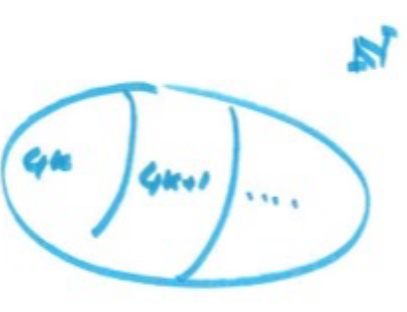
\includegraphics[scale=0.4]{images/rel_equi_quot.png}
    \caption{Insieme quoziente di $\equiv_4$}
\end{figure}

$\{[i]_4 : 0\leq i\leq 3\}$ è una partizione di $\mathbb{N}$ indotta dalla relazione
$\equiv_4$, tale per cui mi dia il rispettivo insieme quoziente (a volte impropriamente
chiamato $\mathbb{Z}_4$):
$$N / \equiv_4 \text{ }=\{[i]_4 : 0\leq i\leq 3\}=\mathbb{Z}_4$$
Adesso abbiamo in mano gli strumenti per definire in maniera molto più fine il concetto
di cardinalità.
\subsubsection{Cardinalità degli insiemi - II°}
Sia $\mathcal{U}$ (insieme universo) la classe di tutti gli insiemi,
definiamo la relazione $\sim\subseteq\mathcal{U}^2$ detta relazione
di \textit{equi numerosità} (hanno la stessa dimensione numerica), tra le coppie degli insiemi, se e solo se esiste
una \textbf{biezione} tra $A$ e $B$ (ovvero, se riesco ad esibire una funzione
iniettiva e suriettiva che va da $A$ in $B$).
Questa relazione tra insiemi è una relazione di equivalenza, poiché:
\begin{itemize}
    \item $\sim$ è riflessiva, se utilizzo la funzione identità $i_A$.
    \item $\sim$ è simmetrica, se esiste una biezione $A\rightarrow B$ allora
          esiste una biezione anche $B\rightarrow A$. Ovvero $A\sim B$ e $B\sim A$.
    \item $\sim$ è transitiva, se compongo funzioni biettive ottengo ancora una
          funzione biettiva.
\end{itemize}

Sue insiemi che stanno in questa relazione vengono detti \textbf{equi numerosi}. Ora
considerando l'insieme quoziente del nostro universo $\mathcal{U}$ rispetto alla
relazione di equi numerosità $\sim$ (quindi stesso numero di elementi in entrambi
i due insiemi), esso mi rappresenta il concetto di \textbf{cardinalità}
di un insieme rispetto ad un altro.
\begin{figure}[H]
    \centering
    \includegraphics[scale=0.4]{images/insieme_quoziente_cardinalità.png}
    \caption{Insieme quoziente $\mathcal{U} / \sim$}
\end{figure}
Quindi spezzettando l'insieme $\mathcal{U}$ in classi di equivalenza
in questa classe di equivalenza ci sono tutti gli insiemi
che sono equi numerosi (seppur diversi).
Questo concetto mi permetterà anche di parlare in maniera molto precisa anche di
insiemi di cardinalità infinita.
\newline
\newline
Per esempio, consideriamo $n\in\mathbb{N}^+$, si consideri l'insieme $J_n=\{1,2,...,n\}$. Per questo
insieme è ovvio quale sia il concetto di cardinalità perchè è finito.
Allora diciamo che un insieme $A$ ha cardinalità \textbf{finita} se è equi
numeroso con $J_n$ (ovvero $A\sim J_n$) per un dato $n$ ed in quel caso scriviamo che $|A|=n$.

Quindi nella classe di equivalenza $J_1$ troviamo tutti gli insiemi con un
elemento, nella classe di equivalenza di $J_2$ troveremo tutti gli insiemi con due elementi, ecc.
\begin{figure}[H]
    \centering
    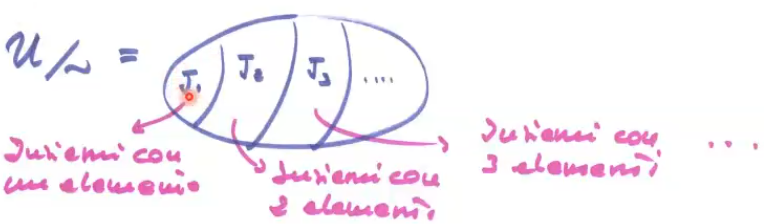
\includegraphics[scale=0.5]{images/U_insiemi_esemp_card2.png}
    \caption{Esempio $\mathcal{U}/\sim$ rispetto all'insieme $J_n$}
\end{figure}
Un insieme che non ha cardinalità si dice banalmente che ha cardinalità \textbf{infinità}. Fin qui abbiamo
parlato ancora di cardinalità finita, ma adesso faremo un esempio con cardinalità infinita.

\subsubsection{Insiemi numerabili}
$A$ si dice \textbf{numerabile} se è nella stessa classe di equivalenza dell'insieme dei numeri naturali
$\mathbb{N}$, ovvero se esiste una relazione di \textbf{equinumerosità} tra l'insieme $A$ e l'insieme $\mathbb{N}$.
$$A\sim\mathbb{N}$$
Siccome stanno in relazione di equi numerosità
vuol dire che è presente una biezione fra i due elementi, quindi due elementi non possono collidere.
\begin{figure}[H]
    \centering
    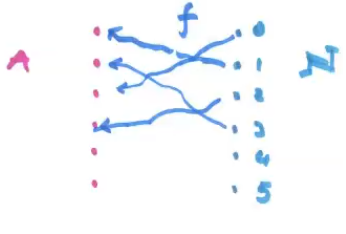
\includegraphics[scale=0.6]{images/A_numerabile_N.png}
    \caption{$A$ è un insieme numerabile}
\end{figure}
La presenza di questa biezione significa che come $A$ può essere \textbf{listato} con
$f(0),f(1),f(2),...$ su $\mathbb{N}$ senza perdere un elemento, anche l'insieme $\mathbb{N}$ può essere
listato a sua volta su $A$.
Alcuni esempi di insiemi numerabili:
\begin{itemize}
    \item I numeri pari $f(n)=2n$ , essi sembrerebbero la metà dei numeri naturali ma sono tanti quanto i numeri
          naturali perchè esiste questa biezione (vale anche per i dispari $f(n)=2n+1$).
    \item L'insieme $\mathbb{Z}$, possono essere presenti diverse funzioni, per esempio
          posso mappare i negativi sui numeri pari ed i positivi sui numeri dispari.
    \item L'insieme $\mathbb{Q}$, vedremo più avanti.
    \item L'insieme delle stringhe binarie che incominciano con $1$, ovvero $1\{0,1\}^*$,
          dove una funzione $f(n)=bin(n)$ è in grado di associare un numero naturale (utilizzando
          le potenze in posizione) ad una stringa binaria.
\end{itemize}

\subsection{Insiemi non numerabili}
Esistono degli insiemi che non sono listabili, dette in altre parole sono più fitti di $\mathbb{N}$,
è un altro tipo di categoria di infinito.
$$A\nsim\mathbb{N}$$
$\mathbb{R}$ è un insieme non numerabile.
\paragraph{Dimostrazione}\mbox{}\\
L'idea consiste nel dimostrare per assurdo che non esiste una biezione
perchè sono presenti dei "buchi" tra le associazioni. Ordine della dimostrazione:
\begin{itemize}
    \item Dimostro che $\mathbb{R}\sim[0,1]$ (si dice che è \textit{isomorfo/equi numeroso} all'intervallo $[0,1]$),
          ovvero che è fitto quanto l'intervallo citato.
    \item Dimostro che $\mathbb{N}\nsim[0,1]$
    \item $\mathbb{R}\sim[0,1]\nsim\mathbb{N}\implies\mathbb{R}\nsim\mathbb{N}$
\end{itemize}

\paragraph{Dimostrazione $R\sim[0,1]$}\mbox{}\\
Significa riuscire a rappresentare una funzione
che mappa gli elementi tra i due insiemi in maniera che sia suriettiva ed iniettiva.
Prima di tutto abbiamo una retta cartesiana con un origine fissata e che copre tutti i numeri reali.
Pongo l'intervallo $[0,1]$ in modo che si trovi in corrispondenza del punto mediano della retta $0$,
successivamente prendo un compasso punto il centro nel mediano dell'intervallo e traccio la
semi circonferenza rispetto alla metà dell'intervallo.
\begin{figure}[H]
    \centering
    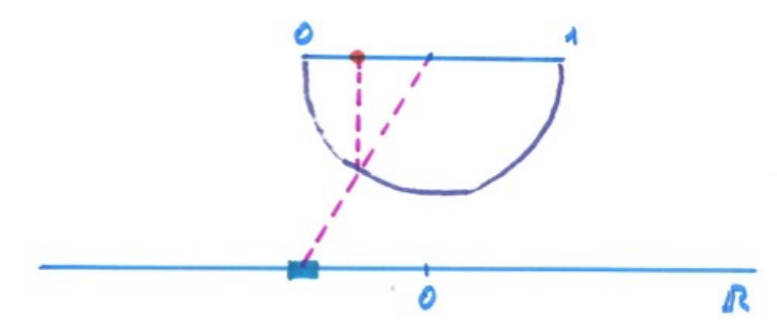
\includegraphics[scale=0.5]{images/dim_1.png}
    \caption{Dimostrazione  $R\sim[0,1]$}
\end{figure}
Gli elementi dell'insieme $\mathbb{R}$ vengono mappati tracciando una retta in direzione del punto
mediano di $[0,1]$, nel punto di intersezione si traccia la retta perpendicolare che interseca
l'intervallo ed in quel punto si trova il valore corrispondente. Si può fare lo stesso
in maniera opposta partendo da $[0,1]$, trovando l'intersezione si parte dal punto mediano
di quest'ultima e si attraversa l'intersezione toccando $\mathbb{R}$.
Questo dimostra che tutti i valori di $\mathbb{R}$ sono associabili
su $[0,1]$, quindi $\mathbb{R}\sim[0,1]$.

\paragraph{Dimostrazione $\mathbb{N}\nsim[0,1]$ (per diagonalizzazione)}\mbox{}\\Supponiamo per assurdo che $\mathbb{N}\sim[0,1]\implies[0,1]$,
ovvero che sia listabile (\textit{elencabile}) in maniera esaustiva così come lo è $\mathbb{N}$.
Siccome sto ipotizzando che sia elencabile, allora creo una lista di tutti gli elementi in $[0,1]$, i numeri
all'interno di questo numero seguono il formato "$0.$", quindi:
\[
    \begin{array}{ccccc}
        \underline{0.a_{11}} & a_{12}             & a_{13}             & a_{14}             & ... \\
        0.a_{21}             & \underline{a_{22}} & a_{23}             & a_{24}             & ... \\
        0.a_{31}             & a_{32}             & \underline{a_{33}} & a_{34}             & ... \\
        0.a_{41}             & a_{42}             & a_{43}             & \underline{a_{44}} & ... \\
        ...                  & ...                  & ...                  & ...                  & ... \\
    \end{array}
\]
Se riesco a costruire un numero che non fa parte di questa lista infinita (elusivo alla biezione),
allora vuol dire che la lista non è elencabile, e quindi $[0,1]$ non è numerabile.
Per costruire questo numero elusivo che non si trova in nessuno di questi elementi della lista,
vado a guardare le cifre sulla \textit{diagonale}.\\Costruiamo il numero elusivo alla lista
$$0.c_1c_2c_3c_4$$
Tale che rispetti la seguente regola rispetto alla diagonale del elenco dei numeri $\in [0,1]$
\[
    c_i=
    \begin{cases}
        a_{ii} + 1\text{ se }a_{ii} < 9 \\
        a_{ii} - 1\text{ se }a_{ii} = 9 \\
    \end{cases}
\]
Ora usando questa regola non riuscirò mai a posizionare il mio nuovo numero
tra quelli elencati, questo perchè ovviamente cambio le cifre (il perché questo accade
probabilmente è collegato al fatto che $\mathbb{R}$ è più fitto di $\mathbb{N}$, proprio
quello che vogliamo dimostrare).
Il numero $0.c_1c_2...\in[0,1]$, ma non appartiene nelle liste poiché:
\begin{itemize}
    \item Differisce dal primo perché $c_1\neq a_{11}$
    \item Differisce dal secondo perché $c_2\neq a_{22}$
    \item Differisce da qualunque numero presente sulla diagonale
\end{itemize}
Quindi la lista non è esaustiva $\implies \mathbb{N}\nsim[0,1]$, significa che non cattura tutto l'intervallo $[0,1]$,
quindi non può esistere una biezione tra questo ed $\mathbb{N}$, ovvero $[0,1]$ \textbf{non è numerabile}.

\paragraph{Conclusione}\mbox{}\\
$$\mathbb{R}\sim[0,1]\nsim\implies\mathbb{R}\nsim\mathbb{N}$$
\begin{itemize}
    \item $\mathbb{R}$ non è numerabile.
    \item Esso è più \textit{"fitto"} di $\mathbb{N}$.
    \item Qualsiasi tentativo di listare anche solo un segmento non è esaustivo.
    \item $\mathbb{R}$ è un insieme \textbf{continuo}, e tutti gli insiemi equi numerosi
          $\mathbb{R}$ si dicono continui.
    \item Altri esempi di insiemi non numerabili:
\end{itemize}

\subsubsection{Insieme delle parti di $\mathbb{N}$}
Un altro insieme non numerabile è quello costituito dalla famiglia di sottoinsiemi possibili di $\mathbb{N}$,
quindi mettendo assieme uno dopo l'altro tutti i sottoinsiemi di differenti cardinalità (talvolta chiamato
\textbf{insieme potenza} o \textbf{booleano di} $\mathbb{N}$). Per esempio su un insieme $S=\{a,b,c\}$,
l'insieme delle parti è $\mathcal{P}(S)=\{\emptyset,\{a\},\{b\},\{c\},\{a,b\},\{a,c\},\{b,c\},S\}$.
$$\mathcal{P}(\mathbb{N})=2^{\mathbb{N}} = \{\text{sottoinsiemi di }\mathbb{N}\}\nsim\mathbb{N}$$
Anche questa dimostrazione avviene per diagonalizzazione, per assurdo suppongo che esista una
biezione che mi permetta di elencare tutti i sottoinsiemi di $\mathbb{N}$.
Posso rappresentare i sotto insiemi di $\mathbb{N}$ utilizzando un \textbf{vettore caratteristico}
$A\subseteq\mathbb{N}$, questo è un vettore dove metto il bit di appartenenza rispetto alla corrispondenza
dell'elemento.
\[
    \mathbb{N}\rightarrow
    \begin{array}{cccccccc}
        0 & 1 & 2 & 3 & 4 & 5 & 6 & ... \\
    \end{array}
\]
\[
    A\rightarrow
    \begin{array}{cccccccc}
        0 & 1 & 1 & 0 & 1 & 1 & 0 & ... \\
    \end{array}
\]
Allora se io suppongo per assurdo che $\mathcal{P}(\mathbb{N})\sim\mathbb{N}$, ovvero che è numerabile
rispetto all'insieme dei numeri naturali, allora posso elencare in maniera esaustiva i sotto insiemi
di $\mathbb{N}$, questo elencandone i vettori caratteristici.
\[
    \begin{array}{ccccc}
        \underline{b_{11}} & b_{12}             & b_{13}             & b_{14}             & ... \\
        b_{21}             & \underline{b_{22}} & b_{23}             & b_{24}             & ... \\
        b_{31}             & b_{32}             & \underline{b_{33}} & b_{34}             & ... \\
        b_{41}             & b_{42}             & b_{43}             & \underline{b_{44}} & ... \\
        ...                  & ...                  & ...                  & ...                  & ... \\
    \end{array}
\]
Se riesco a costruire un sottoinsieme di $\mathbb{N}$ (vettore caratteristico) che non fa parte da di questa lista,
allora l'insieme delle parti non è un insieme numerabile poiché non è equi-numeroso con $\mathbb{N}$. Questo
è possibile procedendo per \textit{diagonalizzazione}, per esempio se considerassi il seguente vettore negato:
\[
    \begin{array}{ccccc}
        \overline{b_{11}} & \overline{b_{22}} & \overline{b_{33}} & \overline{b_{44}} & ... \\
    \end{array}
\]
riesco a constatare che esso non appartiene alla lista nonostante sia un sottoinsieme di $\mathbb{N}$
in quanto composto solo da valori booleani.
$$\mathcal{P}(\mathbb{N})\nsim\mathbb{N}$$
\subsubsection{Insieme $\mathbb{N}^{\mathbb{N}}$}
Consideriamo l'insieme di tutte le funzioni possibili che vanno da $\mathbb{N}$ in $\mathbb{N}$.
$$\mathbb{N}^{\mathbb{N}}=\{f:\mathbb{N}\rightarrow\mathbb{N}\}$$
Ipotizzando che $\mathbb{N}^{\mathbb{N}}$ sia numerabile ($\mathbb{N}^{\mathbb{N}}\sim\mathbb{N}$),
consideriamo la seguente tabella dove nella prima
colonna si trova l'elenco esaustivo di tutte le funzioni $\in\mathbb{N}$, e nelle colonne successive tutto
il dominio completo di $\mathbb{N}$. Significa che per ogni riga sara presente l'insieme dei valori che
fornisce il grafico di una funzione $f_i$.
\begin{center}
    \begin{tabular}{c|ccccc}
        \toprule
        Elenco delle funzioni di $\mathbb{N}$ & \textbf{0}           & \textbf{1}           & \textbf{2}           & \textbf{3}            & \textbf{...$\in\mathbb{N}$} \\
        \midrule
        $f_0$                                 & $\underline{f_0(0)}$ & $f_0(1)$             & $f_0(2)$             & $f_0(3)$              & $...$                       \\
        $f_1$                                 & $f_1(0)$             & $\underline{f_1(1)}$ & $f_1(2)$             & $f_1(3)$              & $...$                       \\
        $f_2$                                 & $f_2(0)$             & $f_2(1)$             & $\underline{f_2(2)}$ & $f_2(3)$              & $...$                       \\
        $f_3$                                 & $f_3(0)$             & $f_3(1)$             & $f_3(2)$             & $\underline{f_ 3(3)}$ & $...$                       \\
        $...$                                 & $...$                & $...$                & $...$                & $...$                 & $\underline{...}$           \\
        \bottomrule
    \end{tabular}
\end{center}
Allora anche in questo caso per diagonalizzazione voglio costruire una funzione $\in\mathbb{N}^{\mathbb{N}}$ ma
elusiva all'elenco delle funzioni della tabella:
$$\varphi:\mathbb{N}\rightarrow\mathbb{N}\text{ come }\varphi(n)=f_n(n)+1$$
Siamo d'accordo che $\varphi$ sia ben definita, visto che per ogni immagine corrisponderà un immagine numero naturale,
ma notiamo che una qualsiasi $\varphi(n)$ presa sulla lista avrà per forza una immagine della diagonale discordante
rispetto a quelle elencate nella tabella.\\ Quindi abbiamo una funzione elusiva all'elenco, e la nostre ipotesi si rivela assurda:
$$\varphi(0)=f_0(0)+1\neq f_0(0)$$
$$\mathbb{N}^{\mathbb{N}}\nsim\mathbb{N}$$
N.B.: Gli insiemi $\mathcal{P}(\mathbb{N})$ e $\mathbb{N}^{\mathbb{N}}$ sono detti \textbf{insiemi continui},
e sono equi numerosi a $\mathbb{R}$.

\section{Teoria della calcolabilità}
\subsection{Cosa è calcolabile?}
Sappiamo che la potenza computazionale di un sistema di calcolo $\mathcal{C}$ corrisponde a:
$$F(\mathcal{C})=\{\mathcal{C}(P,\_):P\in PROG\}\subseteq DATI_{\bot}^{DATI}$$
Il nostro problema consiste nel comprendere se questa inclusione sia propria o impropria,
per dimostrare ciò posso utilizzare il concetto di cardinalità precedentemente appreso.\\
Se riesco a dimostrare che il primo insieme ha una cardinalità numerabile ed il secondo ha
una cardinalità continua allora il secondo insieme sarà molto più grande del primo.\\Prendiamo alcune
\textbf{assunzioni} che verranno dimostrate successivamente nel corso:
\begin{itemize}
    \item $PROG\sim\mathbb{N}$, i programmi sono tanti quanti i numeri naturali, questo
          perché un programma viene digitalizzato in una fila di bit (finiti). Questo vuol dire che per ogni
          programma corrisponderà un numero che fa parte dei numeri naturali.

    \item $DATI\sim\mathbb{N}$, i dati sono tanti quanto i numeri, questo per lo stesso motivo
          di digitalizzazione (o traduzione) in binario delle informazioni.
\end{itemize}
Possiamo dire che la potenza computazionale sia equinumerosa rispetto al numero di programmi,
al variare del programma cambio la funzione di potenza computazionale. A questo punto agganciamo
la prima assunzione.
$$F(\mathcal{C})\sim PROG\sim\mathbb{N}$$
Sapendo che l'insieme dei dati in dati definito come $DATI_{\bot}^{DATI}$, grazie alla
seconda assunzione che abbiamo fatto allora possiamo asserire:
$$DATI_{\bot}^{DATI}\sim\mathbb{N}_{\bot}^{\mathbb{N}}$$

Abbiamo visto precedentemente che $\mathbb{N}^{\mathbb{N}}\nsim\mathbb{N}$, allora unendo le precedenti
dimostrazioni possiamo confermare:
$$F(\mathcal{C})\sim PROG\sim\mathbb{N}\nsim\mathbb{N}^{\mathbb{N}}\sim DATI_{\bot}^{DATI}$$
$$F(\mathcal{C})\nsim DATI_{\bot}^{DATI}$$
Ovvero, che l'insieme dei programmi (corrispondente all'insieme delle funzioni di potenza di calcolo)
non è equinumeroso (o \textit{isomorfo}) all'insieme delle funzioni che vanno da dati in dati. In parole
povere ho un numero di programmi nettamente inferiore (fitto quanto i numeri naturali) rispetto al numero
di funzioni (o problemi) calcolabili (fitto quanto i reali $\mathbb{N}_{\bot}^{\mathbb{N}}$).

\subsubsection{Dimostrazione $DATI\sim\mathbb{N}$}
Vogliamo stabilire una corrispondenza \textbf{biunivoca} tra dati e numeri naturali, ovvero
che devo riuscire a "nascondere" un dato all'interno di un numero naturale, tale che
se lo dovessi riportare all'insieme dei dati otterrei esattamente quel dato (e non un altro).

Questa biezione la voglia rendere effettiva e programmabile, ovvero costruirci delle primitive che
operino direttamente sulla codifica numerica dei dati così che possiamo smaterializzare completamente
il mondo dei dati in quello dei numeri.

Questa volta vogliamo dimostrare che l'\textbf{insieme delle coppie} $\mathbb{N}\times\mathbb{N}$
è numerabile. Questo avverrà per passi, prima dimostreremo che l'insieme delle coppie è isomorfo a
$\mathbb{N}^+$ (quindi escluso lo $0$) e poi di conseguenza che lo è per tutto $\mathbb{N}$.
Questo per effetto collaterali che anche l'insieme dei razionali $\mathbb{Q}$ è numerabile,
questo perché sono una frazione, quindi una coppia di interi.
\paragraph{Dimostrazione $\mathbb{N}\times\mathbb{N}\sim\mathbb{N}^+$}\mbox{}\\
$$\langle ,\rangle :\mathbb{N}\times\mathbb{N}\rightarrow\mathbb{N}^+$$
$$\langle x,y\rangle =n$$
La \textbf{funzione coppia di Cantor} è definita per mezzo delle parentesi
angolari, prende due argomenti $x,y$ e restituisce un numero $n$, questo
in maniera iniettiva e suriettiva (biettività).

Ovvero che coppie diverse vengono mappate in numeri diversi, e se
ho un numero devo essere in grado di tornare alla stessa coppia $x,y$. Quindi esibiremo sia
l'andata della funzione coppia di Cantor che il ritorno, esibiremo anche i due proiettori
\textit{sin} e \textit{des} tali che mi restituiscano i due argomenti in questione.
$$sin:\mathbb{N}^+\rightarrow\mathbb{N}\text{ e }des:\mathbb{N}^+\rightarrow\mathbb{N}$$
$$sin(n)=x\text{ e }des(n)=y$$
Vogliamo dare una rappresentazione grafica di questa funzione, Cantor ha pensato di realizzare
una tabella che ha come righe e colonne l'insieme $\mathbb{N}$. In questa tabella
il valore della coppia si trova esattamente posizionato all'incrocio tra l'$x$-esima riga
e della $y$-esima colonna.
\[
    \begin{tabular}{c|ccccc}
        x/y & 0  & 1   & 2   & 3   & 4   \\
        \midrule
        0   & 1  & 3   & 6   & 10  & 15  \\
        1   & 2  & 5   & 9   & 14  & ... \\
        2   & 4  & 8   & 13  & ... & ... \\
        3   & 7  & 12  & ... & ... & ... \\
        4   & 11 & ... & ... & ... & ... \\
    \end{tabular}
\]
La disposizione ingegnosa della tabella evita di andare in un elenco infinito,
nel senso che se dovessi elencare tutti i numeri naturali andando verso il basso (o
destra) non riuscirei a finire mai, ed inoltre non sarebbe un buon approccio visuale per trovare
la corrispondenza con l'altro insieme. I numeri sono disposti in maniera che il successivo
si trovi sulla diagonale (andando verso l'alto).
$$\langle 2,1\rangle =8$$
Con questa rappresentazione, coppie diverse non riusciranno mai a confluire nella stessa
casella (coordinate di punti che individuano un punto univoco), e viceversa (iniettiva),
questo mi conferma che la funzione è biettiva.\\Adesso mettiamo da parte la forma tabellare e
consideriamo la \textbf{forma analitica} di $\langle ,\rangle $.
\begin{figure}[H]
    \centering
    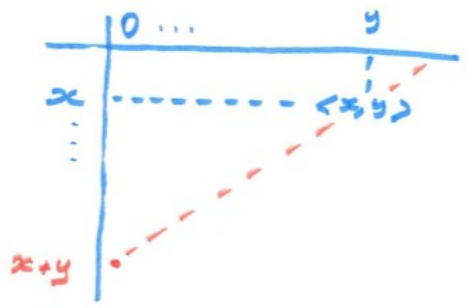
\includegraphics[scale=0.5]{images/coord_dim.png}
    \caption{Diagonale che passa per $\langle x,y\rangle $}
\end{figure}
Notiamo che per il valore che voglio valutare attraverso la funzione di Cantor passa una diagonale,
questa diagonale parte dalla colonna $0$ e dalla riga $x+y$ (il punto $\langle x+y,0\rangle $). La funzione
coppia nell'origine della diagonale assumerà un certo valore, e visto che i numeri sulla
diagonale incrementano in maniera crescente di una sola unità, allora potrò raggiungere $\langle x,y\rangle $
sommando $y$.\\A questo punto il mio problema si riduce a trovare delle coppie particolari ovvero,
la cui seconda coordinata è $0$, le chiamiamo $\langle z,0\rangle$. Notiamo nella prima colonna
c'è una correlazione con gli elementi di $x$, e vediamo che l'elemento $i$-esimo della prima
colonna corrisponde alla somma tra il corrispettivo elemento $x$ e l'elemento $i-1$ della colonna,
allora riusciamo ad esprimere una \textbf{legge matematica} per descrivere questa \textit{codifica}.

\begin{enumerate}
    \item $\langle x,y\rangle =\langle x+y,0\rangle +y$
    \item $\langle z,0\rangle ? \implies \langle z,0\rangle = \sum_{i=1}^z i+1=\frac{z(z+1)}{2}+1$
\end{enumerate}
\noindent Allora $(1)+(2)$:
$$\langle x,y\rangle = \langle x+y,0\rangle+y=\frac{(x+y)(x+y+1)}{2}+y+1$$

\paragraph{Come tornare da $\mathbb{N}^2$ a $\mathbb{N}^+$}
Ovvero, come trovare le funzioni $sin$ e $des$.
$$\langle x,y \rangle = n \longrightarrow sin(n)=x \text{ e } des(n)=y$$
\begin{figure}
    \centering
    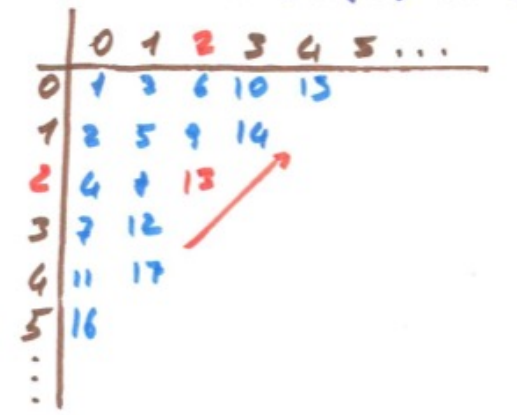
\includegraphics[scale=0.5]{images/coord_dim_2.png}
    \caption{$n=13$}
\end{figure}

Partiamo da un elemento $n$ presente nell'intersezione dei due insiemi definiti da
$x$ e $y$ e vogliamo individuare le due relative componenti. Procedo trovando
le coordinate dell'origine della diagonale che passa per $n$, ovvero $\langle\gamma ,0\rangle$.
Considerando la dimostrazione precedente possiamo dire che $y = n-\langle\gamma ,0\rangle$, ovvero
procedo a ritroso sulla diagonale partendo da $n$ ed andando verso $\langle\gamma ,0\rangle$.\\Allora,
sapendo che $\gamma=x+y$ posso trovare facilmente le parti destre e sinistre.\\ Il problema principale
ora è trovare $\gamma$, questo non è altro che l'intero più grande tale per cui l'origine
della diagonale sia minore di $n$.
$$\gamma = \max\{z\in\mathbb{N}:\langle z,0\rangle\leq n\}$$
Quindi dobbiamo risolvere la disuguaglianza la quale ci darà un range su $n$, all'interno di questo
range $\langle z,0\rangle\leq n$ andiamo a prendere l'intero più grande che soddisfa questa disuguaglianza.
$$\langle z,0\rangle\leq n\longrightarrow\frac{z(z+1)}{2}+1\leq n\longrightarrow z^2+z+2-2n\leq 0$$
$$z_{1,2}=\frac{-1 \pm\sqrt{8n-7}}{2}$$
Quindi devo scoprire quale è l'intero più grande dati:
$$\frac{-1 -\sqrt{8n-7}}{2}\leq z\leq \frac{-1 +\sqrt{8n-7}}{2} $$
l'elemento a destra è il più grande valore, ma non so se è intero, quindi dovrò correggere ciò:
$$\gamma=\left\lfloor\frac{-1+\sqrt{8n-7}}{z} \right\rfloor$$
Questa è un formula che utilizza la variabile in input $n$, quindi riusciamo a ricavare il parametro
sinistro e destro della funzione di Cantor e ritornare allo stato iniziale:
$$des(n)=y=n-\langle\gamma ,0\rangle \text{ e }sin(n)=x=\gamma -y$$

\paragraph{Esempio andata e ritorno tra $\mathbb{N}^2$ e $\mathbb{N}^+$}
$$\text{Andata : }\mathbb{N}^2 \longrightarrow\mathbb{N}^+$$

$$\langle 10,20\rangle = \frac{30\cdot31}{2}+20+1=15\cdot31+21=485+21=486$$

$$\text{Ritorno : }\mathbb{N}^+\longrightarrow\mathbb{N}^2$$F
$$\gamma = \left\lfloor \frac{-1 + \sqrt{8 \cdot 486-7}}{2} \right\rfloor = \lfloor 30.6448\rfloor = 30$$
$$y=486- \langle 30,0\rangle = 486- \left(\frac{30\cdot31}{2}+1\right)=486-466=20=des(486)$$
$$x=30-20=10=sin(486)$$
Adesso noi abbiamo dimostrato che $\mathbb{N}^2\sim\mathbb{N}^+$.

\paragraph{Dimostrazione $\mathbb{N}\times\mathbb{N}\sim\mathbb{N}$}
Definisco una nuova funzione:
$$[,]:\mathbb{N}\times\mathbb{N}\text{ tale che }[x,y]=\langle x,y\rangle-1$$
Adesso ho una funzione esplicita per mappare $\mathbb{N}^2$ su $\mathbb{N}$.\\Nota: A questo
punto otteniamo che l'insieme dei razionali $\mathbb{Q}$ sono coppie di interi $(num,den)$. Dunque
$[,]$ mostra che $\mathbb{Q}$ è numerabile.

\paragraph{Dimostrazione rigorosa che $DATI\approxeq\mathbb{N}$}
Mostriamo le nozioni appena apprese sulle principali strutture dati.
\paragraph{Liste d'interi}\mbox{}\\
$$\textit{codifichiamo } x_1,x_2,...,x_n\rightarrow\langle x_1,x_2,...,x_n\rangle$$
Quindi il numero che rappresenta la codifica è indicato con il numero all'interno delle parentesi angolari.
L'idea consiste nell'incapsulare il risultato di una coppia di elementi come elemento destro
della coppia più esterna. Non sapendo quanto sia lunga la lista dovrò porre un elemento che mi
segnali il termine, e questo lo posso fare con $\langle x_n,0 \rangle$.

$$\langle x_1,x_2,...,x_n\rangle = \langle x_1,\langle x_2,\langle ...\langle x_n,0\rangle ...\rangle\rangle\rangle$$

\noindent Per esempio:
$$\textit{codifica }1,2,5\rightarrow\langle 1,2,5\rangle=\langle 1,\langle 2,\langle 5,0\rangle\rangle\rangle=$$
$$\langle 1,\langle2,16\rangle\rangle=\langle 1,188\rangle=$$
$$=18144$$
Per l'operazione di decodifica quello che facciamo è di considerare la codifica della mia lista $M$ (non il
risultato ma la lista di coppie incapsulate) come un albero binario.
\begin{figure}[H]
    \centering
    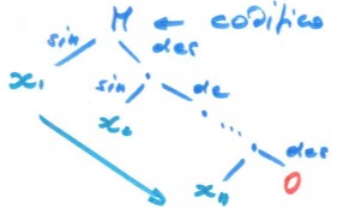
\includegraphics[scale=0.5]{images/bin.png}
\end{figure}

Allora dato questo albero il figlio
sinistro è l'elemento sinistro (la testa della lista) ed il figlio destro è la parte restante della lista,
allora continuando a considerare il figlio sinistro come una struttura dati lineare ottengo
la lista codificata, questo attraversamento dell'albero in pre-ordine terminerà quando incontrerà un
figlio destro $0$ (l'ultimo elemento, c'è solo un elemento  con $0$).\\Vogliamo effettuare
delle implementazione in pseudo-codice (simile C), assumiamo $0$ come la lista nulla, e $\langle,\rangle,sin,des$
come la funzione di Cantor $\langle , \rangle$.
\paragraph{Implementazione codifica}\mbox{}
\begin{lstlisting}[mathescape=true]
int encode($x_1,...,x_n$){
    int $k$ = 0;
    for(int $i$ = $n$; $i$ >= 1; $i$--)
        $k$ = $\langle x_i,k\rangle$;
    return $k$;
}
\end{lstlisting}
\paragraph{Implementazione decodifica}\mbox{}
\begin{lstlisting}[mathescape=true]
void decode(int $n$){
    if($n$!=0){
        print($sin(n)$);
        decode($des(n)$);
    }
}
\end{lstlisting}

Altre operazioni utili possono essere sono quelle per calcolare la \textbf{lunghezza}:
\begin{lstlisting}[mathescape]
int length(int n){
    return $n$==$0$ ? $0$ : $1$ + length($des(n)$);
}
\end{lstlisting}
Oppure per calcolare la \textbf{proiezione}:
\[
    proj(t,b)=
    \begin{cases}
        -1  & \text{se } t>length(n)\text{ o }t==0                                           \\
        x_t & \text{se }1\leq t\leq length(n)\text{ e }n=\langle x_1,...,x_t,..., x_m\rangle
    \end{cases}
\]
\begin{lstlisting}[mathescape]
int proj(int $t$, int $n$){
    if ($t$ == $0$ || $t$ > length($n$))
        return $-1$;
    else {
        if ($t$ == $1$)
            return $sin(n)$;
        else
            return proj($t-1$,$des(n)$);
    }
}
\end{lstlisting}
\paragraph{Esercizi - $incr,decr$ (da implementare)}\mbox{}
\[incr(t,n)=
    \begin{cases}
        -1                                    & \text{se }t>length(n)\text{ o }t==0                                            \\
        \langle x_1, ...,x_t+1,...,x_n\rangle & \text{se } 1\leq t\leq length(n)\text{ e }n=\langle x_1,...,x_t,...,x_m\rangle
    \end{cases}
\]
$decr(t,n)=\text{ come sopra ma con }\langle x_1,...,x_t-1,...,x_m\rangle$

\paragraph{Corrispondente numerico : $DATI\sim\mathbb{N}$}\mbox{}\\
Adesso sappiamo codificare liste di interi, questo ci da un idea del fatto che i dati siano
isomorfi ad $\mathbb{N}$. Questo ci da un modo per nascondere testi, suoni, immagini dietro ad
un numero. Per esempio, per compattare un testo in un numero posso imporre una codifica (tipo
ASCII), in questa maniera posso associare un numero per ogni carattere numerico, un insieme
di caratteri numerici è codificabile utilizzando $\langle , \rangle$ il quale mi darà un
singolo numero.
\begin{figure}[H]
    \centering
    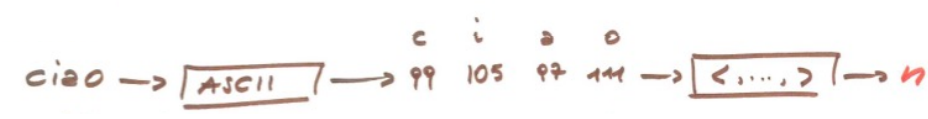
\includegraphics[scale=0.4]{images/test_codifica.png}
    \caption{Codifica di un testo}
\end{figure}
\textit{Posso usare questo modo per comprimere i testi?} In realtà questa tecnica non
è un buon compressore, questo perché la crescita del numero è quadratica rispetto
al numero di caratteri codificati (otteniamo un $n$ troppo grande e si verifica un espansione,
altroché). \textit{Perché non è un buon modo per crittografare i dati?} Il primo problema
è che il testo crittografato sarebbe molto lungo (aumenta il rischio nella perdita
di dati durante la trasmissione), secondo problema la coppia di Cantor è una funzione biettiva,
esiste un modo abbastanza diretto per tornare indietro.
\begin{figure}[H]
    \centering
    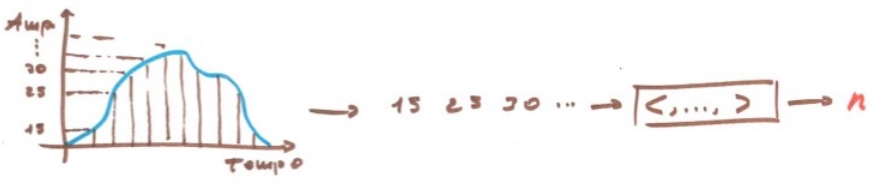
\includegraphics[scale=0.4]{images/suono_codifica.png}
    \caption{Discretizzazione del suono in segnale digitale e poi codifica in numero naturale}
\end{figure}
Per i suoni il discorso è molto simile, grazie alla \textbf{campionatura} (o
\textbf{discretizzazione}) dei segnali analogici in un segnale digitale, ovvero una grandezza
discreta sotto forma di numeri naturali.\\Per le immagini potrei usare la tecnica bitmap,
quindi per ogni bit registro un colore che verrà codificato con un numero (e da qui come per
gli altri casi sappiamo come muoverci).

\paragraph{Codifica di altre stutture dati}\mbox{}\\
Codifica di un \textbf{array} a dimensione finita, proprio per questo non necessità di
un elemento che mi ponga fine alla sequenza (so già dove fermarmi).
$$x_1,...,x_n\rightarrow[x_1,...,x_n]$$
$$[x_1,...,x_n]=[x_1,...,[x_{n-1},x_n]]...]$$
Codifica di una \textbf{matrice}, esse sono array bidimensionali dove hanno anch'esse
dimensione fissa e nota. Quindi mi basta codificare per riga le matrici e poi codificare
le codifiche.
\[
    \begin{bmatrix}
        x_{11} & x_{12} \\
        x_{21} & x_{22} \\
    \end{bmatrix}
    =\left[[x_{11},x_{12}],[x_{21},x_{22}]\right]
\]
Sia per la codifica di array che per quello delle matrici sono facilmente implementabili
le primitive numeriche ad esempio $elem(i,j,n)$ che restituisce l'elemento $(i,j)$-esimo
di una matrice codificata dal numero $n$.\\Codifica dei \textbf{grafi}, sappiamo
che un grafo è rappresentabile con lista di adiacenza, matrice di adiacenza,...
quindi possiamo codificare la lista o la matrice.
\paragraph{Conclusione}\mbox{}\\
Abbiamo mostrato effettivamente che grazie alla
corrispondenza effettiva di $DATI\sim\mathbb{N}$ che i dati possono essere "scartati" e tenuti solamente i
numeri, questo perché ogni dato può essere rappresentato con un numero naturale, questo
grazie a delle leggi matematiche effettive ed implementabili, che mi
permettono di codificare e decodificare il dato.\\Quindi la nostra funzione $f:DATI\rightarrow DATI_{\bot}$
che rappresenta un qualsiasi problema, può essere sostituita da una funzione $f:\mathbb{N}\rightarrow\mathbb{N}_\bot$,
ed è questo quello che i nostri calcolatori calcoleranno, quindi possiamo dire che il nostro universo
dei problemi $DATI^{DATI}_\bot$ non è altro che $\mathbb{N}^{\mathbb{N}}_\bot$

\subsubsection{Prefazione alla dimostrazione $PROG\sim\mathbb{N}$}
Per spiegare ciò utilizzeremo un linguaggio apposito detto
\textit{"linguaggio RAM"} e su un sistema formale apposito detto \textit{"sistema RAM"}.
Grazie alla semplicità di questo potrò mostrare molto semplicemente:
\begin{itemize}
    \item Che i programmi sono numerabili $PROG\sim\mathbb{N}$
    \item In maniera rigorosa la semantica dei programmi, $\mathcal{C}(P,\_)\rightarrow RAM(P,\_)$
    \item Ed altrettanto formalmente potrò definire la potenza computazionale $F(RAM)$, questo fornirà
          un idea di \textit{che cosa è calcolabile}.
\end{itemize}
Il linguaggio RAM è un \textit{assembly} molto semplificato, per questo motivo l'idea di
calcolabilità è altamente criticabile, poiché il modello potrebbe fare scappare qualcosa
per via della banalità.

Si introduce un altro modello molto più sofisticato la macchina WHILE (\textit{Java Virtual Machine}), quello
che è calcolabile è effettivamente calcolabile da questo.

Metteremo poi a confronto il modello formale $F(RAM)$ con quello sofisticato $F(WHILE)$. Se
queste due idee di calcolabilità risultassero diverse allora la cosa è un po'
pericolosa, perchè l'idea di calcolabilità dipenderebbe dal periodo storico.
Se invece due idee così diametralmente opposte risultassero uguali, ovvero che calcolano
lo stesso insieme di funzioni, allora incomincio a capire che l'idea di calcolabilità è intrinseca
ai problemi. Ed è questo che ci porterà alla \textbf{tesi di Church} (spoiler).

Prima di arrivare a ciò dobbiamo dimostrare che $PROG\sim\mathbb{N}$, e per fare questo dobbiamo
introdurre la macchina RAM.

\subsubsection{Sistema di calcolo RAM}
L'hardware della macchina RAM:
\begin{itemize}
    \item Una \textbf{memoria} $R$ costituita contigua di registri, ognuno di questi registri può memorizzare
          i numeri naturali arbitrariamente grandi (non hanno una capienza).
          Il registro $R1$ è il registro di input; $R0$ registro di output.

    \item Il \textbf{program counter} $L$, un registro contenente l'indirizzo della prossima
          istruzione da eseguire.

    \item Un \textbf{programma} $P$, costituito da una  sequenza di istruzioni, un istruzione RAM può essere:
          \begin{itemize}
              \item Incremento: $R_k \leftarrow R_k +1$
              \item Decremento: $R_k \leftarrow R_k -1$ (non può mai andare sotto lo zero)
                    \[
                        x-y=
                        \begin{cases}
                            x-y & \text{se } x\geq y \\
                            0   & \text{altrimenti}
                        \end{cases}
                    \]
              \item Salto condizionato: $\text{IF } R_k=0\text{ THEN GOTO } m, m\in{1,...,|P|}$
          \end{itemize}
\end{itemize}
\paragraph{Esecuzione su una macchina RAM}
\begin{enumerate}
    \item Fase di inizializzazione del programma $P$.
    \item Si carica il dato $n$ nel registro di input $R_1$.
    \item Si comincia ad eseguire l'istruzione al posto $1$, e man mano
          il PC continua ad incrementare così da poi eseguire l'istruzione successiva
          (eccetto nel caso in cui non si incontri un istruzione di salto).
    \item Per convenzione la macchina si arresta quanto ik PC il numero $0$
          $$L=0\implies HALT$$
          c'è possibilità per via dell'istruzione di salto di mandare in loop
          l'esecuzione della macchina.
    \item L'output di questo programma dato un input $x$ ha due possibilità
          \begin{itemize}
              \item Il programma si ferma ($HALT$) e l'output è presente all'interno del registro $R_0$.
              \item Il programma non termina, allora in questo caso l'output
                    per l'input sarà indefinito
          \end{itemize}
          Quello che fa il programma è calcolare una funzione:
          $$\varphi(x)=cout(R_0)/\bot$$
          Chiameremo \textbf{semantica del programma $P$}:
          $$\varphi_p = \mathbb{N}\rightarrow\mathbb{N}_\bot$$
\end{enumerate}
Questa è una definizione di semantica del programma molto intuitiva, quello che voglio
fare però è utilizzare degli oggetti matematici con i quali specificare
in maniera formale e corretta la semantica del programma.

\paragraph{Definizione formale di semantica di un programma RAM}\mbox{}\\
Introduciamo il concetto di \textbf{semantica operazionale}, questo è il tipo di semantica
più semplice. Significa specificare che cosa fa una data istruzione andando a vedere quale
è l'effetto di quell'istruzione sulla data macchina.

Per descrivere l'effetto di un istruzione, prendiamo una foto della macchina prima dell'esecuzione
e dopo. La "foto" solitamente si chiama \textbf{stato} della macchina. Quindi spiego la semantica
di una istruzione specificando il cambiamento di stato indotto dall'esecuzione di quell'istruzione.
Questo significa dare la semantica operazionale di una macchina.
\begin{figure}[H]
    \centering
    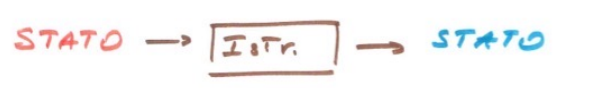
\includegraphics[scale=0.5]{images/cambio_stato.png}
\end{figure}

\paragraph{Esecuzione di un programma $P$ e sua semantica}
L'esecuzione di un programma consiste nell'esecuzione di molteplici cambiamenti di stato a partire
dallo stato iniziale $S_{init}$ (partendo un inpput $n$)
e giungendo a quello finale $S_{final}$. Si dice che la computazione
di $P$ induce una sequenza di stati.

\begin{figure}[H]
    \centering
    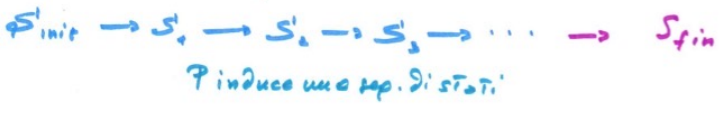
\includegraphics[scale=0.5]{images/stati_seq.png}
    \caption{Sequenza di stati indotta da $P$}
\end{figure}
\begin{figure}[H]
    \centering
    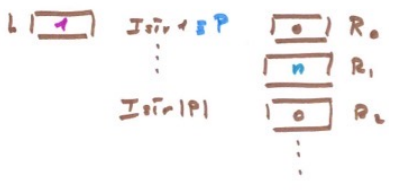
\includegraphics[scale=0.5]{images/stato_init.png}
    \caption{Situazione globale durante $S_{init}$}
\end{figure}
\begin{figure}[H]
    \centering
    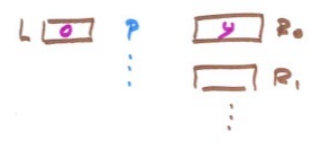
\includegraphics[scale=0.5]{images/stato_fina.png}
    \caption{Situazione globale durante $S_{final}$ (in caso di $HALT$)}
\end{figure}
Quindi la semantica del programma sarà:
\[
    \varphi_p(x) =
    \begin{cases}
        y \\
        \bot
    \end{cases}
\]
Dove $\bot$ mi indica una sequenza infinita di stati in loop.
\paragraph{Ingredienti della definizione formale della semantica}\mbox{}\\
\begin{itemize}
    \item \textbf{Stato} di una macchina RAM, è lo stato dei registri di quella macchina.
          Matematicamente modellato come una funzione che mi restituisce il contenuto
          del risultato quando la macchina è nello stato $S$
          $$S:\{L, R_i\}\rightarrow\mathbb{N}$$
          $$STATI=\mathbb{N}^{\{L,R_i\}}=\{\text{insieme di tutti i possibili stati della macchina}\}$$
          $$S(R_j) = \textit{contenuto di } R_j\text{ durante lo stato } S$$

    \item \textbf{Stato finale} della macchina RAM, uno stato tale per cui:$$S(L)=0\implies HALT$$
    \item \textbf{Dato}, rappresentato da $\mathbb{N}$, questo perchè sappiamo che $\mathbb{N}\sim DATI$.
    \item \textbf{Inizializzazione}, dato il dato $n$ prepara la macchina nello stato iniziale
          con input $n$. Quindi sarà una funzione $in$ questa creerà uno stato $S_{init}$ a partire
          da un input $n$:
          $$in:DATI\rightarrow STATI \text{ t.c. } in(n)=S_{init}$$
          Essa imposterà il contenuto del primo registro ad $1$, e tutti gli altri a $0$, e poi
          il caricherà nel program counter l'indirizzo della prima istruzione (contenuto
          del registro).
          \[
              S_{init}(R_i)=
              \begin{cases}
                  n & \text{se } i=1 \\
                  0 & \text{se } i=0
              \end{cases}
          \]
          $$S_{init}(L)=1$$

    \item \textbf{Programmi}, insieme dei programmi RAM $PROG=\{\text{programmi RAM}\}$, un
          singolo programma $P\in PROG$, tale per cui la sua cardinalità indica
          il numero di istruzioni contenute $|P| = \#istr$.
    \item \textbf{Esecuzione}, essa mi specifica la dinamica del programma che mi fa
          passare da uno stato al successivo. Questo è possibile con la \textit{funzione
              stato prossimo} $\delta$. Tale funzione mi permette di spostarmi dallo stato attuale
          $S$ a quello successivo $S'$.
          $$\delta:STATI\times PROG \rightarrow STATI_\bot$$
          $$\delta(S,P)=S'$$
          Lo stato prossimo dipenderà dall'istruzione che in quel momento deve essere eseguita,
          e per conoscere tale istruzione devo andare a vedere il contenuto del program counter
          allo stato attuale $S(L)$ (quindi lo stato prossimo dipenderà da $S(L)$).\\\textit{Come
              è definito lo stato prossimo in funzione dello stato attuale?}
          \begin{enumerate}
              \item Se $S(L)=0$ (ovvero in terminazione), allora lo stato prossimo non è definito
                    $S'=\bot$.
              \item Se $S(L)>|P|$, significa che abbiamo superato l'ultima istruzione
                    e che il program counter è stato incrementato diventando così più
                    grande del numero di istruzioni del programma. Quello che si fa è:
                    $$S'(L)=0\text{ HALT}$$
                    $$\forall i:S'(R_i)=S(R_i)$$
              \item Se $1\leq S(L)\leq |P|$, questo è il caso comune e considerando
                    la $S(L)$-esima istruzione:
                    \begin{itemize}
                        \item $R_k\leftarrow R_k \pm 1$, definite come:
                              \begin{lstlisting}[mathescape=true]
$S'(R_k) = S(R_k) \pm 1$
$S'(L)=S(L)+1$
$S'(R_i)=S(R_i)\text{ con } i\neq k$
                        \end{lstlisting}
                        \item $\text{IF }R_k=0\text{ THEN GOTO }m$, definita come:
                              \begin{lstlisting}[mathescape]
$S'(R_i) = S(R_i)$
if $S(R_k)==0$ then
    $S'(L)=m$
else
    $S'(L)=S(L)+1$
                        \end{lstlisting}
                    \end{itemize}
          \end{enumerate}
          \paragraph{Esecuzione del programma $P\in PROG$}\mbox{}\\
          Ora posso definire la sequenza di computazione di un programma $P\in PROG$ su un input $n\in\mathbb{N}$.
          Una computazione è una sequenza di stati indotta dalla dinamica:
          $$in(n)=S_0, S_1,...,S_i,S_{i+1},...$$
          Eventualmente la sequenza può essere infinita (loop), o terminare se un $S_m$
          raggiunge un $S_m(L)=0$ (halt).

          Dobbiamo vincolare la sequenza di stati alla funzione $\delta (S,P)$,
          e dire che per ogni $\delta(S_i,P)= S_{i+1}$.

          Quindi, la semantica di $P$, è definita come $\varphi_P:\mathbb{N}\rightarrow\mathbb{N}_\bot$:
          \[
              \varphi_P(n)=
              \begin{cases}
                  y    & \parbox[t]{.6\textwidth}{se la computazione del programma termina in con $S(L)=0$
                  ed il contenuto di $S_m(R_0)=y$}                                                        \\
                  \bot & \text{ se la computazione del programma va in loop}
              \end{cases}
          \]
\end{itemize}
Ora posso definire formalmente la potenza computazionale del sistema RAM:
$$F(RAM)=\{f\in\mathbb{N}^{\mathbb{N}}:\exists P\in PROG,\varphi_P = f\}=\{\varphi_P : P\in PROG\}\subsetneq\mathbb{N}^{\mathbb{N}}_{\bot}$$
Ovvero tutte le funzioni per cui esiste un programma $P$ tale per cui $\varphi_P = f$ (o $\varphi_P$ al variare di $P$).

\paragraph{Alcuni programmi RAM e le loro funzioni che vengono calcolate}\mbox{}
\begin{figure}[H]
    \centering
    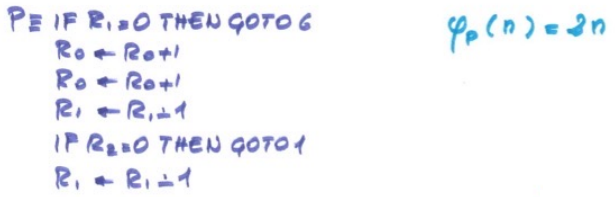
\includegraphics[scale=0.5]{images/2n.png}
    \caption{$n$}
\end{figure}

\begin{figure}[H]
    \centering
    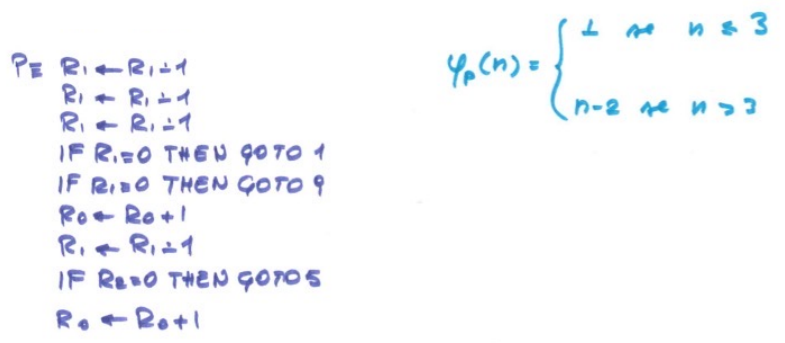
\includegraphics[scale=0.5]{images/n_complx.png}
    \caption{Funzione più complicata}
\end{figure}

Questi programmi possono essere spiegati formalmente con gli strumenti matematici precedentemente
forniti, per esempio con il primo programma:

\begin{figure}[H]
    \centering
    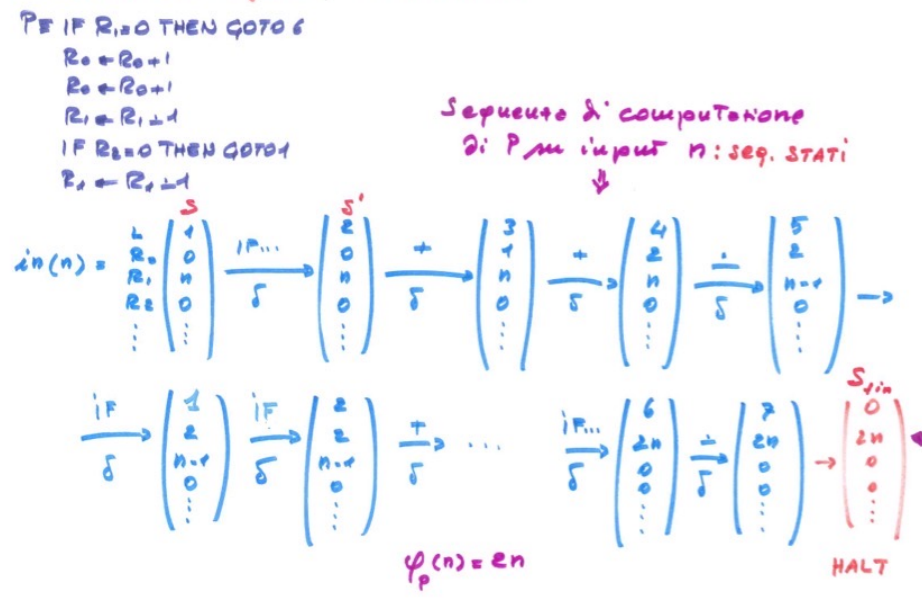
\includegraphics[scale=0.4]{images/n_formale.png}
    \caption{Rappresentazione formale di $\varphi_P(n)=2n$}
\end{figure}

Questo è il modo corretto di procedere, e questo modo permette di definire formalmente
la potenza computazionale di una macchina RAM, non lasciando nulla al caso.

\paragraph{Alcune considerazioni}
\begin{itemize}
    \item $F(RAM)$ \textit{conterrà funzioni più complesse o solo quelle banali?} In realtà
          si possono eseguire delle funzioni più complesse, questo comunque è un primo
          tentativo di fare qualcosa di ragionevole che mi permette la completa formalizzazione.
    \item Indubbiamente la semplicità di questo sistema di calcolo ci permette l'estrema
          formalizzazione, tale che vedremo che sarà possibile dimostrare $PROG\sim\mathbb{N}$
\end{itemize}

\subsubsection{Dimostrazione $PROG\sim\mathbb{N}$}
Dato un programma RAM vogliamo associare un numero a tale programma
in maniera che partendo quel numero sia possibile tornare al sorgente.

Ovvero vogliamo dimostrare che anche i programmi possono essere in corrispondenza biunivoca
con i numeri naturali (utilizzeremo la semplicità della macchina RAM).

$$P\equiv Istr_1,Istr_2,...,Istr_m$$
Il primo passo consiste nell'aritmetizzazione dell'istruzione, ovvero trasformare una lista
di istruzioni in una lista di codici numerici. Successivamente utilizzando la funzione lista
di Cantor possiamo trasformare questo elenco di codici in un singolo numero $n$.
\begin{figure}[H]
    \centering
    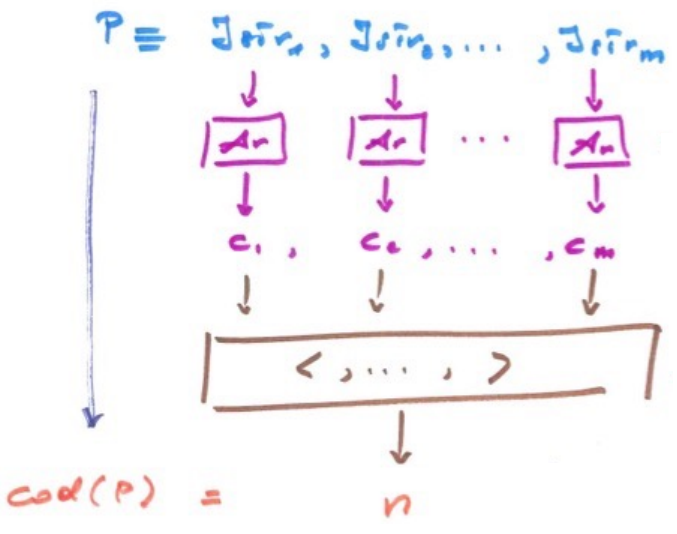
\includegraphics[scale=0.5]{images/PROG_to_num.png}
\end{figure}
Sappiamo che la funzione lista di Cantor è invertibile quindi possiamo ricostruire le codifiche
associate alle istruzioni. Ora se l'operazione di aritmetizzazione del sorgente è
invertibile, allora ci sarà possibile risalire al sorgente partendo da $n$.

In generale un procedimento che fa corrispondere ad una qualsiasi struttura matematica
un numero, si chiama operazione di \textbf{aritmetizzazione} o \textbf{Godelizzazione}.

Il nostro scopo è quello di aritmetizzare ogni istruzione.

\paragraph{Aritmetizzare biunivocamente le istruzioni RAM}
$$Ar:Istr\rightarrow\mathbb{N}\text{ e }Ar^{-1}:\mathbb{N}\rightarrow Istr\text{ t.c. }
    Ar(Istr)=n\Leftrightarrow Ar^{-1}(n)=Istr$$
Nel caso di un programma RAM significa aritmetizzare tre tipi di istruzioni.
$$Ar(R_n\leftarrow R_n+1)=3k$$
$$Ar(R_n\leftarrow R_n-1)=3k+1$$
$$Ar(\text{If }R_k=0\text{ then goto }m)=3\langle k,m\rangle-1$$
In questa maniera posso sapere da che registro proviene l'istruzione.
Come è fatta $Ar^{-1}$? La funzione di decodifica è biunivoca ? La funzione
risulta sia iniettiva che suriettiva, l'applicazione di questa funzione è permessa
attraverso l'operatore di modulo per $3$.
\begin{figure}[H]
    \centering
    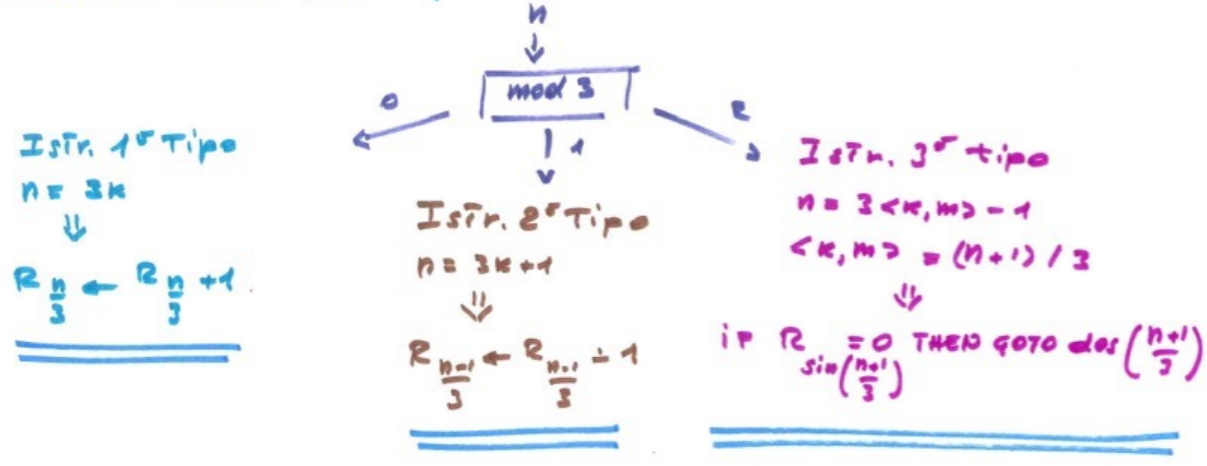
\includegraphics[scale=0.4]{images/mod3.png}
\end{figure}

Ricapitolando, il passaggio da programmi a numeri è molto semplice
$$cod(P)=\langle Ar(Istr_1),...,Ar(Istr_m)\rangle$$
mentre il passaggio da numeri a programmi, parto da $n$ e trovo la parte sinistra e
la parte destra. Vediamo passo per passo:

\begin{figure}[H]
    \centering
    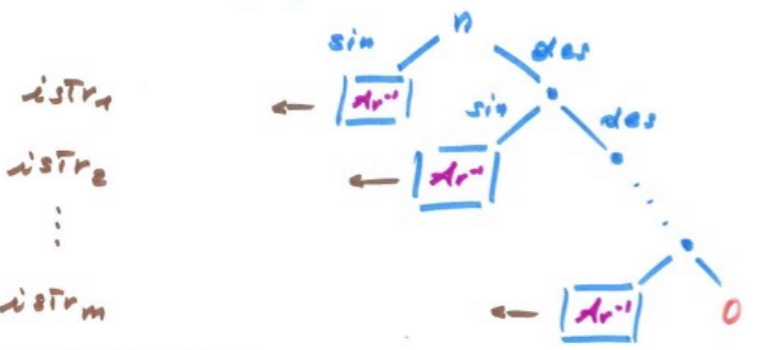
\includegraphics[scale=0.5]{images/decod_bin.png}
\end{figure}

Al primo passo dalla parte sinistra trovo il codice della prima istruzione
(aritmetizzato), quindi nel caso in cui io voglia il sorgente del programma
quello che devo fare è applicare $Ar^{-1}$ sulla parte sinistra. Questo finché
non si incontra il terminatore sul figlio destro.\\Se io volessi sempre
scompattare il programma $P$ e dato $n$ io volessi sapere il numero di istruzioni
del programma $|P|$, che cosa devo calcolare?
$$|P|=length(cod(P))$$
Abbiamo quindi dimostrato in maniera inequivocabile il secondo tassello, ovvero
che i programmi sono equinumerosi rispetto ai numeri naturali.
$$PROG\sim\mathbb{N}$$

Adesso che abbiamo acquisito gli strumenti, proviamo a vedere ad occhio qualche
esempio.

\paragraph{Primo programma RAM}\mbox{}\\
\begin{figure}[H]
    \centering
    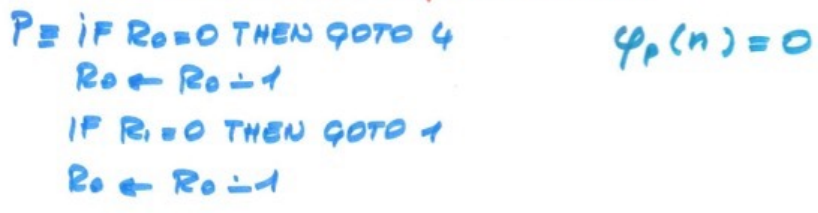
\includegraphics[scale=0.5]{images/prog_1.png}
\end{figure}

La corrispettiva aritmetizzazione delle istruzioni :

\begin{figure}[H]
    \centering
    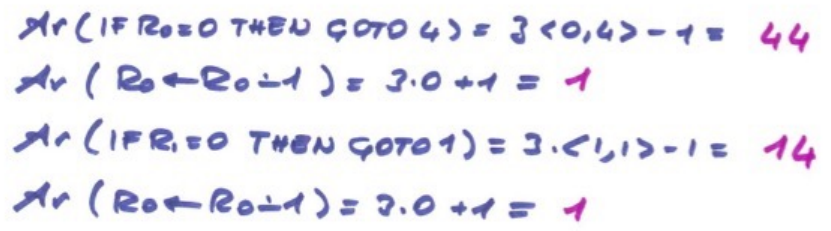
\includegraphics[scale=0.5]{images/cod_1.png}
\end{figure}
$$cod(P)=\langle 44,\langle 1,\langle 14,\langle 1,0\rangle\rangle\rangle\rangle=50556496$$
Questo non è un ottimo modo per compattare i programmi ram, poiché cresce esponenzialmente
rispetto al programma. Tuttavia questo ha scopi didattici.
$$\varphi_{50556496}(n)=0$$

\paragraph{Sorgente RAM da un numero}\mbox{}\\
Il numero è il 311, ha come parte sinistra 14 e come parte destra 10. Facendo il modulo 3
del figlio sinistro otteniamo otteniamo 2, quindi si tratta di un istruzione condizionale,
in questo caso troviamo che il valore della coppia di Cantor $\langle k,m\rangle = 5$. Quindi
dobbiamo trovare il figlio sinistro e destri di $5$, che sono entrambi $1$. Quindi
la prima istruzione sarà:
$$\text{If }R_1=0\text{ then goto }1$$
\begin{figure}[H]
    \centering
    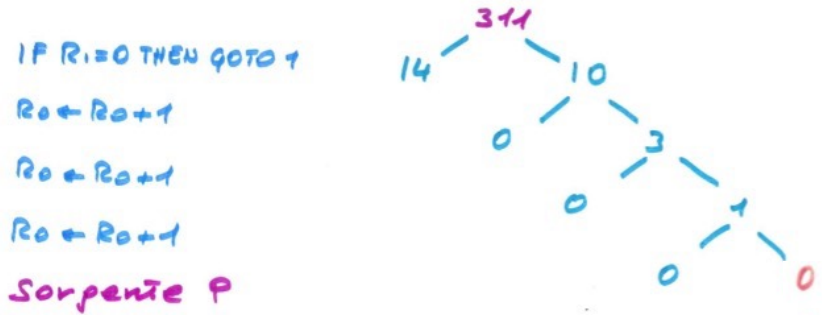
\includegraphics[scale=0.5]{images/sorgente_p.png}

\end{figure}
Quale é la semantica di questo programma ? (ovvero $\varphi_P(n)$)
\[
    \varphi_P(n)=\varphi_{311}(n)=
    \begin{cases}
        \bot & \text{se }n=0 \\
        3    & \text{se }n>0
    \end{cases}
\]
Se l'input $n$ è 0 vado in loop, poiché continuo a rieseguire la stessa istruzione,
altrimenti parto dalla terza istruzione.

\paragraph{Riflessioni su $PROG\sim\mathbb{N}$}
\begin{itemize}
    \item Abbiamo dimostrato che i numeri sono un linguaggio di programmazione, questo
          perché un numero può rappresentare un linguaggio.

    \item $F(RAM)=\{\varphi_P :P\in PROG\}$, la potenzia computazionale del sistema di programmazione
          RAM, adesso la posso scrivere come $F(RAM)=\{\varphi_i\}_{i\in\mathbb{N}}$ questo mostra ina maniera inequivocabile che la potenza
          computazionale della macchina RAM è enumerabile.

    \item Per il sistema RAM si ha rigorosamente che $F(RAM)\sim\mathbb{N}\nsim\mathbb{N}^{\mathbb{N}}$,

    \item Questa è una prima idea di calcolabilità, esploriamo un sistema di calcolo $\mathcal{C}$ più complesso
          e vediamo la sua potenza computazionale di questo, e vediamo se è più complessa. Questo va fatto è onestamente
          dire che ciò che è calcolabile sia $F(RAM)$ è troppo restrittivo.

    \item Possiamo avere che questo sistema di calcolo più avanzato ampli l'insieme $F(RAM)$.
\end{itemize}

\subsubsection{Il sistema di calcolo While}
Il linguaggio è basato su un linguaggio moderno, contrapposto all'assembly della macchina RAM (quindi
anni 50'), adesso ci troviamo nell'utilizzo di un linguaggio strutturato.

Hardware:
\begin{itemize}
    \item \textbf{Memoria} costituita da 21 registri. Siccome parliamo di linguaggio strutturato
          non si parla più con il termine registri ma ci si riferirà con \textit{variabili}.
          $$x_0,x_1,...,x_{20}$$. La variabile $x_1$ ci si troverà l'input del programma, mentre
          l'output si troverà su $x_0$.
    \item Program counter non presente, poiché si parla di linguaggio strutturato, ed in questo
          le istruzioni vengono eseguite una dopo l'altra (punti di inizio ciclo e finale
          sono ben definiti, ed il \textit{goto} non è presente).
\end{itemize}
20 variabili potrebbero sembrare poche, in realtà la numerosità dei dati non è un problema
poiché abbiamo primitive che mi permettono di condensare (coppia di Cantor) un infinità
di variabili.\\Il linguaggio while ha una sintassi induttiva (dove i costrutti dei linguaggi
sono definiti su delle basi semplici, i mattoni, e man mano costruisco istruzioni più
complesse):
\begin{itemize}
    \item Comando di \textbf{assegnamento}:
    $$x_k:=0$$
    $$x_k:=x_j+1$$
    $$x_k:=x_j-1$$
    \item Comando \textbf{while}: $\text{while }x_k\neq 0\text{ do } G$, dove $G$
          ovvero il corpo del loop, può essere un comando di assegnamento, while o composto.
    \item Comando \textbf{composto}: $\underline{\text{begin }}C_1; C_2; ...;C_m;
              \underline{\text{ end}}$ dove la sequenza è composta da comandi che possono essere
          di assegnamento, while o composto.
\end{itemize}
Come si può vedere sono strutture che sono in grado di nascondere altre strutture, di per sè
un programma WHILE è un comando composto.\\Indicheremo com $W-PROG=\{\text{programmi WHILE}\}$
come l'insieme dei programmi WHILE, dove ciascuno è un programma costruito induttivamente.

\paragraph{Esempio di programma WHILE}\mbox{}\\
\begin{figure}[H]
    \centering
    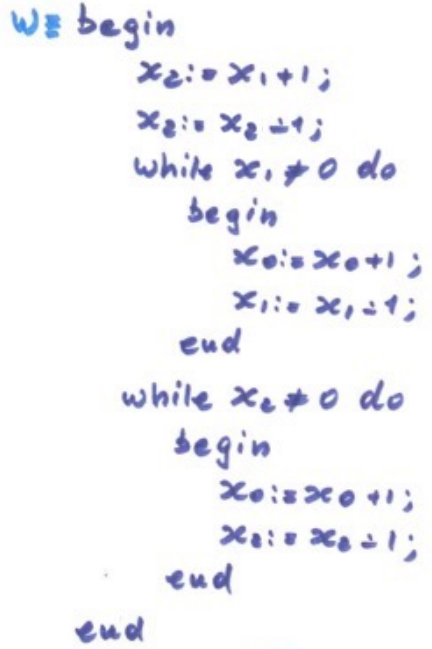
\includegraphics[scale=0.5]{images/esempio_prog_while.png}
\end{figure}
Indicheremo con $\psi_w$ le semantiche dei programmi WHILE (in questo caso il programma $w$).
$$\psi_w :\mathbb{N}\rightarrow\mathbb{N}_\bot$$
$$\psi_w (x)=2x$$

Le prime due istruzioni sono messe perché non è possibile effettuare una copia diretta,
non stiamo utilizzando il linguaggio di programmazione RAM.

Il parsing del programma ne rivela la struttura induttiva,
W-PROG è un insieme definito induttivamente (ovvero partendo
dalla base ed utilizzando dei passi induttivi): per dimostrare una proprietà $P$ su W-PROG:
\begin{enumerate}
    \item Dimostro che $P$ vale sui comandi base (passo base).

    \item Suppongo vero quella proprietà $P$ sui comandi $C$ base, e
          poi dimostro che vale sul comando più complesso $\text{while }x_n\neq 0\text{ do } C$
          (passo induttivo).

    \item Suppongo vera $P$ su $C_1,...,C_m$ e la dimostro vera su $\underline{\text{begin}}\text{ }
              C_1;...;C_m\text{ }\underline{\text{end}}$
\end{enumerate}

Quando abbiamo di fronte una struttura induttiva il modo migliore per dimostrare che una certa proprietà valaga su tutti
gli elementi della struttura dobbiamo farlo per induzione (in questo caso si parla di \textbf{induzione strutturale}).

\paragraph{Esempio}\mbox{}\\
L'insieme degli alberi binari è un insieme definito induttivamente. Sappiamo che è un DAG.
\begin{figure}[H]
    \centering
    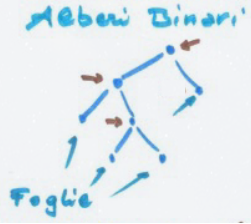
\includegraphics[scale=0.5]{images/BT.png}
    \label{fig:bt}
\end{figure}
Possiamo definire l'insieme degli alberi binari come l'insieme di tutti gli oggetti composti come
mostrato in figura \ref{fig:bt}. Oppure, possiamo definirli induttivamente

\begin{itemize}
    \item Base: Un nodo solo è considerabile un albero binario (con una singola foglia).
    \item Induzione: Se $T_1$ e $T_2$ sono alberi binari anche
          \begin{figure}[H]
              \centering
              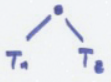
\includegraphics[scale=0.6]{images/BT_1.png}
              \caption{Binary Tree (indicati i nodi interni con le frecce marroni)}
          \end{figure}
    \item Nient'altro è un albero binario.
\end{itemize}
Allora vogliamo dimostrare pre induzione la proprietà $P$, tale che:
$$P\equiv \parbox[t]{.6\textwidth}{"Su ogni albero binario, il numero dei nodi interni è minore di uno rispetto
        a quello delle foglie."}$$

Allora dimostriamola per induzione:
\begin{itemize}
    \item Base: \textit{è vero che se ho un solo nodo la proprietà $P$ è vera?} Si poiché
          nodi interni non sono presenti.
    \item Induzione: supponiamo vera $P$ su $T_1,T_2$
          \begin{itemize}
              \item $T_1$: foglie $f_1$ foglie e $f_1-1$ nodi interni.
              \item $T_2$: foglie $f_2$ foglie e $f_2-1$ nodi interni.
          \end{itemize}

          Per esempio, prendiamo questo albero:
          \begin{figure}[H]
              \centering
              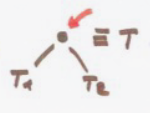
\includegraphics[scale=0.6]{images/BT_2.png}
          \end{figure}
          notiamo che il numero di foglie è pari a $f_1+f_2$. Adesso la domanda fondamentale è la seguente
          \textit{quanti nodi interni ha questo albero?} Il numero di nodi interni è pari alla somma tra i nodi
          interni di $T_1$ con quelli di $T_2$. Ma questo riutilizzando i mattoncini basilari non è altro che
          $$(f_1-1) + (f_2-1) + 1 = f_1 + f_2 -1$$
          $P$ risulta dimostrata per induzione su tutta la struttura.
\end{itemize}

\paragraph{Esempio 2}\mbox{}\\
Voglio definire una funzione $depth: \tau\rightarrow\mathbb{N}$ su un albero binario che
dato un qualsiasi albero binario mi restituisce la \textbf{profondità}: ovvero, la lunghezza del
cammino più lungo dalla radice ad una foglia dell'albero.
\begin{figure}[H]
    \centering
    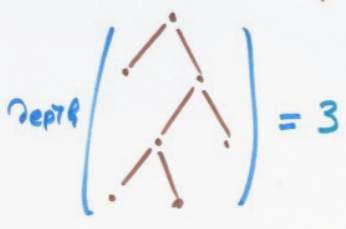
\includegraphics[scale=0.6]{images/profondità.png}
    \caption{Definizione grafica}
\end{figure}
Questa è una possibile definizione, oppure potremmo definirla induttivamente:
\begin{enumerate}
    \item Base: Dato un BT costituito da una sola radice darà $depth=0$
    \item Induzione: Dato questo albero binario
          \begin{figure}[H]
              \centering
              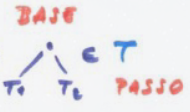
\includegraphics[scale=0.6]{images/passo_ind_depth.png}
          \end{figure}
          si prende la profondità maggiore due due sotto alberi più uno, ovvero il nuovo livello
          $depth=1+max\{depth(T_1),depth(T_2)\}$
    \item Nient'altro è in $\tau$
\end{enumerate}

\paragraph{Esecuzione su una macchina WHILE}\mbox{}\\
Considerando un input $n$
\begin{itemize}
    \item La prima è una fase di inizializzazione, quindi si avvia la macchina con il nostro
          programma $w$, dove tutte i registri della variabili sono inizializzati a 0, tranne per il registro
          in input $x_1$ che contiene $n$.

    \item Si comincia ad eseguire il programma $w$, sequenzialmente sulle istruzioni, in questo caso non
          c'è assolutamente bisogno di program counter (motivi già spiegati).

    \item Possiamo avere due casi, o l'esecuzione effettivamente termina o si incappa in un loop (while true).
          Nel primo caso l'output lo andiamo a leggere nella variabile $x_0$ (se HALT), altrimenti diciamo che è indefinito
          $\bot$. Definendo così la semantica del programma $w$, $\psi_w(n)=cont(x_0)/\bot$.
\end{itemize}

Vogliamo essere precisi anche in questo caso, ed espandere il discorso della sequenza di istruzioni durante l'esecuzione
di un programma WHILE (introducendo anche qui il concetto di stato).

\subsubsection{Definizione formale di semantica di un programma WHILE}
\begin{itemize}
    \item \textbf{Stato}, una foto dove compare in maniera completa tutto ciò che accade sulla macchina in quel dato istante.
          Rispetto alla macchina RAM lo stato viene definito in maniera differente, dal punto di vista matematico uno stato è
          una tupla di 21 elementi $(c_0, ..., c_{20})$. Detto ciò, l'insieme di tutti i possibili stati $w-stati$ è composto
          da $\mathbb{N}^{21}$ ovvero tutte le possibili 21-tuple (tuple di lunghezza 21) infinite.

    \item \textbf{Dati}, sono l'insieme dei numeri naturali.
    \item \textbf{Inizializzazione}, sta volta la funzione può essere modellata su 21 elementi, la funzione prende un
          numero e restituisce uno stato
          $$W-in:\mathbb{N}\rightarrow\mathbb{N}^{21}\text{ con }W-in(n)=(0,n,0,...,0)$$
    \item \textbf{Semantica operazionale}
          $$[]():W-COM\times W-STATI\rightarrow W-STATI_\bot$$
          Dato un comando while $C$ e uno stato $\underline{x}$, allora
          $$[C](\underline{x})=\underline{y}$$
          sarà la funzione stato prossimo dove $\underline{y}$ è lo stato prossimo di $\underline{x}$ a seguito
          dall'esecuzione del comando $C$.
          Ovviamente possiamo definire induttivamente $[C](\underline{x})$ sulla struttura induttiva
          del comando $C$.
\end{itemize}

\subsubsection{Definizione induttiva della semantica while}
\begin{itemize}
    \item Base: gli \textbf{assegnamenti}
          \[
              [x_k:=0](\underline{x})=\underline{y}\text{ con }y_i=
              \begin{cases}
                  x_i & \text{se }i\neq k \\
                  0   & \text{se }i=k
              \end{cases}
          \]

          \[
              [x_k:=x_j \pm 1](\underline{x})=\underline{y}\text{ con }y_i=
              \begin{cases}
                  x_i       & \text{se } i\neq k \\
                  x_j \pm 1 & \text{se } i=k
              \end{cases}
          \]
Queste sempre considerando l'operatore di $\dot{-}$.
    \item Passo:
          \begin{itemize}
              \item Comando \textbf{composto}
                    $$[\underline{\text{begin}}\;C_1;...;C_m;\underline{\text{end}}](\underline{x})$$
                    induttivamente conosco la semantica di ciascuno di questi programmi, come essi agiscono.
                    Allora posso definire la semantica di questo comando come:

                    $$[C_m](\dots([C_2]([C_1](\underline{x})))\dots)=\underline{y}=[C_1]\circ \dots\circ [C_m](\underline{x})$$
                    Quindi l'applicazione del primo comando (che provoca cambiamento di stato)
                    sullo stato iniziale, seguita iterativamente dall'applicazione di $m$ comandi
                    sugli stati risultanti.

              \item Comando \textbf{while}
                    $$[\text{while }x_k\neq 0 \text{ do }C](\underline{x})$$
                    anche qui conosco per ipotesi induttiva la semantica del comando $C$.

                    $$[C](\dots([C]([C](\underline{x})))\dots)=\underline{y}=[C_1]\circ\dots\circ[C_m](\underline{x})$$
                    Il numero di volte che applicherò il comando $C$ quante volte serve per azzerare il contenuto di $x_k$
                    \[
                        =
                        \begin{cases}
                            [C]^e(\underline{x}) & \text{con }e=\mu t :\text{la}\;k\text{-esima componente di }[C]^{(t)}(\underline{k})=0 \\
                            \bot                 & \text{altrimenti}
                        \end{cases}
                    \]
                    Ovvero il più piccolo numero di volte (la più piccola $t$, dove $t$ è l'iterazione) che mi serve
                    per azzerare la componente $k$-esima, altrimenti vado in un loop interminabile.
          \end{itemize}
\end{itemize}

\paragraph{Semantica di $W$ e $W-PROG$}\mbox{}\\
A questo punto so definire in maniera formale la semantica
di un programma while, prendiamo il programma WHILE $w$ (il quale è un comando composto).

Quindi è la semantica del comando composto che rappresenta $w$, quindi non è altro che preparare
la macchina su input $x$.

$$\Psi_w(x)=Pro(0,[w](W-in(x)))$$
Ovvero la proiezione $0$-esima dell'esecuzione del comando composto di $w$ dato uno stato finale $x$ (avviato
da uno stato iniziale),
significa che se il programma termina devo pescare il contenuto di $x_0$ (la proiezione di uno stato finale
di un programma $w$).
Nel caso in cui non avvenisse l'HALT allora avrò una semantica indefinita $\bot$.

\paragraph{Esempio di semantica di un piccolo programma while}\mbox{}\\
\begin{figure}[H]
    \centering
    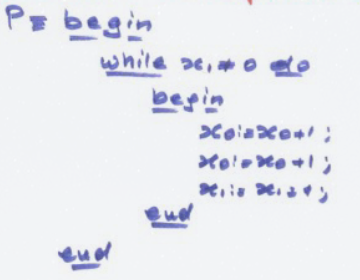
\includegraphics[scale=0.7]{images/smallprog.png}
    \caption{Programma che calcola $2n$}
\end{figure}

\begin{figure}[H]
    \centering
    \includegraphics[scale=0.7]{images/comanodwhiòe.png}
    \caption{Deduzione della semantica $\Psi_w$}
\end{figure}

\paragraph{Potenza computazionale del sistema WHILE}\mbox{}\\
$$F(WHILE)=\{f\in\mathbb{N}_\bot^\mathbb{N} : \exists w\in W-PROG, f=\Psi_w\}=\{\Psi_w : w\in W-PROG\}$$
Definiamo la potenza computazionale di
una macchina WHILE come l'insieme di tutte le funzioni per cui
esiste un programma WHILE per cui si può calcolare quella funzione.
Naturalmente la domanda è: \textit{che relazione esiste tra $F(RAM)$ e -$F(WHILE)$?}, quindi
che cosa è calcolabile di questi due sistemi? $\{\varphi_P:P\in PROG\}$?
Magari la macchina WHILE mi fornisce più potenza della macchina RAM? L'unico modo di scoprirlo
è confrontando le due idee. Quali situazioni si possono verificare:
\begin{enumerate}
    \item Una situazione dove $F(RAM)\subsetneq F(WHILE)$ (inclusione propria) ovvero, che ci sono funzioni
          calcolabili con i programmi WHILE che non sono calcolabili sulle macchine RAM.

    \item Le due idee di calcolabilità non sono confrontabili, ovvero un intersezione tra i due insiemi
          dove magari alcune funzioni sono calcolabili da entrambe le architetture, oppure sono due insiemi
          totalmente disgiunti. In entrambi i casi siamo preoccupati, perché l'idea di calcolabilità è dipendente
          dal modello di calcolo adottato.

    \item Una situazione dove $F(WHILE)\subsetneq F(RAM)$ questo sarebbe sorprendente, la macchina
          sofisticata non riesce a calcolare delle funzioni più semplici.

    \item Una situazione dove $F(WHILE)=F(RAM)$, ovvero due cose filosoficamente diverse eppure entrambe
          riescono a calcolare la stessa classe di funzioni, questo sarebbe molto interessante, perché allora
          vuol dire che calcolabile non dipende dalla tecnologia.
\end{enumerate}
Adesso dobbiamo cercare di capire quali tra i seguenti punti è quello veritiero.

\paragraph{Confrontiamo $F(RAM)$ e $F(WHILE)$}\mbox{}\\
Iniziamo con il confrontare $F(RAM)$ e $F(WHILE)$ introducendo due sistemi di calcolo $\mathcal{C}_1$ e $\mathcal{C}_2$
con i loro relativi linguaggi di programmazione. Attraverso i quali riusciamo a scrivere l'insieme dei
programmi scritti con i relativi linguaggi $\mathcal{C}_1-PROG$ e $\mathcal{C}_2-PROG$. Le relative
potenze computazionali:

$$F(\mathcal{C}_1)=\{f\in\mathbb{N}_\bot^\mathbb{N}: f=\Psi_{P_1}\text{ per qualche }P_1\in\mathcal{C}_1-PROG\}=$$
$$=\{\Psi_{P_1}:P_1\in\mathcal{C}_1-PROG\}$$
$$F(\mathcal{C}_2)=\{f\in\mathbb{N}_\bot^\mathbb{N}: f=\varphi_{P_2}\text{ per qualche }P_2\in\mathcal{C}_2-PROG\}=$$
$$=\{\varphi_{P_2}:P_2\in\mathcal{C}_2-PROG\}$$
Cominciamo a cercare degli strumenti per confrontare le potenze computazionali. Come faccio a dimostrare
$F(\mathcal{C}_1)\subseteq F(\mathcal{C}_2)$
Per dimostrare che tale inclusione sia vera, mi basta dimostrare che un elemento di un insieme appartenga
all'altro, in linguaggio matematico:
$$\forall f\in F(\mathcal{C}_1)\implies f\in F(\mathcal{C}_2)$$
Quando stiamo compilando un programma quello che stiamo dimostrando è che il linguaggio utilizzato
come sorgente è potente uguale al linguaggio macchina (o oggetto).
$$\exists P_1\in\mathcal{C}_1-PROG : f=\Psi_{P_1}\implies\exists P_2\in\mathcal{C}_2-PROG:f=\varphi_{P_2}$$
Ovvero vuol dire che esiste un programma $P_1$ tale per cui ne esiste uno equivalente nel secondo
sistema (allora ho dimostrato che tutto ciò che è fattibile in $\mathcal{C}_1$ è fattibile in $\mathcal{C}_2$,
questo attraverso una \textit{traduzione}).

\subsubsection{Concetto di traduzione}
Dati i sistemi $\mathcal{C}_1,\mathcal{C}_2$, una \textbf{traduzione} (controparte di \textit{compilazione}) dal primo verso il secondo è
una funzione:
$$T:\mathcal{C}_1-PROG\rightarrow\mathcal{C}_2-PROG$$
con le seguenti proprietà (che sono quelle che vogliamo nei nostri compilatori):
\begin{itemize}
    \item deve essere \textbf{programmabile} effettivamente.
    \item deve essere \textbf{completa}, ovvero che traduce \textit{ogni} programma scritto in $\mathcal{C}_1$ in
          uno scritto in $\mathcal{C}_2$.
    \item deve essere \textbf{corretta}, ovvero che mantiene la semantica del programma
          $$\forall P\in\mathcal{C}_1-PROG :\varphi_{T(P)}=\Psi_P$$
\end{itemize}
questa è la formalizzazione del concetto di compilatore. Allora il \textbf{teorema} che posso scrivere
è il seguente, se esiste $T:\mathcal{C}_1-PROG\rightarrow\mathcal{C}_2-PROG$, allora $F(\mathcal{C}_1)\subseteq F(\mathcal{C}_2)$
se esiste una traduzione da $\mathcal{C}_1$ a $\mathcal{C}_2$, allora ho dimostrato che la potenza computazionale del
primo linguaggio è contenuto (o uguale) a quella del secondo.

\paragraph{Dimostrazione}\mbox{}\\
$$f\in F(\mathcal{C}_1)\implies\exists P\in\mathcal{C}_1-PROG:f=\Psi_P$$
$$\text{Applico } T \text{ ed ottengo}$$
$$T(P)\in\mathcal{C}_2-PROG\text{ (completa) con }\varphi_{T(P)}=\Psi_P=f$$
allora esiste dunque un programma $T(P)\in\mathcal{C}_2-PROG$ per $f$ per cui
$f\in F(\mathcal{C}_2)$.

Sostanzialmente, ipotizzo l'esistenza di una funzione che rientri nella potenza computazionale
del primo linguaggio $\mathcal{C}_1$,
esiste un programma $P$ scritto in questo linguaggio che è in grado di calcolare $f$.
Siccome esiste la traduzione, prendo $P$ e lo compilo, e questo funziona perché la traduzione è completa.

\subsubsection{Dimostrazine $F(WHILE)\subseteq F(RAM)$}
Da un punto di vista immediato sembrerebbe la cosa più difficile da dimostrare, ma se ci si pensa
è proprio quello che accade durante la compilazione dei programmi (per esempio C, C++,...).
Quindi vogliamo a dimostrare che la macchina RAM non ha nulla da invidiare rispetto alla macchina WHILE.

Dimostrare questa inclusione mi spinge ad esibire che esiste una traduzione da un programma WHILE ad
uno RAM
$$Comp:W-PROG\rightarrow PROG$$
Chiamerò questa traduzione \textit{compilazione} (la quale è una funzione di traduzione che
rispetta le tre proprietà). Per pura comodità, scrivere un compilatore da un programma WHILE ad uno
RAM vuol dire prendere un programma del primo tipo e scrivere un frammento del secondo, per semplicità
ammetterò di utilizzare un programma RAM che utilizza delle \textit{label} (cosa che mi permette
di fare salti nel codice).

\begin{figure}[H]
    \centering
    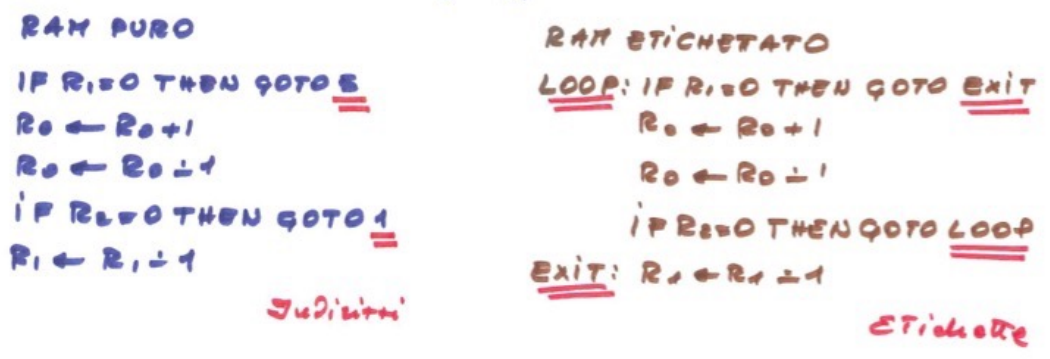
\includegraphics[scale=0.4]{images/ram_etichettato.png}
\end{figure}

semplicemente al posto di utilizzare i riferimenti numerici alle righe utilizzeremo delle parole,
con un semplice post-processing posso trasformare il "RAM etichettato" in "RAM puro" (l'aggiunta
di etichette non aumenta la potenza del linguaggio RAM).

\paragraph{Forma del compilatore}\mbox{}\\
Teniamo conto della natura degli oggetti su cui agirà il compilatore $W-PROG$ è un insieme definito
induttivamente. Questo significa che anche $Comp$ può essere definito induttivamente.

\begin{enumerate}
    \item mostriamo come compilare le basi di quel linguaggio, quindi gli assegnamenti (base).
    \item posso usare l'ipotesi induttiva, quindi assumo di saper compilare il comando $Comp(C_1),\dots,Comp(C_m)$ e ti
          faccio vedere come compilare il comando composto
          $$\underline{\text{begin}}\;C_1;\dots ;C_m; \underline{\text{end}}$$
    \item posso usare l'ipotesi induttiva, quindi di saper compilare $Comp(C)$ e mostrarlo come compilare il comando
          $while$ che ha come corpo $C$, $\underline{\text{while}}\;x_n\neq 0\;\underline{\text{do}}\;C$
\end{enumerate}

In tale maniera si saprà come compilare tutto $W-PROG$. Sia nota la seguente proprietà di compilazione,
ogni volta che durante una traduzione incontreremo nel programma una variabile $x_k$ ad essa verrà
associata il registro $R_k$ (abbiamo tranquillamente lo spazio per mappare tutte le variabili, visto
che il numero di registri è infinito).

\paragraph{Base: assegnamenti}\mbox{}\\
Vogliamo considerare i seguenti frammenti RAM per eseguire gli assegnamenti base dei programmi WHILE:
\begin{itemize}
    \item $Comp(x_k:=0)$
          \begin{figure}[H]
              \centering
              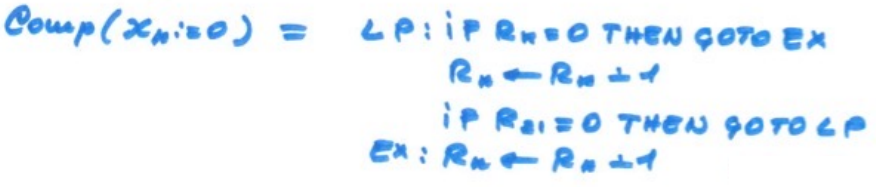
\includegraphics[scale=0.4]{images/assegnamento_ram.png}
          \end{figure}
          controllo se un registro è azzerato, nel caso non fosse azzerato allora lo decremento
          e ripeto il controllo ($R_{21}$ non sarà mai azzerato). Ad un certo punto uscirò dal ciclo,
          l'ultima operazione è praticamente nulla perché non danneggia l'operato precedente (è già zero).
          Tutti i registri da $R_{21}$ in poi sono tutti azzerati, perché non vengono utilizzati dal programma
          WHILE, quindi possiamo utilizzarli come meglio crediamo.

    \item $Comp(x_k:=x_j\pm 1)$

          notiamo che c'è un caso dove la compilazione è immediata, in un caso di quest'istruzione
          troviamo subito l'istruzione RAM che fa la stessa cosa. Il caso particolare accade quando
          $k=j$. Se $k==j\rightarrow R_k\leftarrow R_k\pm 1$, il problema allora è nell'altro caso,
          ovvero quando $k\neq j$.

          \begin{figure}[H]
              \centering
              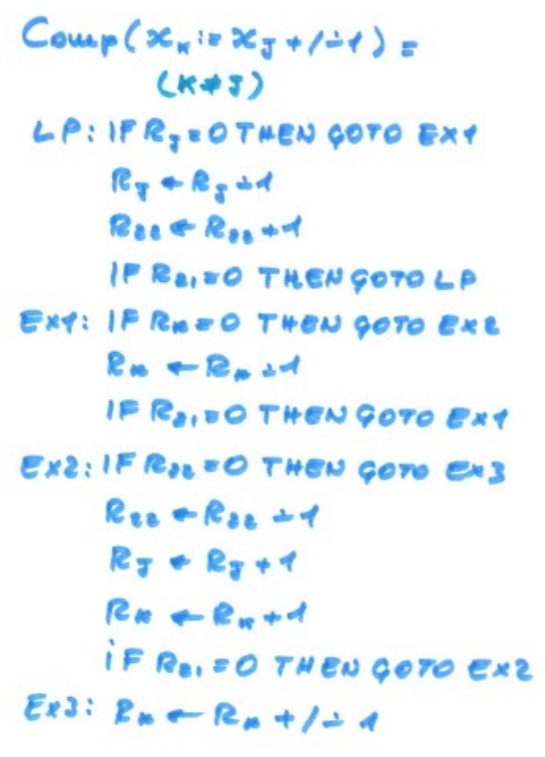
\includegraphics[scale=0.4]{images/assegnamento_ram2.png}
          \end{figure}
          \begin{enumerate}
              \item Salvo $x_j$ in $R_{22}$, questo attraverso le prime quattro istruzioni che seguono
              dall'etichetta $LP$.
              \item Azzero $x_k$, ovvero $R_k$ (etichetta $EX1$).
              \item Rigenero $x_j$ e $x_k$ da $R_{22}$ (etichetta $EX2$).
              \item Sommo/sottraggo 1 da $x_k$ (etichetta $EX3$).
          \end{enumerate}

          \paragraph{Passo induttivo}\mbox{}\\
          Consideriamo il comando composto $\underline{\text{begin}}\;C_1;...;C_m;\;\underline{\text{end}}$,
          considerando che esiste l'ipotesi induttiva, quindi assumo noti $Comp(C_1),\dots ,Comp(C_m)$
          mostro che la compilazione $Comp(\underline{\text{begin}}\;C_1;\dots;C_m\;\underline{\text{end}})$
          sarà:
          $$Comp(C_1);$$
          $$Comp(C_2);$$
          $$\dots$$
          $$Comp(C_m);$$

          Consideriamo il comando $\underline{\text{while}}\;x_k\neq 0\;\underline{\text{do}}\; C$,
          allora vogliamo mostrare che la compilazione $Comp(\underline{\text{while}}\;x_k\neq 0\;\underline{\text{do}}\; C)$
          corrisponde al frammento RAM:
          \begin{figure}[H]
              \centering
              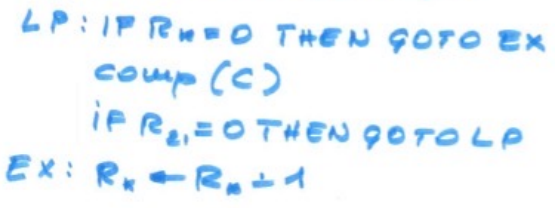
\includegraphics[scale=0.5]{images/comandowhile_ram.png}
          \end{figure}

          \paragraph{Ricapitolando}\mbox{}\\
          La funzione $Comp:W-PROG\rightarrow PROG$ che abbiamo definito induttivamente soddisfa:
          \begin{enumerate}
              \item è facilmente \textbf{programmabile}.
              \item compila ogni sorgente WHILE (\textbf{completo}).
              \item mantiene la semantica $\Psi_w=\varphi_{Comp(w)}\implies\textbf{ corretta}$
          \end{enumerate}
          I punti 2 e 3 si dimostrano facilmente per induzione strutturale, quindi possiamo dimostrare
          che $Comp$ è una traduzione da WHILE a RAM, e che quindi $F(WHILE)\subseteq F(RAM)$

\end{itemize}

\subsubsection{Dimostrazione $F(RAM)\subseteq F(WHILE)$}
Il problema in questo caso è dato dal fatto che si deve gestire l'operazione di "go to", che non
è presente nel linguaggio WHILE (ed è proprio per questo motivo che utilizzare
"go to" nei linguaggi strutturati è un problema). Dimostreremo come è possibile evitare l'utilizzo
delle istruzioni "go to" nella programmazione strutturata.

Introduciamo il concetto di \textbf{interprete}, per quasi tutti i linguaggi di programmazione
ormai c'è la possibilità di avere la versione compilata che interpretata
(con differenze prestazionali).
La compilazione produce un programma equivalente che sta in piedi da solo (\textit{stand-alone})
che può essere eseguito direttamente dalla macchina, l'interpretazione simula l'esecuzione
di un programma attraverso un interprete.

Vediamo come scrivere un interprete di programmi RAM scritto in WHILE, che chiameremo $I_W$.

\begin{figure}[H]
    \centering
    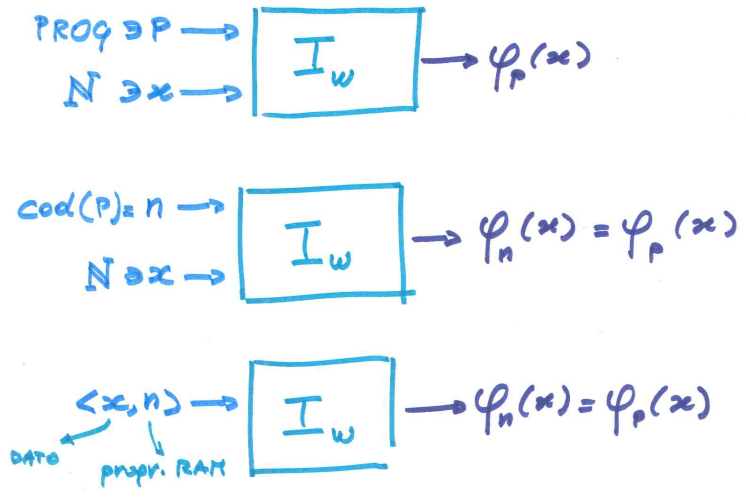
\includegraphics[scale=0.5]{images/interprete_while.png}
\end{figure}
Esso prenderà in ingresso un programma scritto in RAM ed un input, e produrrà in uscita
non un codice oggetto ma la semantica del programma $P$ sul dato $x$. Notiamo che in ingresso
viene dato un programma $P$ che è listato, ma sappiamo che i nostri programmi WHILE non lavorano
sulle stringhe. Un programma WHILE ha una sola variabile di input $x_1$ che può solo contenere
numeri. \textit{Come facciamo a fornire il listato di $P$ al programma WHILE?} Il mio $I_W$
prenderà in ingresso la codifica del programma $P$ che sarà fornita sotto forma di numero.

\textit{Ma il nostro programma può veramente prendere due dati in questa maniera?} Notiamo bene
che nel linguaggio WHILE $x_1$ non può prendere una coppia di numeri distinti, ma allora
dobbiamo passare un ulteriore coppia di Cantor di questi due numeri.

Il risultato sarà il funzionamento del programma con codice $n$ che in realtà è $P$.

Quindi la semantica di $I_W$:
$$\forall x,n\in\mathbb{N}:\Psi_{I_W}(\langle x,n\rangle)=\varphi_n(x)=\varphi_P(x)$$

\paragraph{Macro-WHILE}\mbox{}\\
Siccome devo scrivere un interprete in WHILE, voglio facilitarmi il lavoro utilizzando una
versione modificata del linguaggio (sempre permettendo di tornare al WHILE puro e senza
avere guadagni o perdite prestazionali). Questo per permettere di scrivere un codice
più semplice.

Per esempio:
\begin{figure}[H]
    \centering
    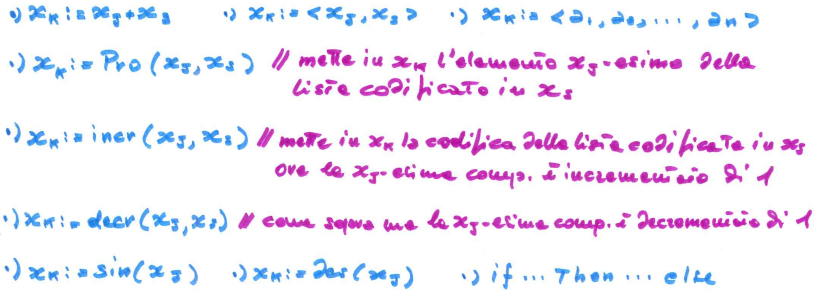
\includegraphics[scale=0.5]{images/macro-while.png}
\end{figure}

Come vediamo queste non sono istruzioni di WHILE puro, dovremmo scrivere molte più istruzioni
per ottenere ciò. Si ha anche la possibilità di rappresentare la coppia di Cantor di due numeri,
visto che si ottengono con somme/sottrazioni, ed anche la possibilità di rappresentare la
lista di Cantor.

Ciascuna di queste MACRO può essere sostituita da un frammento di WHILE puro (seppur risulti piò comodo
da utilizzare)
$$F(MACRO-WHILE)=F(WHILE)$$

\paragraph{Interprete WHILE di programmi RAM}\mbox{}\\
Lo scopo di questo interprete è quello di ricreare esattamente al suo interno (scritto
in WHILE) utilizzando le variabili la situazione della macchina RAM, entro cui fare
eseguire il programma.

Sappiamo che la macchina RAM riceve un programma $P$ che è un listato delle istruzioni di un programma
RAM. Sappiamo che la memoria della macchina RAM ha un numero infinito di registri
(a destra) ed un registro $L$ che è il program counter.
\begin{figure}[H]
    \centering
    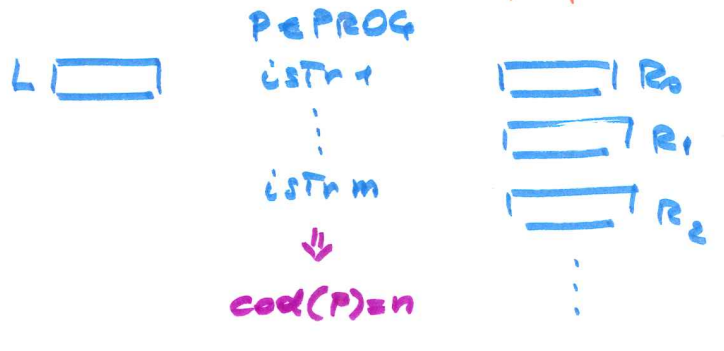
\includegraphics[scale=0.5]{images/interprete_while_ram.png}
\end{figure}
Questo interprete scritto in WHILE si trova davanti ad un problema iniziale, si ha un
numero di registri \textit{infinito} sulla macchina RAM (mi servono quindi un
numero infinito di variabili, ma purtroppo sono solo 21). Però sappiamo che il
nostro programma $P$ ha come codifica il numero $n$, allora sicuramente non userà
mai un registro il cui numero sarà superiore ad $n$, quindi $R_j<n$. Significa
che posso limitarmi a maneggiare un numero di registri che va da $R_0,\dots,R_{n+2}$,
quindi potrò sviluppare questa dinamica in una lista.

Utilizzo delle variabili da parte dell'interprete:
\begin{itemize}
    \item $x_0$ per indicare la porzione di \textbf{memoria della macchina} RAM
          che identifica i registri del programma, quindi lo stato della memoria istante
          per istante del programma che devo simulare.
    \item $x_1$ giocherà il ruolo del \textbf{program counter} $L$.
    \item $x_2$ metterò il dato su cui deve girare il programma (\textbf{input}).
    \item $x_3$ ci metterò il \textbf{listato del programma} ovvero $n$ (ovvero $cod(p)$).
    \item $x_4$ di volta in volta verrà caricata l'istruzione che il
          program counter deve eseguire (gioca il ruolo del registro di istruzione
          corrente \textit{instruction register}, IR).
\end{itemize}
è opportuno ricordare che inizialmente $I_w$ troverà il suo input nella variabile
$x_1$, ovvero $\langle x,n\rangle$, nella variabile input $x_1$:
\begin{figure}[H]
    \centering
    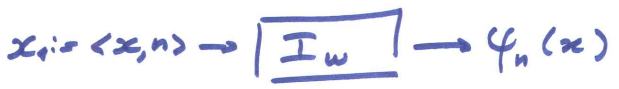
\includegraphics[scale=0.5]{images/x_1.png}
\end{figure}
Composizione dell'interprete:
$$I_W(\langle x,n\rangle)=\varphi_n(x)$$
\begin{figure}[H]
    \centering
    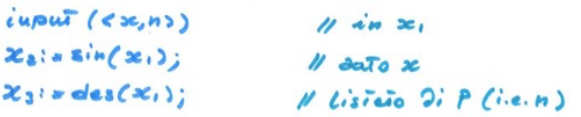
\includegraphics[scale=0.5]{images/inter_0.png}
\end{figure}
Rispettivamente i primi due registri $x_2$ ed $x_3$ vengono definiti facilmente, poiché
l'input del programma ed il listato si trovano sono rispettivamente il figlio sinistro
ed il figlio destro.
\begin{figure}[H]
    \centering
    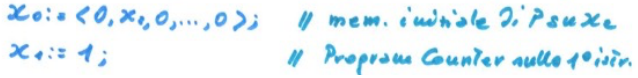
\includegraphics[scale=0.5]{images/inter_1.png}
\end{figure}
La variabile $x_0$ deve contenere la memoria del programma $P$, sappiamo che sarà
costituita dalla lista di tutti i registri che vanno da $R_0$ a $R_{n+2}$, dove in
$R_1$ sarà presente l'input del programma $P$ (che andremo a prelevare da $x_2$),
tutti i restanti registri saranno azzerati (la lista è ovviamente rappresentata
da una coppia di Cantor). Il program counter viene impostato all'inizio del programma
ad 1, in maniera che punti alla prima istruzione del programma.
\begin{figure}[H]
    \centering
    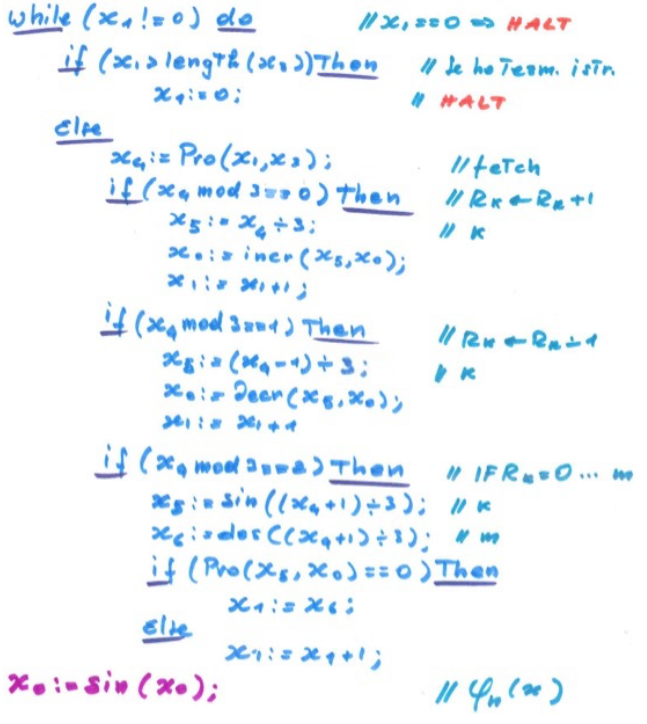
\includegraphics[scale=0.5]{images/fetch_decode_execute.png}
    \caption{Fetch - Decode - Execute}
\end{figure}
\begin{itemize}
    \item L'esecuzione di un programma RAM si ferma quando il program counter $L=0$ (HALT),
          l'interprete non è altro che un ciclo che esegue sempre le operazioni di
          fetch,decode e execute del processore.
    \item Sappiamo che l'interpretazione di un programma termina nel caso in cui
          abbiamo terminato la simulazione ci dobbiamo fermare, sappiamo che questo
          accade quando il program counter supera il numero di istruzioni. Il numero di
          istruzioni è condensato nella variabile $x_3$ , al superamento della dimensione
          di quest'ultima da parte di $x_1$, impostiamo l'HALT (altrimenti continuiamo
          con l'esecuzione del programma).
    \item Usiamo la macro $Pro()$ per prendere la codifica dell'istruzione del programma
          caricato in $x_3$ che viene puntato da $x_1$ e la carichiamo in $x_4$ (fetch).
    \item Si deve capire che tipo di istruzione stiamo trattando, questo lo possiamo
          fare considerando il resto della divisione per 3:
          \begin{itemize}
              \item Resto = 0, si tratta di un incremento di un registro $R_k$,
                    dove $k=x_4/3$. Questo significa andare nella memoria simulata in $x_0$, posizionarsi
                    nel registro $x_4/3$ ed incrementarlo di 1. Per sapere la posizione di $k$ utilizzo
                    una delle variabili disponibili, $x_5$, utilizzo la macro $Incr()$ per incrementare
                    l'elemento in posizione $x_5$ della lista $x_0$ (memoria del programma). Al termine avanzo
                    il program counter perché ho eseguito l'istruzione.
              \item Resto = 1, si tratta di un decremento di un registro $R_k$, in questo caso
                    il valore di $k=x_4-1/3$, la macro che utilizzo è $Decr()$ (per il resto come prima).
              \item Resto = 2, si tratta di un condizionale, allora devo trovare sia il $R_k$ (la condizione)
                    che $m$ (l'istruzione da eseguire). Una volta individuate si va a cercare l'istruzione
                    $m$ nella memoria della macchina, se presente si sposta il program counter a quell'istruzione,
                    altrimenti si continua linearmente con l'istruzione successiva.
          \end{itemize}
    \item Si carica nella variabile di output $x_0$ l'output del programma simulato che è
          il primo registro del programma (quindi il figlio sinistro della coppia di Cantor).
\end{itemize}
\paragraph{Conseguenze di $I_W$}\mbox{}\\
Una volta che ho l'interprete io posso creare un compilatore da programmi WHILE a programmi RAM.
$$\Psi_{I_W}\left(\langle x,n\rangle\right)=\varphi_n(x)=\varphi_P(x)$$
$$Comp:PROG\rightarrow W-PROG$$
\begin{figure}[H]
    \centering
    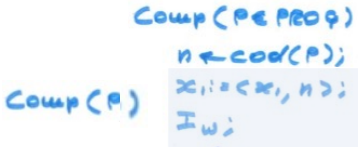
\includegraphics[scale=0.6]{images/compi_Iw.png}
\end{figure}
Prima di tutto calcolo la codifica di $P$, poi la posso cablare nella variabile $x_1$
ed infine chiamo l'interprete (il listato precedente descritto).
\begin{itemize}
    \item \textbf{programmabile}: nel listato di un programma RAM si può calcolare
          tranquillamente la codifica.
    \item \textbf{completo}: in nessuno dei 3 passaggi rischiamo di andare in loop.
    \item \textbf{corretto}: \textit{mantiene la semantica?} Vediamo che la semantica
          del programma compilato non è altro che la semantica dell'interprete chiamata
          sulla coppia, ma questa sappiamo essere l'esecuzione del programma $n$ su $x$, che
          ha sua volta è esattamente l'esecuzione del programma $P$ su $x$:
          $$\Psi_{Comp(P)}(x)=\Psi_{I_W}\left(\langle x,n\rangle\right)=\varphi_n (x)=\varphi_P (x)$$
          $$P\in PROG\rightarrow Comp(P)\in W-PROG$$
          quindi è corretto.
\end{itemize}
Quindi è un compilatore da programma RAM a WHILE funzionante e corretto.
$$F(RAM)\subseteq F(WHILE)$$
La presenza di questo compilatore ci presenta in maniera formale che i \textit{goto}
possono non essere utilizzati nella programmazione strutturata.
\paragraph{Teorema di Böhm Jacopini - 1970}\mbox{}\\
Per ogni programma (RAM) con \textit{goto} ne esiste uno equivalente in linguaggio
strutturato (WHILE).
\begin{itemize}
    \item Significa che la programmazione a basso livello può essere tranquillamente
          sostituita da quello ad alto livello.
    \item Quindi il \textit{goto} va eliminato.
\end{itemize}

\paragraph{Conseguenza 1 $F(RAM)=F(WHILE)$}\mbox{}\\
Sapevamo già che $F(WHILE)\supseteq F(RAM)$ (o viceversa) grazie alla presenza
di un apposito compilatore, ed adesso sappiamo che grazie ad un interprete
(che viene trasformato "\textit{rozzamente}" in un compilatore) $F(WHILE)\subseteq F(RAM)$
Quindi quello che abbiamo ottenuto:

Che la potenza computazionale di una macchina piccola come quella RAM è esattamente
identica a quella di una macchina WHILE molto più complessa , entrambe le macchine sono in
grado di calcolare la stessa cosa.
$$F(RAM)=F(WHILE)$$
Utilizzando una concatenazione logica, sappiamo che
grazie alla Gödelizzazione che la potenza computazionale di una macchina RAM è equinumerosa
al numero di programmi, che a sua volta sono tanti quanti i numeri naturali (che non sono
equinumerosi a tutte le funzioni calcolabili dai naturali ai naturali):
$$\mathbb{N}^{\mathbb{N}}_\bot\nsim\mathbb{N}\sim PROG \sim F(RAM)=F(WHILE)$$

A questo punto la nozione di calcolabilità si capisce che è intrinseca ai problemi,
questo perché ho provato sia a catturarla con la potenza computazionale di RAM che di WHILE,
ma in entrambi i casi ho catturato la stessa cosa ($\mathbb{N}$). \textit{Riesco
    a catturare il concetto di calcolabilità da un punto più astratto?}

\paragraph{Conseguenza 2: interprete universale}\mbox{}\\
Un altra conseguenza importante derivata dal compilatore e dall'interprete, sappiamo
anche che il nostro interprete $I_W$ è un programma WHILE. Se io do in pasto questo
interprete al compilatore di programmi WHILE, quello che ottengo è un programma
RAM $U$.
$$U=Comp(I_W)\in PROG$$
La semantica di tale programma:
$$\varphi_U\left(\langle x,n\rangle\right)=\Psi_{I_W}\left(\langle x,n\rangle\right)=\varphi_n\left( x\right)$$
abbiamo scoperto che in RAM esiste un programma molto particolare che è in
grado di prendere un qualsiasi programma RAM e di simularlo, e non è un caso che
questo programma si chiami \textbf{interprete universale} RAM. Ovvero un programma
scritto in quel linguaggio di programmazione che è in grado di simulare un qualsiasi
altro programma scritto in quel linguaggio di programmazione.

Questo programma $U$ rappresenta tutta la potenza di tutti i programmi RAM, perché
è in grado di simularli tutti.

\paragraph{Riflessione sul concetto di calcolabilità}\mbox{}\\
Sappiamo che esistono delle funzioni calcolabili e non calcolabili, siccome esistono delle funzioni
non calcolabili è naturale cercare di caratterizzare ciò che è calcolabile, questo lo abbiamo
fatto attraverso la macchina RAM e WHILE. Entrambe però catturano la stessa classe di funzioni
calcolabili, \textit{il concetto di calcolabile non è intrinseco ai problemi? quindi
    un concetto matematico non informatico}.
Quindi a prescindere dallo strumento di calcolo, se riuscirò in questo intento
allora risponderò una volta per tutte a questo quesito (non dipenderà mai
dallo strumento di calcolo utilizzato). Ne verremo a conoscenza con il formalismo
introdotto da S. Kleene.

\subsection{Concetto di calcolabilità}
Iniziamo a sospettare che questa idea di calcolabilità sorga dai problemi
(\textit{come caratteristica intrinseca dei problemi}) più che dal
tipo di tecnologia che stiamo utilizzando. Quindi si cerca di astrarre il concetto che
si vuole trattare, ovvero quello di \textbf{calcolabilità}.
Quello che vogliamo fare è definire il concetto in modo matematico e assiomatico, in modo
che ci siano solo riferimenti matematici (e non informatici), in modo che si possa utilizzare
tutti gli strumenti matematici (che possono essere spostati in maniera diretta nel mondo informatico).
Dobbiamo ripassare degli strumenti matematici e fissare un linguaggio comune:

\subsubsection{Strumenti matematici (chiusure di insiemi)}
Dato un insieme $U$, si definisce \textbf{operazione} su $U$ una qualunque
funzione
$$op:U\times\dots\times U\rightarrow U$$
che va da $k$-volte il cartesiano di $U$ ad $U$. Il numero $k$ di operazioni cartesiane
non è altro che il numero di argomenti, detto anche \textbf{arietà}.

\paragraph{Per esempio}\mbox{}\\
L'insieme universo è l'insieme dei numeri naturali, per esempio l'operazione somma è un
esempio di operazione binaria, la somma è una funzione definita su $\mathbb{N}^2$, poiché
prende in ingresso due numeri e ne restituisce uno.
$$+:\mathbb{N}\times\mathbb{N}\rightarrow\mathbb{N}\text{ (operazione binaria)}$$
Anche la radice è un operazione (unaria):
$$\left\lfloor \sqrt{} \right\rfloor:\mathbb{N}\rightarrow\mathbb{N}\text{ (operazione unaria)}$$
Un esempio di operazione $n$-aria è quella del proiettore su di $t$, non
fa altro che restituirà la componente $t$-esima.
$$Pro_t^n:\mathbb{N}\times\dots\times\mathbb{N}\rightarrow\mathbb{N}\text{ (operazione n-aria)}$$

Tornando al nostro discorso, definiamo con \textbf{chiusura} di un insieme $A\subseteq U$
rispetto ad un operazione $op:U^k\rightarrow U$, quando il risultato dell'operazione è ancora
un elemento appartenente all'insieme $A$.
$$\forall a_1,\dots,a_k\in A:op(a_1,\dots,a_k)\in A$$

\paragraph{Esempio}\mbox{}\\
L'insieme dei numeri pari è chiuso rispetto alla somma (2+2=4), la controparte invece no, l'insieme
dei numeri dispari non è chiuso rispetto alla somma (3+3=6).

In generale questo concetto di chiusura può essere esteso ad un insieme di operazioni $\Omega$,
un insieme viene considerato chiuso se è chiuso per ciascuna operazione $\in\Omega$.
\paragraph{Esempio}\mbox{}\\
$$\Omega=\{+,*\}$$
L'insieme dei numeri pari è chiuso rispetto ad $\Omega$ (2*4=8 e 2+4=6). Mentre l'insieme
dei numeri dispari non è chiuso rispetto ad $\Omega$ poiché non è chiuso rispetto alla somma.

Consideriamo il seguente problema, sia $A\subseteq U$ e $op:U^k\rightarrow U$. Quale è il più
piccolo sottoinsieme di $U$ che contiene $A$, che sia chiuso rispetto all'operazione $op$?
(Notare che sono tre condizioni e non due). Voglio allargare $A$ il meno possibile in maniera
che contenga $A$ ma garantisca la chiusura rispetto ad $op$.
\begin{figure}[H]
    \centering
    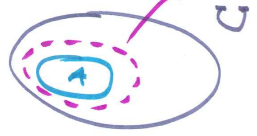
\includegraphics[scale=0.5]{images/insieme_piu_piccolo.png}

\end{figure}

Alcune risposte ovvie:
\begin{itemize}
    \item Se $A$ è chiuso rispetto ad $op$, allora l'insieme cercato è $A$ stesso.
    \item Sicuramente $U$ soddisfa 1 e 2. Però $U$ potrebbe avere il difetto di non
          essere il più piccolo (non è detto che sia il più piccolo).
\end{itemize}
Consideriamo il seguente esempio: sia $A=\{2,3\}\subseteq\mathbb{N}$ come operazione
abbiamo la somma $+:\mathbb{N}^2\rightarrow\mathbb{N}$, banalmente vediamo che $A$ è un insieme
che non può essere chiuso rispetto alla somma. Quale è il più piccolo sottoinsieme di $\mathbb{N}$
che contiene $A$ ed è chiuso rispetto a $+$?
Sappiamo che sicuramente $\mathbb{N}$:
\begin{enumerate}
    \item contiene $A$
    \item è chiuso rispetto a $+$
    \item non è il più piccolo che soddisfa le precedenti due condizioni (1 e 2).
\end{enumerate}
Il problema è dato dal fatto che il risultato dell'operazione da un risultato che sarà
al di fuori di $A$, ma costruendo questo insieme man mano che eseguo
l'operazione e poi aggiungo il nuovo numero al sottoinsieme, allora al termine delle operazioni quello
che avrò sarà il più piccolo sottoinsieme (approccio euristico costruttivo) chiuso rispetto all'operazione.

\paragraph{Teorema}\mbox{}\\
Sia $A\subseteq U$ e $op:U^k\rightarrow U$. Sia Il più piccolo sottoinsieme di $U$
contenente $A$ e chiuso rispetto ad $op$, il quale si ottiene calcolando la \textbf{chiusura di $A$
    rispetto a $op$}, l'insieme $A^{op}$ definito induttivamente come:
\begin{enumerate}
    \item $\forall a\in A\implies a\in A^{op}$
    \item $\forall a_1,\dots,a_k\in A^{op}\rightarrow op(a_1,\dots,a_k)\in A^{op}$
    \item Nient'altro sta in $A^{op}$
\end{enumerate}
La definizione induttiva dice che nella base dell'induzione sono presenti tutti gli elementi
originari in $A^{op}$. Ed ogni elemento a cui si applica l'operazione è un elemento
presente all'interno dell'insieme. Questa definizione è identica alla definizione "più
operativa" di $A^{op}$:
\begin{enumerate}
    \item Metti in $A^{op}$ tutti gli elementi di $A$.
    \item Applica $op$ a una $k$-tupla di elementi in $A^{op}$
    \item Trovi un risultato che non è già in $A^{op}$ allora
          aggiungilo ad $A^{op}$
    \item Ripeti i punti 2 e 3 finché $A^{op}$ cresce.
    \item Output $A^{op}$
\end{enumerate}

\paragraph{Esempi di chiusure}\mbox{}\\
Voglio il più piccolo sottoinsieme di $\mathbb{N}$ contenente $A=\{2,3\}$ e chiuso rispetto
a $+\rightarrow A^+$, come ottenerlo "operativamente"?
\begin{enumerate}
    \item $A^+\leftarrow A$
    \item $(2+3)=5 \notin A^+ \rightarrow A^+ =\{2,3,5\}$
    \item $(2+2),(3+3),(5+5),(2+5),(3+5), \notin A^+\implies A^+=\{2,3,4,5,6,7,8,10\}$
    \item \dots
\end{enumerate}
Ottenendo in output $A^+=\mathbb{N}\setminus\{0,1\}$
Questo è anche dimostrabile banalmente con i risultati di un \textbf{equazione diofantea}
che utilizza gli elementi iniziali dell'insieme di $A$.

Un altro esempio, voglio il più piccolo sottoinsieme di $\mathbb{N}$ contenente $A=\{7,10\}$
e chiuso rispetto a $\dot{-}$ (\textbf{sottrazione troncata}).
$$A^{\dot{-}}=\{0,1,2,\dots,10\}=\mathbb{Z}_{11}$$
Tutti i numeri da 0 a 10 sono in grado di generare un numero all'interno dello stesso
insieme, risultando chiuso rispetto all'operazione di sottrazione troncata.

Un altro esempio, voglio il più piccolo sottoinsieme di $\mathbb{N}$ contenente $A=\{0\}$
che sia chiuso rispetto a $+$.
$$A^+=\{0\}=A$$
L'insieme $A$ è già chiuso rispetto alla somma.

Un'altro esempio, voglio il più piccolo sottoinsieme di $\mathbb{N}$ contenente $A=\{0\}$
e chiuso per $succ(n)=n+1$
$$A^{succ}=\mathbb{N}\text{ se }A=\{1\}\implies A^{succ}=\mathbb{N}^+$$

Lo stesso concetto di chiusura si può estendere rispetto ad un insieme di operazioni, $\Omega=\{op_1,\dots,op_t\}$,
ogni operazione ha una proprietà arietà $k_1,\dots,k_t$ di argomenti. Vogliamo il
più piccolo sottoinsieme di $U$ contenente $A$ tale che sia chiuso rispetto ad $\Omega$. Questo
viene chiamato come \textbf{chiusura di $A$ rispetto ad $\Omega$}, ciò è l'insieme $A^\Omega$
definito induttivamente (induzione strutturale) come:
\begin{itemize}
    \item $\forall a\in A\implies a\in A^\Omega$ (base)
    \item $\forall i\in\{1,\dots,t\}, \forall a_1,\dots,a_{k_i}\in A^\Omega \implies op_i(a_i,\dots,a_{k_i})\in A^\Omega$
    \item Nient'altro è presente in $A^\Omega$
\end{itemize}
Anche qui ovviamente essendo una definizione induttiva di un insieme induttivo se devo dimostrare
una proprietà su $A^\Omega$ la dimostro per induzione strutturale.
Analogamente possiamo dare una definizione più "operativa" (o costruttiva), al caso
dove $|\Omega|=1$, quindi si effettua tutte le operazioni possibili finché non sarà più
possibile estendere l'insieme che si sta costruendo si avrà il più piccolo sottoinsieme di
$U$ che è chiuso rispetto all'insieme di operazioni $\Omega$.

Questi sono esattamente i concetti che ci serviranno per definire in maniera astratta il concetto
di calcolabilità (quindi che astrae da qualunque connotato informatico). Il nostro approccio
sarà così strutturato:
\begin{enumerate}
    \item Partiremo da un nucleo di tre funzioni $ELEM$ che saranno così facili che "qualunque"
          idea di calcolabile si voglia proporre le deve considerare calcolabili. Si vedrà
          subito che quelle tre funzioni non possono essere tutte le funzioni calcolabili, quindi
          sarà obbligatorio ampliare il nucleo di sicura calcolabilità.

    \item Per l'ampliamento del nucleo introdurremo un insieme $\Omega$ di operazioni su funzioni,
          ovvero operazioni che prendono funzioni e restituiscono funzioni (per esempio la
          composizione di funzioni). Usiamo delle funzioni che mi generano altre funzioni, questo
          insieme $\Omega$ è fatto in maniera che sia calcolabile, sono banalmente implementabili in
          qualunque linguaggio di programmazione. Sono operatori che agiscono su cose calcolabili ($ELEM$)
          e sicuramente generano cose calcolabili data la loro semplice implementazione.

    \item Calcolerò la chiusura di $ELEM^\Omega=\mathcal{P}$, il risultato sarà una classe di funzioni
          che sarà la nostra idea di calcolabilità data da un punto di vista puramente matematico, si chiamerà
          \textbf{classe delle funzioni ricorsive parziali}.
\end{enumerate}
(approccio di Kleene).
\begin{figure}[H]
    \centering
    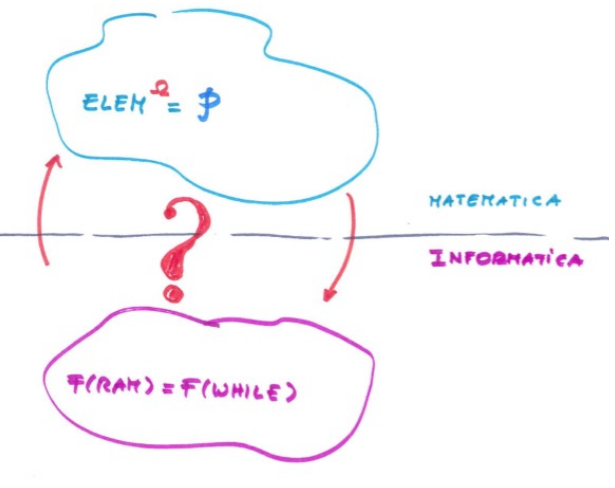
\includegraphics[scale=0.5]{images/mat_info.png}
\end{figure}
Abbiamo due idee di calcolabilità una data dal punto di vista informatico e matematico, la domanda che ci
dovremo porre è \textit{l'approccio matematico è in grado di catturare interamente l'approccio informatico?}
Dobbiamo trovare un punto dove le due idee coincidono, quindi ritrovare ciò che abbiamo definito in maniera informatica
con gli strumenti matematici (che saranno sempre quelli per l'eternità).


\subsubsection{Il nucleo di funzioni calcolabili}
L'insieme delle funzioni elementari (intuitivamente calcolabili) è composto da tre funzioni.
$$ELEM=\{$$
$$\textit{successore: }s(x)=x+1, x\in\mathbb{N},$$
$$\textit{zero: }0^n(x_1,\dots,x_n)=0, x_i\in\mathbb{N},$$
$$\textit{proiettori: }pro_k^n(x_1,\dots,x_n)=x_k,x_i\in\mathbb{N}\}$$

\begin{itemize}
    \item La funzione successore è in grado di effettuare una somma atomica ad una certa quantità.
    \item La funzione zero che restituisce sempre 0.
    \item La funzione proiezione è in grado di restituire un $k$ fissato da una $n$-upla.
\end{itemize}
La nostra idea di calcolabilità si origina da qui poiché sono funzioni
banalmente calcolabili (un programma WHILE è banalmente scrivibile). Questa classe delle funzioni
elementari deve essere un punto da cui partire, poiché sono presenti delle funzioni che
sono estremamente semplici da calcolare ma non presenti nel nucleo iniziale (es., predecessore, una funzione
che sommi 2 anziché 1 \dots).

\textit{Quindi cosa devo fare?} Devo ampliare la classe delle funzioni elementari. Quindi
si pensa di mettere in campo degli operatori che prendono in ingresso delle funzioni e restituiscono
delle funzioni. \textit{Quale é il primo operatore che prende funzioni e restituisce funzioni?}
La \textbf{composizione} di funzione, indicata con $\circ$ prende in ingresso due funzioni e restituisce
la composizione di due funzioni passata come argomento. Quella che vogliamo implementare è una
composizione su più funzioni non solo 2.

\paragraph{L'operatore di composizione di funzioni}\mbox{}\\
Sia $h:\mathbb{N}^k\rightarrow\mathbb{N}$ e $g_1,\dots,g_k:\mathbb{N}^n\rightarrow\mathbb{N}$,
denoteremo $\underline{x}\in\mathbb{N}^n$.
Definisco la composizione degli argomenti come $COMP(h,g_1,\dots,g_k):\mathbb{N}^n\rightarrow\mathbb{N}$
definito come
$$COMP(h,g_1,\dots,g_n)(\underline{x})=h(g_1(\underline{x}),\dots,g_k(\underline{x}))$$
Si parte dalla ennupla $\underline{x}$ la si da in pasto alla prima fino alla $k$-esima funzione,
il risultato di ogni funzione viene dato in pasto alla funzione $h$ per ottenere la composizione.
Notiamo che il caso di una composizione con due funzioni è un caso particolare di questo che è
quello generale.
\begin{figure}[H]
    \centering
    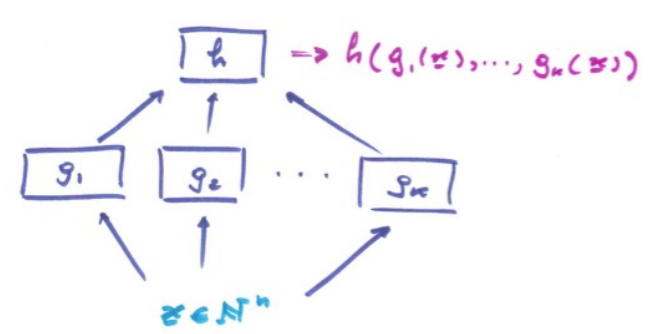
\includegraphics[scale=0.5]{images/composizione_ooperazine.png}
\end{figure}
L'operazione di composizione suona come qualcosa di implementabile, come potrebbe essere
fatto un programma che calcola la composizione di funzioni. La mia idea di calcolabilità
se viene espansa con questo operatore è una cosa corretta, perché parte da cose calcolabili
per generare cose calcolabili.
\paragraph{Ampliamo ELEM chiudendo rispetto a COMP}\mbox{}\\
$ELEM^{COMP}$ effettivamente amplia $ELEM$, infatti:
$$f(x)=x+2\notin ELEM\text{ ma }f(x)\in ELEM^{COMP}$$
Non fosse altro che la mia funzione x+2, è banalmente dimostrabile che $f(x)$ (la funzione
che somma 2 ad x) appartiene ad $ELEM^{COMP}$, questo perchè basta
comporre la funzione successore con se stessa. Infatti $$f(x)=COMP(s,s)(x)=s(s(x))=s(x+1)=x+2=f(x)$$

Abbiamo visto che qualcosa in più riusciamo a calcolare, ma la domanda è \textit{questa
    nuova classe di funzione è considerabile come la nuova classe di tutte le funzioni
    calcolabili oppure manca qualcosa?} Purtroppo questo primo ampliamento non basta a definire
un intera classe di funzioni calcolabili. Per esempio la somma di due numeri non è
calcolabile, ed è facile anche da dimostrare la non appartenenza ad $ELEM^{COMP}$. Devo
ampliare ancora il mio insieme, perché sono presenti ancora funzioni troppo banali che devono
essere considerate calcolabili.

\paragraph{L'operatore di ricorsione primitiva}\mbox{}\\
A tutti è nota la definizione induttiva di fattoriale di $n$, il concetto di questo
operatore matematico è descrivibile induttivamente con la seguente espressione
\[
    fatt(n)=
    \begin{cases}
        1                & n=0 \\
        n\cdot fatt(n-1) & n>0
    \end{cases}
\]
Allora introduciamo l'operatore di ricorsione primitiva $RP$. Per definire tale
operatore necessito di due funzioni argomento $g,h$ (una con una singola ennupla come
argomenti, l'altra con una ennupla più altri due argomenti).
$$g:\mathbb{N}^n\rightarrow\mathbb{N}$$
$$h:\mathbb{N}^{n+2}\rightarrow\mathbb{N}$$
rispettivamente $g(\underline{x})$ e $h(z,y,\underline{x})$ con $\underline{x}\in\mathbb{N}^n$.
L'operatore di ricorsione primitiva prende in ingresso due funzioni e restituisce
una terza funzione ottenuta per \textbf{ricorsione} delle altre due. La ricorsione
primitiva applicata ad $h$ e $g$ restituisce una nuova funzione $f$ che dipende da
una sola ennupla $\underline{x}$ e da un solo parametro $y$ che è definita
\[
    RP(h,g)=f(\underline{x},y)=
    \begin{cases}
        g(\underline{x})                          & y=0 \\
        h(f(\underline{x},y-1),y-1,\underline{x}) & y>0
    \end{cases}
\]
Notiamo che nel caso in cui il parametro $y$ sia 0, la funzione $g(x)$ non è altro che
il caso base, ma ricordiamo che effettivamente $g$ può essere una qualsiasi funzione.
Mentre quando il parametro $y$ è positivo notiamo che la funzione restituita da $RP$ è
la composizione della funzione $h$ su $f$ su valori $y$ minori (\textbf{passo induttivo}).
In particolare si vede che è una \textbf{induzione} che generalizza il concetto di ricorsione.

Questa generalizzazione ci permette di definire funzioni in termini di se stesse, le
definizione ricorsive a cui siamo abituati sono casi particolari di questo caso generale. Sia
risaputo che tutti i metodi per la risoluzione di equazioni differenziali utilizzano
questa forma tabella come risoluzione.

Ora ampliamo ulteriormente $ELEM$
$$ELEM^{COMP,RP}=RICPRIM=\{\text{funzioni ricorsive primitive}\}$$
la chiusura comincia a creare una classe abbastanza consistente di funzioni, che contiene
anche molte funzioni complicate (anche quelle differenziali). Prende il nome come
\textbf{classe delle funzioni ricorsive primitive}. Questa classe contiene la funzione
somma tra due numeri.
\[
    somma(x,y)=
    \begin{cases}
        x=Pro^2_1(x,y)  & y=0 \\
        s(somma(x,y-1)) & y>0
    \end{cases}
\]
questo utilizzando il successore ed il proiettore, ma è anche possibile definire il prodotto
riutilizzando la somma (e via via anche l'esponenziale).
\[
    prodotto(x,y)=
    \begin{cases}
        0=0^2(x,y)                & y=0 \\
        somma(x, prodotto(x,y-1)) & y>0
    \end{cases}
\]
possiamo definire l'operazione di $\dot{-}$ definendo a priori l'operatore di predecessore
\[
    P(x)=
    \begin{cases}
        0   & x=0 \\
        x-1 & x>0
    \end{cases}
    \implies
    x\dot{-}y=
    \begin{cases}
        x                & y=0 \\
        P(x)\dot{-}(y-1) & y>0
    \end{cases}
\]
Si può facilmente notare che la classe delle funzioni ricorsive primitive è una classe
importante che ricopre molte funzioni.

\subsubsection{$RICPRIM$ vs $F(WHILE)$}
$RICPRIM$ contiene molte funzioni e potrei già chiedermi se ho raggiunto $F(WHILE)$. Mostreremo
che $RICPRIM\subseteq F(WHILE)$ per induzione strutturale. Vogliamo capire che tipo di relazione
c'è tra la mia idea di calcolabilità matematica e informatica. Quello che mostreremo
è che questa idea di calcolabilità matematica è inclusa all'interno di quella informatica.

Ovvero che ogni funzione presente in $RICPRIM$ sia $WHILE$-programmabile, ovvero che sia
possibile scrivere un programma $WHILE$ che la calcoli. Significa che siamo sulla strada
giusta che ci stiamo muovendo su qualcosa di significativo.

Possiamo notare che però in $RICPRIM$ sono presenti funzioni totali, ovvero che terminano,
le funzioni non possono andare in loop, quindi l'inclusione dovrà essere per forza propria
se dimostrata.
La dimostrazione seguirà i seguenti punti:
\begin{itemize}
    \item Definizione induttiva di $RICPRIM=ELEM^{COMP,RP}$
          \begin{enumerate}
              \item Le funzioni in $ELEM$ sono in $RICPRIM$
              \item Se prendo delle funzioni $RICPRIM$ allora la loro composizione è
                    $RICPRIM$ anch'essa.
              \item Se prendo delle funzioni $RICPRIM$ allora la loro composizione mendiante l'operatore
                    di ricorsione primitiva genera una funzione $RP$.
              \item Nient'altro è in $RICPRIM$
          \end{enumerate}
\end{itemize}

Quindi data questa definizione induttiva abbiamo dimostrato che $ELEM\subseteq F(WHILE)$,
proseguirò sempre per induzione sui seguenti punti:
\begin{itemize}
    \item Assumo per induzione che $h,g_1,\dots,g_k\in RICPRIM$ siano in $F(WHILE)$
          e dimostro che $COMP(h,g_1,\dots,g_k)\in F(WHILE)$
    \item Assumo per ipotesi induttiva che $g,h\in RICPRIM$ siano in $F(WHILE)$
          e dimostro che $RP(g,h)$ e $F(WHILE)$.
\end{itemize}

allora per induzione avrò dimostrato che le ricorsive primitive sono un sottoinsieme
dell'insieme $WHILE$.

\subsubsection{$RICPRIM\subseteq F(WHILE)$}
\begin{itemize}
    \item passo base: $ELEM\subseteq F(WHILE)$ (sappiamo calcolare funzione successore, zero
          e proiezione k-esima con un programma WHILE).
    \item passi induttivi:
          \begin{itemize}
              \item
                    Consideriamo delle funzioni $h,g_1,\dots,g_k$ per ipotesi induttiva assumo
                    che siano $WHILE$-programmabili ($\in F(WHILE)$). Ovvero che per ciascuna funzione
                    esisti un rispettivo programma $H,G_1,\dots,G_k\in W-PROG$ che le calcola. Ovvero
                    la cui semantica corrisponda esattamente alle funzioni originali.
                    $$\Psi_H=h, \Psi_{G_1}=g_1,\dots,\Psi_{G_k}=g_k$$
                    allora devo mostrarti un programma WHILE che calcoli la loro composizione.
                    $$COMP(h,g_1,\dots,g_k)=h(g_1(\underline{x}),\dots,g_k(\underline{x}))$$
                    \begin{figure}[H]
                        \centering
                        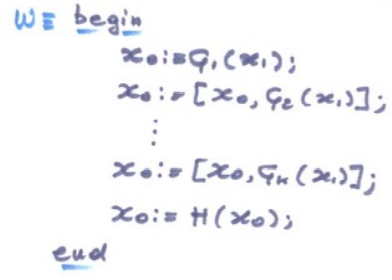
\includegraphics[scale=0.5]{images/while-comp.png}
                        \caption{Programma WHILE che calcola la composizione}
                    \end{figure}
                    Supponiamo che in $x_1$ ci sia il nostro input del programma, in $x_0$
                    calcolo il primo argomento. In realtà $G_1(x_1)$ è una macro del $WHILE$
                    che è in grado di calcolare la sua corrispettiva funzione $g_1$ che
                    so esistere per ipotesi induttiva. Poi in $x_0$ ci condenso il secondo argomento
                    $G_2$ , continuo in questa maniera fino al $k$-esimo argomento. In $x_0$ ottengo la
                    condensazione di tutti gli argomenti su un solo numero, seguendo lo schema di Cantor (
                    non è un problema se abbiamo un numero finito di variabili, i motivi sono già stati spiegati).
          \end{itemize}
          adesso il primo passo induttivo è stato dimostrato, ovvero che la composizione di funzioni
          è WHILE-programmabile.
    \item passo induttivo sull'operatore di ricorsione primitiva: per ipotesi induttiva
          assumo che le due rispettive funzioni $g,h$ siano $WHILE$-programmabili.
          Che quindi esistano $G,H\in W-PROG$ con $\Psi_G=g$ e $\Psi_h=h$.
          Allora riesco a
          a scrivere un programma $WHILE$ che riesce a calcolare l'operazione di ricorsione primitiva.
          \begin{figure}[H]
              \centering
              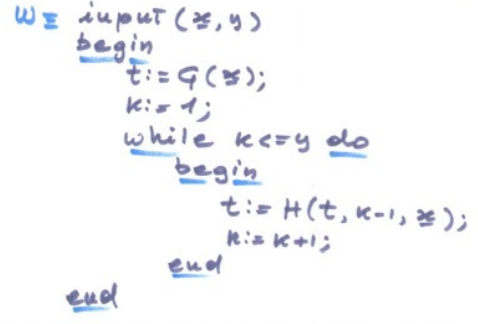
\includegraphics[scale=0.5]{images/while-rico.png}
          \end{figure}
          questo è un programma perfettamente legale che calcola la ricorsione primitiva di due funzioni
          che sono $WHILE$-programmabili.
\end{itemize}
Allora ho dimostrato che per induzione strutturale che la classe delle funzioni ricorsive primitive
è all'interno delle funzioni $WHILE$
$$RICPRIM\subseteq F(WHILE)$$

A sto punto ci chiediamo se questo sotto insieme sia proprio oppure no. Questo però è facile
da dimostrare, tutte le $RICPRIM$ sono funzioni totali:
\begin{itemize}
    \item tutte le funzioni elementari sono totali.
    \item la composizione delle funzioni totali è ancora una funzione totale
\end{itemize}
Chiaramente $F(WHILE)$ contiene anche funzioni \textbf{parziali} (che non terminano),
questo grazie ad i loop che possono non far terminare i programmi.
$$RICPRIM\subsetneq F(WHILE)$$
Significa che devo ampliare ulteriormente $RICPRIM$ per raggiungere $F(WHILE)$

\paragraph{Ulteriori considerazioni su $RICPRIM$}\mbox{}\\
Consideriamo il \textit{while loop} del linguaggio WHILE, notiamo che è possibile riscrivere la stessa cosa
con una sintassi semplificata quella del FOR.
Le $RICPRIM$ caratterizzano la potenza computazionale con un linguaggio più semplice
di quello WHILE, ovvero il $FOR$ language, questo come un \textit{for loop} del PASCAL dove è presente
una variabile di controllo che scandisce le iterazioni, che parte da un certo valore
e termina in un altro valore e che non può essere toccata nel FOR.

Prendiamo tale $FOR$-language, e vediamo che le $RICPRIM$ sono esattamente la classe delle funzioni
calcolate da questo linguaggio che ha un numero di iterazioni che è fissato e non
potrà mai andare all'infinito (non stiamo considerando for loop del C/Java ma quello del PASCAL).
$$RICPRIM=F(FOR)\subsetneq F(WHILE)$$
Questa è una inclusione propria.

\paragraph{Funzioni di Ackermann}\mbox{}\\
Ora effettuiamo un ulteriore considerazione, ipotizziamo di usare un linguaggio WHILE
che non possa andare in loop, quindi mi restringo ad una classe $\tilde{F}(WHILE)$
di funzioni WHILE che non possono andare in loop. \textit{Adesso come sarà il
    confronto tra il $FOR$ language ed il $WHILE$ indebolito?} L'inclusione è propria?

Le $RICPRIM$ sono incluse propriamente nella classe delle funzioni $\tilde{F}(WHILE)$,
questo è dimostrabile sia per diagonalizzazione che utilizzando la funzione di Ackermann.
Una funzione di Ackermann (1928) è una funzione che non è ricorsiva primitiva ma
può essere calcolata da un programma $WHILE$ che termina.

Questa funzione sfrutta una doppia induzione, perché lo schema ricorsivo della funzione
di Ackermann non è lo stesso di quello delle $RICPRIM$.

\[
    \mathcal{A}(m,n)=
    \begin{cases}
        n+1                                 & m=0      \\
        \mathcal{A}(m-1,1)                  & m>0, n=0 \\
        \mathcal{A}(m-1,\mathcal{A}(m,n-1)) & m,n>0
    \end{cases}
\]
$$\mathcal{A}\notin RICPRIM\implies\mathcal{A}\in\tilde{F}(WHILE)$$
Se usiamo solamente la composizione di $RICPRIM$ non siamo in grado di esprimere tale
classe di funzioni. L'idea è che le $RICPRIM$ hanno un determinato tasso di crescita
che è nettamente inferiore rispetto alle funzioni di Ackermann.

N.B.: Già nel 1927 Sudau aveva proposto una funzione con le stesse caratteristiche
di quella di Ackermann\dots
Occorre ampliare $RICPRIM$\dots
\begin{figure}[H]
    \centering
    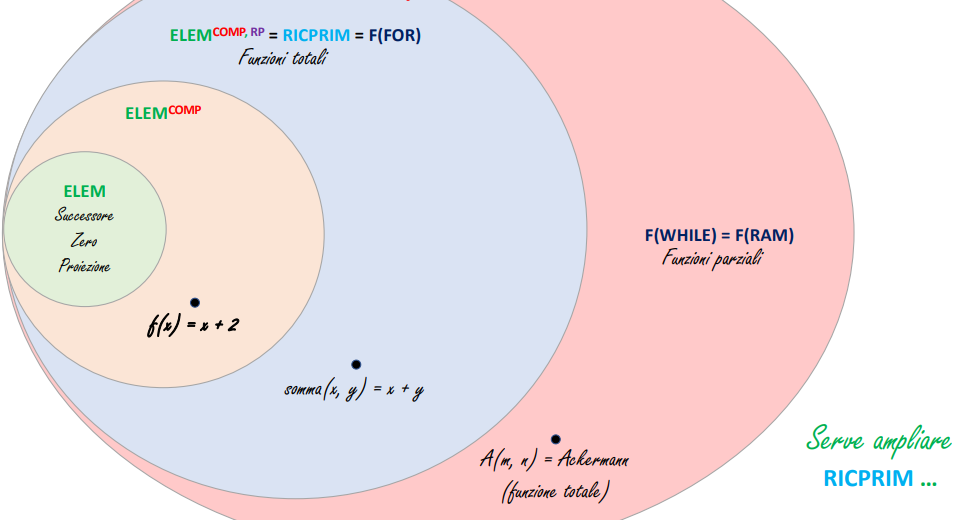
\includegraphics[scale=0.5]{images/classi_funzioni.png}
\end{figure}

\paragraph{Operatore di minimalizzazione di funzioni}\mbox{}\\
Vogliamo ampliare ancora di più l'attuale classe di funzioni, introduciamo il nuovo operatore
di minimalizzazione.
Sia $f:\mathbb{N}^{n+1}\rightarrow\mathbb{N}$, $f(\underline{x},y)$ con
$\underline{x}\in\mathbb{N}^n$. La minimalizzazione di una funzione ad $n+1$ genera una
funzione ad $n$ argomenti, definita come:
\[
    MIN(f(\underline{x},y))=g(\underline{x})=
    \begin{cases}
        y    & \text{se }f(\underline{x},y)=0\text{ e }\forall t<y:f(\underline{x},t)\neq 0 \\
        \bot & \text{altrimenti}
    \end{cases}
\]
$$= \mu y(f(\underline{x},y)=0) (\bot\text{ se }\nexists \text{ tale }y)$$
Nella prima condizione $y$ è tale da essere il più piccolo valore
che azzeri la funzione $f(\underline{x},y)$. Vediamo alcuni esempi di minimalizzazione
di funzioni:
\begin{center}
    \begin{tabular}{c|c}
        \toprule
        $x+y+1$       & $\bot$                 \\
        \midrule
        $x\dot{-}y$   & $x$                    \\
        \midrule
        $y\dot{-}x$   & $0$                    \\
        \midrule
        $x\dot{-}y^2$ & $\lceil\sqrt{x}\rceil$ \\
        \bottomrule
    \end{tabular}
\end{center}

\begin{itemize}
    \item La minimalizzazione di $x+y+1$ è una funzione $g(x)$ che dato un certo $x$ mi deve
          trovare il più piccolo $y$ tale che $x+y+1=0$ (attenzione che è una funzione
          che va da naturali a naturali, quindi i numeri negativi non possiamo considerarli).
          Qualsiasi sia questo numero nella parte sinistra avremo sempre 1, perché con qualunque
          valore di $x$ sia fissato ed $y$ (naturali) non azzererà la funzione.

    \item nel caso della sottrazione troncata il più piccolo $y$ che azzera $x$ è $x$ stesso,
          notare che lo si potrebbe azzerare anche con un $x+1,+2,\dots$ ma questo non sarebbe il più piccolo.

    \item invertendo l'ordine degli operandi il più piccolo $y$ che azzera la funzione è 0.

    \item nell'ultimo caso è la parte superiore della radice di $x$ (la radice quadrata
          è una operazione presente in RICPRIM).

\end{itemize}
Vediamo che con l'operatore di minimalizzazione otteniamo delle funzioni interessanti,
adesso proviamo a chiudere rispetto a queste funzioni.

$$RICPRIM^{MIN}= ELEM^{COMP,RP,MIN}=\mathcal{P}={\text{funzioni ricorsive parziali}}$$
Questa nuova classe di funzioni è detta \textbf{classe delle funzioni ricorsive
    parziali} $\mathcal{P}$. Sicuramente $\mathcal{P}$, che grazie a $MIN$ contiene anche
funzioni parziali, amplia $RICPRIM$ fatto solo da funzioni totali. Ma come si pone
rispetto a $F(WHILE)$?
\subsubsection{$\mathcal{P}\subseteq F(WHILE)$}
Riesco a dimostrare che sia un sottoinsieme (non so se sia tanto quanto $F(WHILE))$,
possiamo dimostrare tenendo conto della natura induttiva delle ricorsive parziali che
sono la chiusura delle ricorsive primitive rispetto all'operatore di minimalizzazione.

\begin{enumerate}
    \item Le funzioni in $RICPRIM$ sono tutte in $\mathcal{P}$
    \item Se $f$ è una $\mathcal{P}$ allora la minimalizzazione di $f$ è
          una ricorsiva parziale.
    \item Nient'altro è in $\mathcal{P}$
\end{enumerate}
Allora cosa faccio per dimostrare che $P\subseteq F(WHILE)$ ? Dimostro che le ricorsive
primitive che sono ricorsive parziali sono $WHILE$-programmabili (ma questo lo abbiamo
già dimostrato precedentemente).

L'unico punto veramente da dimostrare è il passo induttivo, ovvero che il nuovo oggetto
che andiamo a costruire sia $WHILE$-programmabile.

\begin{enumerate}
    \item Dimostrare che le $RICPRIM$ sono $WHILE$-programmabili (fatto).
    \item Sia $f\in\mathcal{P}$ una funzione $WHILE$-programmabile per ipotesi induttiva.
          Allora, esiste un programma $WHILE$ che calcola la minimalizzazione di quella funzione
          $MIN(f)$ (da dimostrare).
\end{enumerate}
\paragraph{Dimostrazione che $MIN(f)$ è $WHILE$-programmabile}\mbox{}\\
Sia $f(\underline{x},y)\in\mathcal{P}$; per ipotesi induttiva, sia $f$ calcolata dal
programma $WHILE$ $F$. Allora devo mostrarti un programma $WHILE$ tale che sia in grado
di calcolare tale funzione:
\[
    MIN(f(\underline{x},y))=g(\underline{x})
    \begin{cases}
        \mu y & f(\underline{x},y)=0             \\
        \bot  & \text{se }\nexists\text{ tale }y
    \end{cases}
\]
questo è un programma che prende in ingresso $x$ e va a cercare il più piccolo $y$
tale per cui la funzione si azzeri.
\begin{figure}[H]
    \centering
    \includegraphics[scale=0.5]{images/while-prog-min.png}
    \caption{Programma WHILE che implementa la minimalizzazione di una funzione}
\end{figure}
Sia tale che questa dicitura è legale, poiché $F$ è un programma $WHILE$, se però
$y$ dovesse mancare questo programma andrà in loop (semantica indeterminata, $\bot$). Si introduce
la possibilità di programmi che vanno in loop.

Per induzione strutturale abbiamo mostrato che $\mathcal{P}\subseteq F(WHILE)$. Sorge una
domanda, \textit{la nostra "idea teorica" di calcolabilità $\mathcal{P}$ raggiungerà
    quella "pratica" di $F(WHILE)$? Può valere $F(WHILE)\subseteq\mathcal{P}$?}

Nel caso in cui si possa dimostrare tale inclusione (e quindi poi dimostrare che $F(WHILE)=\mathcal{P}$).

\subsubsection{Dimostrazione $F(WHILE)\subseteq\mathcal{P}$}
Vogliamo dimostrare
$$F(WHILE)=\{\Psi_w : w\in W-PROG\}\subseteq\mathcal{P}=ELEM^{COMP,RP,MIN}$$
le funzioni $WHILE$ programmabili sono anche delle ricorsive parziali.
$$\Psi_w\in F(WHILE)\implies\Psi_w\in\mathcal{P}=ELEM^{COMP,RP,MIN}$$
Quindi prendiamo una funzione tale e dimostriamo che essa sia ricorsiva parziale, ma questo
per definizione vuol dire dimostrare che $\Psi_w$ può essere ottenuta come composizione,
ricorsione primitiva e minimalizzazione a partire da funzioni in $ELEM$.

Se riesco a dimostrare questo allora ho dimostrato che la semantica di un qualsiasi programma
$WHILE$ è ricorsiva parziale.

Ricordiamo come è definita la semantica di un programma $WHILE$ si definisce a partire
dall'input $x$ inserito in una funzione che inizializza la macchina (delle 21 variabili
disponibili $x_1=x$ ed il resto impostate a 0). Dopo di che si fa agire la semantica nel
programma $w$, la quale è la funzione stato prossimo, ci restituisce lo stato successivo.
L'output è lo stato finale che viene salvato sul registro/variabile 0 delle 21 disponibili,
questo significa effettuare la proiezione.
$$\Psi_w(x)=Pro_0^{21}([w](W-in(x)))$$
(la funzione stato prossimo $[C](\underline{x})=\underline{y}$ calcola lo stato
$\underline{y}\in\mathbb{N}^{21}$ a seguito dall'esecuzione del comando $WHILE$ $C$
partendo dallo stato $\underline{x}\in\mathbb{N}^{21}$). In pratica la semantica
WHILE mi preleva l'output (proiezione) dopo l'esecuzione del programma $w$ (funzione
stato prossimo) inizializzato (funzione di inizializzazione).

Quindi vogliamo dimostrare che $\Psi_w(x)=Pro_0^{21}([w](W-in(x)))$ faccia parte delle
ricorsive parziali, noto che la semantica di un programma $WHILE$ si ottiene effettuando
la composizione di una funzione elementare (la proiezione) con la funzione stato prossimo.
Allora questo significa che posso rappresentare con le ricorsive parziali la funzione
stato prossimo, vediamo perché:
\begin{enumerate}
    \item $Pro_0^{21}\in ELEM\implies Pro_0^{21}\in\mathcal{P}$
    \item $\mathcal{P}$ è chiuso rispetto alla composizione
    \item Questo dimostra che $[C](\underline{x})=y\in\mathcal{P}$ allora $\Psi_w\in\mathcal{P}$. Qui
          però c'è da aggiungere un dettagli tecnico, la funzione stato prossimo è definita come $[]():\mathbb{N}^{21}\rightarrow\mathbb{N}^{21}$
          ha come codominio $\mathbb{N}^{21}$ (funzione che va da stati in stati). Mentre $\mathcal{P}$ per come le abbiamo
          definite hanno come codominio $\mathbb{N}$. \textit{Questo è un problema?} a dire il vero no, sappiamo che possiamo
          esprimere ciò con una codifica di 21 elementi utilizzando la lista di Cantor.
\end{enumerate}
Quindi quello che faremo non sarà dimostrare che una funzione da vettore a vettore appartiene
alle funzioni ricorsive ($[C](\underline{x})=\underline{y}\in\mathcal{P}$ con $\underline{x},\underline{y}\in\mathbb{N}^{21}$).
Quanto $f_C(x)=y\in\mathcal{P}$ con $x=[\underline{x}]$ e $y=[\underline{y}]$, ovvero la funzione
correlata con gli stati che non sono visti come vettori ma la codifica di array di 21 elementi (ovvero
gli stati contenuti nelle 21 variabili) secondo Cantor.
\begin{figure}[H]
    \centering
    \includegraphics[scale=0.5]{images/ric-parz.png}
\end{figure}
Quindi diciamo che se dimostro che $f_C$ è ricorsiva parziale allora anche $[C]$ è ricorsiva
parziale. Utilizzando le parentesi quadre per impacchettare gli stati e le proiezioni per
spacchettarli (importante sottolineare che queste operazioni sono sicuramente
funzioni elementari $\in ELEM$).

\paragraph{Dimostrazione che $f_C\in\mathcal{P}$}\mbox{}\\
Dimostrazione per induzione sul comando $C$ che $f_C$ è ricorsiva parziale, quindi prima di
tutto vado ad individuare $f_C$ sulla base del linguaggio $WHILE$ ovvero gli assegnamenti.
\begin{itemize}
    \item $C\equiv x_k :=0$ (azzeramento della componente $k$)
          $$f_{x_k:=0}(x)=[Pro(0,x),\dots,0,\dots,Pro(20,x)]$$
          tutte le operazioni qui effettuate sono ricorsive parziali, le funzioni di proiezione
          sono elementari, fondere con le parentesi quadra consiste in una serie di somme. Quindi
          lo stato prossimo di un azzeramento è una funzione che globalmente è ricorsiva parziale.

    \item $C\equiv x_k:=x_j +/\dot{-}1$ (incremento/decremento di 1)
          $$f_{x_k:=x_j +/\dot{-}1}=[Pro(0,x),\dots,Pro(j,x)+/\dot{-}1,\dots,Pro(20,x)]$$
          anche qui molto similmente,
          prendiamo lo stato $x$ e lo spacchettiamo, raggiungiamo la componente $k$-esima e gli
          sommiamo o decrementiamo di 1 il valore. Il risultato è un numero che è la "condensa"
          dello stato prossimo (identico a prima solo che incremento). Anche qui sono coinvolte
          solo funzioni ricorsive parziali, quindi lo stato prossimo per l'operatore di incremento
          decremento è una funzione ricorsiva parziale.
          $$f_{x_k:=x_j +/\dot{-}1}(x)\in\mathcal{P}$$
\end{itemize}

adesso vediamo la funzione stato prossimo per i comandi composti
\begin{itemize}
    \item $C\equiv \underline{begin}\;C_1;\dots;C_m\;\underline{end}$
          ipotizzando induttivamente che $f_C\in\mathcal{P}$ (la funzione composta)
          $f_C(x)=f_{C_m}(\dots\;f_{C_1}(x)\dots)$
          effettuo la composizione, ovvero applico la funzione diverse volte sulla funzione degli
          altri comandi composti. Però noi sappiamo che la funzione composizione è una funzione
          ricorsiva parziale (questo per ipotesi induttiva).

    \item $C'\equiv\text{while }\;x_k\neq 0\text{ do }C$, consideriamo sempre per ipotesi
          induttiva che la funzione composta faccia parte delle ricorsive parziali $f_c\in\mathcal{P}$

          $$f_{c'}(x)=f_c^{e(x)}(x)\text{ con }e(x)=\mu y(Pro(k,f_c^y(x))=0)$$
          ovvero applichiamo il comando $C$ nello stato $x$ un numero $e$ di volte, tale per cui
          questo numero sia il più piccolo numero di volte che serve per azzerare la variabile $k$.

          Inizio a notare qualcosa che m i piace, ci sono operazioni di minimizzazione e proiezione,
          questi sono costrutti ricorsivi parziali.

          Siamo attualmente tentati da dire che la semantica del $WHILE$ sia ricorsiva parziale, ma
          c'é qualcosa che non va. Ma questa composizione non è un costrutto ricorsivo parziale, questo
          perché questa composizione è parametrizzata rispetto ad $y$. Il nostro operatore $COMP$ è definito
          su un numero costante di argomenti, qui abbiamo un numero di argomenti \textbf{variabili}.
\end{itemize}

Quindi dato che $f_C^{e(x)}$ è la composizione di $f_C$ per $e(x)$ volte, che non è un numero
costante. Io so scrivere $COMP(h,g_1,\dots,g_k)$ con $k$ costante. Quindi ci si chiede
\textit{come rappresentare in $\mathcal{P}$ la composizione di una funzione con se stessa
    un numero \textbf{non costante} di volte?} ovvero l'operatore $T(x,y)=f_C^y(x)$

\[
    T(x,y)=
    \begin{cases}
        x             & y=0 \\
        f_C(T(x,y-1)) & y>0
    \end{cases}
\]
Da notare che questo costrutto è ricorsivo parziale, perchè è ottenuto attraverso una
ricorsione primitiva sfruttando delle funzioni $f_C$ che sappiamo per induzione essere ricorsive
parziali. Ed è proprio quello che ci serviva, posso riscrivere utilizzando l'operatore
ricorsivo parziale:
$$e(x)=\mu y(Pro(x,T(x,y))=0)$$
Questa è la minimizzazione dell'esponente della composizione di funzione, per esprimere
la forma completa mi bastare dire:
$$f_{C'}(x)=f_C^{e(x)}=T(x,e(x))$$
anche lo stato prossimo del comando while è esprimibile con costrutti ricorsivi parziali, quindi
abbiamo dimostrato che $F(WHILE)\subseteq\mathcal{P}$

Allora, abbiamo dimostrato che
$$F(WHILE)=\mathcal{P}$$
\begin{figure}[H]
    \centering
    \includegraphics[scale=0.4]{images/situazione_funz.png}
\end{figure}
Abbiamo caratterizzato matematicamente ciò che prima avevamo definito con un linguaggio
ed una macchina. Da un punto di vista teorico i linguaggi $F(WHILE)$ e $F(RAM)$ si chiamano
\textbf{classe delle funzioni ricorsive parziali}.

Esiste un interessante sottoclasse delle funzioni ricorsive parziali, la \textbf{classe
    delle funzioni ricorsive totali} indicata con $\mathcal{T}$.

\subsubsection{Tesi di Church-Turing}
\begin{figure}[H]
    \centering
    \includegraphics[scale=0.5]{images/church-turing.png}
\end{figure}
Qualunque modello di calcolo sintetizzato negli anni '30 che individuasse le cose
calcolabili va sempre ad attingere dalla classe delle funzioni ricorsive parziali:
WHILE, RAM, Macchine di Turing, $\lambda$-calcolo, Grammatiche, \dots

Tutti questi punti di vista diversi della calcolabilità hanno sempre detto che la classe delle
funzioni calcolabili è sempre quella delle ricorsive parziali $\mathcal{P}$. Per questo
è stata proposta la tesi di Church-Turing (entrambi hanno pensato la stessa cosa): la classe
delle funzioni intuitivamente calcolabili coincide con la
classe delle funzioni ricorsive parziali.

Tutto ciò che pensi sia calcolabile sarà sempre catturato dalla classe delle funzioni ricorsive parziali.
\textit{Perché non si parla di teorema?} Perché non è presente una caratterizzazione di tutti
i modelli di calcolo presenti, la vediamo come una presa di posizione prudente. Fin'ora è
una tesi che è stata sempre confermata da un qualsiasi modello di calcolo ragionevole.

In altre parole, aderendo alla tesi di Church un sinonimo di "calcolabile" è \textit{"ricorsivo parziale"},
mentre se dico che un compito è \textit{"ricorsivo totale"} intendo che è calcolabile da programmi che
non possono andare mai in loop (ovvero che si arrestano su ogni input).

\subsection{Sistemi di programmazione}
In un sistema di calcolo posso studiare altre proprietà, come studiare certi programmi specifici
per un determinato compito. Oppure vorrei poter dimostrare che per certi compiti specifici non
sono in grado di scrivere dei programmi.

Vorrei guardare all'interno di un sistema formale di programmazione e studiare altre proprietà che
non siano la potenza di calcolo. Il nostro atteggiamento sarà quello che abbiamo tenuto fin'ora,
\textit{vogliamo dare delle risposte che siano generali ed astratte, e che non prendano in
    considerazione un solo sistema di programmazione ma tutti i sistemi di programmazione}.

\paragraph{Definizione di sistema di programmazione accettabile}\mbox{}\\
% riprendere appunti
Individuare alcune proprietà (dette assiomi) che auspicabili per un sistema di programmazione
qualunque. Un sistema di programmazione viene definito come \textbf{accettabile} se soddisfa
queste tre proprietà (le quali vengono soddisfatte dal maggior numero di sistemi di programmazione).

Cercherò di dimostrare queste tre proprietà utilizzando questo sistema molto ristretto di assiomi
per dimostrare certi risultati, questi risultati si estendono a tutti i sistemi di programmazione che
soddisfano questo sistema di assiomi.

Definizione di un gruppo utilizzando una serie di proprietà,
per esempio l'insieme $\mathbb{R}$ rispetto alla somma forma un gruppo, ovvero tutti gli insiemi che
soddisfano una serie di assiomi.
Una volta stabilito che cosa è un gruppo si provano i risultati sui gruppi, utilizzando gli assiomi
che definiscono che cosa è un gruppo.

\subsubsection{Proprietà auspicabili per un sistema di programmazione}
Un sistema di programmazione che solitamente definisco dicendo come è fatta la macchina, il linguaggio, \dots
Ma noi vogliamo definire in generale, quindi definiamo un sistema di programmazione utilizzando la sua potenza
computazionale $\{\varphi_i\}_{I\in\mathbb{N}}$

$$\{\varphi_i\}_{i\in\mathbb{N}}=\text{Insieme delle funzioni calcolabili con quel sistema}$$
Dove $i\in\mathbb{N}$ sono le codifiche dei programmi di quel sistema.
Possiamo cercare di ispirarci ad un sistema di programmazione particolare, per capire
quali siano le proprietà più auspicabili, consideriamo il sistema RAM:
\begin{enumerate}
    \item \textbf{Potenza computazionale}, ovvero $\{\varphi_i\}=\mathcal{P}$, significa che RAM
          aderisce alla tesi di Church-Turing. Questa mi sembra una proprietà ragionevole da avere,
          questo perché la tesi stessa dice che "ciò che è ragionevolmente calcolabile è la classe della
          funzioni ricorsive parziali", visto che vogliamo un sistema ragionevole vogliamo aderire con
          questa classe di funzioni (non vogliamo nulla di più o di meno).
    \item \textbf{Interprete universale}, ovvero un programma $u\in\mathbb{N}$ tale che
          $\forall x,n\in\mathbb{N}:\varphi(\langle x,n\rangle)=\varphi_n(x)$, ovvero in grado di
          simulare un qualsiasi altro programma scritto in RAM (esso stesso è scritto in RAM). Possiamo
          rivedere i passi con cui abbiamo dimostrato l'esistenza di questo programma universale:
          La presenza di un interprete universale è molto interessante, vogliamo trattare sistemi di programmazione
          dove è presente un interprete universale, questo perché ci garantisce un algebra dei programmi, ovvero
          la possibilità di trasformare un programma in un altro programma.
    \item \textbf{Teorema $S_1^1$}: è possibile scrivere dei programmi che automaticamente danno in output dei programmi
          più specifici a partire da un programma più generale. Il programma più specifico è un programma generale dove
          alcuni input vengono prefissati. Il teorema garantisce che per quel sistema sono in grado di scrivere un programma
          che preso in ingresso un programma generale ed un modo di fissare un suo input riesco ad ottenere un listato dove uno dei
          suoi input è stato fissato (quindi una versione più specifica).
          Per esempio, in un sistema di programmazione $RAM$ consideriamo $P\in PROG:\varphi_P(\langle x,y\rangle)=x+y$.
          \begin{figure}[H]
              \centering
              \includegraphics[scale=0.5]{images/programma_p.png}
              \caption{Codice del programma $P$}
          \end{figure}

          Prima di tutto prende un addendo estraendo il primo numero da sommare e lo mette in $R_2$,
          nel registro $R_3$ estrapola l'altro addendo (le macro sono tutte ricorsive parziali). \textit{Siamo
              in grado di scrivere un programma che dia in output il listato di un programma $\overline{P}$
              la cui semantica sia $x+3$?}
          \begin{figure}[H]
              \centering
              \includegraphics[scale=0.5]{images/programma_pseg.png}
              \caption{Codice del programma $\overline{P}$}
          \end{figure}
          Questa è una versione più specifica, perché uno dei due input è
          fissato. Questo è possibile caricando in $R_0$ mi preparo il numero 3, una volta che ho questa costante
          mi preparo in $R_1$ mi preparo la coppia $\langle x,3\rangle$ poi ripulisco $R_0$, alla fine avvio $P$.
          Quando avvio $P$, esso prenderà l'input da $R_1$ che ha come secondo elemento della coppia una costante 3,
          e salverà l'output su $R_0$. Questo programma lo chiamerò $S_1^1$, questo modo di calcolare
          programmi specifici a partire da un programma generale, supponiamo di avere un programma $n$
          in $RAM$ che parte da due input e un $\overline{n}$ che ne ha bisogno solo di 1 perché l'altro
          è fissato.

          \begin{figure}[H]
              \centering
              \includegraphics[scale=0.5]{images/psegnato.png}
          \end{figure}

          $$S_1^1(n,y)=\overline{n}\text{ tale che }\varphi_{\overline{n}}(x)=\varphi_n(x,y)$$
          Si chiama $S^1_1$ perché funziona su programmi $n$ che hanno 2 input, e fissa 1 input (il
          pedice) e lascia libero l'altro input (l'apice).

          Posso esplicitare la funzione $S_1^1$ come
          $$S_1^1(n,y)=\overline{n}=\langle 0,\dots,0,s,t,n\rangle$$
          dove:
          \begin{itemize}
              \item codifica delle prima $y$ istruzioni che hanno come aritmetizzazione tutte 0.
              \item $s$ è la codifica della coppia.
              \item $t$ è la codifica dell'azzeramento di $R_0$.
              \item $n$ è la codifica del mio programma $P$.
          \end{itemize}
          Che caratteristiche ha questa funzione? Prima di tutto è una funzione \textbf{totale}, inoltre
          è una funzione \textbf{programmabile}. Questo significa che la funzione $S_1^1\in\mathcal{T}$,
          è una funzione \textbf{ricorsiva totale} (non andrà mai in loop). In sintesi
          abbiamo scoperto che nel sistema di programmazione RAM, esiste una funzione ricorsiva totale che
          accetta i seguenti argomenti: un codice $n$ di un programma con due input, un valore $y$ su cui
          fissare uno dei due input. Questa funzione produce un numero $S_1^1(n,y)$ che è il codice del
          programma che esattamente lo stesso significato di $n$ dove $y$ è fissato su una delle variabili.
          Significa che per il sistema $RAM$ vale il teorema $S_1^1$: Dato il sistema $RAM$ $\{\varphi_i\}$,
          esiste una funzione $S_1^1\in\mathcal{T}$ tale che $\forall n,x,y\in\mathbb{N}$:
          $$\varphi_n\left(\langle x,n\rangle\right)=\varphi_{S_1^1(n,y)}(x)$$
          Anche il teorema $S_1^1$ è una proprietà auspicabile, per le stesse ragioni per cui mi piacerebbe
          un interprete universale, perché sono in grado di avere un algebra dei programmi che mi permetta di
          prendere un programma e restringerlo sul dominio degli input.

          Il teorema $S_n^m$ è la generalizzazione del teorema $S_1^1$, abbiamo un programma composto da
          $m+n$ variabili, dove si fissano gli ultimi $n$ input e si lasciano variare i primi $m$.
          Formalmente, dato $\{\varphi_i\}$ RAM, esiste una funzione $S_n^m\in\mathcal{T}$ tale che per
          ogni programma $k\in\mathbb{N},\underline{x}\in\mathbb{N}^m$ e ogni $\underline{y}\in\mathbb{N}^n$ vale:
          $$\varphi_k\left(\langle\underline{x},\underline{y}\rangle\right)=\varphi_{S_n^m(k,\underline{y})}\left(\langle\underline{x}\rangle\right)$$
          La dimostrazione è una semplice generalizzazione di quella fornita per il teorema $S_1^1$.
\end{enumerate}

Queste sono le tre proprietà auspicabili di un sistema di programmazione per prenderlo da un punto
di vista teorico. Questi vengono chiamati tre assiomi di Rogers (1959), un sistema di programmazione viene
definito accettabile se:
\begin{enumerate}
    \item aderisce alla testi di Church-turing.$$\{\varphi_i\}=\mathcal{P}$$
    \item esiste un interprete universale.$$\exists u\in\mathbb{N}:\varphi_u\left(\langle x,n\right)=\varphi_n(x)$$
    \item se vale il teorema $S_n^m$.$$\exists S_n^m\in\mathcal{T}:\forall k\in\mathbb{N},\underline{x}\in\mathbb{N}^m,\underline{y}\in\mathbb{N}^n\text{ vale }\varphi_n\left(\langle\underline{x},\underline{y}\rangle\right)=\varphi_{S_n^m(k,\underline{y})(\langle\underline{x}\rangle)}$$
\end{enumerate}
Questi non sono assiomi restrittivi, il rischio è che la serie di assiomi individuano pochi oggetti
perché sono molto restrittivi, in realtà tutti i linguaggi di programmazione che abbiamo
conoscenza soddisfano questi tre assiomi di calcolo.

\subsubsection{Esistenza di compilatori tra S.P.A.}
Dati due linguaggi, una cosa interessante da verificare è: \textit{sono in grado di scrivere
    un compilatore tra questi due linguaggi?} (qualunque essi siano, purché siano sistemi di programmazione
accettabili). Dal punto di vista pratico dipende dai linguaggi che vengono forniti, quello che possiamo
dimostrare però è che qualunque sia la coppia dei linguaggi scelti è che \textbf{sicuramente
    esiste un compilatore tra di essi}.
Dati due sistemi di programmazione accettabili $\{\varphi_i\}$ e $\{\Psi_i\}$ un compilatore è un modo
per trasformare un programma in un altro in maniera che mantenga la semantica. Per noi i
programmi sono numeri, quindi un compilatore è una funzione $t:\mathbb{N}\rightarrow\mathbb{N}$
tale che abbia le seguenti caratteristiche:
\begin{enumerate}
    \item \textbf{Correttezza}: deve valere la semantica, ciò che fa il programma sorgente
          lo deve fare anche il programma oggetto. $\forall i\in\mathbb{N}\text{ vale }\varphi_i=\Psi_{t(i)}$
    \item \textbf{Completezza}: compila ogni $i\in\mathbb{N}$.
    \item \textbf{Programmabile}: esiste un programma che implementa $t$.
\end{enumerate}
Da un punto di vista formale, un compilatore è una funzione che va dai naturali ai naturali che
è ricorsiva totale (punto 2 e 3) e corretta. Quello che si vuole dimostrare è che dati due sistemi di programmazione accettabili
esisterà sempre un compilatore tra essi.
\paragraph{Teorema}\mbox{}\\
Sia $\{\varphi_i\}$ che $\{\Psi_i\}$ valgono gli assiomi degli s.p.a.:
\begin{enumerate}
    \item $\{\varphi_i\}=\mathcal{P}$
    \item $\exists u:\varphi_u\left(\langle x,n\rangle\right)=\varphi_n(x)$
    \item $\exists S_1^1\in\mathcal{T}:\varphi_n\left(\langle x,y\rangle\right)=\varphi_{S_1^1(n,y)}(x)$
\end{enumerate}
devo dimostrare che posso esibire una funzione $t\in\mathcal{T}$ compilatore
che sia ricorsiva totale e che sia corretta (solamente utilizzando questi tre assiomi).
\begin{itemize}
    \item Prendiamo un programma $i$-esimo, $\varphi_i(x)$ in questo sistema di programmazione
          accettabile ho garantiti i tre assiomi. Se uso l'esistenza di un interprete universale allora
          posso dire che esiste un programma $u$ per cui posso simulare il programma
          $$\varphi_i(x)=\varphi_u\left(\langle x,i\rangle\right)$$
    \item Noto che tutto ciò che è calcolato nel sistema $\{\varphi_i\}$, questo grazie
          alla tesi di Church-Turing, e lo stesso vale per $\{\Psi_i\}$. Allora esiste un programma $e$
          in grado di calcolare il programma $u$, ovvero che ha la sua stessa semantica.
          $$\varphi_i(x)=\varphi_u\left(\langle x,i\rangle\right)=\Psi_e\left(\langle x,i\rangle\right)$$
    \item Il terzo assioma mi dice che è possibile rubare una delle variabili in input grazie al
          teorema $S_1^1$.
          $$\varphi_i(x)\overset{(2)}{=}\varphi_u\left(\langle x,i\rangle\right)\overset{(1)}{=}\Psi_e\left(\langle x,i\rangle\right)\overset{(3)}{=}\Psi_{S_1^1(e,i)}(x)$$
\end{itemize}
Il compilatore cercato è la funzione $t(i)=S_1^1(e,i)$ per ogni $i\in\mathbb{N}$, quindi
questa funzione $t(i)$ è effettivamente un compilatore tra i due sistemi di programmazione
accettabili
\begin{enumerate}
    \item $t\in\mathcal{T}$ in quanto $S_1^1\in\mathcal{T}$
    \item $t$ è corretta: $\varphi_i=\Psi_{t(i)}$ per quanto dimostrato in
          $\varphi_i(x)=\varphi_u\left(\langle x,i\rangle\right)=\Psi_e\left(\langle x,i\rangle\right)=\Psi_{S_1^1(e,i)}(x)$
\end{enumerate}
Solamente grazie a queste tre proprietà matematiche sono riuscito a dimostrare che esiste un compilatore
fra due s.p.a.
\paragraph{Corollario}\mbox{}\\
Dati i seguenti s.p.a. $A$,$B$ e $C$, voglio costruire un compilatore tra $A$ e $B$ scritto
nel linguaggio $C$ (sappiamo che esiste tra $A$ e $B$, ma lo vogliamo scrivere nel $C$).\\Dimostrazione:

\begin{itemize}
    \item Per il teorema precedente, esiste il compilatore $t\in\mathcal{T}$ da $A$ a $B$.
    \item Poiché $C$ è un s.p.a., per l'assioma 1, $C$ contiene programmi per tutte le funzioni
          ricorsive parziali.
    \item Dunque, conterrà un programma anche per $t$ che è una funzione ricorsiva totale.
\end{itemize}
In pratica, dimostro che posso scrivere questo compilatore nel con un qualsiasi linguaggio
a patto che sia un s.p.a., non mi interessa il compilatore tra cosa sarà e cos'altro sarà,
quello che sappiamo è che sicuramente esiste.

\subsubsection{Teorema di isomorfismo di Rogers}
In realtà esiste un risultato più forte tra l'esistenza di due compilatori,
esiste un compilatore con una qualità in più tra due sistemi accettabili. Il teorema dice che
dati due s.p.a. $\{\varphi_i\}$ e $\{\Psi_i\}$ esiste sicuramente una funzione $t:\mathbb{N}\rightarrow\mathbb{N}$ tale che:
\begin{enumerate}
    \item $t\in\mathcal{T}$
    \item $\forall i\in\mathbb{N}:\varphi_i=\Psi_{t(i)}$
    \item $t$ è invertibile: $t^{-1}$, significa che è un \textbf{decompilatore}, ovvero un modo
          che sia possibile recuperare il sorgente da cui sono partito con corrispondenza 1:1, ovvero
          una funzione biettiva (che si dice anche isomorfismo).
\end{enumerate}

\subsubsection{Teorema di ricorsione}
\paragraph{Primo quesito}\mbox{}\\
Dato un s.p.a., \textit{esistono all'interno di esso è possibili che al suo interno dei programmi
    che stampano se stessi?} Questi programmi auto replicanti sono detti \textbf{Quine}, questo in onore
di un filosofo americano W.Quine che aveva studiato nell'ambito della logica delle formule che
parlavano di se stesse.
\begin{figure}[H]
    \centering
    \includegraphics[scale=0.5]{images/python.png}
    \caption{Programma Quine in Python}
\end{figure}
Nel caso di linguaggi di programmazione come C, C++,Java, Python, SQL, PHP, \dots
Il fatto che ci siano così tanti casi positivi per così molti linguaggi ci da una sensazione
che la risposta generalmente sia si, ma noi vogliamo una dimostrazione astratta, generale e
formale di ciò.

Per fissare un contesto più matematico possiamo per esempio ambientare questa domanda nel
sistema di programmazione RAM dove sappiamo che tutti i programmi possono essere rappresentati
da dei numeri, allora posso rappresentare il quesito con questa domanda:
$$\exists j\in\mathbb{N}:\varphi_j(x)=j\text{ per ogni input }x\in\mathbb{N}?$$
ovvero dove l'output è il suo listato.

\paragraph{Secondo quesito}\mbox{}\\
Dati due s.p.a., so che è presente un compilatore tra essi, \textit{sono in grado di scrivere
    compilatori completamente errati?} Un compilatore è una trasformazione tra programmi che sono
visti come numeri:
\begin{enumerate}
    \item in grado di compilare un qualsiasi programma automaticamente, questo rappresentato
          dalla funzione $t\in\mathcal{T}$.
    \item la semantica del sorgente deve essere uguale alla semantica dell'oggetto
          $$\forall i\in\mathbb{N}:\varphi_i=\Psi_{t(i)}$$
\end{enumerate}
Un compilatore che è completamente errato è una funzione $t:\mathbb{N}\rightarrow\mathbb{N}$ t.c.
\begin{enumerate}
    \item $t\in\mathcal{T}$
    \item in questo caso il mio compilatore sbaglia sempre la semantica
          $$\forall i\in\mathbb{N}:\varphi_i\neq\Psi_{t(i)}$$
\end{enumerate}
Partendo dall'assunzione che non è possibile carpire la semantica di un programma in ingresso.
Per rispondere a questo quesito dobbiamo introdurre un teorema detto "Teorema di ricorsione".

\paragraph{Teorema di ricorsione}\mbox{}\\
Una risposta precisa ai due precedenti quesiti è data dal \textit{teorema di ricorsione} (Kleene).
Dato una s.p.a. $\{\varphi_i\}$, prendiamo una qualsiasi funzione ricorsiva totale $t:\mathbb{N}\rightarrow\mathbb{N}$,
 definita da programma a programma, allora vale che:
$$\exists n\in\mathbb{N}:\varphi_n=\varphi_{t(n)}$$
ovvero, esisterà un programma la cui semantica non subirà alcuna trasformazione applicata dalla funzione
$t$. Prendiamo $t$ (la funzione trasformazione dei programmi), qualsiasi sia la trasformazione esisterà
almeno un programma che non sarà intaccato da questa trasformazione (qualsiasi trasformazione essa sia).

Grazie al teorema di ricorsione riusciamo a rispondere ai precedenti due requisiti (vedremo
dopo la dimostrazione):
\begin{itemize}
    \item Nel 1° quesito: \textit{esistono Quine negli s.p.a.?} Consideriamo il seguente
          programma $P$
          \begin{figure}[H]
              \centering
              \includegraphics[scale=0.5]{images/P_teoremaric.png}
          \end{figure}
          Notiamo che è un programma che se ne frega, \textit{quale è la semantica di questo
              programma?} (in $RAM$: $\exists j\in\mathbb{N}:\varphi_j(x)=j?$) Notiamo che il programma mette $j$ nel registro, quindi è $j$.
          In poche parole la codifica di questo programma è la lista di Cantor $\langle0,0,\dots, 0\rangle$
          ovvero una funzione $Z(j)\in\mathcal{T}$ che mette $j$ volte lo 0 in lista di Cantor. Ovviamente
          questa è una funzione ricorsiva totale sempre definita su $j$.
          Quindi la semantica del programma è $\varphi_{Z(j)}(x)=j$.
          Ora posso introdurre il teorema di ricorsione visto che ho una funzione ricorsiva totale (lui
          la necessita) esso dice che:
          $$\exists j\in\mathbb{N}:\varphi_j(x)=\varphi_{Z(j)}(x)=j$$
          quindi esiste un Quine all'interno del sistema di programmazione.

    \item Nel 2° quesito: \textit{dati due s.p.a. $\{\varphi_i\},\{\Psi_i\}$ esistono compilatori completamente errati?}
          ($t\in\mathcal{T}:\forall i \varphi_i\neq\Psi_{t(i)}$) Supponiamo di avere in mano un modo
          per "maltrattare i programmi" $t\in\mathcal{T}$ che prende in ingresso un programma $i$ del sistema $\varphi_i$
          e restituisca un programma fallato nel linguaggio del s.p.a. $\Psi_i$, $t(i)$.
          Consideriamo la semantica del programma maltrattato, descriviamola utilizzando
          i tre assiomi fondamentali (enumerati per applicazione nell'equazione):
          $$\Psi_{t(i)}(x)\overset{(2)}{=}\Psi_u(x,t(i))\overset{(1)}{=}\varphi_e(x,t(i))\overset{(3)}{=}\varphi_{S_1^1(e,t(i))}(x)$$
          La funzione $S_1^1$ dipende solamente da una variabile, perché la $e$ è fissata, in più è
          una funzione ricorsiva totale questo perchè anche $t(i)\in\mathcal{T}$ (e la stessa $S_1^1$ è per
          il terzo assioma). Quindi in realtà lei è una funzione
          $$g(i)=S_1^1(e,t(i))$$ è la composizione di $t,S_1^1\in\mathcal{T}$, e quindi $g\in\mathcal{T}$
          questo significa che posso applicare il teorema di ricorsione:
          $$\exists i\in\mathbb{N}:\varphi_i=\varphi_{g(i)}$$
          e quindi concatenandolo alla prima serie di equazioni otteniamo:
          $$\exists i\in\mathbb{N}:\Psi_{t(i)}=\varphi_i,\text{ per ogni }t\in\mathcal{T}$$
          il mio modo di maltrattare i programmi non è andato a buon fine, questo perché esiste
          una soluzione dell'equazione fornita dal teorema di ricorsione, e quindi la risposta al
          secondo quesito è no.
\end{itemize}

\begin{center}
    \textit{"Anche un orologio rotto segna l'ora esatta almeno due volte al giorno."} - H.Hesse
\end{center}

\paragraph{Dimostrazione del teorema di ricorsione}\mbox{}\\
Dato un s.p.a. $\{\varphi_i\}$ per ogni $t:\mathbb{N}\rightarrow\mathbb{N}$ esiste
$n\in\mathbb{N}$ tale che $\varphi_n=\varphi_{t(n)}$.
Ricordiamo che un s.p.a. soddisfa:
\begin{enumerate}
    \item Tesi di Church-Turing.
    \item Interprete universale.
    \item Teorema $S_1^1$
\end{enumerate}
D'ora in avanti, per semplicità, scriveremo $\varphi_n(x,y)$ per $\varphi_n(\langle x,y\rangle)$.

$$\varphi_{\varphi_i(i)}(x)\overset{(2)}{=}\varphi_{\varphi_u(i,i)}(x)\overset{(2)}{=}\varphi_u(x,\varphi_u(i,i))=\text{(composizione di funzioni )}=f(x,i)\in\mathcal{P}$$
Semantica dell'$i$-esimo programma dell'$i$-esimo input su $x$. Grazie all'interprete
universale può essere visto come l'interprete universale attivato sulla coppia $(i,i)$,
successivamente si fa agire ancora l'interprete universale su l'intero programma esterno,
semplificando ulteriormente. Notiamo la semantica di questo programma consiste nel calcolare
una funzione di due valori, e questa è la composizione di due funzioni ricorsive parziali
la quale è una ricorsiva parziale nelle variabili $(x,i)$.

Allora esiste un programma $e$, tale per cui $\varphi_e(x,i)$, applicando il teorema $S_1^1$,
concludiamo che:
$$\overset{(1)}{=}\varphi_e(x,i)\overset{(3)}{=}\varphi_{S_1^1(e,i)}(x)$$
quindi partendo da questa scrittura perfettamente legale dal nostro s.p.a. ed
usando solamente gli assiomi che definiscono un s.p.a. abbiamo potuto porre la seguente uguaglianza
$$\varphi_{\varphi_i(i)}(x)=\varphi_{S_1^1(e,i)}(x)$$
Ora facciamo un altro passo, poiché la funzione $S_1^1(e,i)$ e $t(i)$ sono
funzioni ricorsive totali (per ipotesi di $t$ e per definizione di $S_1^1$),
allora la loro composizione $t(S_1^1(e,i))$ è una funzione ricorsiva totale (ed essa dipende solamente da una variabile
$i$, $e$ è fissato).

Come tale classe di funzione essa risulta \textbf{programmabile}, quindi
esiste un programma $m$ che la può calcolare.
$$t,S_1^1\in\mathcal{T}\implies\exists m\in\mathbb{N}:\varphi_m(i)=t(S_1^1(e,i))$$
Allora sia $n=S_1^1(e,m)$, ed $n$ esiste poiché $S_1^1\in\mathcal{T}$, allora
vale $\varphi_n=\varphi_{t(n)}$ il che prova il teorema di ricorsione.

Infatti:
$$\varphi_n(x)=\varphi_{S_1^1(e,m)}(x)=\varphi_{\varphi_m(m)}(x)$$
$$\varphi_{t(n)}(x)=\varphi_{t(S_1^1(e,m))}(x)=\varphi_{\varphi_m(m)}(x)$$
Ma entrambe sono la stessa cosa, allora $\varphi_n=\varphi_{t(n)}$

\paragraph{Conseguenze}\mbox{}\\
Esistono sempre dei Quine negli s.p.a. e non è possibile progettare compilatori completamente
errati. Ovvero, almeno in un caso su tutti i programmi possibili il programma viene compilato
correttamente.

\subsubsection{Equazioni su s.p.a.}
Il teorema di ricorsione è un ottimo strumento per risolvere equazioni su s.p.a.
nelle quali si richiede l'esistenza di certi programmi con una determinata semantica
in un s.p.a. Per esempio: dato un s.p.a. $\{\varphi_i\}$, $\exists n\in\mathbb{N}$ tale che
$\varphi_n(x)=\varphi_x(n+\varphi_{\varphi_n(0)}(x))?$
Strategia:
\begin{enumerate}
    \item Trasforma la parte destra dell'equazione in $f(x,n)$ (come nella dimostrazione del teorema di ricorsione).
    \item Mostra che $f(x,n)\in\mathcal{P}$ (tipicamente per composizione), se esiste, allora esiste un programma che la calcola
          $f(x,n)=\varphi_e(x,n)$
    \item L'equazione iniziale diventa $\varphi_n(x)=\varphi_e(x,n)$, dove $e$ è un particolare programma,
          applicando il teorema $S_1^1$, e rubo uno degli argomenti che sono in input al programma $e$,
          così posso ottenere una funzione ricorsiva totale che dipende da $n$ (perché $e$ è fissato) $=^{(3)}\varphi_{S_1^1(e,n)}(x)$
    \item Noto che $S_1^1(e,n)$ è una funzione ricorsiva totale in $n$ dato che $S_1^1\in\mathcal{T}$.
    \item Il quesito iniziale è diventato $\exists n\in\mathbb{N}:\varphi_n(x)=\varphi_{S_1^1 (e,n)}(x)$
          con $S_1^1(e,n)\in\mathcal{T}$
    \item La risposta è si per il teorema di ricorsione.
    $$\varphi_n(x)=\varphi_{S_1^1(e,n)}(x)=\varphi_x(n+\varphi_{\varphi_u(0,n)}(x))$$
\end{enumerate}

\paragraph{Esempio 1}\mbox{}\\
Dato un s.p.a $\{\varphi_i\},\exists n\in\mathbb{N}$ tale che $\varphi_n(x)=\varphi_x(x)+\sqrt{\varphi_{\varphi_x(n)}(x)}?$
$$\varphi_n(x)=\varphi_n(x)+\sqrt{\varphi_{\varphi_x(n)}(x)}\overset{(2)}{=}$$
$$\varphi_u(x,n)+\sqrt{\varphi_{\varphi_u(n,x)}(x)}\overset{(2)}{=}$$
$$\varphi_u(x,n)+\sqrt(\varphi_u(x,\varphi_u(n,x)))=f(x,n)\in\mathcal{P}\overset{(1)}{=}$$
$$\varphi_e(x,n)\overset{(3)}{=}\varphi_{S_1^1(e,n)(x)}$$
Siccome $s_1^1(e,n)\in\mathbb{N}^\mathbb{N}$ è ricorsiva totale, il teorema di ricorsione implica l'esistenza di un
$n\in\mathbb{N}$ che soddisfa l'equazione iniziale.

\subsection{Problemi di decisione}
Essenzialmente è semplicemente una domanda che ci viene posta che possiamo rispondere con SI o NO. In termini
più formali, un problema di decisione viene specificato dando tre punti fondamentali:
\begin{itemize}
    \item un nome: nome del problema di decisione.
    \item istanza (generica): essa descrive di quale dominio parleremo, ovvero su quali oggetti porremo la nostra
          domanda.
    \item la domanda: qualcosa su cui rispondere a riguardo degli oggetti stabiliti sull'istanza generica. Dato
          un oggetto del dominio, devo rispondere SI se l'oggetto soddisfi una determinata \textit{proprietà}?
\end{itemize}
In termini ancora più formali:
\begin{itemize}
    \item $\pi$: Nome del problema di decisione.
    \item $x\in D$: input per la nostra domanda, ovvero l'istanza di un dato dominio.
    \item $p(x)?$: la domanda ovvero la formulazione della presenza di una data proprietà sull'oggetto $x$.
\end{itemize}
In altre parole un problema di decisione risponde alla domanda: $p(x)$ è vera?

\paragraph{Esempio problema: Parità}\mbox{}\\
$$\pi=\text{Parità}$$
$$\text{Istanza: }n\in\mathbb{N}$$
$$\text{Domanda: }n \text{ è pari?}$$
Per ogni elemento del dominio sono in grado di rispondere SI o NO rispetto alla data proprietà, quindi,
devo essere in grado di scrivere un programma che per tutti gli input forniti deve rispondere correttamente
al mio problema di decisione.
Tutti gli input forniti a questo programma vengono detti \textbf{istanze particolari}.
\begin{itemize}
    \item per 3 rispondo NO.
    \item per 26 rispondo SI.
\end{itemize}

\paragraph{Esempio problema: Equazioni diofantee}\mbox{}\\
$$\pi=\text{Equazione Diofantea}$$
$$\text{Istanze: }a,b,c\in\mathbb{N}^+$$
$$\text{Domanda: }\exists x,y\in\mathbb{Z}:ax+by=c?$$
Il problema si interroga su tre numeri, e chiede se esistono delle soluzioni intere rispetto alla data
equazione (che rendono valide l'uguaglianza). Alcune istanze particolari:
\begin{itemize}
    \item $3,4,5 \implies SI$ per $x=3,y=-1$
    \item $126,72,45 \implies NO$ (due numeri dispari non fanno uno dispari)
    \item $10,12,125 \implies NO$ (due numeri pari non fanno uno dispari)
\end{itemize}

\paragraph{Esempio problema: Fermat}\mbox{}\\
$$\pi=\text{Fermat}$$
$$\text{Istanza: }n\in\mathbb{N}^+$$
$$\text{Domanda: }\exists x,y,z\in\mathbb{N}^+:x^n+y^n=z^n?$$
Prendi un numero $n$ positivo, esistono altri tre numeri positivi per cui valga l'equazione data? Anche
qui la difficoltà come nella diofantea è data dal fatto che sto lavorando su numeri interi. Esso
fondamentalmente è l'ultimo teorema di Fermat (che per $n>2$ la data equazione non è soddisfacibile).
Istanze particolari:
\begin{itemize}
    \item per 1 rispondo SI.
    \item per 2 rispondo SI (sono le famose terne pitagoriche).
    \item per 3 rispondo NO (non esiste un cubo che è la somma di due cubi).
    \item per 4 rispondo NO.
\end{itemize}
Nel 1994, un matematico britannico Andrew Wiles è riuscito a dimostrare che il teorema
di Fermat è vero, e che per $n>2$ la risposta è NO (il teorema di A.Wiles
ha come corollario il teorema di Fermat).

\paragraph{Esempio problemi sui grafi}\mbox{}\\
$$\pi=\text{Raggiungibilità}$$
$$\text{Istanza: }G=(V,E)$$
$$\text{Domanda: esiste un cammino dal nodo }1\text{ al nodo }n?$$

$$\pi=\text{Ciclo Hamiltoniano}$$
$$\text{Istanza: }G=(V,E)$$
$$\text{Domanda: esiste un circuito/ciclo Hamiltoniano nel grafo }G?$$
i vertici sono coinvolti nel ciclo una e una sola volta.

$$\pi=\text{Ciclo Euleriano}$$
$$\text{Istanza: }G=(V,E)$$
$$\text{Domanda: esiste un circuito/ciclo Euleriano nel grafo }G?$$
gli archi sono coinvolti nel ciclo una e una sola volta.

\subsubsection{Decidibilità}
Quando un problema viene detto decidibile? Il problema $\pi$ si dice decidibile se è risolubile
per via automatica, se esiste $P_\pi$ tale che:
\begin{figure}[H]
    \centering
    \includegraphics[scale=0.5]{images/decidibilità.png}
\end{figure}
ovvero che per ogni elemento del dominio emette 1 se esso possiede quella proprietà, altrimenti 0.
Questa è una definizione informatica, equivalentemente possiamo dire che associamo
$\pi$ la sua \textbf{funzione soluzione}:
\[
    \Phi_\pi:D\rightarrow\{0,1\}\text{ tale che }\Phi_\pi(x)=
    \begin{cases}
        1 & p(x)       \\
        0 & \lnot p(x)
    \end{cases}
\]
posso dire che un problema è decidibile se la sua funzione soluzione è ricorsiva totale,
ovvero una funzione che è programmabile da programmi che terminano sempre.
$$\pi\text{ è decidibile se e solo se }\Phi_\pi\in\mathcal{T}$$
Quindi le due definizioni si equivalgono, il programma $P_\pi$ calcola $\Phi_\pi$, implica
che $\Phi_\pi\in\mathcal{T}$. E se esiste una $\Phi_\pi\in\mathcal{T}$ allora esiste un
programma che calcola $\Phi_\pi$ e che ha il comportamento di $P_\pi$.

Quindi abbiamo un problema decidibile perchè siamo in gradi di esibire un programma, o perché
la sua funzione soluzione è una ricorsiva totale. Riassumendo, dato il problema di decisione
$\pi$, posso dimostrare la decidibilità:
\begin{enumerate}
    \item esibendo un algoritmo risolutivo (anche inefficiente, basta che esista e che termini).
    \item mostrando con strumenti matematici che $\Phi_\pi$ sia ricorsiva totale.
\end{enumerate}
Dimostriamo che i problemi di decisione visti precedentemente siano effettivamente
dei problemi decidibili.
\paragraph{Parità}\mbox{}\\
Dobbiamo esibire un programma che dato un qualsiasi numero intero mi sappia dire se il numero è
pari o dispari. Questo è ovviamente un problema decidibile, ma vogliamo dimostrare che la
sua funzione soluzione sia una ricorsiva totale (che sia una composizione di funzioni
ricorsive totali).

$$\Phi_{PR}(n)=1\dot{-}(n\mod{2}) \in\mathcal{T}$$
Sia che $n$ sia dispari che pari il risultato della funzione è 0, inoltre per tutti gli $n$
l'operazione termina, in fine e la composizione di due funzioni ricorsive totali il $\dot{-}$
ed il modulo, quindi la funzione soluzione di questo problema è ricorsiva totale e quindi
il problema è decidibile.

\paragraph{Equazioni Diofantee}\mbox{}\\
Stavolta la funzione soluzione dipende da tre numeri. La risoluzione
è data da un teorema che dice che una ED ammette una soluzione intera se e solo se il MCD
tra $a$ e $b$ divide $c$. Non solamente ci dice che ammette soluzione,
ma che ne ammette un infinità (una ED risolubile ammette un infinità di soluzioni).

$$\Phi_{ED}(a,b,c)=1\dot{-}(c\mod\text{mcd}(a,b))\in\mathcal{T}$$

\paragraph{Fermat}\mbox{}\\
Grazie a Wyle possiamo scrivere la funzione soluzione
$$\Phi_{FE}(n)=1\dot{-}(n\dot{-}2)\in\mathcal{T}$$

\paragraph{Raggiungibilità}\mbox{}\\
Esistono tonnellate di algoritmi che risolvono questo problema, per vedere se esiste
un cammino tra una coppia di nodi su un grafo. Questo usando una visita
in ampiezza o profondità di $G$, algoritmi per cammini minimi,\dots oppure:
$$\Phi_{RG}(G)=\left(\bigvee^n_{k=0} M_G^n\right)_{1,n}\in\mathcal{T}$$
dove $M_G$ è la matrice di adiacenza di $G$, che è $n\times n$ di booleani, dove
all'elemento che si trova all'incrocio tra la riga $i$ e la colonna $j$ è presente
1 se è presente un arco fra i due vertici.

\paragraph{Hamiltonian circuit}\mbox{}\\
Può risultare più difficile pensare ad un algoritmo, sappiamo però che un circuito
Hamiltoniano tocca ogni nodo in $G$ una ed una sola volta. Significa che
se costruisco la lista dei nodi incontrati percorrendo un circuito Hamiltoniano
ottengo una \textbf{permutazione} (corrispondenza biunivoca di un
insieme a se stesso) di $V$, che identifica il senso di percorrenza del circuito.
Viceversa, se una lista di nodi non è una permutazione
del nodo di un arco non è un circuito Hamiltoniano perché mancano dei nodi o
dei nodi sono ripetuti.

In una permutazione per essere definita tale deve contenere gli elementi di un
insieme esattamente una sola volta, ma questo è il senso del circuito Hamiltoniano.
La sequenza di tappe che percorro è una permutazione, questo mi suggerisce il seguente algoritmo.
\begin{itemize}
    \item Prova tutte le permutazioni di $V$.
    \item Se per qualche permutazione è possibile rappresentare concretamente
          un circuito in $G$, allora questo circuito è Hamiltoniano altrimenti NO.
\end{itemize}
Al momento non esistono algoritmi efficienti riconosciuti per il circuito Hamiltoniano.
Tuttavia è stato dimostrato che il problema è un problema decidibile.

\paragraph{Eulerian circuit}\mbox{}\\
Assomiglia al problema precedente, solo che questa volta viene tutto basato rispetto a gli archi.
Esistono degli algoritmi che permettono di risolvere questo problema molto velocemente,
questo stabilendo una condizione che è immediatamente risolubile guardando il grafo.
Il teorema di Eulero (1736) che era fondamentalmente un teorema che stabilisce un
grafo che presenta un circuito Euleriano, questo è il primo teorema di teoria dei grafi (nata
da questo teorema).

\textit{Un grafo contiene un circuito Euleriano se e soltanto se ogni vertice nel grafo ha grado
    pari.} Questo è differente da un \textbf{cammino Euleriano}, il quale è presente all'interno
di un grafo nel caso in cui tutti i nodi di un cammino abbiano grado pari eccetto per due
vertici di grado dispari che sono la sorgente ed il pozzo (del cammino). Dato il teorema di Eulero,
un algoritmo che risolve il circuito Euleriano verifica che ogni nodo del grafo $G$ abbia
grado pari. Questo significa che questo problema è decidibile.

\subsubsection{Esistono problemi indecidibili?}
Problema dell'arresto per un programma $P$ (non è un problema dell'arresto generale).
Abbiamo un programma $P$ e vogliamo costruire un problema di decisione dato
il programma $P$.

$$\pi=AR_P$$
$$\text{Istanza: }x\in\mathbb{N}$$
$$\text{Domanda: }\varphi_P(x)\downarrow?=\text{il programma P su input x termina?}$$
$AR_P$ è decidibile? Questo dipende da P, questo dipende se la semantica del programma
$P$ termina correttamente ed ha dato in output un numero, altrimenti il programma
è entrato in loop e la semantica è indefinita (sappiamo che $P$ è fissato).

Il corrispondente problema dell'arresto applicato al seguente programma:
\begin{figure}[H]
    \centering
    \includegraphics[scale=0.5]{images/programma_Pincr.png}
\end{figure}
la sua funzione soluzione sarà, poiché il programma termina per un qualsiasi $x$:
$$\Phi_{AR_P}(x)=1\in\mathcal{T}$$

Invece, per quest'altro programma:
\begin{figure}[H]
    \centering
    \includegraphics[scale=0.5]{images/programma_P_pari.png}
\end{figure}
quando il numero pari il programma termina, altrimenti se il numero è dispari
entro in loop.
$$\Phi_{AR_P}(x)=1\dot{-}(x \mod{2})\in\mathcal{T}$$

adesso consideriamo il problema $\hat{P}$ che ammette il problema dell'arresto come
indecidibile:
\begin{figure}[H]
    \centering
    \includegraphics[scale=0.5]{images/programma_P_hat.png}
\end{figure}
esso prende in ingresso $x$ e poi chiama come sub-routine l'interprete universale
(ovvero quel programma che prende in ingresso $(x,x)$ e restituisce il risultato
del funzionamento del programma $n$ su $x$). La semantica di $\hat{P}$ rispetto
ad $x$:
$$\varphi_{\hat{P}}(x)=\varphi_U(x,x)=\varphi_x(x)$$
questo programma emette il funzionamento del programma $x$ sul dato $x$, notare è un
programma che prende in ingresso se stesso. Questo programma $\hat{P}$ è un programma
che testa un altro programma su se stesso.
Possiamo associare il problema dell'arresto a questo programma $\hat{P}$ considerando
l'input $x\in\mathbb{N}$.
$$\varphi_{\hat{P}}(x)\downarrow?$$
Da notare che ora il programma in questo modo non è più fissato, lo stesso programma
è legato all'input ovvero varia al variare dell'input. Dimostreremo che
questo problema di decisione è \textbf{indecidibile}.

\paragraph{Dimostrazione per assurdo}\mbox{}\\
Quindi assumiamo che $AR_{\hat{P}}$ sia un problema decidibile, quindi esiste un programma
che su input $x$ si ferma sempre e restituisce 1 (se il programma $x$ su se stesso termina) o altrimenti 0.
\[
    \Phi_{AR_{\hat{P}}}(x)=
    \begin{cases}
        1 & \varphi_{\hat{P}}(x)=\varphi_n(x)\downarrow \\
        0 & \varphi_{\hat{P}}(x)=\varphi_n(x)\uparrow
    \end{cases}
\]
Se $\Phi_{AR_{\hat{P}}}\in\mathcal{T}$ (poiché la funzione termina sempre), allora è abbastanza
immediato concludere che anche un altra funzione che costruisco utilizzando quest'ultima
risulta $\in\mathcal{T}$

\[
    f(x)=
    \begin{cases}
        0                      & \text{se }\Phi_{AR_{\hat{P}}}(x)=0  \\
        \varphi_{\hat{P}}(x)+1 & \text{se } \Phi_{AR_{\hat{P}}}(x)=1
    \end{cases}
\]
Difatti possiamo scrivere un programma per $f$:
\begin{figure}[H]
    \centering
    \includegraphics[scale=0.65]{images/prog_f.png}
    \caption{Programma che implementa $f$}
\end{figure}
Questo programma non fa altro che chiamare il programma che implementa
la funzione soluzione, se quel programma restituisce 0 allora do in output 0.
Altrimenti richiamo l'interprete universale su $x$ sia come dato che come programma
e poi gli aggiungo 1.

Allora esiste un programma $\alpha$ in grado di calcolare $f$, la cui semantica
$\varphi_\alpha=f$. Allora calcoliamo la funzione $\varphi_\alpha$ su $\alpha$
stesso:
\[
    \varphi_\alpha(\alpha)=
    \begin{cases}
        0                        & \text{se }\varphi_\alpha(\alpha)\uparrow   \\
        \varphi_\alpha(\alpha)+1 & \text{se }\varphi_\alpha(\alpha)\downarrow
    \end{cases}
\]
purtroppo però una funzione di questo tipo non può esistere nella realtà matematica,
sono presenti due contraddizioni:
\begin{itemize}
    \item $\varphi_\alpha(\alpha)=0$ se $\varphi_\alpha(\alpha)\uparrow$, ma questo non è possibile
proprio perché il programma termina ma è presente la $\uparrow$.
\item $\varphi_\alpha(\alpha)=\varphi_\alpha(\alpha)+1$ se $\varphi_\alpha(\alpha)\downarrow$, ma per
nessun numero naturale può valere ciò.
\end{itemize}
Fondamentalmente abbiamo ottenuto che assumere la decidibilità di questo problema ci porta
a definire una costruzione matematica assurda, la funzione matematica $\varphi_\alpha(\alpha)$
è una contraddizione, questo significa che sono partito da un assunzione sbagliata ovvero
che il problema dell'arresto per $\hat{P}$ sia decidibile, esso è indecidibile.

\subsubsection{Il problema generale dell'arresto}
Problema generale introdotto da Alan Turing (1936), che getta le basi dell'informatica.
$$\pi=\text{ARRESTO(AR)}$$
$$\text{Istanza: }x,y\in\mathbb{N}$$
$$\text{Domanda: }\varphi_y(x)\downarrow?$$
Notiamo che la versione generale del problema ha in ingresso due input slegati tra di loro,
$x$ è il dato ed $y$ il programma (precedentemente $x$ era tutti e due). Intuitivamente
possiamo capire che il problema è indecidibile, poiché è la versione più generale dell'altro,
ma questa è informatica teorica e vogliamo dimostrare formalmente che il problema dell'arresto
è indecidibile.

\paragraph{Dimostrazione per assurdo}\mbox{}\\
Assumiamo per assurdo che questo problema sia decidibile, questo significa che esiste
un programma che lo risolve tale che $P_{AR}(x,y)$ restituisce 1 se $\varphi_{y}(x)\downarrow$,
altrimenti 0.
\begin{figure}[H]
    \centering
    \includegraphics[scale=0.65]{images/prob_gen_ind.png}
\end{figure}
Il trucco sta nel fissare il secondo termine $y$ come $x$, quindi lo specializzo facendolo
funzionare su $(x,x)$.

Sappiamo che il problema dell'arresto su $\hat{P}$ è indecidibile, perché porta ad un programma
che è indecidibile. Quindi abbiamo che il problema generale dell'arresto è indecidibile.

\subsection{Riconoscibilità automatica di insiemi}
Supponiamo di avere l'insieme $A\subseteq\mathbb{N}$, questo senza perdita di generalità,
esso è \textbf{riconoscibile automaticamente} se esiste un programma $P_A$ che cataloga
esattamente tutti gli elementi di $\mathbb{N}$ come appartenenti o meno ad $A$:
\begin{figure}[H]
    \centering
    \includegraphics[scale=0.5]{images/insiemi_riconoscibili.png}
\end{figure}
Il nostro programma deve dare in output 1 se $x$ appartiene all'insieme $A$, altrimenti 0. Quindi
$P_A$ deve essere un programma corretto nel senso che deve classificare correttamente
gli elementi di $A$ e che deve sempre terminare per ogni $x$ classificato.

\textit{Quali insiemi possono essere riconosciuti grazie a dei programmi? Quali no?} Esistono
degli insiemi per cui non esiste un riconoscimento automatico.

\subsubsection{Insiemi ricorsivi}
Un insieme $A\subseteq\mathbb{N}$ viene definito come ricorsivo se è riconoscibile per via automatica, quindi
esiste un programma $P_A$ che riesce a catalogare gli elementi $x\in\mathbb{N}$
come appartenenti ad $A$. Posso dare una definizione leggermente più formale utilizzando
la sua \textbf{funzione caratteristica}
$$\chi_A:\mathbb{N}\rightarrow\{0,1\}\text{ t.c. }\chi_A(x)=1\text{ se }x\in A;\text{ altrimenti }0$$
$$\chi_A\in\mathcal{T}$$
Le due definizioni sono equivalenti:
\begin{enumerate}
    \item $P_A$ implementa $\chi_A\implies \chi_A\in\mathcal{T}$
    \item se $\chi_A\in\mathcal{T}$ allora esiste un programma che la calcola,
          quel programma fa al caso nostro ed è quello che classifica gli elementi.
\end{enumerate}

\subsubsection{Ricorsivo vs Decidibile}
Spesso si fa confusione tra ricorsivo e decidibile, questo è un abuso di linguaggio,
spesso si dice che "un insieme ricorsivo è decidibile" ma può essere decidibile
solamente un problema di decisione non gli insieme.

Però in realtà un insieme ricorsivo
possiamo chiamarlo insieme decidibile, perchè se è un insieme ricorsivo allora è decidibile
il corrispondente \textbf{problema di riconoscimento}. Cio è dato un insieme $A$ possiamo
associare a questo insieme il problema di riconoscimento:
$$RIC_A$$
$$\text{Istanza: }x\in\mathbb{N}$$
$$\text{Domanda: }x\in A?$$
Questo problema di riconoscimento ha la sua funzione soluzione (1 se risposta
positiva 0 per risposta negativa alla domanda del nostro problema):
\[
    \Phi_{RIC_A}(x)=
    \begin{cases}
        1 & \text{se }x\in A    \\
        0 & \text{se }x\notin A
    \end{cases}
\]
La funzione soluzione non è altro che la funzione caratteristica dell'insieme $A$,
e se l'insieme $A$ è ricorsivo questa funzione caratteristica sarà ricorsiva totale.

$$\Phi_{RIC_A}=\chi_A$$
Quindi la funzione soluzione è ricorsiva totale, noi sappiamo che in un problema
che ha la funzione soluzione $\in\mathcal{T}$ esso è un problema decidibile.
$$\Phi_{RIC_A}=\chi_A\in\mathcal{T}\implies\Phi_{RIC_A}\in\mathcal{T}\implies RIC_A\text{ è decidibile}$$

Simmetricamente, sempre con abuso di linguaggio si dice che un problema di decisione è
ricorsivo, quando in realtà sono ricorsivi solo gli insiemi. Questo perché in questo
caso preso quel problema di decisione l'insieme delle istanze a risposta positiva
o quelle negative diventa ricorsivo.
Prendiamo un problema di decisione generico $\pi$ su cui mi chiederò se una certa
proprietà vale oppure no, a questo problema di decisione possiamo associare l'insieme
delle istanze tale per cui la funzione soluzione è vera.

$$\text{Istanza: }x\in D$$
$$\text{Domanda: }p(x)?$$
$$A_\pi=\{x\in D:\Phi_\pi(x)=1\}$$
$$\left(\Phi_\pi(x)=1\equiv p(x)\right)$$
Se $\pi$ è decidibile abbiamo che la sua funzione soluzione è ricorsiva totale, quindi
esiste un programma che la calcola, ma quel programma che la calcola non fa nient'altro che
calcolare l'appartenenza o meno a $\pi$. Quindi un programma che calcola $\Phi_\pi$
riconosce automaticamente l'insieme $A_\pi\implies A_\pi$ è ricorsivo.

\begin{itemize}
    \item decidibili possono essere solo i problemi di decisione.
    \item ricorsivi possono essere solo gli insiemi.
\end{itemize}
Però anche se usiamo in maniera interscambiabile questi problemi siamo lo stesso
in grado di capirci per le cose che abbiamo dimostrato fin'ora.


\paragraph{Esempi di insiemi ricorsivi}\mbox{}\\
Pari, dispari, primi,\dots e quindi l'insieme $A_\pi$ con $\pi$ decidibile.
Possiamo considerare il problema delle equazioni diofantee. Io posso associare
a questo problema il problema delle terne a risposta positiva.
$$A_\pi\subseteq N^{+^3}$$
$$A_\pi=\{(a,b,c)\in\mathbb{N}^{+^3}:\exists x,y\in\mathbb{Z}(ax+by=c)\}$$
Questo è un insieme ricorsivo, mentre la domanda del problema:
$$\exists x,y\in\mathbb{Z}:ax+by=c?$$
è un problema decidibile.

\subsubsection{Esistono insiemi non ricorsivi?}
Se io faccio riferimento al problema dell'arresto per il programma $\hat{P}$, con
istanze $x\in\mathbb{N}$ e domanda $\varphi_{\hat{P}}(x)=\varphi_x(x)\downarrow?$
allora prendiamo il corrispondente insieme $A$ delle istanze a risposta positiva
$$A=\{x\in\mathbb{N}:\varphi_x(x)\downarrow\}$$
ovvero codifiche di programmi che eseguiti su se stessi sono in grado di terminare.

L'insieme $A$ non può essere riconosciuto da nessun programma, se io avessi un programma
che preso in ingresso $x$ mi da 1 se appartiene al suo insieme e 0 se non appartiene,
allora io uso tranquillamente questo programma per decidere questo problema di decisione.
\begin{figure}[H]
    \centering
    \includegraphics[scale=0.5]{images/a_non_ric.png}
\end{figure}

Ovviamente potrei usare $P_A$ per decidere $AR_{\hat{P}}$ che però abbiamo mostrato
essere indecidibile. Quindi, $P_A$ non può esistere per cui concludiamo che $A$ non è
ricorsivo.
Come vedete non è facile inventarsi degli elementi non ricorsivi. La nozione di insieme
ricorsivo è ben posta perché sono presenti insiemi ricorsivi ed insiemi non ricorsivi.

\subsubsection{Relazioni ricorsive}
Il concetto di ricorsività può anche essere esteso a costrutti più sofisticati degli
insiemi a quello delle relazioni. Se noi prendiamo una relazione binaria $R\subseteq\mathbb{N}\times\mathbb{N}$
essa è una \textbf{relazione ricorsiva} se e solo se vista come un insieme (prodotto cartesiano) ricorsivo.
\begin{figure}[H]
    \centering
    \includegraphics[scale=0.5]{images/rel_ricors.png}
\end{figure}
Equivalentemente se ho un programma $P_R$ che implementa quella relazione, e mi restituisce
1 se quei due numeri stanno in relazione altrimenti 0.
\paragraph{Esempio}\mbox{}\\
Consideriamo la relazione di divisibilità tra $x$ e $y$, nella quale la relazione
è definita se e solo se $x$ divide $y$
$$x\text{ R }y$$
$$R=\{(x,y)\in\mathbb{N}^2:\exists k\in\mathbb{N}(y=k\cdot x)\}$$
La sua funzione caratteristica
$$\chi_R:\mathbb{N}^2\rightarrow \{0,1\}$$
può essere definita come:
$$\chi_R(x,y)=1\dot{-}(y\mod x)$$
(composizione di funzioni $\in\mathcal{T}$)
quindi abbiamo che $\chi_R\in\mathcal{T}$

\paragraph{Importante relazione ricorsiva}\mbox{}\\
Dato un programma $P$ si definisce:
$$R_P=\{(x,y)\in\mathbb{N}^2:P\text{ su input }x\text{ termina in }y\text{ passi}\}$$
si può dimostrare che questa relazione $R_P$ è ricorsiva, a prescindere dal
problema fissato. In altre parole sono in grado di scrivere un programma $P$ che prendendo
in ingresso $x$ e $y$ termina in $y$ passi. Questo assomiglia al problema dell'arresto,
ma in realtà non è il problema dell'arresto.

Possiamo costruire un programma che realizza $R_P$ che non è altro che l'interprete universale
a cui attacco un \textbf{clock}, la quale è una variabile che si incrementa di 1
ogni volta che l'interprete fa un passo di interpretazione del programma in ingresso.
$$\tilde{U}=U+clock+check\_clock$$
in aggiunta è presente un controllo che il clock abbia raggiunto $y$ oppure no.

\begin{figure}[H]
    \centering
    \includegraphics[scale=0.5]{images/tilde_U.png}
    \caption{Esplicitazione di $\tilde{U}$ come programma}
\end{figure}
Questo è un programma che implementa la relazione, ed è una relazione ricorsiva.

\paragraph{Ancora sull'insime dell'arresto $A$}\mbox{}\\
$$AR_{\hat{P}}$$
$$x\in\mathbb{N}$$
$$\varphi_{\hat{P}}(x)=\varphi_x(x)\downarrow?\implies A=\{x\in\mathbb{N}:\varphi_x(x)\downarrow\}=\text{non ricorsivo}$$
Ed è interessante perché posso utilizzare la relazione $R_P$ in maniera alternativa
l'insieme associato al problema dell'arresto $\hat{P}$. Abbiamo visto che
l'insieme associato delle istanze a risposta positiva non è ricorsivo.

Questo insieme associato al problema di decisione è stato formulato in maniera diretta mettendo
all'interno la condizione. \textit{Come poso esprimere $A$ attraverso
    la relazione $R_{\hat{P}}?$}
L'insieme degli $x\in\mathbb{N}$ tale per cui esiste un $y\in\mathbb{N}$ tale che
$x$ è in relazione con $y$ rispetto a $R_{\hat{P}}$:
$$B=\{x\in\mathbb{N}:\exists y\in\mathbb{N}(x\;R_{\hat{P}}\;y)\}$$

Perché questi due insiemi $A=B$ sono la stessa cosa?
\begin{itemize}
    \item $A\subseteq B$, si prende che $x\in A\implies$ il programma $x$ su input $x$
          termina in $y$ passi. Vuol dire che il programma $\hat{P}(x)$ termina in $y$ passi
          ma questo vuol dire che la coppia $(x,y)\in R_{\hat{P}}\implies x\in B$

    \item $B\subseteq A$, si prende $x\in B\implies\exists y:x\;R_{\hat{P}\;y\implies\hat{P}(x,x)}$
          termina in $y$ passi. Ma se termina in $y$ passi vuol dire che il programma termina, quindi
          vuol dire che $x\in A$.
\end{itemize}
Unendo queste due informazioni diciamo che $A=B$.

\subsubsection{Insiemi ricorsivamente numerabili}
$A\subseteq\mathbb{N}$ è un insieme \textbf{ricorsivo numerabile} (sinonimo di \textit{automaticamente
    listabile} grazie ad un programma) se esiste una routine $F$ che su input $i\in\mathbb{N}$
da in output $F(i)$ come l'$i$-esimo elemento di $A$.
Quindi questa $F$ può essere usata per listare tutti gli elementi di $A$.
\begin{figure}[H]
    \centering
    \includegraphics[scale=0.6]{images/listare_A.png}
    \caption{Esempio di un programma che mi elenca gli elementi di $A$}
\end{figure}
Vale detto che per alcuni insiemi è il meglio che posso fare, poiché non ho programma di
riconoscimento ma solo programmi di elencazione (come quest'ultimo).
\textit{Come faccio a scrivere un algoritmi di riconoscimento per un insieme che può essere solamente
    listato?} (se il meglio che possono avere per $A\subseteq\mathbb{N}$ è una lista).
\begin{figure}[H]
    \centering
    \caption{Algoritmo tentativo}
    \includegraphics[scale=0.6]{images/a_non_ric_TENTATIVO.png}
\end{figure}
faccio partire l'elenco da 0, su input $x$ mi faccio dare gli elementi e continuo ad incrementare
l'elenco, al termine do in output 1. Chiaramente se $x$ appartiene all'insieme prima o poi lo
troverò nell'elenco, e si arresterà correttamente, però se $x$ non è un elemento appartenente
dell'insieme allora rimarremo bloccati nel ciclo e continueremo a sperare di trovare $x$.
\begin{figure}[H]
    \centering
    \includegraphics[scale=0.6]{images/x_loop.png}
    \caption{In questo caso non troviamo dei bei algoritmi di riconoscimento che siano in grado di terminare,
        o si trova $x$ oppure si va in loop.}
\end{figure}
Per questo motivo \textbf{ricorsivamente numerabile} è sinonimo di \textbf{parzialmente
    decidibile}, non decide il comportamento nella sua interezza ma solo in parte (semi decidibile).

\paragraph{Definizione formale}\mbox{}\\
L'insieme $A\subseteq\mathbb{N}$ è ricorsivamente numerabile se e solo se:
\begin{itemize}
    \item $A=\emptyset$ oppure
    \item $A=Im_f$ con $f:\mathbb{N}\rightarrow\mathbb{N}\in\mathcal{T}$ ($A=\{\ f(0),f(1),\dots \}$)
\end{itemize}
Perché se $f\in\mathcal{T}$ allora esiste un programma $F$ che la calcola ed è esattamente
il programma che mi consenti effettuare il riconoscimento parziale.
\begin{figure}[H]
    \centering
    \includegraphics[scale=0.5]{images/prog_ricors_rico.png}
    \caption{Comportamento del programma che riconosce parzialmente $A$}
\end{figure}
Da un punto di vista metaforico possiamo pensare un insieme ricorsivamente enumerabile come
un insieme per cui si ha un elenco telefonico dei suoi membri. Ad ogni insieme ricorsivamente
enumerabile può essere pensato come un libro infinito contenente un numero infinito di pagine
su ognuna delle quali si trova un elemento dell'insieme. \textit{Questo elemento appartiene
    all'insieme?} Sfogliando le pagine si va alla ricerca dell'elemento dell'insieme, questo
modo di dire si o no soffre del problema che il libro è infinito, se è presente ci si
potrà mettere molto ma prima o poi lo si troverà.

\subsubsection{Caratteristiche insiemi ricorsivamente numerabili}
\paragraph{Teorema}\mbox{}\\
Le seguenti definizioni sono equivalenti:
\begin{enumerate}
    \item $A$ è ricorsivamente numerabile ($A=Im_{f\in\mathcal{T}}$).
    \item $A=Dom_f$ con $f\in\mathcal{P}$, dimostrando che è il dominio di una funzione ricorsiva parziale.
    \item Esiste una relazione $R\subseteq\mathbb{N}^2$ ricorsiva tale che:
          $$A=\{x\in\mathbb{N}:\exists y\in\mathbb{N}((x,y)\in R)\}$$
          esibendo una relazione ricorsiva e mostrando che l'insieme è l'insieme dei numeri $x$ per i quali
          esiste un $y$ che in relazione ricorsiva con $x$.
\end{enumerate}
Queste tre proprietà definiscono la classe degli insiemi ricorsivamente numerabili.
\paragraph{Dimostrazione}\mbox{}\\
Per dimostrare che sono tutte e tre vere posso utilizzare una dimostrazione circolare delle proprietà
$$1\implies 2 \implies 3\implies 1$$

\paragraph{$1\implies 2$}\mbox{}\\
Considera l'algoritmo di riconoscimento parziale di $A$
\begin{figure}[H]
    \centering
    \includegraphics[scale=0.6]{images/prog_ricors_rico.png}
    \caption{Algoritmo di parziale riconoscimento}
\end{figure}
Studiamo la semantica di questo programma:
\[
    \varphi_P(x)=
    \begin{cases}
        1    & x\in A    \\
        \bot & x\notin A
    \end{cases}
    \implies A =Dom_{\varphi_P}
\]
Guardando questa funzione è ovvio che $A$ è il dominio di $\varphi_P$. Abbiamo trovato una funzione
ricorsiva totale di cui $A$ è il dominio, $\varphi_P\in\mathcal{P}$.

\paragraph{$2\implies 3$}\mbox{}\\
$A=Dom_{f\in\mathcal{P}}\implies\exists R\subseteq\mathbb{N}^2$ è una funzione ricorsiva tale che:
$$A=\{x|\exists y((x,y)\in R)\}$$
in altre parole se $f\in\mathcal{P}$ è la semantica di un programma $P$ tale che $f=\varphi_P$.
Allora posso costruire questa relazione ricorsiva introducendo la relazione $R_P$
$$R_P=\{(x,y)\in\mathbb{N}^2:P\text{ su input }x\text{ termina in }y\text{ passi}\}$$
Notare che $P$ è il programma che esiste per ipotesi che implementa la funzione $f$. Allora
definiamo l'insieme $B=\{x|\exists y(x,y)\in R_P\}$, quello che si può dimostrare è che $A=B$,
infatti:

\begin{itemize}
    \item $A\subseteq B: x\in A=Dom_{\varphi_P}\implies$ il programma $P$
          su input $x$ termina, e se termina terminerà in un certo numero $y$ di passi.
          Quindi $(x,y)\in R_P \implies$ ho dimostrato che $x\in B$.

    \item $B\subseteq A: x\in B\implies (x,y)\in R_P$, deve esistere un certo $y$ per cui
          sia in relazione con $x$ per $R_P$, ma questo vuol dire che il programma $P$
          su input $x$ termina in $y$ passi. Quindi, $\varphi_P(x)\downarrow\implies x\in Dom_{\varphi_P}\implies x\in A$,
          la semantica su input $x$ è definita e quindi $x$ appartiene al dominio della semantica del programma (quindi
          $x\in A$).
\end{itemize}
In conclusione abbiamo dimostrato che $A=B=\{x|\exists y(x,y)\in R_P\}$ con $R_P$ relazione ricorsiva.

\paragraph{$3\implies 1$}\mbox{}\\
Dobbiamo chiudere il ciclo di implicazioni, ovvero che se $A$ è un insieme esprimibile grazie
ad una relazione ricorsiva io sono in grado di mostrarti una funzione ricorsiva totale di cui $A$
è l'immagine.
$$A=\{x:\exists y(x,y)\in R\}\text{ con }R \text{ relazione ricorsiva }\implies Im_{f\in\mathcal{T}}$$
Assumiamo che $A\neq\emptyset$ e scegliamo $a\in A$. Definiamo la funzione $t:\mathbb{N}\rightarrow\mathbb{N}$ come:
\[
    t(n)=
    \begin{cases}
        sin(n) & (sin(n), des(n))\in R \\
        a      & \text{altrimenti}
    \end{cases}
\]
questa funzione considera $n$ come una codifica di una coppia di Cantor. Se la parte sinistra e destra di $n$
si trovano nella relazione ricorsiva $R$, allora emettiamo la parte sinistra di $n$. Altrimenti emettiamo
l'elemento $a\in A$ che abbiamo scelto. Questa è una funzione totale, ma non solo, posso anche
scrivere un programma che la calcola quindi è una funzione totale programmabile quindi è una ricorsiva
totale.
\begin{figure}[H]
    \centering
    \includegraphics[scale=0.4]{images/tdin.png}
    \caption{Programma che implementa $t(n)$}
\end{figure}
Voglio dimostrare che l'immagine di questa funzione sia $A$:
\begin{itemize}
    \item $A\subseteq Im_t:x\in A\implies (x,y)\in R\implies t(\langle x,y\rangle)=x\implies x\in Im_t$
    \item $Im_t\subseteq A: x\in Im_t\implies x=a\in A$ oppure $x=sin(n)$ con $n=\langle x,y\rangle$
          per qualche $y$ t.c. $(x,y)\in R\implies x\in A$.
          significa che che nel caso in cui $x$ non appartenga all'immagine di $t$, allora $x$ sarà la parte sinistra di qualche cosa, dove $n$ è la condensazione di una coppia di numeri,
          vuol dire che esiste un $y$ che sta in relazione $R$ con $x$, che è in grado di fare tornare la proprietà
          base di $A$, e quindi $x\in A$.
\end{itemize}
in conclusione $A=Im_{t\in\mathcal{T}}$

Per dimostrare che un insieme sia ricorsivamente numerabile possono usare una qualsiasi
di queste tre proprietà (romperei il ciclo se uan fosse invalida). Particolarmente
interessante è la seconda condizione, perché lo strumento più semplice è dimostrare il dominio
di una funzione ricorsiva parziale. \textit{Perché} basta utilizzare questa sequenza di passi:
\begin{enumerate}
    \item Scrivere un programma che lo riconosce parzialmente (che da 1 o $\bot$ se $X\in A$).
    \item Il dominio di questa funzione è esattamente $A$, e siccome questa funzione è implementata
          da un programma essa è ricorsiva parziale.
          \[
              \varphi_P(x)=
              \begin{cases}
                  1    & x\in A    \\
                  \bot & x\notin A
              \end{cases}
          \]
    \item Chiaramente $\varphi_P\in\mathcal{P}$ e $A=Dom_{\varphi_P}$
    \item $A$ è ricorsivamente numerabile per 2.
\end{enumerate}

\subsubsection{Un insieme ricorsivamente numerabile}
$$AR_{\hat{P}}$$
$$\text{Istanza: }x\in\mathbb{N}$$
$$\text{Domanda: }\varphi_{\hat{P}}(x)=\varphi_x(x)\downarrow?$$
Ovvero l'insieme $A=\{x:\varphi_x(x)\downarrow\}$, abbiamo detto che questo insieme non è ricorsivo,
perché è un problema indecidibile. Adesso che abbiamo la nozione di \textbf{ricorsivamente numerabile}
possiamo definirlo come tale. Ecco il programma che è in grado di decidere parzialmente questo insieme:
\begin{figure}[H]
    \centering
    \includegraphics[]{images/interpuniv.png}
    \caption{Programma che effettua il riconoscimento parziale}
\end{figure}

La semantica sarà:
\[
    \varphi_P(x)=
    \begin{cases}
        1 & \varphi_U(x,x)=\varphi_x(x)\downarrow \\
        0 & \text{altrimenti}
    \end{cases}
\]

Questo vul dire che ho dimostrato che il mio insieme è il dominio della
funzione $\varphi_P$ che è ricorsiva parziale, ed allora applicando
il punto 2 del teorema precedente ed ottengo che è ricorsivamente
enumerabile.
$$A=Dom_{\varphi_P\in\mathcal{P}}\implies\text{applicazione della proprietà 2 t.ric. enum.}$$
Oppure, lo avevamo anche espresso anche grazie alla relazione $R_{\hat{P}}$

$$A=\{x:\varphi_x(x)\downarrow\}=\{x:\exists y((x,y)\in R_{\hat{P}})\}$$
$$R_{\hat{P}}=\{(x,y):\hat{P}\text{ se solo se l'input }x\text{ termina in }y \text{ passi}\}$$

abbiamo anche dimostrato che questa relazione è ricorsiva, e quindi potrei anche applicare il punto
3 del teorema degli insiemi ricorsivamente enumerabili.

\subsubsection{Ricorsivi vs Ricorsivi enumerabili}
Abbiamo introdotto due grandi classi di insiemi, abbiamo da una parte gli insiemi ricorsivi e dall'altra
quella dei ricorsivi enumerabili. Vogliamo capire la relazione fra queste due classi, \textit{gli
    insiemi ricorsivi sono totalmente disgiunti da gli insiemi ricorsivamente enumerabili o hanno
    qualche intersezione?}

Ogni insieme ricorsivo è anche un insieme ricorsivamente numerabile.
\paragraph{Teorema}\mbox{}\\
$A\subseteq\mathbb{N}$ ricorsivo $\implies A$ ricorsivamente numerabile.

Proprio perché parto da un insieme ricorsivo ho un modo per scrivere se un elemento
appare in un insieme oppure no. Quindi posso costruire un programma che preso
in ingresso $n$ posso far partire il programma che decide $a$, se il programma che decide
$a$ emette 1, emette 1 anche lui, se il programma che decide $a$ emette 0 allora mando in loop
il programma.
\begin{figure}[H]
    \centering
    \includegraphics[scale=0.6]{images/pdia.png}
\end{figure}
il significa di questo programma è il seguente:
\[
    \varphi_P(x)=
    \begin{cases}
        1    & x\in A    \\
        \bot & x\notin A
    \end{cases}
\]

Quindi la situazione è la seguente, la classe degli insiemi ricorsivi è contenuta nella
classe degli insiemi ricorsivamente numerabili.
\begin{figure}[H]
    \centering
    \includegraphics[scale=0.6]{images/ric_ricenum.png}
\end{figure}
\textit{Ma questa è un inclusione
    propria o meno?}
$$A=\{x\in\mathbb{N}:\varphi_x(x)\downarrow\}$$
Ho dimostrato che è ricorsivamente numerabili ma non è ricorsivo, quindi i ricorsivi
sono inclusi propriamente nei ricorsivi numerabili.
$$Ricorsivi \subset Ricorsivi\;Numerabili$$

Per completare la classificazione degli insiemi ci si domanda: \textit{è presente
    qualcosa al di fuori di questo mondo?} Ovvero degli insiemi talmente difficili
che non riesco a realizzare degli algoritmi di parziale decisione?
$$A^c=\{x\in\mathbb{N}:\varphi_x(x)\uparrow\}?$$
Prendo il complemento di questo insieme, tale per cui il programma non termina, \textit{dove
    potrei posizionarlo questo insieme complemento?}

Si può dimostrare il seguente \textbf{teorema}: la classe degli insiemi ricorsivi è un Algebra di Boole,
vuol dire che è una classe chiusa per le operazioni di complemento, intersezione e unione. Quindi
se prendo un elemento di quella classe il suo complemento è ancora in quella classe, e così
via sia per unione che intersezione.
Prendiamo due insiemi ricorsivi $A$ e $B$, questi insiemi possono essere decisi da due programmi,
sia $P_A$ e $P_B$ i programmi che sono in grado di riconoscerli (con
le rispettive funzioni caratteristiche $\chi_A,\chi_B\in\mathcal{T}$).
Sfruttando questi programmi i programmi che è in grado di
riconoscere il complemento, l'intersezione e l'unione:
\begin{figure}[H]
    \centering
    \includegraphics[scale=0.6]{images/compl_A.png}
    \caption{Complemento di $A$}
\end{figure}


\begin{figure}[H]
    \centering
    \includegraphics[scale=0.7]{images/intersab.png}
    \caption{Intersezione tra $A$ e $B$}
\end{figure}

\begin{figure}[H]
    \centering
    \includegraphics[scale=0.7]{images/unionab.png}
    \caption{Unione tra $A$ e $B$}
\end{figure}

Equivalentemente le funzioni caratteristiche sono definite:
$$\chi_{A^c}(x)=1\dot{-}\chi_A(x)$$
$$\chi_{A\cap B}(x)=\chi_A(x)\cdot\chi_B(x)$$
$$\chi_{A\cup B}(x)=1\dot{-}(1\dot{-}\chi_A(x))(1\dot{-}\chi_B(x))$$
tutte queste funzioni caratteristiche sono \textbf{ricorsive totali},
e quindi ho dimostrato che gli insiemi $A^c,A\cup B, A\cap B$ sono \textbf{ricorsivi}.

\subsubsection{Complemento dell'insieme dell'arresto $A=\{x:\varphi_x(x)\downarrow\}$}
$$A^c=\{x\in\varphi_x(x)\uparrow\}$$

Come faccio a dire che il complemento di $A$ non è ricorsivo? Se $A^c$ fosse
ricorsivo se io prendessi ancora il complemento otterrei ancora un insieme ricorsivo,
questo perché la classe dei ricorsivi è chiusa rispetto all'operazione di complemento.
Ma $(A^c)^c=A$, ma $A$ sappiamo che non è ricorsivo e questo mi porta ad un assurdo.

Ho dimostrato che $A$ è ricorsivamente numerabile, ma non è ricorsivo:
$$A=\{x:\varphi_x(x)\downarrow\}$$
e che il suo complemento non è ricorsivo. \textit{Potrebbe essere ricorsivamente
    numerabili?}
$$A^c=\{x:\varphi_x(x)\uparrow\}$$
Ho perfettamente caratterizzato $A$ però siccome $A$ è ricorsivamente numerabile,
magari il suo complemento potrebbe esserlo.

\paragraph{Teorema}\mbox{}\\
Se $A$ è ricorsivamente numerabile e $A^c$ è anche ricorsivamente numerabile allora ottengo
che quell'insieme è ricorsivo. Quindi possiamo dire che $A^c$ non è ricorsivamente
enumerabile, poiché in quel caso potrei concludere che $A$ sia ricorsivo, ma noi sappiamo
che $A$ non è ricorsivo.
Questo teorema ci da la panoramica completa sulla classificazione degli insiemi in base alla
loro riconoscibilità.
$$A^c\text{ non è ricorsivamente numerabile}$$

\paragraph{Dimostrazione informale del teorema}\mbox{}\\
Avevamo detto che un insieme ricorsivamente numerabile può essere visto come
un elenco telefonico, dove ogni pagina ha presente un elemento dell'insieme.
Il teorema dice che $A$ è ricorsivo numerabile, e lo stesso per $A^c$. Quindi abbiamo
due elenchi telefonici. Io devo gestire questi due elenchi in maniera da decidere
se uno di questi due elementi appartiene o meno ad $A$. \textit{Come sfogliare
    questi due libri per decidere l'appartenenza ad $A$?} Se io controllo ogni elemento
di $x$ per verificare l'appartenenza all'insieme rischio di andare in loop, devo
adoperare una tecnica che mi permetta di fermarmi. Come soluzione basterebbe sfogliare
un numero finito di pagine \textbf{per volta} in tutti e due gli elenchi.
\begin{enumerate}
    \item Apri di due libri alla prima pagina.
    \item Se $x$ compare sul libro di $A$ stampa 1. Se $x$ compare sul libro di $A^c$
          stampa 0. Se $x$ non compare su alcuno dei due libri volta la pagina di ogni libro
          e ripeti il passo 2.
\end{enumerate}
Quindi sfogliare gli elementi non in maniera esclusiva, così da evitare di andare
in loop su un solo elenco. \textit{Perché sono sicuro che questo algoritmo non
    andrà in loop?} Questo perchè un elemento appartiene ad $A$ o ad $A^c$, quindi
è ovvio che se ho un elemento in input esso comparirà in uno dei due elenchi (l'unione
genera l'intero universo delle possibilità).
Quindi ho un algoritmo che sfruttando questi due libri mi permette di riconoscere
esattamente $A$.

\paragraph{Dimostrazione formale del teorema}\mbox{}\\
Essendo $A,A^c$ degli insiemi ricorsivamente numerabili, allora
esistono $f,g\in\mathcal{T}$ tali che $A=Im_f$ e $A^c=Im_g$. Sia $f$ implementata
dal programma $F$ e $g$ dal programma $G$. Il seguente programma riconosce $A$:
\begin{figure}[H]
    \centering
    \includegraphics[scale=0.5]{images/prog_per_a.png}
\end{figure}
un ciclo infinito con un contatore $i$ inizializzato a 0, dentro al ciclo controllo
se $x$ compare nell'elenco di $A$, altrimenti controllo se $x$ appartiene ad $A^c$
in tal caso darò in output 0. Se entrambi i controlli non sono verificati
aggiorno il contatore e ripeto il ciclo.
L'algoritmo termina sempre perchè prima o poi manderà in output un risultato (return),
in quando l'elemento appartiene sicuramente ad uno dei due insiemi.

Questo teorema ci fornisce un ulteriore strumento di indagine su gli insiemi, per esempio
possiamo avere davanti un insieme $A$ e io devo dimostrare che caratteristiche
di riconoscimento ha quell'insieme $A$:
\begin{itemize}
    \item Se $A$ non è ricorsivo, potrebbe essere ricorsivamente numerabile.
    \item Se non riesco a mostrarlo, prova a studiare $A^c$, magari il suo complemento
          è più gestibile e riesco a dimostrare che è ricorsivamente numerabile.
    \item Se $A^c$ è ricorsivamente numerabile allora per il teorema possiamo concludere che
          $A$ non è ricorsivamente numerabile.
\end{itemize}
Con questo approccio si ottiene che $A^c\{x:\varphi_x(x)\uparrow\}$ non è ricorsivamente
numerabile.

\paragraph{Situazione finale}\mbox{}\\
Il quadro finale è composta dalla classe degli insiemi ricorsivi che è sottoclasse degli
insiemi ricorsivamente numerabili. Gli insiemi ricorsivi abbiamo molti esempi numeri pari,
dispari, primi,...
Abbiamo anche esempi di insiemi ricorsivamente numerabili che non sono ricorsivi, ovvero
il problema dell'arresto, $A=\{x:\varphi_x(x)\downarrow\}$ . Non solo abbiamo visto che
esiste qualcosa di extra-mondo, il complemento di un insieme ricorsivamente numerabile
non è ricorsivamente numerabile $A^c=\{x:\varphi_x(x)\uparrow\}$.
\begin{figure}[H]
    \centering
    \caption{Gerarchia}
    \includegraphics[scale=0.5]{images/gerarchia.png}
\end{figure}
Questi livelli della gerarchia non sono vuoti, perché sono presenti esemplari in ogni insieme.

\subsubsection{Proprietà di chiusura degli insiemi ricorsivamente numerabili}
Il teorema dice che: la chiusura degli insiemi ricorsivamente numerabili è chiusura
per unione e intersezione man on per complemento.

\paragraph{Dimostrazione}\mbox{}\\
Per complemento abbiamo mostrato che $A=\{x:\varphi_x(x)\downarrow\}$ è ricorsivamente
numerabile, mentre $A^c=\{x:\varphi_x(x)\}$ non lo è. Siano $A,B$ ricorsivamente numerabili,
se sono ricorsivamente numerabili allora sono listabili, ovvero esistono due funzioni $f,g\in\mathcal{T}$
tali che $A=Im_f$ e $B=Im_g$. Sia $f$ implementata da $F$ e $g$ implementata da $G$. Siano i programmi:
\begin{figure}[H]
    \centering
    \includegraphics[scale=0.6]{images/inters_AB.png}
\end{figure}
per la semantica:
\[
    \varphi_{P'}(x)=
    \begin{cases}
        1    & x\in A\cup B      \\
        \bot & \text{altrimenti}
    \end{cases}
\]
$$A\cap B = Dom_{\varphi_{P'}\in\mathcal{P}}$$
Inizio a sfogliare il primo libro, se non esco da quel libro vuol dire che quell'elemento
non appartiene ad $A$, e quindi non è presente intersezione. Quindi deve uscire "indenne"
da questi due cicli che sfogliano gli elenchi (dove indenne si intende senza andare in loop).

\begin{figure}[H]
    \centering
    \includegraphics[scale=0.6]{images/unionie_AB.png}
\end{figure}
\[
    \varphi_{p''}(x)=
    \begin{cases}
        1    & x\in A\cup B      \\
        \bot & \text{altrimenti}
    \end{cases}
\]
In questo caso invece devo controllare una pagina per volta su tutti e due gli elenchi.
$$A\cup B=Dom_{\varphi_{P''}\in\mathcal{P}}$$

Entrambe le funzioni sono ricorsivamente numerabili.

\subsubsection{Il teorema di Rice}
Potente strumento per mostrare che gli insiemi appartenenti ad una certa classe non
sono ricorsivi.

Sia $\{\varphi_i\}$ un sistema di programmazione accettabile. Prendiamo un insieme di numeri
$I\subseteq\mathbb{N}$ (i quali sono programmi in quanto numeri),
esso rispetta le funzioni se e solo si verificano le seguenti condizioni
$$a\in I\land\varphi_a=\varphi_b\implies b\in I$$
se prendiamo un elemento di $a\in I$, esso può essere visto come un programma in quanto numero, poi
prendiamo un altro elemento $b$, che non sappiamo se sta in $I$. Ma se quell'elemento
ha la stessa semantica del programma $a$ allora $b\in I$.

Fondamentalmente, dire che un insieme rispetta le funzioni vuol dire che se dentro quell'insieme
c'è un programma che calcola una certa cosa, tutti quei programmi che calcolano quella cosa
si trovano dentro quell'insieme.

\paragraph{Esempio}\mbox{}\\
$$I=\{x\in\mathbb{N}:\varphi_x(3)=5\}$$
Tutti i programmi che su input 3 restituiscono 5. Essi rispettano le funzioni, questo
perché le condizioni sono verificate:
$$a\in I\land \varphi_a=\varphi_b$$
Prendendo un programma $a$ che su input 3 restituisce 5, ora prendiamo un programma
$b$ che ha la stessa semantica di $a$. Questo significa che su input 3 anch'esso restituisce
5. Ma allora questo significa che $b$ soddisfa la condizione di appartenenza all'insieme di
$I$, quindi appartiene ad $I$.

Il teorema di Rice dice la stessa cosa. Sia $I\subseteq\mathbb{N}$ un insieme che
rispetta le funzioni. Allora $I$ è ricorsivo solo se $I=\emptyset$ oppure $I=\mathbb{N}$.

In pratica, il teorema di Rice dice che gli insiemi che rispettano le funzioni non sono mai ricorsivi, a meno che
non lo sono banalmente essendo $\emptyset$ o $\mathbb{N}$. Notare che $\emptyset$ e $\mathbb{N}$
ovviamente rispettano le funzioni e sono ricorsivi.

\paragraph{Dimostrazione}\mbox{}\\
Questa è una dimostrazione per assurdo, ovvero si deve negare il teorema di Rice.
Prendo un insieme $I$ che rispetta le funzioni ed è un insieme che non è un insieme banale
($\emptyset$ o $\mathbb{N}$). Per assurdo assumo che $I$ sia ricorsivo e andiamo a caccia
della contraddizione.

Essendo $I\neq\emptyset$, posso scegliere $a\in I$ (esiste un elemento
non è l'insieme vuoto), poi siccome $I\neq\mathbb{N}$ vuol dire che c'è qualcosa che non
sta all'interno dell'insieme $I$, lo chiamiamo $\overline{a}\notin I$.
Allora definisco la funzione $t:\mathbb{N}\rightarrow\mathbb{N}$ come:
\[
    t(n)=
    \begin{cases}
        \overline{a} & n\in I    \\
        a            & n\notin I
    \end{cases}
\]
In termini di calcolabilità possiamo dire che la funzione $t$ è programmabile,
io sto partendo dall'assunto che $I$ sia ricorsivo, ovviamente posso scrivere un
programma che calcola la funzione $t$, quindi $t\in\mathcal{T}$.
\begin{figure}[H]
    \centering
    \includegraphics[scale=0.6]{images/appartenenza.png}
    \caption{Programma della funzione $f$}
\end{figure}
pensando al \textbf{teorema di ricorsione} siamo d'accordo che abbiamo un elemento $d\in\mathbb{N}$
tale per cui in un s.p.a. $\{\varphi_i\}$ tale per cui:
$$\varphi_d=\varphi_{t(d)}$$
per questo $d\in\mathbb{N}$ ho due possibilità:
\begin{itemize}
    \item $d\in I$: poiché $I$ rispetta le funzioni e $\varphi_d=varphi_{t(d)}$ allora deve
          essere che $t(d)\in I$. Ma $t(d)=\overline{a}\notin I$. Questa è una contraddizione.

    \item $d\notin I$: in tal caso $t(d)=a\in I$ ma siccome $I$ rispetta le funzioni
          $\varphi_d=\varphi_{t(d)}$ allora deve essere $d\in I$. Questa è un altra contraddizione.
\end{itemize}
Il fatto di aver assunto che $I$ sia ricorsivo mi porta ad una contraddizione, e quindi il
teorema di Rice vale.
\subsubsection{Mostrare che un insieme non è ricorsivo}
Esistono tre tappe per dimostrare che un insieme $A$ non sia ricorsivo, Rice ci dice di:
\begin{enumerate}
    \item Dimostrare che $A$ rispetta le funzioni.
    \item Dimostrare che $A=\emptyset$ e $A=\mathbb{N}$, ovvero che non sia un insieme banale.
    \item Se ottenuti i punti precedenti allora grazie al teorema di Rice si può concludere che
          $A$ non è ricorsivo.
\end{enumerate}

\paragraph{Esempio di insieme non ricorsivo}\mbox{}\\
$$A=\{x\in\mathbb{N}:\varphi_x(3)=5\}\text{ è ricorsivo?}$$

\begin{enumerate}
    \item L'insieme $A$ rispetta le funzioni (esempio già dimostrato).
          $$a\in A\land \varphi_a=\varphi_b$$
          $$\varphi_a(3)=5\;\;\varphi_b(3)=5\implies b\in A$$
    \item Dimostrare che l'insieme è diverso dall'insieme vuoto e da $\mathbb{N}$.
          $A\neq\emptyset$: il programma che stampa 5 su ogni input $\in A$.
          $A\neq\mathbb{N}$: il programma che stampa 2 su ogni input $\notin A$.
    \item Allora il teorema di Rice mi dice che $A$ non è ricorsivo.
\end{enumerate}
dal punto di vista informatico significa che non esiste uno strumento diagnostico
che testa se i programmi su input 3 restituiscono 5. Questo è un risultato teorico
che ha un impatto pratico.

\subsubsection{Teorema di Rice e verifica automatica del SW}
Il teorema di Rice dice che la correttezza dei programmi non può essere verificata
automaticamente, ovvero attraverso dei programmi. Abbiamo un problema, solitamente
vogliamo costruire un programma che risolve quel problema, quel problema solamente
è dato attraverso le sue \textbf{specifiche}.

Un programma è \textbf{corretto} se quel programma risponde a quelle specifiche.

\paragraph{Problema}\mbox{}\\
Sono in grado di costruire un programma $V$ che mi testa automaticamente se un
programma è corretto o meno?
\begin{figure}[H]
    \centering
    \includegraphics[scale=0.6]{images/programma_V.png}
\end{figure}
Il teorema di Rice mi dice che una verifica automatica non può avvenire, non posso
avere dei diagnostici che mi testano la correttezza dei programmi. Vediamo in un contesto
pi formale.
$$PC=\{P:P\text{ è corretto}\}$$
Consideriamo $PC$ come l'insieme dei programmi corretti, questo insieme può essere riconosciuto
da un programma $V$? Se questo comportamento significa che $PC$ è ricorsivo. Allora ci si chiede
la domanda $PC$ è ricorsivo? Per il teorema di Rice so che questo insieme non può essere
ricorsivo, perché $PC$ rispetta le funzioni.

$$p\in PC \land \varphi_P = \varphi_{P'}$$
Se prendiamo un programma $P$ corretto, ed un altro programma $P'$ che ha la stessa semantica
di $P$, allora quest'ultimo sarà anch'esso un programma corretto.
$$P'\in PC$$
Quindi $PC$ non è ricorsivo per il teorema di Rice (non è possibile verificare automaticamente
la correttezza dei programmi).

\paragraph{}\mbox{}\\
In realtà sono presenti delle specifiche che si possono verificare automaticamente
la correttezza semantica dei corrispondenti programmi:
\begin{itemize}
    \item nel caso in cui nessun programma non mi va bene, $PC=\emptyset$
    \item nel caso in cui tutti i programmi andranno bene, $PV=\mathbb{N}$
\end{itemize}
Non è possibile verificare automaticamente proprietà semantiche dei programmi, eccetto
i casi banali (ovviamente, la correttezza sintattica è verificabile automaticamente,
ciò è molto differente dal capire se una cosa è giusta o sbagliata, che per il
teorema di Rice per cosa si intende un programma).

\section{Teoria della complessità}
La teoria della calcolabilità risponde alla domanda: \textit{posso
    scrivere un programma per il problema $P$?}
Invece la teoria della complessità risponde alla domanda: \textit{come
    funzionano i programmi per $P$?}
O meglio \textit{quante risorse computazionali impieghiamo
    in un programma per la risoluzione
    del problema $P$?}

Una risorsa computazionale è una qualsiasi cosa che venga consumata
durante la risoluzione automatica dei problemi.
\begin{itemize}
    \item Elettricità.
    \item Numero di processori in un sistema parallelo.
    \item Features particolari di in un sistema quantistico.
    \item $\dots$
    \item In un sistema classico (mono processore, architettura di Von Neumann) sono presenti due
          grandezze sempre presenti: il tempo di esecuzione e lo spazio.
\end{itemize}
La più importante è il tempo di esecuzione in qualsiasi sistema, la seconda
importante è lo spazio ovvero quanta memoria occupa durante l'esecuzione di un programma.
Anche la memoria è una risorsa molto importante e vogliamo che si consumi il meno possibile.

La soluzione automatica dei problemi viene studiata dalla teoria della complessità
da un punto di vista di consumo di risorse computazionali.

\paragraph{Alcune domande nella teoria della complessità}\mbox{}\\
\begin{itemize}
    \item Dato un programma per il problema $P$, quanto tempo impiega
          il programma nella soluzione? Quanto spazio in memoria occupa?

    \item Dato un problema $P$, qual'è il minimo tempo per
          un programma che risolve $P$? Quanto spazio in memoria
          al minimo occuperanno i programmi per $P$?

    \item In che modo posso dire che un problema è efficientemente
          risolto in termini di tempo e/o spazio?

    \item Quali problemi possono essere efficientemente risolti per
          via automatica? (qui si vede la distanza con la teoria della
          calcolabilità, nella quale si cercava di caratterizzare
          quali problemi fossero risolubili, qua sto cercando di caratterizzare
          quali problemi sono efficientemente risolubili per via automatica,
          possiamo vedere come una versione "quantitativa" della tesi di
          Church-Turing).
\end{itemize}

\subsection{Risorse computazionali}
Punto iniziale fondamentale in teoria della complessità, abbiamo bisogno
di una definizione rigorosa di calcolo e la loro misurazione.

Alan M.Turing, 1936, in un articolo che ha fornito le basi dell'informatica.
Esso è un modello teorico di calcolatore che consente la definizione
rigorosa di nozioni intuitive (ma modellate in maniera matematicamente
precisa):

\begin{itemize}
    \item Passo di computazione.
    \item Computazione.
    \item Tempo e spazio di calcolo dei programmi.
\end{itemize}
e quindi consente l'uso di strumenti matematici per:
\begin{itemize}
    \item Misurare il consumo di tempo e spazio di calcolo.
    \item Definire il concetto di efficienza sia in termini di tempo
          che di spazio.
    \item Caratterizzare i problemi che hanno soluzione automaticamente
          efficiente (Una variante della tesi di Church-Turing "ristretta").
\end{itemize}
Il nostro punto di partenza sarà l'introduzione di questo modello di calcolo
che introduce tutto ciò che ci serve per indagare i programmi nella teoria della complessità.

\subsubsection{Richiami di teoria di linguaggi formali}
\begin{itemize}
    \item Alfabeto: un insieme finito di oggetti che si chiamano simboli.
          $$\Sigma=\{\sigma_1,\dots,\sigma_k\}$$
          $\Sigma=\{0\}$
    \item Stringa su $\Sigma$ (\textbf{input}): è una giusta apposizione di simboli $x_i\in\Sigma$.
          L'$i$-esimo simbolo della stringa $x$ viene indicato con $x_i$, poiché composta:
          $$x=x_1,\dots,x_n$$
    \item Lunghezza della stringa $|x|$
    \item Stringa \textbf{nulla} $\epsilon$ tale per cui $|\epsilon|=0$
    \item Insieme delle stringhe che posso costruire con l'alfabeto $\Sigma^*$ (nella quale è compresa anche $\epsilon$).
    \item Insieme delle stringhe che posso costruire con l'alfabeto $\Sigma^+$ (senza la stringa nulla).
    \item Linguaggio $L$ costruito su $\Sigma$: un insieme di stringhe che soddisfa una certa proprietà,
          quindi un linguaggio è un qualunque sottoinsieme delle stringhe costruibili sull'alfabeto:
          $$L\subseteq\Sigma^*$$
          esempio $L=\{x\in\Sigma^*:|x|\leq 5\}$, linguaggio composto da stringhe minori o uguali di 5.
          $$|L|=\sum_{i=0}^5|\Sigma|^i=\frac{{|\Sigma|}^6-1}{|\Sigma|-1}\implies\textbf{linguaggio finito}$$
          un altro esempio è il linguaggio dei numeri pari:
          $$L_{PARI}=\{0\} \cup \{x\in\{0,1\}^+ : x_i=1 \land x_{|x|}=0\} \implies\textbf{linguaggio infinito}$$
\end{itemize}

\subsection{Macchina di Turing (DTM)}
Una macchina di Turing ha un hardware molto semplice composto da:
\begin{figure}[H]
    \centering
    \includegraphics[scale=0.5]{images/DTM.png}
    \caption{DTM - \textit{Deterministic Turing Machine}}
\end{figure}

\begin{itemize}
    \item Un \textbf{nastro} per lettura e scrittura di lunghezza infinita il quale è costituito
          da una sequenza infinita verso destra di celle, ogni cella può contenere un simbolo $x_n\in\Sigma$ ed
          ha un proprio indirizzo definito da $n$.

          Il nastro delle DTM serve a contenere gli input ($x\in\Sigma^*$)
          che forniti in ingresso, e non solo, ma anche come memoria per leggere/elaborare/scrivere
          informazioni.

          Le DTM elaborano stringhe, che vengono fornite in maniera ordinata
          sul nastro (viene utilizzato un apposito simbolo detto "\textbf{blank}"
          i caratteri del nastro che non costituiscono la stringa in input).

    \item \textbf{Testina di lettura/scrittura} che può muoversi avanti ed indietro di una posizione (two-way),
          la quale è in grado di leggere o scrivere un carattere.

    \item \textbf{Controllo a stati finiti} connesso alla testina, il quale è un dispositivo che può trovarsi
          in un insieme finito di situazioni dette \textbf{stati}, i quali fanno parte di un insieme finito di
          simboli, \textbf{insieme dei simboli di stato}.
          $$Q=\{Q_0,\dots,Q_8\}$$
\end{itemize}

\subsubsection{Passo di computazione: mossa}
Una \textbf{mossa} è una regola che se soddisfatte le seguenti premesse:
\begin{itemize}
    \item trovarsi in uno stato (di quelli dell'unità di controllo a stati finiti).
    \item stai leggendo un determinato simbolo (la testina posizionata).
\end{itemize}
allora fornisce in output:
\begin{enumerate}
    \item il prossimo stato del controllo a stati finiti.
    \item simbolo da sostituire con quello dove la testina è attualmente posizionata.
    \item spostamento della testina (sinistra,destra o nullo): -1,+1,0
\end{enumerate}
L'insieme di tutte queste regole costituiscono la \textbf{funzione di transizione} di una
DTM, le quali definiscono le mosse.

\subsubsection{Funzionamento di una DTM (informale)}
La computazione di una DTM $M$ su un dato input $x\in\Sigma^*$, avviene
informalmente nella seguente maniera:
\begin{enumerate}
    \item \textbf{Fase di inizializzazione}, dove la stringa $x$ viene depositata carattere
            per carattere nel nastro della DTM, il resto del nastro contiene il simbolo di \textbf{blank}.
    \item Posizionamento della testina sul primo simbolo del nastro contenente la stringa in input.
    \item Il controllo a stati finiti è posto nello stato iniziale.
\end{enumerate}
La \textbf{computazione} è una serie di \textit{mosse} dettate dalla \textbf{funzioni di transizione}.

La computazione quindi è una sequenza di mosse che come tutte le computazioni può andare
in loop oppure arrestarsi, una DTM si arresta quando giunge ad uno
stato dove non è presente una funzione di transizione (non ci sono più regole da seguire).

L'esito della computazione di $M$ sulla stringa $x$ è duplice, $M$ può accettare quella
stringa oppure la può rifiutare:
\begin{itemize}
    \item \textbf{Accetta $x$}, se la sequenza di mosse termina in uno \textbf{stato finale} (o accettante).
    \item \textbf{Rifiuta $x$}, se la sequenza di mosse non termina in uno stato finale.
\end{itemize}
Il \textbf{linguaggio accettato} dalla DTM $M$ è l'insieme delle stringhe $x$ che
vengono accettate dalla DTM stessa.
$$L_M=\{x\in\Sigma^*:M\text{ accetta }x\}$$
Questa è la definizione informale di cosa vuol dire computazione in una DTM e di che
cosa è il prodotto di una DTM, ovvero il \textbf{riconoscimento di un linguaggio}.

\subsubsection{Definizione formale di DTM}
$$M=(Q,\Sigma,\Gamma,\delta,q_0,F)$$
Definita da una sestupla, dove:
\begin{itemize}
    \item $Q$ \textbf{insieme finito degli stati assumibili} dal controllo a stati finiti.
    \item $q_0\in Q$ \textbf{stato iniziale} da cui partono le computazioni di $M$.
    \item $F\subseteq Q$ \textbf{stati finali} dove $M$ si arresta accettando l'input.
    \item $\Sigma$ \textbf{alfabeto di input}, alfabeto col quale vengono definite le stringhe
    in input (non è presente il carattere di \textbf{blank}).
    \item $\Gamma$ \textbf{alfabeto di lavoro}, tutti i possibili simboli che posso leggere
          o scrivere sul nastro di lavoro. Sul nastro di lavoro non è detto che posso trovare
          solo simboli di input, li posso elaborare e scriverne altri. Per questo $\Gamma$ estende
          $\Sigma$, $\Gamma\supset\Sigma$ poiché contiene il simbolo speciale \textbf{blank}.

    \item $\delta:Q\times\Gamma\rightarrow Q\times(\Gamma\setminus\{blank\})\times\{-1,0,+1\}$
          \textbf{funzione di transizione} che definisce le mosse. Una funzione che prende uno stato ed
          un simbolo letto e restituisce una tripla composta da:
          stato prossimo, simbolo sul nastro di lavoro e come muovere la testina (in caso la si voglia muovere).

          La nostra DTM non
          puù "sbiancare" le celle, può solo leggere \textbf{blank} e non scriverlo, per questo motivo
          è rimosso dall'insieme del secondo elemento della tripla.

          Questa funzione di transizione
          è \textbf{parziale}, in quanto non è definita per tutti i $Q$ e tutti i $\Gamma$,
          per convenzione diciamo che la DTM si arresta nel caso in cui si raggiunga un punto indefinito.
\end{itemize}
\pagebreak
\subsubsection{Funzionamento di una DTM (formale)}
\paragraph{Fase di inizializzazione}\mbox{}\\
\begin{figure}[H]
    \centering
    \includegraphics[scale=0.5]{images/dtm_init.png}
    \caption{Inizializzazione DTM}
\end{figure}
Tutti i caratteri dal primo all'ultimo della stringa vengono messi partire dalla prima cella
sul \textbf{nastro}. La \textbf{testina} di lettura/scrittura viene messa sulla prima cella
del nastro, il controllo a stati finiti viene impostato sullo stato iniziale $q_0$.

\paragraph{Fase di computazione}\mbox{}\\
Consiste in una sequenza di mosse dettata dalla \textbf{funzione di transizione} $\delta$, consideriamo
il seguente esempio con $\delta(q,\gamma)=(q',\gamma',-1)$.

Supponiamo che il \textbf{controllo
degli stati finiti} si trovi nello stato $q$ e che la testina si trovi in posizione $k$
sul simbolo $\gamma$ (in lettura).
\begin{figure}[H]
    \centering
    \includegraphics[scale=0.45]{images/dtm_comp.png}
    \caption{Funzione di transizione che modifica stato, simbolo e posizione della testina.}
\end{figure}
La funzione di transizione mi dice che \textbf{soddisfo le premesse} sia per il controllo a stati finiti
che per la lettura del simbolo, allora eseguendo la mossa dovrò spostarmi nello stato $q'$
dopo aver scritto il simbolo $\gamma'$ spostandomi di una cella a sinistra.

Ricordiamo che:
\begin{itemize}
    \item Nel caso in cui la funzione di transizione non sia definita per lo stato
          finito in cui ci si trova, allora la macchina $M$ si arresta (questo per convenzione).
          $$\delta(q,\gamma)=\bot\implies M\text{ arresta}$$
          Significa che non vado mai in situazioni dove una mossa non è definita.

    \item Se la funzione di transizione è \textbf{sempre definita}, allora è presente un
          rischio loop, poiché la computazione di $\delta$ potrebbe non giungere mai ad uno stato finale,
          e quindi imbattersi in un loop continuando a considerare lo stesso insieme di celle sul nastro.

    \item $M$ accetta $x\in\Sigma^*$ se e solo se la computazione si arresta
          in $q\in F$ (in uno stato finale/accettante).

    \item $L_M=\{x\in\Sigma^*:M\text{ accetta }x\}$
\end{itemize}

\subsubsection{Configurazioni di DTM}
Posso definire la computazione di $M$ su input $x$ come una sequenza di \textbf{configurazioni}
che vengono indotte dalla computazione di $M$ su input $x$, dove per computazione intendo
uno snapshot della DTM in quel dato istante.

\textit{Cosa dovrebbe comparire nello snapshot per definire uno stato generale della DTM?}
\begin{itemize}
    \item $q\in Q$, ovvero lo \textbf{stato} attuale del controllo a stati finiti.
    \item $k\in\mathbb{N}^+$, ovvero la \textbf{posizione} in quel momento della testina di lettura sul nastro.
    \item $w\in\Gamma^*$, ovvero il \textbf{contenuto} non-\textbf{blank} della cella dove è posizionata la testina.
\end{itemize}
$$c=(q,k,w)$$
\paragraph{Configurazione iniziale di $M$ su input $x\in\Sigma^*$}\mbox{}\\
$$c_0=(q_0,1,x)$$

\paragraph{Configurazione accettante}\mbox{}\\
$$c=(q,k,w),q\in F$$

\paragraph{Configurazione di arresto}\mbox{}\\
$$c=(q,k,w),\delta(q,w_k)=\bot$$
Ovvero qualsiasi snapshot da cui io non so evolvere.
\paragraph{Computazione di $M$ su $x\in\Sigma^*$}\mbox{}\\
$$c_0\overset{\delta}{\rightarrow}c_1\overset{\delta}{\rightarrow}\dots\overset{\delta}{\rightarrow}
    c_i\overset{\delta}{\rightarrow}c_{i+1}\overset{\delta}{\rightarrow}\dots$$
Una sequenza di configurazioni tale per cui $c_0$ sia la \textbf{configurazione iniziale} e $\forall i$
transito da una configurazione all'altra grazie alla funzione di transizione.

\paragraph{$M$ accetta $x\in\Sigma^*$ se solo se}\mbox{}\\
$$c_0\overset{*}{\rightarrow}c_f$$
$M$ accetta $x$ se la mia configurazione iniziale fa un certo numero di passi $*$ ed
arriva ad incocciare una configurazione $c_f$ dove mi arresto poiché è una configurazione accettante
($q\in F$).

\paragraph{Linguaggio accettato da $M$}\mbox{}\\
$$L_M=\{x\in\Sigma^*:M\text{ accetta }x\}$$
Insieme delle stringhe dove $M$ accetta $x$ (funzionalità principale delle DTM è quello
di riconoscere un linguaggio). Ovvero, tutte quelle stringhe fornite in input che portano
la computazione della DTM a terminare in uno stato accettante.

\subsubsection{Alcune digressioni}
L'attributo "\textbf{deterministico}" definisce il fatto che la \textbf{funzione di transizione}
sia definita in un \textit{determinato} modo, ovvero che data una certa configurazione quella successiva è
\textbf{univocamente determinata} da $\delta$ (altrimenti non mi evolvo, per convenzione mi arresto).
\begin{figure}[H]
    \centering
    \includegraphics[scale=0.6]{images/dtm_def.png}
    \caption{Partendo da una configurazione $c$ esiste una univoca configurazione
        successiva $c'$}
\end{figure}
Le macchine di Turing \textbf{non deterministiche} (NDTM), la \textbf{funzione di transizione}
$\delta$ è tale per cui data una configurazione si possono giungere a \textit{molteplici} configurazioni
successive.
\begin{figure}[H]
    \centering
    \includegraphics[scale=0.6]{images/NTM.png}
    \caption{Non-Deterministic Turing Machine}
\end{figure}
Le macchine di Turing \textbf{probabilistiche} (PTM), permettono di evolvere
in successive configurazioni in base ad una certa probabilità su cui si basa la funzione
di transizione $\delta$.
$p_i\in[0,1]$ probabilità della transizione $c\rightarrow c_i$ con $\sum_{i=1}^k p_i=1$
\begin{figure}[H]
    \centering
    \includegraphics[scale=0.6]{images/PTM.png}
    \caption{Probabilistic Turing Machine}
\end{figure}
Nelle macchine di Turing \textbf{quantistiche} invece delle probabilità ho le ampiezze che sono
numeri complessi che soddisfano certe proprietà.
\begin{figure}[H]
    \centering
    \includegraphics[scale=0.6]{images/QTM.png}
    \caption{Quantum Turing Machine}
\end{figure}
Il modello originale è quello DTM, in base a differenti implementazioni di $\delta$ posso
definire le altre macchine di Turing. Nel nostro caso considereremo le DTM dove la computazione
è un cammino di configurazioni (nelle NDTM è un albero).
\subsubsection{Funzionalità di una DTM}
La cosa che una DTM sa fare meglio è quella di \textit{riconoscere i linguaggi},
un linguaggio $L\subseteq\Sigma^*$ è riconoscibile da una DTM se sono in grado di
esibire una macchina $M$ tale per cui il linguaggio accettato è esattamente $L$ (ovvero $L=L_M$).

La capacità di riconoscere i linguaggi è cruciale perché una volta ottenuta ciò la DTM
acquisisce ulteriori caratteristiche, come quella di \textbf{riconoscere insiemi}.

\paragraph{DTM per riconoscere insiemi}\mbox{}\\
Consideriamo un insieme $A\subseteq\mathbb{N}$, come faccio a riconoscerlo con una DTM?
Basta che io imponga una codifica per tutti gli elementi di questo insieme.
$$cod:\mathbb{N}\rightarrow\Sigma^*$$
Se codifico i numeri naturali su una
stringa proveniente da un particolare alfabeto (es. $\Sigma=\{0,1\}$), allora grazie a questa codifica
posso \textbf{associare} ad $A$ il suo \textbf{linguaggio} che non è altro che la codifica degli
elementi appartenenti ad $A$.
$$A\implies CODIFICA\implies L_A=\{cod(a):a\in A\}$$
Un insieme $A$ è riconoscibile su una DTM solo se esiste una DTM $M$ tale per cui $L_A=L_M$, ovvero
se è in grado di accettare le codifiche appartenenti a quell'insieme.
\paragraph{Attenzione}\mbox{}\\
\textit{Come avviene il riconoscimento di una DTM su un insieme $A$?} Oppure,
cosa vuol dire che una DTM riconosce l'insieme $A$?
Vuol dire che accetta le stringhe appartenenti a $L_A$, vuol dire che la DTM sulla
codifica dell'input in $A$ si arresta ed accetta, questo per gli elementi appartenenti ad $A$.
Per gli elementi non appartenenti ad $A$ la DTM può arrestarsi rifiutando (per convenzione),
oppure, andare in \textbf{loop} ($\bot$).

Rifiutare una stringa per una DTM significa andare in loop. Da questo punto di vista una DTM
viene vista come una procedura di riconoscimento di un linguaggio, ovvero un processo
di calcolo che a volte può \textbf{non terminare}.

\subsubsection{Potenza di riconoscimento degli insiemi su DTM}
\paragraph{Teorema}\mbox{}\\
La classe gli insiemi riconosciuti da DTM coincide con la classe degli insiemi
\textbf{ricorsivamente numerabili}. Questo era lo scopo per cui sono state costruite
le DTM, testare i limiti della calcolabilità (non tanto della complessità).

\paragraph{Definizione}\mbox{}\\
Un \textbf{algoritmo deterministico} per riconoscere un insieme $A\subseteq\mathbb{N}$
non è altro che una DTM $M$ per riconoscere il linguaggio di quell'insieme, e che si arresta su ogni input.

Ovvero $M$ tale che $L_A=L_M$ e tale che $M$ si arresta su ogni input.

\paragraph{Teorema}\mbox{}\\
La classe degli insiemi riconosciuti da algoritmi deterministici, coincide con la classe
degli \textbf{insiemi ricorsivi}.

\subsubsection{DTM per risolvere problemi di decisione}
Un'altra funzionalità che ottengo dalla possibilità di riconoscere linguaggi è quella
di \textbf{risolvere problemi di decisione}.
\textit{Come possiamo adattare una DTM per risolvere un problema di decisione?} Consideriamo
il seguente problema di decisione:
$$\pi$$
$$\text{Istanza: } x\in D$$
$$\text{Domanda: }p(x)$$
Imponiamo una codifica a tutti gli oggetti $x$ che possono essere dati in input alle DTM
(coppia di Cantor), a questo problema di decisione posso associare il \textbf{linguaggio delle istanze
a risposta positiva}, ovvero quello dove la mia DTM accetta tale stringa:
$$\pi\rightarrow cod\rightarrow L_\pi=\{cod(x):x\in D\land p(x)\}$$
La DTM risolve $\pi$ se $M$ è un \textbf{algoritmo deterministico} per il linguaggio $L_\pi$:
\begin{itemize}
    \item $M$ \textbf{accetta} le stringhe che soddisfano tale proprietà $p(x)$,
          ovvero codifiche di istanze che soddisfano tale proprietà $cod(x)$.

    \item $M$ \textbf{non deve accettare} le stringhe che non soddisfano la data proprietà,$\lnot p(x)$.
\end{itemize}

\paragraph{Esempio}\mbox{}\\
$$\text{Parità}$$
$$\text{Istanza: }x\in\mathbb{N}$$
$$\text{Domanda: }x\text{ è pari}$$
Impongo la codifica binaria ai numeri naturali
$$cod:\mathbb{N}\rightarrow\{0,1\}^*$$
ed il linguaggio associato a questo problema di decisione non è nient'altro che il \textbf{linguaggio
dei numeri pari}.
$$L_\pi=L_{PARI}=\{x\in\{0,1\}^*:x_1=1\land x_{|x|}=0\}\cup\{0\}$$
se io sono in grado di esibire una DTM che su ogni stringa binaria si ferma e mi riesce a
dire $SI$ se la \textbf{codifica} è quella di un numero pari o $NO$ altrimenti (fondamentalmente
controlla se l'ultimo bit è 0), significa che ho costruito una DTM
tale che sia un \textbf{algoritmo deterministico} in grado
di riconoscere il linguaggio $L_{PARI}$, allora ho risolto il problema di decisione.

\subsubsection{Algoritmo deterministico per parità}
$$L_\pi=L_{PARI}=\{x\in\{0,1\}^*:x_1=1\land x_{|x|}=0\}\cup\{0\}=1\{0,1\}^*0\cup 0$$
Sono presenti due approcci per il problema di parità il più banale
comincia dall'estremo sinistro, ed \textit{ignora} quello che legge
fino a giungere alla fine dell'input per poi controllare se l'ultimo bit è $0$.\newline\newline
In tale caso si entra in uno \textbf{state accettante}, altrimenti in uno \textbf{stato
non accettante}. Questa dinamica necessità di un metodo per la DTM
per capire quando si trova nell'ultimo carattere della \textbf{stringa in input},
ma questo è possibile continuando a leggere carattere per carattere fino a
giungere all'ultima stringa.\newline\newline
Ma a dire il vero per riconoscere tale linguaggio basterebbe un \textbf{automa a stati
finiti}.\newline\newline Il secondo approccio considera
ogni passo come se fosse l'ultimo, procedendo così fino a che non
giungo al primo \textit{blank}. Per ogni 0 e 1 ad ogni
passo cambio il mio stato in finale se 0 o non finale se 1.
\pagebreak
$$M=(Q,\Sigma,\Gamma,\delta,p,F)$$
$$Q=\{p,z1,\mu,z,r\}$$
$$\Sigma_1=\{0,1\}$$
$$\Gamma=\{0,1,blank\}$$
$$p=\text{stato iniziale}$$
$$F=\{z1,z\}$$
$$\delta:Q\times\Gamma\rightarrow Q\times\Sigma\times\{-1,0,1\}$$
$$\delta(\;,\;)=\bot\implies HALT$$
\begin{figure}[H]
    \centering
    \includegraphics[scale=0.6]{images/dtm_lpari.png}
    \caption{Funzioni di transizione delle varie mosse}
\end{figure}
\begin{itemize}
    \item stato iniziale $p$:
          \begin{enumerate}
              \item la stringa nulla non viene accettata, HALT.
              \item se il primo carattere è 0, entra nello stato $z1$ sul
                    nastro di lavoro scrivi 0 (lo lasci come è), e si sposta a destra di 1.
              \item se il primo carattere è 1, entra nello stato $\mu$, lascia scritto
                    il carattere 1 e avanza la testina verso destra.
              \item $\dots$
          \end{enumerate}
    \item $\dots$
\end{itemize}
Questa DTM $M$ è in grado di accettare il linguaggio $L_{PARI}$, ma questo linguaggio
non è altro che la riproposizione di numeri pari dai un punto di
vista del linguaggio, vuol dire che questa DTM è in grado di riconoscere l'insieme
dei numeri pari.

La DTM è precisa, però è un dato di fatto che programmare una DTM è un compito
scomodo, vuol dire progettare tutti gli stati, immaginarsi la funzione delta, $\dots$
\textit{Cosa si fa per specificare una DTM in maniera non esattamente
    formale ma che sia più immediato?} Solitamente le DTM non vengono descritte
in maniera esplicita ma attraverso uno \textit{pseudo codice}.

\subsubsection{Specificare DTM}
Per semplificare il compito di descrivere una DTM si utilizza uno \textit{pseudo codice},
il quale non è nient'altro che la DTM stessa. Non sono specificati ne stati e ne
la funzione $\delta$, ma solamente la dinamica che la DTM implementa.

\begin{algorithm}[hbt!]
    \caption{Pseudo-codice DTM per riconoscere $L_{PARI}$}\label{alg:two}
    \KwIn{$x$}
    $i:=1$\;
    $f:=false$\;
    \Switch{$(x[i])$}{
        \Case{$0$}{
            $i++$\;
            $f:=(x[i]==blank)$\;
            $break$\;
        }
        \Case{$1$}
        {
            \Do{$(x[i]!=blank)$}{
                $i++$\;
                $f=(x[i]==0)$\;
            }
        }
    }
    $return\;f;$
\end{algorithm}
Prima di tutto ho pensato che i caratteri della stringa $x$ sul
nastro vengono prelevati come se fossero su un array con $x[i]$,
con $i$ che è la testina della DTM.\newline\newline Mi preparo un flag $f$ booleano impostato
a false, il quale fa le veci degli stati finali e non finali, se esso al termine del
codice vale \textbf{true} allora
la stringa appartiene al \textbf{linguaggio dei numeri pari}, altrimenti la stringa non appartiene
a $L_{PARI}$.\newline\newline
Nello \textbf{switch} controlliamo solamente il primo carattere vediamo che prende una
decisione sul primo carattere fornito
in ingresso, \textit{quanti caratteri possiamo leggere all'inizio?}
Sono tre, notiamo che non è presente un
\textbf{case} per il \textit{blank}, ma questo va benissimo perché andrebbe
direttamente sul return e saremmo in uno stato non accettante.\newline\newline
Se fosse uno $0$ dobbiamo assicurarci che sia l'ultimo, e che non sia seguito
da nessuno altro numero. Allora lo leggiamo, andiamo alla cella successiva,
effettuo un confronto di uguaglianza tra il carattere letto e \textit{blank},
allora perfetto termino. Nel caso in cui il primo carattere sia un $1$, allora
inizio un loop tale per cui continuo ad avanzare la testina finché non leggo
blank, e continuando ad aggiornare il flag con il \textbf{confronto} tra l'attuale
cella ed lo 0 (stato accettante se 0 e non accettante altrimenti).

\paragraph{Note}\mbox{}\\
In letteratura quando si vuole specificare una DTM si utilizza sempre uno
\textbf{pseudo codice} che sia \textbf{evocativo} di quello che fa la macchina.
In questo approccio non siamo inaccurati, sono presenti dei \textbf{teoremi matematici}
importanti che dimostrano che da una DTM è possibile estrarre uno pseudo codice
come quello appena visto.

\subsubsection{Calcolare funzioni su una DTM}
Una DTM può fare molto altro, è in grado di calcolare funzioni, e quindi
sono in grado di generare \textbf{problemi generali}. Ogni problema può essere
rappresentato come la sua \textbf{funzione soluzione}, quella che data un istanza
rispondo quale è la soluzione per quella istanza. Quindi non solo problemi di decisione.
\newline\newline
Data una funzione $f:\Sigma^*\rightarrow\Gamma^*$, la DTM $M$ calcola $f$ se
e solo se:
\begin{itemize}
    \item $f(x)\downarrow$, ovvero se la funzione è definita sull'input $x$,
          allora la computazione di $M$ su $x$ \textbf{termina} con $f(x)$ output
          rappresentato sul nastro.

    \item $f(x)\uparrow$, ovvero se la funzione non è definita sull'input $x$,
        allora $M$ va in un \textbf{loop}.
\end{itemize}
Ci si chiede \textit{quali sono le funzioni calcolabili da una DTM?} Le DTM
sono in grado di calcolare tutte e sole le \textbf{funzioni ricorsive parziali} ($\mathcal{P}$).
Se una funzione è tale, allora sono in grado di costruire una DTM che la calcoli.

\paragraph{Tesi di Church-Turing}\mbox{}\\
\textit{"Una funzione è intuitivamente calcolabile se e solo se è calcolata da una DTM."}
Inoltre, si dimostra che le DTM sono dei s.p.a., questo dimostrando
i seguenti punti:
\begin{enumerate}
    \item Si può dimostrare che le DTM \textbf{calcolano} tutte e sole le \textbf{funzioni ricorsive parziali}.
    \item Esiste una DTM \textbf{universale}, ovvero una in grado di \textbf{simulare} una qualsiasi altra DTM fornita in ingresso.
    \item Vale il \textbf{teorema $S_n^m$}, la possibilità di scrivere DTM più \textbf{specifiche} a partire da DTM più generali.
\end{enumerate}
Le DTM sanno fare molte cose: accettano linguaggi, riconoscono insiemi,
calcolano funzioni.

\subsection{Complessità in tempo}
Sia la DTM $M=(Q,\Sigma,\Gamma,\delta,q_0,F)$, grazie alla sua semplicità
ci permette di stabilire in maniera precisa che cosa è il \textbf{tempo di calcolo}
della nostra macchina $M$ su un particolare input $x$. Abbiamo una definizione
locale di tempo, ovvero definito su una stringa in input.

\paragraph{Tempo di calcolo di $M$ su input $x\in\Sigma^*$}\mbox{}\\
$$T(x)=\text{n° di mosse della computazione di }M\text{ su input }x\text{ (anche }\infty)$$
Ogni computazione di $M$ è una sequenza di mosse (singole
applicazioni di $\delta$), la lunghezza di questa
sequenza di mosse è il $T(x)$
\paragraph{Complessità in tempo di $M$ (worst case)}\mbox{}\\
$$t:\mathbb{N}\rightarrow\mathbb{N}$$
$$t(n)=max\{T(x):x\in\Sigma^*\land|x|=n\}$$
Una funzione che non è localmente confinata su una stringa, tale per cui
si consideri il peggiore tempo di calcolo sulle stringhe la cui dimensione
è $n$. Il \textit{"worst case"} indica il fatto che $t(n)$ rappresenta il
\textbf{tempo peggiore} di calcolo su tutti gli input di lunghezza $n$.
\textit{Come mai si utilizza questa metrica?} Prima di tutto ci fornisce
una visione abbastanza prudente di quello che è il tempo di calcolo
di quella DTM. In secondo luogo è la più usata perché è la più
"manovrabile" matematicamente.
\paragraph{Esempio di complessità in tempo}\mbox{}\\
Consideriamo la DTM per il riconoscimento di $L_{PARI}$ (algoritmo \ref{alg:two}),
supponiamo che $x$ sia lungo $n$, quanto
tempo impiega la computazione su quell'input ? Ovvero, \textit{quanto vale $t(n)$?}
\newline\newline
La DTM non fa altro che consumare tutti gli $n$ simboli compreso il simbolo \textbf{blank},
poiché legge pure quello, quindi effettua $n+1$ letture.
$$t(n)=n+1$$
\textit{Ma è sempre così?} Notiamo che su input di lunghezza $n$ a volte
ci impiegano 2 passi, (entro nel primo case) ma siccome mi interessa
solamente il caso peggiore do importanza a questo.
\pagebreak
\subsubsection{Linguaggi, insiemi e problemi di decisione}
Il linguaggio $L\subseteq\Sigma^*$ è \textbf{riconoscibile in tempo
deterministico} $f(n)$ se e solo se esiste una DTM $M$ tale che:
\begin{enumerate}
    \item $L=L_M$
    \item $t(n)\leq f(n)$
\end{enumerate}
Allo stesso modo possiamo dire che:
\begin{itemize}
    \item L'insieme $A\subseteq\mathbb{N}$ è riconosciuto in tempo $f(n)$
          se e solo se il corrispondente linguaggio è riconosciuto in tempo $f(n)$
          $$L_A=\{cod(A):a\in A\}$$
    \item Il problema di decisione $\pi$ è risolubile in tempo $f(n)$, se
          il corrispondente linguaggio che è il \textbf{linguaggio soluzione} è riconosciuto
          in tempo $f(n)$
          $$L_\pi=\{cod(x):p(x)\}$$
    \item In seguito vedremo anche il tempo di calcolo di funzioni.
\end{itemize}
Nel seguito, quando parleremo di \textbf{linguaggi} intenderemo equivalentemente \textbf{insiemi}
o \textbf{problemi di decisione}.

\paragraph{Esempio di complessità in tempo}\mbox{}\\
Abbiamo mostrato che una DTM che riconosce il linguaggio $$L_{PARI}=1\{0,1\}^*0\cup0$$
con complessità in tempo $t(n)=n+1$, quindi abbiamo:
\begin{itemize}
    \item Il \textbf{linguaggio} $L_{PARI}$ è riconoscibile in $n+1$.
    \item L'\textbf{insieme} dei numeri pari è riconoscibile in tempo $n+1$.
    \item Il \textbf{problema di decisione} dei numeri pari può essere risolto in tempo $n+1$.
\end{itemize}

\paragraph{Un altro esempio: Palindrome}\mbox{}\\
Un altro problema molto famoso è quello delle palindrome,
una palindroma è una stringa che se letta da entrambe le direzioni
si legge nella stessa maniera. Più formalmente, data una stringa:
$$x=x_1 x_2\dots x_n\in\Sigma^*$$ allora la palindroma sarà:
$$x^R=x_n x_{n-1}\dots x_1 : L_{PAL}=\{x\in\Sigma^*:x=x^R\}$$
\textit{Come è fatta una DTM che accetta questo linguaggio?} Dovrebbe
controllare che i caratteri in posizione simmetrica rispetto al centro
della stringa siano uguali.

\begin{algorithm}[hbt!]
    \caption{Pseudo-codice DTM per riconoscere $L_{PAL}$}\label{alg:pal}
    \KwIn{$x$}
    $i:=1$\;
    $j:=n$\;
    $f:=true$\;
    \While{$(i<j)$}{
        \If{$(x[i]!=x[j])$}
        {
            $f:=false$\;
        }
        $i++$\;
        $j--$\;
    }
    $return\;f;$
\end{algorithm}
Finché $i<j$, e finché non hai trovato una discordanza, confronta i due caratteri
se sono diversi metti $f$ a false, altrimenti se sono uguali incrementi $i$ e decrementi
$j$. Se tutti questi confronti passano indenni il segnalino $f$ restituirà true,
altrimenti false. \textit{Quanto è la complessità in tempo?} Chiaramente
farò $\frac{n}{2}$ passi con un identificatore ed un altro, però nella valutazione
della computazione dobbiamo essere \textit{"onesti"}, soprattutto verso il
modello di calcolo che abbiamo sott'occhio e che implementa questa routine, perché
nel momento in cui scriviamo $i$ e $j$ noi \textbf{non abbiamo due testine}, intuitivamente
se avessimo un accesso diretto che costa 1 avrei un costo $T(n)=3$ (due posizionamenti più il confronto).
\newline\newline
Peccato che non sia così, la DTM ha una
sola testina, la testina nel momento in cui si deve effettuare il confronto
tra il carattere in posizione $i$ e quello in $j$, essa dovrà percorrere
$j-i$ passi.

$$t(n)\approx\sum_{k=0}^{n}k=\frac{n(n+1)}{2}\approx\frac{n^2}{2}+\frac{n}{2}$$
Quindi, quando si deve confrontare il primo elemento con l'ultimo si dovranno
effettuare $n$ passi, per il secondo con il penultimo $n-1$ passi, $\dots$
finché non deve fare 0. Quindi se io devo calcolare il numero di passi che
la DTM fa devo sommare il numero di passi per tutti i cammini compiuti
dalla testina. Quindi una sommatoria da 0 a $n$ di $k$, dove $k$ sono il numero
di passi dei vari cammini, quindi un tempo quadratico a discapito del lineare
che inizialmente si aveva ipotizzato.\newline\newline

Nelle nostre valutazioni della complessità in tempo, se utilizziamo il modello
della DTM dobbiamo stare attenti a rispettare il modello della macchina
che abbiamo sotto controllo.

\subsubsection{Crescita aritmetica}
Vogliamo misurare questa risorsa computazionale per capire se una DTM (che è un algoritmo)
è più veloce di un altra. Supponiamo di avere due algoritmi tali per cui il primo ha
complessità in tempo $t_1(n)=2n$, mentre il secondo ha $t_2(n)=\frac{1}{100}n^2+\frac{1}{2}n+1$.
La domanda nasce spontanea: \textit{quale è l'algoritmo migliore?} Dove per migliore si intende
il più veloce, poiché porta alla risposta nel numero minore di passi.
\textit{il secondo algoritmo è sempre da preferire rispetto al secondo?} Questo
\textbf{dipende da $n$},
se analizzo le due funzioni noto che la complessità $t_2$ pur essendo quadratica è più
piccola di $t_1$ per $n\leq 149$.
$$t_2(n)\leq t_1(n)\text{ se }n\leq 149$$
$$t_2(n)\geq t_1(n)\text{ se }n>149$$
Le complessità in tempo degli algoritmi non va valutata su dei valori piccoli, perché i valori
piccoli sono dei valori inutili da considerare, i nostri algoritmi devono essere buoni su valori
"ragionevolmente grandi". Quando dobbiamo valutare dobbiamo considerare la sua complessità
in tempo per valori grandi (nessuno costruisce algoritmi veloci su istanze di dimensione $n=5$,
ma piuttosto per $n=1000000$).
\newline\newline
Se guardassi le due complessità come funzioni ed analizzassi l'andamento di queste, i termini
che sono importanti sono quelli di ordine superiore rispettivamente per $t_1$ e $t_2$,
i termini dominanti sono $n$ e $n^2$, le costanti sono ininfluenti. Quando valuteremo
queste complessità ci interessano questi termini per elaborare una valutazione \textbf{asintotica}.
\pagebreak
\subsubsection{Simboli di Landau}
Sono degli strumenti matematici che ci parlano dell'\textbf{andamento asintotico} delle funzioni, il
quale ci permette di confrontare le varie funzioni di complessità. Date due funzioni $f,g:\mathbb{N}\rightarrow\mathbb{N}$,
diremo $f(n)=O(g(n))$ se e solo se $\exists c>0$ e $n_0\in\mathbb{N}$ tale che $\forall n\geq n_0$
vale che $f(n)\leq c\cdot g(n)$.
\begin{figure}[H]
    \centering
    \includegraphics[scale=0.4]{images/ogrande.png}
    \caption{$f(n)=O(g(n))$}
\end{figure}
Per esempio $f(n)=3n^2+4\sqrt{n}+\log n=O(n^2)$, ovvero esiste una costante $c$ che moltiplicata
per $n^2$ domina $f(n)$ (per esempio $c=3.0001$). Un altro esempio è $n\log n=O(n^{1+\epsilon})$
con $\epsilon>0$; oppure $\sin n = O(1)$, questo perché il seno oscilla tra -1 e 1,
quindi dominato da una costante.

Date due funzioni $f,g:\mathbb{N}\rightarrow\mathbb{N}$, diremo $f(n)=\Omega(g(n))$ se e solo
se $\exists c>0$ e $n_0\in\mathbb{N}$ tale che $\forall n\geq n_0$ vale $f(n)\geq c\cdot g(n)$.
\begin{figure}[H]
    \centering
    \includegraphics[scale=0.4]{images/omegagrande.png}
    \caption{$f(n)=\Omega (g(n))$}
\end{figure}
Riconsiderando l'esempio precedente $f(n)=3n^2+4\sqrt{n}+\log n=\Omega(n^2)$, una possibile
costante potrebbe essere anche $c=3$. Sappiamo che un qualsiasi algoritmo di ordinamento
basato su confronti ha $\Omega (n\log n)$, non può fare meglio di $n\log n$.

Un ultimo simbolo, date due funzioni $f,g:\mathbb{N}\rightarrow\mathbb{N}$, diciamo che
$f(n)=\Theta(g(n))$ se e solo se $\exists c_1,c_2 >0$ e $n_0\in\mathbb{N}$ tale che
$\forall n\geq n_0$ vale $c_1\cdot g(n)\leq f(n)\leq c_2\cdot g(n)$.
\begin{figure}[H]
    \centering
    \includegraphics[scale=0.5]{images/theta.png}
    \caption{$f(n)=\Theta(g(n))$}
\end{figure}

Vuol dire che la $f(n)$ è confinata da una funzione che date due costanti diventa sia
limite superiore che limite inferiore. Per esempio $3n^2+4\sqrt{n}+\log n=\Theta(n^2)$,
oppure $t_{merge-sort}(n)=\Theta(n\cdot\log n)$, perché l'algoritmo di merge sort
impiega $n\log n$ passi, ma è anche $\Omega(n\log n)$.

\paragraph{Alcuni semplici fatti}\mbox{}\\
$$f(n)=O(g(n))\Leftrightarrow g(n)=\Omega(f(n))$$
$$f(n)=\Theta(g(n))\Leftrightarrow f(n)=O(g(n))\land f(n)=\Omega(g(n))$$

Utilizzeremo $O,\Omega,\Theta$ per individuare i termini che sono più importanti sulla crescita
delle funzioni di complessità, tralasciando i costi moltiplicativi, termini più lenti, $\dots$

\subsubsection{Classificazioni di funzioni}
Una funzione $f:\mathbb{N}\rightarrow\mathbb{N}$ si dice:
\begin{itemize}
    \item \textbf{Logaritmica}: $f(n)=O(\log n)$, per noi informatici esiste solamente $log_2$,
          in realtà non importa la base del logaritmo, perché posso sempre cambiare la base
          moltiplicando da una costante che però viene "mangiata" dal $O$.
    \item \textbf{Lineare}: $f(n)=O(n)$
    \item \textbf{Quadratica}: $f(n)=O(n^2)$
    \item \textbf{Polinomiale}: $f(n)=O(n^k)$ per $k\in\mathbb{N}$ fissato.
    \item \textbf{Esponenziale}: viene chiamata così quando
            $f(n)$ \textbf{non è polinomiale}, per esempio $O(2^n),O(e^n),\dots$. In questa
          categoria ricadono funzioni che non sono esponenziali ma in teoria della complessità
          vengono considerati tali; per esempio $n^{\log n}$ è considerata esponenziale
          perché non è polinomiale (sebbene in matematica del continuo essa non sia una funzione
          esponenziale).
\end{itemize}

\subsubsection{Classi di complessità in tempo}
Siamo in grado di raggruppare i problemi in base alle richieste di risorse di calcolo
che servono per la loro risoluzione automatica. L'idea è quella di introdurre il concetto
di \textbf{classe di complessità}: insieme di problemi risolti entro i medesimi vincoli
su una o più \textbf{risorse computazionali}.\newline\newline
$DTIME(f(n))$ (\textbf{deterministic time}): la \textbf{classe dei linguaggi}
(problemi di decisione o insiemi) che vengono accettati da DTM in \textbf{tempo deterministico}
$O(f(n))$. Tutti i linguaggi per cui sono in grado
di costruire una DTM che accetta quel linguaggio con una \textbf{complessità lineare}.
\newline\newline
Le DTM le abbiamo definite come dispositivi che \textbf{calcolano funzioni}, possiamo definire
anche classi di complessità non solo di linguaggi ma anche di funzioni. La complessità
in tempo rimane uguale a quella del linguaggio.\newline\newline
Consideriamo $f:\Sigma^*\rightarrow\Gamma^*$
è calcolata con complessità in tempo $t(n)$ dalla DTM $M$ \textbf{se e solo se} per ogni input $x$
di lunghezza $n$ la computazione di $M$ su $x$ si \textbf{arresta} entro $t(n)$ passi avendo $f(x)$
sul nastro.

Quindi la complessità in tempo del calcolo delle funzioni misura sempre il caso peggiore
del calcolo della funzione su input di lunghezza $n$. Quindi possiamo definire
la classe delle complessità delle funzioni.\newline\newline
$FTIME(f(n))$: la \textbf{classe delle funzioni} che sono calcolate dalle DTM in tempo $O(f(n))$. Tutto
questo ci porta a definire le due classi più importanti nella teoria della complessità.\mbox{}\newline
$$P=\bigcup_{k\geq 0}DTIME(n^k)$$
La \textbf{classe dei linguaggi accettati} da DTM in tempo \textbf{polinomiale}.
$$FP=\bigcup_{k\geq 0}FTIME(n^k)$$
La \textbf{classe delle funzioni calcolate} da DTM in tempo \textbf{polinomiale}.
Esse sono universalmente considerate le classi più importanti poiché
racchiudono tutti quei problemi che vengono \textbf{risolti efficientemente in tempo},
ovvero in \textbf{tempo polinomiale}. Quindi la teoria della complessità stabilisce
questo sinonimo efficiente=polinomiale, ed un algoritmo è considerato efficiente
se riesco a dimostrare che ha un tempo polinomiale.

Lo scopo della teoria della calcolabilità era rispondere a \textit{che cosa è calcolabile?}
$\mathcal{P}$. Nella teoria della complessità lo scopo è rispondere alla domanda
\textit{che cosa è efficientemente calcolabile?} $P$ e $FP$.

\subsubsection{Polinomiale sinonimo di efficiente in tempo}
\paragraph{Motivi pratici}\mbox{}\\
Da quando è nata la teoria della complessità tutti cercano di scrivere algoritmi
polinomiali, sono presenti dei motivi pragmatici. Supponiamo di avere un calcolatore
con un processore che va a $4Ghz$ (molto veloce, ovvimente questi non sono mai esistiti per
problemi di surriscaldamento).
Tale per cui il \textbf{tempo della singola operazione} $\frac{1}{4\cdot 10^9}sec=\frac{1}{4}sec$ (4
miliardi di operazioni al secondo).\newline\newline
Facciamo girare su tale processore quattro algoritmi con complessità temporali differenti che lavorano su un
input di dimensione $4.000$. Abbiamo progettato 4 algoritmi con complessità diverse rispetto
all'input $n$:
\begin{center}
    \begin{tabular}{c|c}
        Complessità algoritmo $t(n)$ & Tempo                             \\
        \midrule
        $n$                          & $1\mu s$                          \\
        $n^2$                        & $4ms$                             \\
        $2^n$                        & $>1$ secolo                       \\
        $3^n$                        & $\tilde 2$ secoli e $\frac{1}{2}$
    \end{tabular}
\end{center}
Notiamo dei \textbf{tempi esponenziali} su delle istanze \textbf{molto piccole} (4000 caratteri sono mezza
pagina), hanno dei tempi proibitivi. Proprio per questo con "polinomiale" si intende "efficiente".
\paragraph{Motivi composizionali}\mbox{}\\
Sono presenti anche motivi "\textbf{composizionali}", nel senso,
se io ho un algoritmo efficiente quindi polinomiale,
che richiama una sub routine che è anch'essa polinomiale, io
\textbf{globalmente} ho ancora un algoritmo efficiente (polinomiale).
\newline\newline
I programmi efficienti che richiamano routine efficienti rimangono efficienti (continuano
a girare in tempo polinomiale).
\begin{figure}[H]
    \centering
    \includegraphics[scale=0.6]{images/efficienti_esemp.png}
    \caption{Composizione di algoritmi polinomiali}
\end{figure}
Consideriamo un algoritmo $P$ che ad un certo punto richiama una routine $R$, questo algoritmo
riceve un input $n$, con $p(n)$ passi riesce a produrre una
stringa $y$ in maniera efficiente. Sulla stringa richiama la routine $R$ che anch'essa è polinomiale/efficiente ($q(n)$).
La risposta a questo problema in uscita è $z$.
\newline\newline
\textit{Il tempo di sviluppo $P$ è ancora efficiente?} Prima rispondiamo ad un altra domanda,
\textit{quanto vale $t_P(n)$?} Prima di tutto l'algoritmo spende un tempo $p(n)$ 
sommato al tempo di attivazione della routine $R$ su $y$
(non su $n$ ma sull'istanza di lunghezza $y$, $n$ potrebbe essere stato modificato).
$$t_P(n)=p(n)+t_R(|y|)$$
Vorrei che tutto fosse espresso su $n$, sappiamo che la stringa potrà essere al massimo lunga
un numero $p(n)$ di passi, per cui $|y|\leq p(n)$. Quindi, abbiamo che:
$$t_P(n)=p(n)+t_R(|y|)\leq p(n)+q(p(n))=p(n)+h(n)=poly(n)$$
\paragraph{Motivi di robustezza}\mbox{}\\
Sono presenti anche altri motivi, ovvero quelli di "\textbf{robustezza}", le classi $P$ e $FP$ rimangono
\textbf{invariate} a prescindere dai molti modelli di calcolo utilizzati per circoscrivere i problemi
efficientemente risolti. Si potrebbero ridefinire le classi utilizzando le macchine RAM, WHILE,
circuiti, $\dots$
\newline\newline
Qualunque modello di calcolo fin'ora introdotto per definire l'efficienza
ha lasciato invariato la definizione di $P$ e $FP$, che è robusta per
specificare l'efficienza.
\begin{figure}[H]
    \centering
    \includegraphics[scale=0.6]{images/robustezza.png}
    \caption{Aumento il numero di nastri su una DTM, diventando la generalizzazione
        di quelle a singolo nastro.}
\end{figure}
Un nastro potrebbe essere riservato a mantenere la stringa in input utilizzando un numero
costante di nastri, magari queste DTM ci danno più velocità, \textbf{ma in realtà non è così}. Se ho
una DTM a più nastri e riesco a risolvere un problema in tempo $t(n)$, allora lo stesso
problema può essere risolto da una DTM mono-nastro in tempo $O(t^2(n))$. Significa
che rimane polinomiale, e che quindi chiaramente $P$ e $FP$ non cambiano da una macchina
all'altra, i problemi rimangono polinomiali da una macchina all'altra (robustezza).

\subsubsection{Tesi di Church-Turing estesa}
La \textbf{classe dei problemi efficientemente risolubili} in tempo coincide con
la \textbf{classe dei problemi risolti in tempo polinomiale} su DTM.
\paragraph{Esempi di problemi risolti efficientemente in tempo}\mbox{}\\
Problemi in $P$:
\begin{itemize}
    \item Test di primalità, 1994 $t(n)=n^6$.
    \item Raggiungibilità sui grafi.
    \item Vari problemi di parsing.
\end{itemize}
Problemi in $FP$:
\begin{itemize}
    \item Problemi di ordinamento.
    \item Alberi minimi.
    \item Cammini minimi.
    \item Vari problemi di ottimizzazione.
\end{itemize}
Va detta una cosa, esistono anche tanti problemi che per il momento non siamo ancora
riusciti a mettere in queste due classi. Ovvero ancora nessuno è riuscito a trovare algoritmi
efficienti per la loro risoluzione, ma allo stesso tempo nessuno è riuscito a dimostrare
che non esistono tali algoritmi.

\subsubsection{Alcune riflessioni: Teoria vs Pratica}
\begin{itemize}
    \item Sebbene da un punto di vista teorico con polinomiale in tempo si intende efficiente,
          un algoritmo di complessità $n^{1000}$ \textbf{non è praticabile} (seppur polinomiale).
          Questo polinomio è tanto impraticabile quanto un \textbf{esponenziale},
          in pratica l'esponente non deve superare 2. \textbf{Qualunque tempo di esecuzione che superi il quadratico dal punto
          di vista pratico diventa difficoltoso}.
          \begin{itemize}
              \item Per esempio, pensando al \textbf{test di primalità} (se un numero è primo o meno); esiste
                    un algoritmo per testare la primalità che funziona in tempo $O(\log n^{6+6})$ ed
                    è esatto (1994), e polinomiale.\newline\newline
                    L'algoritmo \textbf{A.K.S.} polinomiale proposto era un'algoritmo
                    che ha un esponente di 12. Con il passare del tempo è stato migliorato, trovare un
                    algoritmo polinomiale apre la \textbf{possibilità di trovare miglioramenti}, cosa che non è
                    altrettanto possibile con un esponenziale. Adesso la complessità è stata portata
                    ad $O(\log n^6)$, molto meglio ma non siamo ancora contenti, da un punto di vista
                    pratico questo algoritmo non si utilizza.\newline\newline Si utilizzano degli algoritmi molto veloci detti
                    \textbf{probabilistici}, ovvero riescono a dare una risposta in tempi assolutamente veloci ma con una
                    probabilità di errore. Questi algoritmi hanno anche la capacità di rendere questa probabilità
                    di errore piccola a piacere rimanendo veloce, praticamente quasi nulla. Accetto tali algoritmi
                    probabilistici perché sono estremamente efficienti (Miller-Rabin, $\dots$).
          \end{itemize}

    \item Un algoritmo \textbf{polinomiale molto probabilmente si riesce a migliorare}, i primi algoritmi
          efficienti dati per i problemi erano polinomiali con gradi molto alti, ma essendo polinomiali
          il grado è sempre stato abbassato. Questa cosa \textbf{non funzione mai con l'algoritmo esponenziale},
          se lo si vuole migliorare l'algoritmo esponenziale va scartato.

    \item La nostra analisi di complessità \textbf{worst case} talvolta restituisce tempi \textbf{troppo
          pessimistici}, anche perché a volte le istanze che danno il peggior tempo di calcolo non capitano
          praticamente mai (a volte worst-case sovradimensiona il tempo di calcolo).
          \begin{itemize}
              \item Per esempio: nei \textbf{problemi di ottimizzazione lineare}, ovvero funzioni in cui i vincoli
                    alla funzione obiettivo sono le funzioni lineari. Esiste un bellissimo algoritmo polinomiale
                    di \textbf{Karmarkar}. Esso è un algoritmo polinomiale che è lento, perché ha un grado del polinomio
                    che è molto alto, viene utilizzato poco. Si preferisce utilizzare l'\textbf{algoritmo del simplesso},
                    un algoritmo molto semplice, il problema è che ha un tempo di esecuzione esponenziale, però
                    si è notato che l'esponente salta fuori su istanze che non capitano mai in natura.
          \end{itemize}

    \item Per mitigare l'analisi worst case, si utilizza un altro tipo di complessità come nella
          \textbf{average case}, ovvero studiare quanto impiega l'algoritmo nel caso medio. Ciò pone
          però delle difficoltà di tipo matematico e necessita di distribuzioni di probabilità sui dati
          d'ingresso che difficilmente sono a disposizione. Tutta via è molto studiata l'analisi
          average case.

    \item Attenzione alle costanti nascoste, le notazioni di Landau sono fatte apposta per
          rimuovere le costanti moltiplicative, ma anche qui nella pratica le \textbf{costanti moltiplicative}
          ed i \textbf{termini di ordine inferiore contano}. Un conto è dire che un algoritmo va come $5n^2$
          che è diverso da $10n^2$.
          \begin{itemize}
              \item Questo è quello che succede proprio con gli algoritmi di ordinamento
                    basati su confronti (che ricordiamo sono tutti $\Theta (n\log n)$). Per
                    esempio l'algoritmo di ordinamento \textbf{merge sort} ha tempo $O(n\log n)$ ed
                    è quindi ottimale. Spesso però si preferisce utilizzare il \textbf{quick sort}, sebbene
                    quest'ultimo abbia un caso worst-case $O(n^2)$. Questo perché nella media
                    impiega $O(n\log n)$ ($90\%$ dei casi), e la costante moltiplicativa del quick sort
                    è più piccola di quella del merge sort.
          \end{itemize}

\end{itemize}
La teoria ci deve guidare, se ci troviamo sulla strada giusta, mentre la pratica ci dice
come aggiustare ulteriormente il tiro per fare funzionare molto meglio le cose.

\subsection{Complessità in spazio}
La risorsa spazio intesa come \textbf{spazio di lavoro} (memoria), sono sostanzialmente le
variabili che utilizziamo per le quali vengono
create e memorizzate in \textbf{strutture dati}. Vogliamo che i nostri programmi utilizzino
la minor quantità di memoria possibile.
$$M=(Q,\Sigma,\Gamma,\delta,q_0,F)$$
Consideriamo la nostra DTM $M$, allora definiamo lo spazio di calcolo di $M$ su input $x\in\Sigma^*$
come $S(x)$, non è altro che il \textbf{numero di celle del nastro occupate durante la computazione}
di $M$ su $x$ (o visitate). Come nel tempo noi vogliamo avere una \textbf{visione globale} di quanto spazio viene
occupato dalla nostra DTM non solo su una particolare stringa $x$. Allora definisco una funzione
complessità in spazio della nostra DTM.
$$s:\mathbb{N}\rightarrow\mathbb{N}$$
tele che:
$$s(n)=max\{S(x):x\in\Sigma^*\land|x|=n\}$$
Andiamo a vedere la DTM nella quale vogliamo calcolare $s(x)$ su input di lunghezza $n$.
\begin{figure}[H]
    \centering
    \includegraphics[scale=0.6]{images/computazione_DTM.png}
    \caption{Il nastro occupa almeno $|x|=n$ celle}
\end{figure}
Notiamo che la complessità in spazio purtroppo deve essere \textbf{almeno lineare}, perché il numero
di celle diverse occupate sarà sempre $n$, dato un input $n$. Quindi questa funzione $s(n)$
deve essere quanto meno lineare (ne posso occupare di più volendo). Questo è un peccato
perché vorrei che $s(n)$ mi misurasse solamente lo spazio di calcolo e non l'\textbf{interferenza
causata dall'input}, l'input seppur memoria è un qualcosa di \textbf{esterno}, il mio programma
non deve allocare spazio per mantenere l'input.
\newline\newline Lo spazio di lavoro è la memoria che utilizza
l'algoritmo. \textit{Come faccio a togliere l'interferenza causata dallo spazio dell'input?}
Sarebbe bello arricchire la DTM con un \textbf{nastro} solo per l'input \textbf{read-only} letto
da una testina ad-hoc, nel quale è deposto l'input. Quando la nostra DTM deve effettuare i conti
essa lo farà su un nastro di lavoro, il quale è read/write.
\begin{figure}[H]
    \centering
    \includegraphics[scale=0.6]{images/nastri_sep_input.png}
    \caption{Architettura multi-nastro per isolare l'input}
\end{figure}
Ci stiamo muovendo da un'architettura mono-nastro ad una \textbf{multi-nastro}, in questa
maniera lo \textbf{spazio di lavoro} sarà calcolato solamente sul \textbf{nastro di lavoro} il quale è r/w,
ed anch'esso scorso da una testina ad-hoc. In
un architettura del genere la stringa di input sul nastro \textbf{viene racchiusa da due caratteri
di inizio e fine stringa}, così da limitare i movimenti della sua testina.
La definizione di una DTM di questo tipo è identica a quella di prima con delle piccole modifiche:
$$M=(Q,\Sigma\cup\{\cancel{c},\cancel{\$} \},\Gamma,\delta,q_0,F)$$
L'unica cosa che veramente cambia è la funzione di transizione $\delta$, che deve tenere
conto di due cose, l'input ed il nastro di lavoro.
$$\delta:Q\times(\Sigma\cup\{\cancel{c},\cancel{\$} \})\times\Gamma\rightarrow Q\times(\Gamma\setminus\{blank\})\times\{-1,0,+1\}\times \{-1,0,+1\}$$
La mossa mi dice quale sarà il prossimo stato che cosa modificherai sul nastro di lavoro, e
come muovere la testina dell'input e del nastro di lavoro.
\begin{figure}[H]
    \centering
    \includegraphics[scale=0.5]{images/DTM_input_transition.png}
    \caption{Esempio di una mossa della DTM con due nastri per differenziare l'input dallo spazio di lavoro}
\end{figure}
Anche la \textbf{configurazione cambia}, prima avevamo come una possibile configurazione come
$c=(q,k,w)$ dove $q$ è lo stato, $k$ è la posizione dell'unica testina e $w$ il contenuto non-\textbf{blank}
del nastro. Adesso abbiamo una quadrupla $c=(q,i,j,w)$, aggiungiamo un campo che consideri
la testina di input $i$, che sia diversa
da quella del nastro di lavoro $j$, non ci interessa anche il contenuto del
nastro di input, tanto quello non cambia mai. L'unico contenuto che può variare è $w$ (non-\textbf{blank})
ovvero il nastro di lavoro.
\newline\newline
Il fatto di utilizzare questa architettura non cambia le classi $P$ e $FP$, esse rimangono
invariate a seconda del numero dei nastri (avevamo già discusso).

\paragraph{Nozione fedele di spazio di calcolo}\mbox{}\\
$S(x)$ è il numero di celle sul \textbf{nastro di lavoro} diverse occupate (visitate) durante la computazione
di $M$ su $x$.

\paragraph{Complessità in spazio di $M$ (worst-case)}\mbox{}\\
$$s:\mathbb{N}\rightarrow\mathbb{N}$$
$$s(n)=max\{S(x):x\in\Sigma^*\land|x|=n\}$$

\subsubsection{Complessità in spazio di linguaggi}
Il linguaggio $L\subseteq\Sigma^*$ è riconosciuto in spazio deterministico $f(n)$ se riesco
ad esibire una DTM $M$ tale che:
\begin{itemize}
    \item $L=L_M$ (che riconosce tale linguaggio).
    \item $s(n)\leq f(n)$ (e che la sua complessità in spazio sia dominata da $f(n)$).
\end{itemize}
Riconoscere un linguaggio vuol anche dire riconoscere un insieme o risolvere un problema di
decisione.
\subsubsection{Spazio di calcolo delle funzioni}
Le DTM servono anche per \textbf{calcolare delle funzioni}, abbiamo anche definito delle classi
di funzioni. Vogliamo usare le DTM per calcolare la complessità in spazio
del calcolo di una funzione.
\begin{figure}[H]
    \centering
    \includegraphics[scale=0.6]{images/DTM_func.png}
    \caption{DTM per il calcolo delle funzioni. Lo spazio di lavoro risulta isolato
    utilizzando due nastri extra per l'input e l'output}
\end{figure}
Quando io uso una DTM per calcolare una funzione della quale voglio esaminare lo spazio
di calcolo di quella funzione, mi preparo un \textbf{nastro di input} (read-only)
ma anche un \textbf{nastro di output} (write-only),
sul quale metterò la $f(x)$ su input $x$. In questa maniera riuscirò a misurare lo spazio di lavoro
effettivo del mio modello, la complessità verrà misurata solamente sul nastro di lavoro senza
tenere conto dello spazio per memorizzare il risultato e quello dell'elemento fornito in ingresso.

\paragraph{Definizione}\mbox{}\\
Più formalmente, la funzione $f:\Sigma^*\rightarrow\Gamma^*$ è calcolabile dalla DTM $M$ se e solo se:
\begin{itemize}
    \item $f(x)\downarrow$, se la funzione termina, ponendo la stringa $x$ sul nastro di input la computazione
          termina e sul nastro di output troverò $f(x)$.
    \item $f(x)\uparrow$, se la funzione non termina, la computazione di $M$ su $x$ va in loop.
\end{itemize}

\paragraph{Definizione}\mbox{}\\
La funzione $f:\Sigma^*\rightarrow\Gamma^*$ viene calcolata con complessità in spazio $s(n)$
dalla DTM $M$ se e solo se su ogni input $x$ di lunghezza $n$ la computazione di $M$ su $x$ occupa
non più di $s(n)$ celle del nastro di lavoro (classica definizione worst-case).

Ricapitolando questo modello ha i seguenti pregi:
\begin{itemize}
    \item Nastro input che permette di non fare inficiare lo spazio di input con lo spazio di lavoro.
    \item Nastro output che permette non fare inficiare lo spazio di output con lo spazio di lavoro.
\end{itemize}

\subsubsection{Classi di complessità in spazio}
$DSPACE(f(n))$, la \textbf{classe dei linguaggi riconosciuti} da una DTM in spazio $O(f(n))$.\newline\newline
$FSPACE(f(n))$, la \textbf{classe delle funzioni calcolate} (e risolte) da una DTM in spazio $O(f(n))$.\newline\newline
Nota, le classi $DSPACE$ e $FSPACE$ non cambiano se aggiungiamo alle nostre DTM un numero
costante di nastri di lavoro.
\begin{figure}[H]
    \centering
    \includegraphics[scale=0.6]{images/dtm_nastrilavoro.png}
    \caption{DTM con un numero costante di nastri di lavoro.}
\end{figure}
Per questo modello di calcolo che è più comodo le classi di complessità appena definite
valgono lo stesso. Il problema verrà risolto con la stessa complessità in spazio (ed
in tempo), anche aumentando la quantità di nastri di lavoro.

\paragraph{Esempio di calcolo di complessità in spazio}\mbox{}\\
Riprendiamo ancora il linguaggio dei numeri pari $L_{PARI}$, con il medesimo
algoritmo che avevamo proposto (algoritmo \ref{alg:two}).\newline\newline
\begin{algorithm}[hbt!]
    \caption{Pseudo-codice DTM per riconoscere $L_{PARI}$}\label{alg:two}
    \KwIn{$x$}
    $i:=1$\;
    $f:=false$\;
    \Switch{$(x[i])$}{
        \Case{$0$}{
            $i++$\;
            $f:=(x[i]==blank)$\;
            $break$\;
        }
        \Case{$1$}
        {
            \Do{$(x[i]!=blank)$}{
                $i++$\;
                $f=(x[i]==0)$\;
            }
        }
    }
    $return\;f;$
\end{algorithm}
Questo algoritmo occupava in tempo $n+1$ passi, quindi usando la definizione delle
classi di complessità possiamo dire che $L_{PARI}\in DTIME(n)$. In termini di spazio,
riconoscere tale linguaggio ha un costo costante di 1, in realtà neanche 1 perché
il flag $f$ potrebbe essere mantenuto negli \textbf{stati}. Questo linguaggio viene riconosciuto
in spazio "$0$", la posizione della testina $i$ non ha bisogno di essere memorizzata,
al massimo posso memorizzare $f$ sul nastro di lavoro, ma a dire il vero posso
esprimere la stessa intenzione utilizzando gli stati finali o non accettanti.
\newline\newline
Infatti in questo linguaggio non serve spazio di lavoro, perché è un \textbf{linguaggio regolare}
riconosciuto da un \textbf{automa stati finiti}. Un automa a stati finiti è una DTM
con nastro di input ed output ma senza nastro di lavoro.
\newline\newline
Il fatto che non usi il nastro di lavoro della DTM non è un caso, questo accade
perché il linguaggio in questione è un \textbf{linguaggio regolare}, i linguaggi regolari sono
linguaggi che possono essere riconosciuti da DTM che non occupano spazio di lavoro. Si può
dimostrare che i linguaggi regolari sono i linguaggi riconosciuti da una DTM con
un numero costante di celle.
$$REG=DSPACE(1)$$
\paragraph{Altro esempio: Palindrome}\mbox{}\\
\begin{algorithm}[hbt!]
    \caption{Pseudo-codice DTM per riconoscere $L_{PAL}$}\label{alg:pal}
    \KwIn{$x$}
    $i:=1$\;
    $j:=n$\;
    $f:=true$\;
    \While{$(i<j)$}{
        \If{$(x[i]!=x[j])$}
        {
            $f:=false$\;
        }
        $i++$\;
        $j--$\;
    }
    $return\;f;$
\end{algorithm}

$$t(n)=n^2$$
Per quanto riguarda la complessità in spazio, il costo del riconoscimento di tale
linguaggio ha un costo che dipende dalla posizioni di $i$ e $j$, le quali vanno
mantenute. Lo \textbf{spazio di lavoro} è rappresentato proprio dalle due variabili
che guidano il pescaggio dei caratteri da confrontare sul nastro di input.
$$s(n)=\text{spazio per mantenere i puntatori di posizione }i,j$$
$$i\in\left\{1,\dots,\frac{n}{2}\right\}\;j\in\left\{\frac{n}{2},\dots,n\right\}$$
Se devo mantenere dei numeri che arrivano fino ad $n$, ed uso una notazione binaria
per rappresentarli allora ho bisogni di $O(\log n)$ bit.
$$s(n)=O(\log n)$$
$$L_{PAL}\in DTIME(n^2)\text{ e }L_{PAL}\in DSPACE(\log n)$$

\noindent\textit{Posso essere più veloce?} (DTM multi-nastro)
\begin{enumerate}
    \item Copia la stringa di input sul nastro di lavoro.
    \item Sposta la testina di input in prima posizione (la stringa di input rimane
          sul nastro di input, la testina in prima posizione sul nastro in input, e la testina
          sul nastro di lavoro in ultima posizione).
    \item Confronta i due consecutivi caratteri avanzando le testine sul nastro in input
          e retrocedendo quella sul nastro di lavoro.
    \item Accetta se tutti i confronti tornano, altrimenti rifiuta.
\end{enumerate}
Complessità passi dell'algoritmo:
\begin{center}
    \begin{tabular}{c c c}
        Passo & Tempo       & Spazio                         \\
        \midrule
        1     & n           & n (copia sul nastro di lavoro) \\
        2     & n           & -                              \\
        3     & n           & -                              \\
        4     & n           & -                              \\
        \midrule
        Tot:  & $t(n)=O(n)$ & $s(n)=O(n)$
    \end{tabular}
\end{center}
Spesso la risorsa tempo e la risorsa spazio sono antagoniste, se posso sprecare "spazio"
posso essere pià veloce in tempo.

$L_{PAL}$ è uno dei pochi linguaggi per cui si ha un lower bound concreto sul
tempo e lo spazio di riconoscimento. Si può dimostrare che un qualsiasi algoritmo
che riconosce le palindrome deve soddisfare la
seguente condizione: $s(n)\cdot t(n)=\Omega(n^2)$ (almeno $n^2$).

\subsubsection{Efficienza in termini di spazio}
L'efficienza in termine di spazio si concretizza con spazio logaritmico (e non polinomiale
come nel tempo). Le classi dei problemi risolti efficientemente in termini di spazio sono $L$
e $FL$.\newline\newline
$L=DSPACE(\log n)$: la \textbf{classe dei linguaggi riconosciuti} in \textbf{spazio deterministico} $O(\log n)$.
\newline\newline
$FL=FSPACE(\log n)$: la \textbf{classe delle funzioni calcolate}(e risolte) in \textbf{spazio deterministico}
$O(\log n)$.\newline\newline
Le classi $L$ e $FL$ sono universalmente considerati i problemi risolti efficientemente in termini
di spazio. Abbiamo dunque stabilito due sinonimi:
\begin{itemize}
    \item Efficiente in tempo = \textbf{polinomiale in tempo}.
    \item Efficiente in spazio = \textbf{logaritmico in spazio}.
\end{itemize}

\paragraph{Perché logaritmico è efficiente in termini di spazio?}\mbox{}\\
Da un punto di vista \textbf{pratico} di gestione dei dati noi sappiamo che i dati sono sempre più grandi.
Allora sono talmente grandi che tipicamente non possono essere caricati in \textbf{memoria centrale}, la quale
è molto limitata.
\newline\newline
A noi piacerebbe caricare i file direttamente in memoria centrale in quanto
dispositivo ad accesso veloce, \textit{soluzione?} Dobbiamo riuscire a gestire una grande
mole di dati con uno spazio estremamente limitato, per esempio introducendo delle tecniche che ci
permettono di copiare una parte del dato in memoria centrale, o individuare determinati puntatori.
\newline\newline
Delle tecniche che ci permettono di avere una \textbf{visione parziale} sul dato in ingresso. Su un input
di lunghezza $n$ uno spazio di dimensione $O(\log n)$ ci \textbf{permette di implementare queste tecniche},
come fissare una posizione rappresentata in $\log n$ bit, oppure di contare certe occorrenze.
\newline\newline
Utilizzare uno \textbf{spazio logaritmico} che cresce molto lentamente rispetto ad uno lineare vuol dire che
stiamo progettando degli algoritmi che usano poca memoria, abbiamo guadagnato una conoscenza
molto profonda del problema, possiamo puntare solamente a certi punti limitati dell'input.
\newline\newline
Come si può gestire il riconoscimento delle palindrome? Si prende la stringa in input e la si copia
sul nastro di lavoro, ma con questo approccio stiamo sprecando molto spazio (spazio lineare, copia
diretta). Questa stringa potrebbe essere molto lunga ed in una situazione con $n$ molto grandi
abbiamo dei problemi, allora introduciamo un algoritmo più sofisticato che introduce
le posizioni da confrontare utilizzando "due puntatori" per indicizzare gli elementi di una stringa.
\newline\newline
Prima o poi i dati diventano molto grandi, così tanto che non possono stare in memoria centrale,
prima o poi sarà necessario effettuare una riduzione e questo è possibile utilizzando uno spazio
logaritmico (quindi ristretto) che permette di utilizzare efficientemente la memoria centrale.
\paragraph{Motividi composizionali}\mbox{}\\
Se io ho un programma che lavora efficientemente
in termini di spazio e richiama una routine che anch'essa lavora in spazio logaritmico, globalmente
ottengo un programma che è ancora efficiente in termini di spazio (come nel tempo).
\paragraph{Motividi di robustezza}\mbox{}\\
Le classi $L$ e $FL$ rimangono invariate a prescindere dai molti modelli
di calcolo utilizzati per caratterizzare i problemi efficientemente risolubili in termini di spazio.

\subsubsection{Tesi di Church-Turing estesa per lo spazio}
La classe dei problemi efficientemente risolubili in termini di spazio coincide con la classe dei problemi
risolti in spazio logaritmico da DTM.
\paragraph{Esempi di problemi efficienti in spazio}\mbox{}\\
Problemi in $L$:
\begin{itemize}
    \item Testare la raggiungibilità tra due nodi in un grafo non diretto.
    \item Parsing dei linguaggi regolari.
    \item Parsing dei linguaggi context-free?
\end{itemize}
Problemi in $FL$:
\begin{itemize}
    \item Operazioni aritmetiche.
    \item Permanenti di funzioni di matrice booleane.
    \item Aritmetica modulare.
\end{itemize}

Se un problem è in $L$ o $FL$ è anche efficientemente parallelizzabile. Al momento non esistono compilatori
perfettamente parallelizzabili.

\subsection{Tempo vs Spazio}
Considerando l'esempio delle palindrome, spesso queste due risorse computazionali sono in controtendenza,
se spreco una utilizzo di meno l'altra è viceversa (trade-off). Domanda: \textit{se io ho
    un algoritmo che ha un certo limite in tempo allora questo limite riesce comunque a darmi
    in maniera automatica un limite in termini di spazio? Viceversa?}
Posso rispondere a queste domande confrontando le classi complessità in tempo ed in spazio per
carpirne una relazione.

\paragraph{Teorema I}\mbox{}\\
Studiamo la relazione tra $DTIME(f(n))$ e $DSPACE(f(n))$, sono due insiemi di problemi, quindi
possiamo porre una relazione insiemistica fra queste due classi. Se io ho un linguaggio
che viene riconosciuto con $f(n)$ passi al massimo può sprecare $f(n)$ celle.
\newline\newline
Dimostrazione formale: $L\in DTIME(f(n))$, ovvero esiste una DTM che riconosce quel linguaggio in
$O(f(n))$. Come si comporta tele DTM su un input un input $x$ di lunghezza $n$?
Vuol dire che la DTM $M$ compie $O(f(n))$ passi,
\textit{quanto spazio di lavoro può sprecare durante questi $O(f(n))$ passi?} Nel caso peggiore
può sprecare una cella per ogni passo.

$$DTIME(f(n))\subseteq DSPACE(f(n))$$
Un efficienza in termini di tempo (polinomiale), non vuol dire per forza un efficienza in termini
di spazio. Un algoritmo polinomiale vuol dire che occupa uno spazio polinomiale, ma questo
non è efficiente in termini di spazio.

\paragraph{Teorema II}\mbox{}\\
Di conseguenza riusciamo a carpire:
$$FTIME(f(n))\subseteq FSPACE(f(n))$$

\paragraph{È vero anche il contrario?}\mbox{}\\
$$DSPACE(f(n))\subseteq DTIME(f(n))?$$
Ovvero, un limite in spazio di un algoritmo può implicare un limite in tempo? Su uno spazio
di una sola cella è possibile effettuare un comportamento infinito, mandando avanti e indietro
la testina della DTM. Quindi in uno spazio atomico possono avviare un comportamento infinito (loop).
\newline\newline
Dimostrazione: Prendiamo un linguaggio $L\in DSPACE(f(n))$, quindi esiste una DTM $M$ che riconosce
questo linguaggio in \textbf{spazio} che è $O(f(n))\leq\alpha\cdot f(n)$ per una opportuna costante in
$\alpha >0$ e per ogni $n\geq n_0$.
\begin{figure}[H]
    \centering
    \includegraphics[scale=0.6]{images/comput_DTM_c.png}
    \caption{Computazione di $M$ su input $x\in\Sigma^*$ con $|x|=n$}
\end{figure}
Sappiamo che la computazione $M$ su input $x$ è una sequenza di configurazioni $c$ del tipo: $c=(q,i,j,w)$ (stato,
testina nastro input, testina nastro lavoro, contenuto nastro lavoro).
$$c_0\overset{\delta}{\rightarrow}c_1\overset{\delta}{\rightarrow}\dots c_i\overset{\delta}{\rightarrow}c_{i+1}\dots$$
\newline\newline
La domanda che
ci si pone è la seguente: \textit{Quanto può essere lunga una computazione di questo tipo?}
Può essere lunga tanto quanto le configurazioni diverse di $M$ con un input $x$ di lunghezza $n$.
\textit{Perché questo è il limite?}
\newline\newline Il \textbf{principio dei cassetti} (o legge della piccionaia) dice che se ho
$n+k$ oggetti da disporre in $n$ cassetti, allora uno di questi cassetti conterrà più di un oggetto.
\newline\newline
Proprio per questo motivo, se la computazione della DTM fosse più lunga significherebbe che
entrerei due volte in una stessa configurazione e quindi la DTM sarebbe in un \textbf{loop} che non
servirebbe per accettare o rifiutare $x$.
\newline\newline
Questo
vuol dire che se $M$ deve decidere se accettare o meno l'input $x$ lo deve fare in un numero di passi
che è pari al numero di configurazioni diverse su input di lunghezza $n$.
\newline\newline
Il problema quindi è il seguente, visto che riesco a mettere questo limite sulla lunghezza della computazione
allora mi chiedo \textit{quante sono le configurazioni diverse di $M$ su input di lunghezza $n$?}
Questo numero se lo trovo è un \textbf{time-out} a $t(n)$ di $M$, dove oltre quello è inutile andare
perché la risposta l'ho già ottenuta prima e quindi mi troverei in un loop.
\newline\newline
\textit{Quante configurazioni di $M$ su input di lunghezza $n$ diverse esistono?} (quante
\textbf{quadruple} diverse esistono?) Questo significa:
\begin{itemize}
    \item Quante possibilità per $q$? $|Q|$.
    \item Quante possibilità per $i$? $n+2$ (considerando i due marker).
    \item Quante possibilità per $j$? $s(n)+1$ (il nastro di lavoro non può
          essere arbitrariamente coperto, la porzione massima su input di lunghezza $n$
          per definizione della complessità in spazio è $s(n)+1$ perché possiamo stare
          al di là di una posizione. ricordiamo che $s(n)\leq\alpha f(n)$).
    \item Quante possibilità per $w$? $\Gamma^{s(n)}$, sappiamo che $w$ può essere
          lunga al massimo $\Gamma^*$ (dove $s(n)\leq\alpha f(n)$).
\end{itemize}
Le diverse possibili configurazioni di $M$ su input $n$ sono date dalla moltiplicazione di questi
differenti elementi.
$$\leq |Q|\cdot(n+2)\cdot(\alpha f(n)+1)\cdot|\Gamma|^{\alpha f(n)}\leq$$
$$|Q|\cdot(n+2)\cdot|\Gamma|^{\alpha f(n)+1}\cdot|\Gamma|^{\alpha f(n)}\leq$$
$$|Q|\cdot|\Gamma|\cdot(n+2)\cdot|\Gamma|^{2\alpha f(n)}=|Q|\cdot|\Gamma|\cdot(n+2)\cdot2^{2\alpha f(n)\cdot\log |\Gamma|}=$$
$$O(n\cdot 2^{O(f(n))})$$
Utilizzo la notazione O-grande per semplificare la lettura rimuovendo le costanti. Questo numero è
il tempo in cui deve \textbf{accettare o rifiutare} la stringa $x\in\Sigma^n$
(\textbf{time-out sulla computazione} di $M$).
\newline\newline
Allora come è fatta una DTM che accetta quel linguaggio con un limite di tempo? Data DTM $M$ che accetta
$L$ con $s(n)\leq\alpha\cdot f(n)$, posso costruire una DTM $M'$ che su input $x\in\Sigma^*$ con $|x|=n$.
\begin{enumerate}
    \item Scrive in unario su un nastro appostito il \textbf{time-out} $O(n\cdot 2^{O(f(n))})$ di una computazione di $M$.
    \item \textbf{Simula} $M$ e ad ogni mossa \textbf{cancella} un simbolo dal nastro time-out (in
          sostanza implemento un count-down che viene decrementato di 1 per iterazione).
    \item Se $M$ accetta o rifiuta prima del time-out allora $M'$ accetta o rifiuta.
    \item Se allo scadere del time-out $M$ non ho ancora preso una decisione allora $M'$ \textbf{rifiuta} (loop),
          perchè non siamo in uno stato accettante.
\end{enumerate}
Quindi ho una DTM $M'$ che replicando $M$ accetta sicuramente $L$ ed il tempo è
dato da $t(n)=O(n\cdot 2^{O(f(n))})$.
Questo significa che:
$$DSPACE(f(n))\subseteq DTIME(n\cdot 2^{O(f(n))})$$
Una limitazione in spazio significa una limitazione in tempo. In generale, un limite sullo spazio porta
ad un \textbf{limite esponenziale} sul tempo.

\subsubsection{Efficienza in spazio vs efficienza in tempo}
\paragraph{Teoremi/Proprietà}\mbox{}\\
\begin{enumerate}
    \item $DSPACE(f(n))\subseteq DTIME(n\cdot 2^{O(f(n))})$
    \item $FSPACE(f(n))\subseteq FTIME(n\cdot 2^{O(f(n))})$
\end{enumerate}
Essere efficienti in termini di spazio vuol dire essere all'interno delle classi
$L=DSPACE(\log n)$ e $FL=FSPACE(\log n)$ che
rappresentano i problemi risolti efficientemente in termini di spazio.
Questi risultati ci dicono che se sono efficiente in termini di spazio sono automaticamente
efficiente in termini di tempo, allora:
\paragraph{Teorema}\mbox{}\\
$$L\subseteq P\text{ e }FL\subseteq FP$$
La prima inclusione è data perché
$$L=DSPACE(\log n)\overset{(1)}{\subseteq} DTIME(n\cdot 2^{O(\log n)})$$
$$DTIME(n\cdot 2^{O(\log n)})=DTIME(n^s)$$
$$DTIME(n^s)\subseteq \bigcup_{k\geq 0}DTIME(n^k)=P$$
$$L\subseteq P\text{ e }FL\subseteq FP$$
Applico la proprietà $1$ usando $f(n)=\log n$. Successivamente considero una costante $s$ non definita
al posto del O-grande (che viene considerato come una costante),
poiché non è 2, quindi $DTIME(n\cdot 2^{O(\log n)})=DTIME(n^s)$.
Ovviamente questa classe di complessità apparterrà all'unione delle classi di complessità in tempo polinomiali
e quindi è incluso in $P$. Allo stesso modo, con la proprietà 2 ottengo che $FL\subseteq FP$.
Questa è una conseguenza profonda, se produco degli \textbf{algoritmi efficienti in termini di spazio}
quegli stessi algoritmi con la tecnica di time-out possono essere trasformati in \textbf{algoritmi efficienti
in termini di tempo}.
Alcune riflessioni su queste due inclusioni:
\begin{itemize}
    \item Prima di tutto non si sa se queste inclusioni siano proprie o meno, si suppone di si
    rimane uno dei più grandi problemi aperti nella teoria della complessità.
    \item Quindi, \textit{in teoria}, algoritmi efficienti in spazio portando immediati
          algoritmi efficienti in tempo (il viceversa non è vero).
    \item \textit{In pratica}, il grado del polinomio ottenuto da un algoritmo efficiente
          in spazio è molto alto, quindi gli algoritmi efficienti in tempo vanno progettati
          direttamente con una buona efficienza in tempo.
\end{itemize}

\subsection{Zona grigia e non determinismo}
Esiste una zona grigia di problemi che è in relazione con il \textbf{non determinismo}.
Le NDTM servono a caratterizzare una \textbf{zona grigia} di problemi.
La zona grigia di problemi è un insieme di \textbf{problemi di decisione importanti} e hanno un sacco di applicazioni
per i quali però purtroppo non abbiamo in mano \textbf{nessun algoritmo efficiente}. Però nessuno ha dimostrato
che sia presente un algoritmo efficiente per questi problemi. Il meglio che abbiamo per la risoluzione
di questi problemi sono una complessità in \textbf{tempo esponenziale}, ma rimangono \textbf{aperti}.
\newline\newline
Sono problemi che per il momento non hanno soluzioni efficienti, ma allo stesso tempo sono algoritmi
\textbf{efficientemente verificabili}, ovvero se mi date un istanza di questo problema e mi date un
pezzo di informazione io sono in grado di \textbf{verificare velocemente} quell'informazione dicendo SI o NO.
\newline\newline
Quindi visti nella loro generalità purtroppo hanno algoritmi esponenziali ma diventerebbero facili se
qualcuno mi desse un pezzo dell'informazione, perché mi permetterebbe di dare una risposta immediata.
Il problema che ottenere questa informazione costa, il non determinismo serve proprio a catturare questi
problemi che per il momento hanno soluzioni inefficienti ma sono facilmente verificabili.

\subsubsection{Problema della soddisfacibilità booleana}
\begin{itemize}
    \item \textbf{Formula booleana}, formata da \textbf{variabili booleane} connesse da connettivi logici che legano
          tali variabili.
          $$\phi(x,y,z)=x\implies(y\land \overline{z})$$
    \item Una formula booleana è \textbf{soddisfacibile} se e solo se riesco a creare un assegnamento
          di verità di tali variabili in maniera che la formula venga resa vera. Se una formula non è
          mai soddisfacibile si chiama \textbf{contraddizione}, tuttavia a noi interessano quelle
          soddisfacibili.
    \item Una formula booleana si dice in \textbf{CNF} (Conjunctive Normal Form o \textit{Forma Normal Congiuntiva}),
        se è espressa come congiunzione di disgiunzioni ovvero come AND di gruppi di OR, dove i gruppi di OR si chiamano \textbf{clausole}.
    \item Qualsiasi formula booleana ammette la sua CNF che risulta essere \textbf{logicamente equivalente}:
          $$\phi(x,y,z)=x\implies(y\land\overline{z})=\overline{x}\lor (y\land\overline{z})=$$
          $$(\overline{x}\land y)\land(\overline{x}\land\overline{z})\leftarrow CNF\text{ (due clausole)}$$
          Si applicano le proprietà dei connettivi logici sulla formula booleana in maniera da ottenere
          la CNF. In questo caso le operazioni svolte sono la riscrittura dell'implicazione e la proprietà distributiva
          dell'OR. Questa formula CNF è logicamente equivalente alla formula booleana binaria.
\end{itemize}
Il nostro problema parla di formule booleane in CNF e si chiede se sono soddisfacibili o meno.
$$CNF-SAT$$
$$\text{Istanza: Formula booleana }\phi (x_1,\dots,x_n)\text{ in CNF}$$
$$\text{Domanda: }\phi (x_1,\dots,x_n)\text{ è soddisfacibile?}$$
Purtroppo questo problema importantissimo non è ancora risolto (utilizzato ampliamente in A.I.),
il meglio che possiamo fare è un algoritmo esaustivo (brute-force), si provano tutti i possibili
assegnamenti delle variabili per trovare quello che porta la verità. Questo algoritmo ha lo svantaggio
del tempo che è almeno $t(n)=2^n$ (tutti gli assegnamenti di verità).
\begin{algorithm}[hbt!]
    \caption{Miglior algoritmo per $CNF-SAT$}\label{alg:cnf}
    \KwIn{$\phi(x_1,\dots,x_n)$}
    \ForEach{$(x\in\{0,1\}^n)$}
    {
        \If{$(\phi(x_1,\dots,x_n)==1)$}
        {
            return $1$\;
        }
    }
    return $0$\;
\end{algorithm}
$$t(n)=2^n\cdot \{\text{tempo per verificare }\phi(x)==1\} = O(n\cdot 2^n)$$
ed ecco la \textbf{facile verifica} (tempo per verificare $\phi (x)==1$), se data una formula ed un assegnamento particolare
è facile verificare se quell'assegnamento funziona, ha complessità $O(n)$. Il problema
è che questa "facile verifica" viene ripetuta un numero \textbf{esponenziale} di volte. Il problema
è globalmente inefficiente ma nasconde una fase di facile verifica (come tutti i problemi
della zona grigia).

\subsubsection{Circuiti Hamiltoniani}
\begin{itemize}
    \item Consideriamo un \textbf{grafo non orientato} $G=(V,E)$.
    \item Un \textbf{cammino} in $G$ è una sequenza di archi.
    \item Un \textbf{circuito} che parte e termina nello stesso vertice.
\end{itemize}
Un \textbf{circuito Hamiltoniano} (scoperto da Hamilton, che ha scoperto anche i quaternioni) è un
cammino chiuso dove tutti i nodi del grafo compaiono tutti una ed una sola volta.
\begin{figure}[H]
    \centering
    \includegraphics[scale=0.6]{images/hamiltonian_circuit.png}
    \caption{Circuito Hamiltoniano (frecce blu)}
\end{figure}
Un controesempio:
\begin{figure}[H]
    \centering
    \includegraphics[scale=0.6]{images/non_hamiltonian.png}
    \caption{Circuito non Hamiltoniano}
\end{figure}
$$HC$$
$$\text{Istanza: }G=(\{v_1,\dots,v_n\},E)$$
$$\text{Domanda: }G \text{ contiene un }HC?$$
Questo è un problema che per il momento non possiamo trovare un algoritmo efficiente
che ci porti ad una soluzione, l'unica soluzione attuale è molto simile alla risoluzione
delle CNF, si provano tutti i possibili HC (Hamiltonian Circuit).
\newline\newline
\textbf{Nota}: ad ogni HC corrisponde una \textbf{permutazione dei nodi} di $G$, se mi segnassi tutti i nodi
attraversati da questo HC essi comparirebbe una ed una sola volta, quindi se li mettessi
in fila otterrei una \textbf{permutazione dei vertici} di partenza $V$ (è chiaro
che non vale il viceversa, una permutazione dei nodi non è al 100\% un HC). Allora
vado a considerare il seguente algoritmo:
\begin{algorithm}[hbt!]
    \caption{Miglior algoritmo per $HC$}\label{alg:hc}
    \KwIn{$(G=\{v_1,\dots,v_n\},E)$}
    \ForEach{$\pi(v_1,\dots,v_n)$}
    {
        \If{$\pi(v_1,\dots,v_n)\text{ è una circuito in }G$}
        {
            return $1$\;
        }
    }
    return $0$\;
\end{algorithm}
\begin{itemize}
    \item Posso partire dal grafo di partenza e generare tutte le possibili permutazioni dei nodi
    $\pi$,e successivamente $\forall\pi$ vado a verificare che quella permutazione corrisponde ad un circuito,
    quindi se esistono gli archi che uniscono tale permutazione.

    \item In questa maniera provo tutte le possibilità, non tutti i circuiti, questo mi evita di controllare
    circuiti che non sono permutazioni dei vertici, ma rimane tutta via un algoritmo che itera
    su tutte le permutazioni degli oggetti.

    \item Le possibili permutazioni degli oggetti sono $n!$,
    quindi il tempo di complessità sarà $t(n)=n!$ la verifica che una certa permutazione sia un
    cammino. Anche qui la "facile verifica" di HC consiste che se viene fornito un insieme $\pi$
    di archi io riesco a controllare che esso sia un circuito in $G$ ($t(n)=O(n^2)$). Se qualcuno mi da
    un pezzo dell'informazione allora quell'informazione può essere \textbf{facilmente verificata}.
\end{itemize}


\paragraph{Piccola digressione}\mbox{}\\
A volte cambiando leggermente le condizioni di un problema si può cambiare dal giorno
alla notte la complessità del problema. Abbiamo un problema simile a questo ma è
molto diverso invece, è il problema dei \textbf{circuiti Euleriani}.
Un circuito Euleriano in $G$ è un circuito in cui tutti gli archi di $G$ compaiono una e una
sola volta (Problema dei sette ponti di Königsberg, 1736).
\paragraph{Teorema di Eulero}\mbox{}\\
$G$ contiene un circuito Euleriano se e solo se ogni vertice in $G$ ha grado pari.

\begin{itemize}
    \item Basta andare a vedere nella matrice di adiacenza il grado di ogni nodo è
          molto semplice, questo ha un costo $t(n)=O(n^2)$.
    \item Purtroppo non abbiamo una simile caratterizzazione dei circuiti Hamiltoniani.
    \item Problemi simili, complessità molto diverse$\dots$
\end{itemize}

\subsection{Algoritmi non deterministici}
Per questi problemi "difficili" ma di "facile verifica" sarebbe bello avere un paradigma di
calcolo che funzioni come segue:
$$\pi$$
$$\text{Istanza: }x\in D$$
$$\text{Domanda: }p(x)?$$
\begin{enumerate}
    \item Mi piacerebbe avere un algoritmo che su input $x$ \textbf{generi una congettura}, in parole
          povere venga generata una struttura che dipende dal problema (numero, permutazione, $\dots$)
          che mi viene fornita.

    \item Successivamente occorrerà una \textbf{fase di verifica} su queste strutture per decidere se
          vale $p(x)$.
\end{enumerate}
Questa dinamica dell'algoritmo non è più lineare come quella deterministica vista
con le DTM, non è più presente un cammino di configurazioni. Nella attuale situazione
dove ho un multi-verso di mondi in ognuno dei quali viene generata una istruzione
all'inizio, la dinamica globale dell'algoritmo è una dinamica ad albero.
\begin{figure}[H]
    \centering
    \includegraphics[scale=0.7]{images/dinamica_albero.png}
    \caption{Nella fase congetturale (rosa) viene generata una struttura per ogni "mondo".
        Nella fase di verifica (rosso), la quale è una fase assolutamente deterministica,
        gioverà sia dell'input che della congettura generata.}
\end{figure}
Al termine di ogni fase di verifica di ciascun mondo (DTM) avrò una risposta numerica,
1 se la proprietà è presente per quel dato insieme $(x,S_1)$, altrimenti 0.

\paragraph{Algoritmo non deterministico}\mbox{}\\
Un algoritmo non deterministico funziona proprio con queste due fasi:
\begin{itemize}
    \item \textbf{Apertura di un multi-verso}, dove vengono preparate tante strutture
          da testare in parallelo senza costi aggiuntivi in maniera da utilizzare
          solo il costo in tempo della verifica (\textbf{fase congetturale}).
    \item \textbf{Fase di verifica}.
\end{itemize}
Quindi il costo della computazione non è univoco ma scinde in tante computazioni che
giovano di un pezzo dell'informazione generato automaticamente. Una volta finita la fase
di congettura ciascun mondo è un mondo deterministico (una routine DTM).
\textit{In che senso un algoritmo non deterministico risolve un problema
    di decisione $\pi$?} Ovvero la verifica della proprietà $p(x)$.
In questo senso:
\begin{enumerate}
    \item Su ogni $x$ che ammette $p(x)$ (vera) esiste
          almeno una computazione (struttura generata magicamente) che porta ad una
          soluzione accettando $(x,s_k)$ (nonostante alcune verifiche potrebbero
          essere anche rifiutate).

    \item Su ogni $x$ che non ammette $p(x)$ (falsa) non esiste alcuna
          computazione che accetti $(x,s_k)$ per ogni $s_k$.
\end{enumerate}
Abbiamo a disposizione un algoritmo che esplora moltissime possibilità e se in qualcuna
di queste esplorazioni dice "SI", allora si riconosce l'opzione come appartenente
al linguaggio.
\paragraph{Esempio algoritmo non deterministico per CNF-SAT}\mbox{}\\
Semplicemente mi faccio generare un assegnamento e lo verifico.
\begin{algorithm}[hbt!]
    \caption{Algoritmo Non-Deterministico per $CNF-SAT$}\label{alg:ntm-cnf}
    \KwIn{$\phi(x_1,\dots,x_n)$}
    genera assegnamento $x\in\{0,1\}^n$\;
    \If{$(\phi(x_1,\dots,x_n)==1)$}
        {
            return $1$\;
        }
    return $0$\;
\end{algorithm}

\paragraph{Esempio algoritmo non deterministico per HC}\mbox{}\\
Genero una permutazione e verifico che essa sia un circuito del grafo.
\begin{algorithm}[hbt!]
    \caption{Algoritmo Non-Deterministico per $HC$}\label{alg:ntm-hc}
    \KwIn{$\phi(x_1,\dots,x_n)$}
    genera permutazione $\pi(v_1,\dots,v_n)$\;
    \If{$(\pi(v_1,\dots,v_n)$ è un circuito in $G)$}
    {
        return $1$\;
    }
    return $0$\;
\end{algorithm}

\subsection{Tempo di calcolo di un algoritmo non deterministico}
Il tempo di calcolo in un algoritmo non deterministico, abbiamo una fase congetturale
che essendo "magica" ha costo zero. L'unico tempo che valutiamo è quello che viene
dalla fase di verifica, il quale corrisponde al numero di passi della computazione che più
velocemente porta all'accettazione.
\begin{figure}[H]
    \centering
    \includegraphics[scale=0.6]{images/tempondet.png}
    \caption{$T(x)$ corrisponde ai passi di computazione di un singolo mondo (una delle tante DTM)}
\end{figure}
Quindi confrontando tutti i mondi che mi accettano la proprietà scelgo quello con il numero
minore di passi che mi portano a verificare la proprietà $p(x)$, ovvero
la DTM con $T(x)$ minore. Non solamente questo algoritmo
sgrava da qualsiasi problema di generazione, ma il tempo di esecuzione in questi mondi
che sono reali viene calcolato sul \textbf{mondo migliore}.
\newline\newline
Tutto ciò è un modello teorico, non esiste un generatore che riesce a prepararmi le congetture
corrette in tale maniera. Rimane vero comunque che i problemi nella zona grigia hanno un tempo
di verifica efficiente che purtroppo va ripetuto un numero di volte
tipicamente esponenziale.

\subsection{Macchina di Turing non deterministica}
Per formalizzare questo tipo di algoritmo dobbiamo introdurre la macchina di Turing
non deterministica (NDTM).
$$M=(Q,\Sigma,\Gamma,\delta,q_0,F)$$
\begin{figure}[H]
    \centering
    \includegraphics[scale=0.6]{images/ndtm.png}
    \caption{NDTM}
\end{figure}
Una NDTM ha tante possibili definizioni, si può vedere nel caso degli automi a stati finiti
esistono degli automi deterministici e non deterministici. Gli ultimi possono evolvere da uno
stato a più stati possibili, una NDTM la $\delta$ fornisce un \textbf{insieme di possibili mondi
successivi}. Vogliamo un'altra definizione di NDTM che sia più attinente alla fase
congetturale e quella di verifica.
Possiamo vederla come una classica DTM, dove come novità è presente:
\begin{itemize}
    \item \textbf{Nastro bi-infinito}: un nastro che è infinito sia a destra
          che a sinistra. A destra viene messo l'input, nella parte sinistra viene
          generata la congettura.
    \item \textbf{Modulo congetturale}: un modulo adibito alla creazione
          della congettura sulla parte sinistra della nastro bi-infinito.
    \item \textbf{Modulo di verifica DTM}: un modulo che lavora sia sull'input $x$
          che sulla struttura $\gamma$ generata dall'altro modulo.
\end{itemize}
Quindi saranno integrate le due fasi degli algoritmi non deterministici:
\begin{enumerate}
    \item Fase congetturale: $M$ modulo congetturale che scrive $\gamma\in\Gamma^*$ sulla
          parte sinistra del nastro (non determinismo).
    \item Fase di verifica: una classica DTM che lavora su $(\gamma,x)$, ha infinite
          fasi di verifica perché ho infinite $\gamma\in\Gamma^*$.
\end{enumerate}
In questo caso $M$ accetta $x\in\Sigma^*$ se e solo se $\exists\gamma\in\Gamma^*$ tale
che $(\gamma,x)$ viene deterministicamente accettata.
Questo perchè una NDTM a differenza di una DTM ha un \textbf{range di computazioni}
dato dalle infinite possibilità delle congetture, quindi il riconoscimento è diverso.
Ed il linguaggio accettato da $M$ viene definito come $L_M=\{x\in\Sigma^*:M\text{ accetta }x\}$.

\subsubsection{NDTM per riconoscere linguaggi e risolvere problemi di decisione}
Le NDTM come le DTM hanno come loro prima funzione quella di riconoscere linguaggi.
\paragraph{Definizione}\mbox{}\\
Un linguaggio $L\subseteq\Sigma^*$ è accettato da un algoritmo non deterministico
se e solo se $\exists$ NDTM $M=(Q,\Sigma,\Gamma,\delta,q_0,F)$ tale che $L=L_M$ (il
linguaggio accettato sia il linguaggio di partenza).
$$\pi$$
$$\text{Istanza: }x\in D$$
$$\text{Domanda: }p(x)?$$
Si trasformano gli oggetto su cui ci interroghiamo in stringhe, così che associato a questo
problema di decisione possiamo associare un linguaggio che è la codifica delle istanze
a risposta positiva (le stringhe accettate dal mio dispositivo di calcolo).
$$cod:D\rightarrow\Sigma^*\implies L_{\pi}=\{cod(x):x\in D\land p(x)\}$$

\paragraph{Definizione}\mbox{}\\
Un algoritmo non deterministico per la soluzione di $\pi$ è una NDTM $M$ tale che $L_\pi=L_M$.
Ovviamente, mediante opportuna codifica, possiamo definire NDTM che accettano insiemi:
\paragraph{Complessità in tempo non deterministica}\mbox{}\\
Una NDTM $M=(Q,\Sigma,\Gamma,\delta,q_0,F)$ ha complessità in tempo $t:\mathbb{N}\rightarrow\mathbb{N}$
se e solo se per ogni input $x\in L_M$ con $|x|=n$ esiste una computazione accettante di $M$
che impiega $t(n)$ passi.
\begin{figure}[H]
    \centering
    \includegraphics[scale=0.6]{images/ndtmcomplex.png}
    \caption{Fase di congettura costo 0, $t(n)$ per la verifica.}
\end{figure}

\paragraph{Definizione}\mbox{}\\
Un linguaggio è accettato con complessità in tempo non deterministica $t(n)$ se e solo se
$\exists$ NDTM con complessità in tempo $t(n)$ che lo accetta.

\subsubsection{Classi di complessità non deterministiche}
Queste sono classi di complessità in tempo, non ci interessa nello spazio (in questo
corso).
\newline\newline
$NTIME(f(n))$, la \textbf{classe dei linguaggi accettati} con \textbf{complessità in tempo non deterministica}
$O(f(n))$.
\newline\newline
Alcuni esempi sono $CNF-SAT\in NTIME(n);HC\in NTIME(n^2)$, la fase
di verifica ha costo lineare su una formula booleana, la fase di verifica ha un costo
quadratico per verificare che una matrice di adiacenza sia un circuito Hamiltoniano.

\begin{itemize}
    \item Sappiamo che con "\textbf{efficiente risolubilità}" indichiamo:
          $$P=\bigcup_{k\geq 0}DTIME(n^k)$$
    \item Adesso abbiamo a disposizioni le classi non deterministiche, possiamo
          definire il termine \textbf{efficiente verificabilità}, ovvero risolti da NDTM
          efficienti
          $$NP=\bigcup_{k\geq 0}NTIME(n^k)$$
          ovvero l'unione dei problemi risolti in tempo polinomiale grazie ad algoritmi non
          deterministici ($P$ sta per polinomiale), ovvero la loro fase di verifica è polinomiale.
\end{itemize}
\textit{Quale relazione esiste tra le classi $P$ e $NP$?} Questa è veramente una domanda
da un milione di dollari (Clay Math. Inst.), risulta il più grande quesito matematico
attualmente aperto.

\subsubsection{Relazione tra P e NP}
\paragraph{Dimostrazione $P\subseteq NP$}\mbox{}\\
È facile notare che $DTIME(f(n))\subseteq NTIME(f(n))$, per le seguenti ragioni:
partiamo da un linguaggio appartenente a $P$, $L\in DTIME(f(n))$, dato questo linguaggio
esiste una DTM $M$ che lo riconosce in $t(n)=O(f(n))$.
\newline\newline
\textit{Come posso dimostrare che questo problema viene riconosciuto in
    tempo non deterministico $f(n)$?}
\newline\newline
Molto semplice chiaramente, $M$ può
essere vista come una NDTM che \textbf{ignora il modulo congetturale},
senza questo sono già in grado di risolvere il problema.
La NDTM ignorerà il suggerimento e su ogni
multi-verso e replicherà la stessa computazione, e quindi ovviamente accetterà il linguaggio
$L$. Il tempo è chiaramente il tempo di sviluppo di $M$ che è $O(f(n))$, quindi
abbiamo provato l'esistenza di una NDTM (che ignora il non
determinismo) per $L$ che opera in tempo $t(n)=O(f(n))\implies L\in NTIME(f(n))$.
\newline\newline
Quindi abbiamo dimostrato:
$$P=\bigcup_{k\geq 0}DTIME(n^k)\subseteq \bigcup_{k\geq 0}NTIME(n^k)=NP$$
$$P\subseteq NP$$
Questa è la cosa banale che possiamo dimostrare, il problema vero è quello che possiamo dire
della relazione inversa. \textit{Possiamo dire che $NP\subseteq P$?} Questo ci porterebbe
a dire che $P=NP$.
\newline\newline
In altre parole la domanda chiede: \textit{un algoritmo di facile verifica può
    essere trasformato in un algoritmo di efficiente risoluzione?} O, \textit{da un algoritmo
    non deterministico efficiente è possibile ottenere un algoritmo
    reale efficiente?}
$$NTIME(f(n))\subseteq DTIME(?)$$
\textit{Quanto costa togliere la "magia" degli algoritmi
    non deterministici?} (i quali sono un costrutto teorico ma non realizzabile concretamente).

\subsubsection{$NTIME(f(n))\subseteq DTIME(?)$}
$L\in NTIME(f(n))\implies\exists\text{ NDTM } M$ tale che accetta $L$ con $t(n)=O(f(n))$
\begin{figure}[H]
    \centering
    \includegraphics[scale=0.6]{images/ndtmfunct.png}
    \caption{Funzionamento $M$ su input $x\in\Sigma^*,|x|=n$}
\end{figure}
\textit{Come posso simulare questa dinamica con una DTM $\tilde{M}$?}
\begin{enumerate}
    \item Comincio a generare tutte le possibili strutture che sono delle stringhe $\gamma\in\Gamma^*$ (non ho
          la "magia").

    \item Per ognuna di queste strutture faccio partire una fase di verifica, quindi si
          calcola deterministicamente se $(\gamma,x)$ viene accettata con $\tilde{M}$.

    \item Una volta passate tutte le strutture, controllo se almeno in una di queste
          la stringa viene accettata, allora in base a questo posso dire se tale stringa $x$ viene accettata
          da $\tilde{M}$ altrimenti è rifiutata.
\end{enumerate}
Questo algoritmo deterministico mi risolve il mio problema, la generazione delle stringhe
è possibile attraverso un ciclo for che mi generi tutte le possibili stringhe. Le restanti
fase sono già deterministiche, quindi abbiamo un nostro algoritmo deterministico.
Però, c'è un grosso problema nel nostro algoritmo deterministico, i \textbf{multi-versi} generati
al primo passo sono \textbf{infiniti}, quindi la parte di generazione delle strutture è infinita.
\newline\newline
Quindi è chiaro che il problema è $\gamma\in\Gamma^*$ ne esistono infinite. Quindi la
successiva domanda che ci si chiede è \textit{dobbiamo proprio generarle tutte?}
\begin{algorithm}[hbt!]
    \caption{Pseudo-codice di $\tilde{M}$}\label{alg:tilde-m}
    \KwIn{$x$}
    \ForEach{$(\gamma\in\Gamma^*)$}
    {
        \If{$(M\text{ accetta }(\gamma,x))$}
        {
            return $1$\;
        }
    }
    return $0$\;
\end{algorithm}
\textit{Ho un modo per interrompere la scansione dei $\gamma\in\Gamma^*$?} Questi $\gamma$
hanno una certa lunghezza (stiamo considerando stringhe), \textit{potrei limitarmi ad
    una certa lunghezza (finita) di stringhe?} Se nella fase di verifica $M$ compie $O(f(n))$
passi per eventualmente accettare, è inutile generare $\gamma\in\Gamma^*$ con $|\gamma|>O(f(n))$
perché non avrei nemmeno $M$ tempo di leggerle completamente.
Questo significa che dobbiamo porre delle restrizioni sul loop, dove $|\gamma|=O(f(n))$:
\begin{figure}[H]
    \centering
    \includegraphics[scale=0.5]{images/pseudtoDTM_tilde_corretto.png}
    \caption{Pseudo-codice di $\tilde{M}$ limitato da $f(n)$ nella generazione di $\gamma\in\Gamma^*$}
\end{figure}
Adesso abbiamo un algoritmo deterministico che si ferma sempre ($\in DTIME$), ora il mio
obiettivo è valutare la complessità in tempo di questo algoritmo (ovvero il costo
di togliere il non determinismo, la "magia").
Ad ogni iterazione io spendo il \textbf{costo per la verifica},
il numero di iterazioni è dato dal numero di stringhe di lunghezza al massimo $O\left(f(n)\right)$.
$$t(n)=|\Gamma|^{O(f(n))}\cdot O\left(f(n)\right)=$$
$$=O\left(f(n)\cdot 2^{O\left(f(n)\right)}\right)$$
$$NTIME \left(f(n)\right)\subseteq DTIME\left(f(n)\cdot 2^{O(f(n))}\right)$$
Quindi abbiamo dimostrato che l'inclusione dice che togliere la "magia" cosa molto caro,
risultando in un tempo esponenziale rispetto a quello di verifica.

\paragraph{Tornando alla questione $NP\subseteq P$ o $P=NP$?}\mbox{}\\
Rendere reale una macchina NDTM ci porta via un tempo esponenziale, siccome stiamo
parlando di dove si trova $NP$ rispetto a $P$ l'unica cosa che abbiamo ottenuto è:
$$NTIME(f(n))\subseteq DTIME(f(n)\cdot 2^{O(f(n))})$$
Quindi, come ci si poteva aspettare, rendere deterministico un algoritmo non-deterministico
comporta un costo esponenziale nel tempo.
$$NP\subseteq DTIME(2^{n^{O(1)}})=EXPTIME$$
Possiamo dire che con certezza $NP$ si trova nella classe dei problemi risolti in
tempo esponenziale $EXPTIME$ (ma questa è una cosa ovvia). Quello che vuol dire che comunque ammettono
esistenza di algoritmi reali in \textbf{tempo esponenziale}, ma non nega che non ammettano algoritmi
reali in tempo polinomiale.

\paragraph{Attenzione sulla notazione}\mbox{}\\
La classe $NP$ non sta per "non polinomiale" (e consecutivamente esponenziale). $NP$
sta per "non deterministico polinomiale". Dire che $NP$ contiene problemi con algoritmi
di soluzione esponenziali è falso.

\subsubsection{Rimane il problema aperto $P=NP$ o $NP\subseteq P$}
Per mostrare che $NP\subseteq P$ potrei prendere ogni problema in $NP$ e trovare
un algoritmo di soluzione polinomiale. Questo è impossibile perchè il numero
di problemi in $NP$ è infinito e di composizione eterogenea, quindi non posso effettuare
questo tipo di indagine.
\newline\newline
Un primo passo potrebbe essere quello di ristringere la mia ricerca su un insieme ristretto
di problemi in $NP$, \textit{esiste una metodologia teorica per effettuare questo?} Si,
l'idea:
\begin{enumerate}
    \item Stabilire una \textbf{relazione di difficoltà} tra problemi in $NP$, tale
          per cui due problemi $\pi_1,\pi_2$, dove $\pi_1\leq\pi_2$, ovvero che $\pi_1$ è
          più facile di $\pi_2$, se trovare un algoritmo efficiente per $\pi_2$ significa
          automaticamente aver trovato un algoritmo efficiente per $\pi_1$.

    \item Trovare i problemi pià difficili in $NP$, tale per cui $\pi\in NP$
          dove qualunque altro problema ha una difficoltà minore: se $\forall\tilde{\pi}\in NP:\tilde{\pi}\leq\pi$

    \item Restringendo la ricerca di algoritmi efficienti solamente a questi problemi, se sono
          in grado di dominare la complessità di questi problemi difficili allora sicuramente
          sarò in grado di dominare la complessità di tutti gli altri problemi pià facili.
\end{enumerate}

\subsubsection{Relazioni di difficoltà (definizione formale)}
$$\pi_1\leq\pi_2$$
Per definire formalmente questo concetto di difficoltà tra problemi è necessario introdurre
un altro concetto di \textbf{riduzione polinomiale} tra problemi.
\paragraph{Riduzione polinomiale (definizione)}\mbox{}\\
Dati due linguaggi (o problemi di decisione) $L_1,L_2\subseteq\Sigma^*$. Si dice che
$L_1$ si \textbf{riduce polinomialmente} in tempo a $L_2$, indicato con $L_1\leq_{p} L_2$,
se e solo se esiste una funzione $f:\Sigma^*\rightarrow\Sigma^*$ tale per cui:
\begin{enumerate}
    \item $f$ è calcolabile su DTM in tempo polinomiale (sostanzialmente che $f\in FP$).
    \item $\forall x\in\Sigma^*:x\in L_1\Leftrightarrow f(x)\in L_2$ (il mapping della
          stringa nell'altro linguaggio).
\end{enumerate}
Essenzialmente questa funzione $f$ mantiene la \textbf{proprietà di appartenenza} tra un linguaggio
e l'altro. Se parto da una stringa nel primo linguaggio e la trasformo in un altra stringa,
allora quella stringa starà nel secondo linguaggio.
\paragraph{Teorema}\mbox{}\\
Siano dati due linguaggi $A,B\subseteq\Sigma^*$ tale che $A\leq_p B$, allora
$B\subseteq P\implies A\subseteq P$. Quindi se riesco a trovare un \textbf{algoritmo polinomiale}
per un linguaggio che è in grado di essere ridotto polinomialmente in un altro linguaggio,
allora troverò anche un algoritmo polinomiale in $B$.
Proviamo a trovare un algoritmo efficiente per $A$ (che è riducibile polinomialmente in $B$)
\begin{algorithm}[hbt!]
    \caption{Algoritmo polinomiale per $A$}\label{alg:poly-a}
    \KwIn{$x$}
    $y\leftarrow f(x)$\;
    \If{$(y\in B)$}
    {
        return $1$\;
    }
    return $0$\;
\end{algorithm}
\begin{enumerate}
    \item Per prima cosa esegue la riduzione polinomiale, quindi mi sposto nel dominio $B$.
    \item Mi chiedo se $y$ appartiene al dominio $B$, rispondo con un booleano.
\end{enumerate}

\begin{itemize}
    \item L'algoritmo in questione è deterministico perché tutti i passi sono deterministici.
    \item Questo è un algoritmo che riconosce $A$, perché se $x$ appartiene ad $A$ allora
          anche $f(x)$ ovvero $y$ appartiene ad $A$, e risponderà 1.
    \item Complessità in tempo con $|x|=n$:
          $$t(n)=t_f(n)+ t_{b\in B}(|y|)$$
          la complessità in tempo è data dal tempo speso per calcolare la prima funzione (indicata
          dalla prima istruzione), e poi si spende del tempo per testare l'appartenenza della
          stringa a $B$ (condizione di flusso). Non si può dare con certezza
          la lunghezza di $y$ in quanto trasformata.
\end{itemize}
Cerchiamo di valutare in meglio la complessità in tempo:
$$t(n)=t_f(n)+t_{b\in B}(|y|)=$$
il tempo di calcolo di $f$ è polinomiale in quanto $f\in FP$ essendo una riduzione polinomiale,
quindi il primo termine è un polinomio $p(n)$. Il secondo termine è altrettanto un polinomio
che però è espresso in lunghezza di $y$ chiamato $q$.
$$=p(n)+q(|y|)$$
la complessità però dovrebbe essere espressa in $n$ e non altrimenti, \textit{esiste
    in qualche modo la possibilità di limitare la lunghezza di $y$?} Sappiamo che questa
$y$ esce da una computazione di massimo $p(n)$ passi, questo significa che $|y|\leq p(n)$.
$$t(n)\leq p(n)+q(p(n))=poly(n)$$
Quindi questa piccola osservazione mi permette di maggiorare questo termine con $q(p(n))$,
a questo punto siamo arrivati alla fine, la somma di polinomi è ancora un polinomio.
\newline\newline
Quindi in sostanza ho dimostrato che se io riesco a ridurre polinomialmente un linguaggio
in un altro linguaggio, e sono efficiente nel primo, allora sarà presente un algoritmo
deterministico polinomiale anche per il secondo linguaggio.
$$A\leq_p B\land B\in P\implies A\in P$$
Questo vuol dire che $A\leq_p B$ implica che $A$ non è più difficile di $B$, se sono efficiente
su $B$ lo sarò automaticamente anche su $A$, non è possibile che in $A$ non sia in grado
di trovare un algoritmo buono quando ne ho già trovato uno per $B$.

\subsubsection{Problemi NP-Completi}
Un problema di decisione $\pi$ è $NP-completo$ se e solo se:
\begin{enumerate}
    \item $\pi\in NP$.
    \item $\forall\tilde{\pi}\in NP:\tilde{\pi}\leq_p\pi$.
\end{enumerate}
Prima di tutto deve appartenere a $NP$, in secondo luogo se alcun altro problema appartenente
a $NP$ si riduce polinomialmente ad esso.
Essi sono i problemi più difficili in $NP$, in essi viene racchiusa completamente la difficoltà
di $NP$.
Se io fossi in grado di \textbf{risolvere in tempo efficiente anche uno solo} di questi problemi
$NP-completi$ allora riesco a dimostrare che $NP\subseteq P$ ($P=NP$).

\paragraph{Teorema fondamentale}\mbox{}\\
Sia $\pi\in NP-C$, e sono in grado di dimostrare che $\pi\in P$, allora $NP\subseteq P$ ($P=NP$).

\paragraph{Dimostrazione}\mbox{}\\
Poiché $\pi\in NP-C$, per la proprietà (2) abbiamo che per ogni problema $\tilde{\pi}\in NP$
vale che $\tilde{\pi}\leq_p\pi$. Ma assumendo che $\pi\in P$ e considerando il teorema
$A\leq_p B\land B\in P\implies A\in P$, otteniamo che per ogni problema $\tilde{\pi}$
vale $\tilde{\pi}\in P$ quindi possiamo concludere che $NP\subseteq P$ e quindi $P=NP$.
\textit{Esistono problemi $NP-completi$?} Si \textit{Sono state trovate soluzioi
    efficienti per almeno un problema $NP-completo$?} Ancora no.
\paragraph{CNF}\mbox{}\\
Il primo problema $NP-completo$ è stato il $CNF-SAT$. Mostrarne l'appartenenza in $NP$
è banale. La $NP-$completezza è nota sotto il nome di \textbf{Teorema di Cook-Levin} (1970).
Ovviamente non sono ancora stati trovati algoritmi efficienti per questo problema,
allora si è pensato di studiare delle varianti significative di questo problema
per vedere il loro comportamento.
\newline\newline
È stato studiato il problema $K-CNF-SAT$, in cui è presente un limite $k$ alla cardinalità
delle variabili per ogni clausola. Quindi stiamo ponendo una restrizione al problema
generale, l'idea è che magari pre-fissando la taglia di ogni clausola riesco ad avere
degli algoritmi efficienti. Purtroppo il problema continua ad essere $NP-Completo$ a meno
che $k\leq 2$, se ogni clausola è ristretta ad avere al più due letterali allora si abbiamo
degli algoritmi efficienti, altrimenti il problema torna ad essere $NP-C$.
\newline\newline
Se le clausole in $CNF-SAT$ sono di Horn, allora il problema torna ad essere efficientemente
risolubile.

\paragraph{HC}\mbox{}\\
Il problema $HC$ è un problema $NP-Completo$. Migliaia di problemi sui grafi sono
$NP-Completi$, purtroppo tutti i problemi utili che verranno in mente molto probabilmente
sono in $NP-C$.
\newline\newline
La comunità scientifica pensa che $NP\neq P$, se riesco a dimostrare che un problema
$NP-C$ questa è una sentenza finale, si accetta il fatto che il problema non sia presente
un algoritmo efficiente (questo è il lato pessimistico).
\newline\newline
Tuttavia il problema rimane, una volta che si individua il problema $NP-C$, allora cerchiamo
delle varianti significative del problema oppure cerchiamo altri paradigmi che mi possono
permettere di risolvere efficientemente quel problema anche se non in maniera così completa.
Magari utilizzando degli algoritmi probabilistici, che sono veloci nonostante una probabilità
di errore che si può rendere piccola a piacere, o magari utilizzando delle euristiche.
\newline\newline
Il problema rimane e comunque va risolto, cercando di fare il meglio che si può fare.

\paragraph{Un ottima tecnica per mostrare che $\pi\in NP-C$}\mbox{}\\
Un ottimo percorso per dimostrare che un problema $\pi$ sia $NP-C$ è il seguente 
(assumendo che il problema su cui stia lavorando sia reputato difficile.)
\begin{enumerate}
    \item Dimostriamo che $\pi\in NP$.
    \item Scelgo un problema che già so essere $x\in NP-C$.
    \item Se riesco a dimostrare che $x\leq_P \pi$.
    \item Per la transitività di $\leq_P$ si ottiene che $\pi\in NP-C$ (ovvero
          per il teorema $A\leq_P B\land B\leq_P C\implies A\leq_P C$).
\end{enumerate}
Infatti:
\begin{itemize}
    \item $\pi\in NP$ per il passo (1).
    \item $\forall\tilde{\pi}\in NP$ abbiamo che
          $\tilde{\pi}\overset{(2)}{\leq_P}x\overset{(3)}{\leq_P}\pi$. Per la transitività
          di $\leq_P$ al punto (4) abbiamo che $\forall\tilde{\pi}\in NP:\tilde{\pi}\leq_P\pi$.
\end{itemize}
Quindi possiamo concludere che $\pi$ è $NP-completo$.

\subsubsection{$P\subseteq L?$}
$$L=DSPACE(\log n),\text{ classe dei problemi risolubili efficientemente in spazio.}$$
$$P=\bigcup_{k\geq 0}DTIME(n^k),\text{ classe dei problemi risolubili efficientemente in tempo.}$$
Abbiamo dimostrato che $L\subseteq P$, il problema che ci si pone è:\textit{ l'inclusione
    è propria?} Oppure $P\subseteq L$, possiamo procedere su $P\subseteq L$ come abbiamo
fatto con $NP\subseteq P$:
\begin{enumerate}
    \item Stabilire una relazione di difficoltà tra problemi $\pi_1$ e $\pi_2$, che in questo
          caso $\pi_1\leq\pi_2$ (di difficoltà minore o uguale) se e soltanto se si ha una
          soluzione efficiente in \textit{spazio} per $\pi_2$, allora automaticamente ne si ha
          una efficiente in spazio per $\pi_1$.

    \item Trovo i problemi massimali in $P$ secondo questa relazione $\leq$.

    \item Restringi la tua ricerca di algoritmi efficienti in spazio a questi problemi
          massimali. Se avrai successo su un problema massimale allora $P\subseteq L$.
\end{enumerate}

\paragraph{Riduzione in spazio logaritmico}\mbox{}\\
Chiaramente devo formalizzare bene una riduzione tra problemi che mi tenga conto dello spazio.
Dati due linguaggi $L_1,L_2\subseteq\Sigma^*$ (o problema di decisione), diciamo che
$L_1$ si \textbf{log-space riduce} a $L_2$, indicato con $L_1\subseteq_{\ell}L_2$ se e solo se
esiste una funzione $f:\Sigma^*\rightarrow\Sigma^*$ tale che:
\begin{enumerate}
    \item Sia calcolabile su una DTM in spazio logaritmico, $f\in FL$.
    \item $\forall x\in\Sigma^*:x\in L_1\Leftrightarrow f(x)\in L_2$
\end{enumerate}
\paragraph{Teorema}\mbox{}\\
Siano due linguaggi $A,B\in\Sigma^*$ tale che $A\subseteq_{\ell}B$, allora $B\in L\implies A\in L$.
\paragraph{Dimostrazione del teorema}\mbox{}\\
La dimostrazione è identica alla simile riduzione polinomiale. Siccome $A\leq_{\ell}B$, sia
$f\in FL$ la log-space riduzione. Consideriamo il seguente algoritmo:
\begin{algorithm}[hbt!]
    \caption{Algoritmo polinomiale per $A$}\label{alg:poly-a}
    \KwIn{$x$}
    $y\leftarrow f(x)$\;
    \If{$(y\in B)$}
    {
        return $1$\;
    }
    return $0$\;
\end{algorithm}
\begin{enumerate}
    \item Questo è sicuramente un algoritmo deterministico perché tutti i passi
          sono deterministici.
    \item Per la proprietà (2), l'algoritmo riconosce $A$.
    \item La complessità in spazio, con $|x|=n$:
          $$s(n)=s_f(n)+s_{y\in B}(|y|)$$
\end{enumerate}
Analizzando più in dettaglio la complessità in spazio, notiamo che si divide in due
complessità lo spazio per calcolare $f$ (prima istruzione), e lo spazio per verificare
l'appartenenza in $B$ (condizione di flusso).
$$s(n)=s_f(n)+s_{y\in B}(|y|)=O(\log n)+O(\log |y|)$$
Lo spazio per calcolare $f\in FL$ è logaritmico, perché qui stiamo parlando di una riduzione logaritmica
in spazio, se noi assumiamo che $B\in L$, allora anche lo spazio per calcolare l'appartenenza
è logaritmico però rispetto alla lunghezza di $y$. Noi vogliamo calcolare la complessità
in funzione solamente alla variabile $n$.
\newline\newline
Ancora una volta abbiamo che la lunghezza di questo $|y|$ è limitata da un polinomio $p(n)$, in
quanto output di una procedura che impiega spazio logaritmico e quindi un numero polinomiale di
passi (infatti $FL\subseteq FP$).
$$s(n)=O(\log n)+O(\log p(n))=O(\log n)$$
In conclusione, l'algoritmo deterministico proposto riconosce $A$ in spazio logaritmico.
Dunque: $A\leq_{\ell}B\land B\in L\implies A\in L$
Quindi abbiamo dimostrato una relazione tra problemi che mi dice che se sono efficiente in spazio
nel problema $B$ sarò automaticamente efficiente su un algoritmo $A$. Più formalmente, se
$A\leq_{\ell}B$ e $B$ ammette un riconoscimento efficiente in spazio, allora anche $A$ ammette un
riconoscimento efficiente in spazio.
\subsubsection{Problemi P-completi}
Un problema di decisione $\pi$ è $P-completo$ se e solo se:
\begin{enumerate}
    \item $\pi\in P$
    \item $\forall\tilde{\pi}\in P:\tilde{\pi}\leq_{\ell}\pi$
\end{enumerate}
Sia $P-C$ la sottoclasse di $P$ dei problemi $P-completi$, la quale i problemi appartenenti
sono quei problemi difficili in termine di spazio.

\paragraph{Teorema}\mbox{}\\
Sia $\pi\in P-C$ e $\pi\in L$, allora per riduzione sarò in grado di dimostrare
tutti gli altri problemi più semplici, allora $P\subseteq L$.

\paragraph{Dimostrazione}\mbox{}\\
Poiché $\pi\in P-C$, per (2) abbiamo che per ogni problema $\tilde{\pi}\in P$ vale
$\tilde{\pi}\leq_{\ell}\pi$. Ma assumendo che $\pi\in L$ e conseguentemente il teorema
$A\leq_{\ell}B\land B\in L\implies A\in L$, otteniamo che per ogni problema $\tilde{\pi}\in P$
vale $\tilde{\pi}\in P$ vale $\tilde{\pi}\in L$, e quindi possiamo concludere che $P\subseteq L$
e $P=L$.

\begin{itemize}
    \item Esistono problemi $P-Completi$.
    \item Per nessuno di essi è ancora stato trovato un algoritmo efficiente in termini
          di spazio.
\end{itemize}
\pagebreak
\paragraph{Esempi di problemi P-completi}\mbox{}\\
$$CONTEXT-FREE\;MEMBERSHIP$$
$$\text{Istanza: Grammatica context-free }G,\text{ stringa}x$$
$$\text{Domanda: }x\in L(G)?$$
Ovvero, questa stringa $x$ viene generata da questa grammatica $G$? Questo è un problema
che si risolve in tempo quadratico, quindi appartiene a $P$, purtroppo però non esistono
algoritmi efficienti in termini di spazio che risolvono questo problema.

$$CIRCUIT\;VALUE$$
$$\text{Istanza: Circ.Bool. }G(x_1,\dots,x_n),\text{ valori in input }a_1,\dots,a_n\in \{0,1\}$$
$$\text{Domanda: }G(a_1,\dots,a_n)=1?$$
Abbiamo in ingresso una rete di porte logiche (un DAG dove i nodi sono porte logiche), questo
circuito booleano a in ingresso dei valori di verità, ci si chiede se tale combinazione sia
vera.

Quindi l'importanza della nozione di $P-Completo$, quando giungiamo a tale sentenza, da un punto
di vista pessimistico non riusciremo mai a risolvere efficientemente tale problema in termini di spazio.
In realtà però anche qui, si cercano dei nuovi paradigmi di calcolo, magari introducendo:
algoritmi probabilistici, quantistici, euristici, $\dots$

\paragraph{Nota interessante}\mbox{}\\
Si dimostra anche che i problemi $P-completi$ quasi certamente non possono ammettere
algoritmi paralleli efficienti (si crede molto fermamente).


\paragraph{Un ottima tecnica per mostrare che $\pi\in$ P-C}\mbox{}\\
\begin{enumerate}
    \item Dimostrare che $\pi\in P$.
    \item Scegliamo un problema $x$ notoriamente $P-completo$.
    \item Dimostra che $x\leq_{\ell}\pi$.
    \item Per la transitività di $\leq_{\ell}$ ($A\leq_{\ell}B\land B\leq_{\ell} C\implies A\leq_{\ell}C$),
          ottieni che qualunque problema in $P$ si log-space riduce al problema $\pi$.
    \item Per (1) e (4) si conclude che $\pi\in P-C$.
\end{enumerate}
\subsection{Classi di complessità}
\begin{figure}[H]
    \centering
    \includegraphics[scale=0.65]{images/classi_complessità.png}
    \caption{Situazione attuale delle classi di complessità affrontate durante il corso.}
\end{figure}
Quello che abbiamo dimostrato è che la classe dei problemi risolubili efficientemente in termini
di \textbf{spazio} $L$ risiede nella classe dei problemi risolubili efficientemente in termini di \textbf{tempo} $P$
(non si sa nulla se l'inclusione sia propria o meno).
\newline\newline
Abbiamo anche scoperto la classe
dei problemi $P-C$ che sono all'interno della classe dei problemi $P$, attenzione, non possono
avere una intersezione con $L$ perché se avessero tale intersezione avrei dei problemi $P-C$
che si risolvono in $L$ e quindi $P=L$ (perché $P\subseteq L$). Questo perché si pensa che
$L\subset P$.
\newline\newline
Nella classe $NP$ abbiamo individuato la classe dei problemi $NP-C$, che simmetricamente
non ha (o si pensa abbia) una intersezione con la classe dei problemi $P$, altrimenti $P=NP$.
\newline\newline
Ogni problema in $NP$ ha sicuramente un algoritmo esponenziale \textbf{deterministico}, quindi è incluso
sicuramente nella classe $EXPTIME$. Attualmente si pensa che tutte queste inclusioni siano proprie,
tutta via ancora nessuno ha dimostrato la proprietà di queste inclusioni.
\newline\newline
L'unica inclusione dimostrata come propria è che $P\subsetneq EXPTIME$, questo per motivi di gerarchia.

\end{document}